% Latex header for doxygen 1.8.13
\documentclass[twoside]{article}

% Packages required by doxygen
\usepackage{fixltx2e}
\usepackage{calc}
\usepackage{doxygen}
\usepackage[export]{adjustbox} % also loads graphicx
\usepackage{graphicx}
\usepackage[utf8]{inputenc}
\usepackage{makeidx}
\usepackage{multicol}
\usepackage{multirow}
\PassOptionsToPackage{warn}{textcomp}
\usepackage{textcomp}
\usepackage[nointegrals]{wasysym}
\usepackage[table]{xcolor}

% NLS support packages
\usepackage[french]{babel}

% Font selection
\usepackage[T1]{fontenc}
\usepackage[scaled=.90]{helvet}
\usepackage{courier}
\usepackage{amssymb}
\usepackage{sectsty}
\renewcommand{\familydefault}{\sfdefault}
\allsectionsfont{%
  \fontseries{bc}\selectfont%
  \color{darkgray}%
}
\renewcommand{\DoxyLabelFont}{%
  \fontseries{bc}\selectfont%
  \color{darkgray}%
}
\newcommand{\+}{\discretionary{\mbox{\scriptsize$\hookleftarrow$}}{}{}}

% Page & text layout
\usepackage{geometry}
\geometry{%
  a4paper,%
  top=2cm,%
  bottom=2cm,%
  left=1.2cm,%
  right=1.2cm%
}
\tolerance=750
\hfuzz=15pt
\hbadness=750
\setlength{\emergencystretch}{15pt}
\setlength{\parindent}{0cm}
\setlength{\parskip}{3ex plus 2ex minus 2ex}
\makeatletter
\renewcommand{\paragraph}{%
  \@startsection{paragraph}{4}{0ex}{-1.0ex}{1.0ex}{%
    \normalfont\normalsize\bfseries\SS@parafont%
  }%
}
\renewcommand{\subparagraph}{%
  \@startsection{subparagraph}{5}{0ex}{-1.0ex}{1.0ex}{%
    \normalfont\normalsize\bfseries\SS@subparafont%
  }%
}
\makeatother

% Headers & footers
\usepackage{fancyhdr}
\pagestyle{fancyplain}
\fancyhead[LE]{\fancyplain{}{\bfseries\thepage}}
\fancyhead[CE]{\fancyplain{}{}}
\fancyhead[RE]{\fancyplain{}{\bfseries\leftmark}}
\fancyhead[LO]{\fancyplain{}{\bfseries\rightmark}}
\fancyhead[CO]{\fancyplain{}{}}
\fancyhead[RO]{\fancyplain{}{\bfseries\thepage}}
\fancyfoot[LE]{\fancyplain{}{\bfseries\scriptsize Bee\+Honeyt 0.\+3}}
\fancyfoot[CE]{\fancyplain{}{}}
\fancyfoot[RE]{\fancyplain{}{\bfseries\scriptsize B\+T\+S S\+N\+I\+R La\+Salle Avignon 2021 }}
\fancyfoot[LO]{\fancyplain{}{\bfseries\scriptsize B\+T\+S S\+N\+I\+R La\+Salle Avignon 2021 }}
\fancyfoot[CO]{\fancyplain{}{}}
\fancyfoot[RO]{\fancyplain{}{\bfseries\scriptsize Bee\+Honeyt 0.\+3}}
\renewcommand{\footrulewidth}{0.4pt}
\renewcommand{\sectionmark}[1]{%
  \markright{\thesection\ #1}%
}

% Indices & bibliography
\usepackage{natbib}
\usepackage[titles]{tocloft}
\setcounter{tocdepth}{3}
\setcounter{secnumdepth}{5}
\makeindex

% Hyperlinks (required, but should be loaded last)
\usepackage{ifpdf}
\ifpdf
  \usepackage[pdftex,pagebackref=true]{hyperref}
\else
  \usepackage[ps2pdf,pagebackref=true]{hyperref}
\fi
\hypersetup{%
  colorlinks=true,%
  linkcolor=blue,%
  citecolor=blue,%
  unicode%
}

% Custom commands
\newcommand{\clearemptydoublepage}{%
  \newpage{\pagestyle{empty}\cleardoublepage}%
}

\usepackage{caption}
\captionsetup{labelsep=space,justification=centering,font={bf},singlelinecheck=off,skip=4pt,position=top}

%===== C O N T E N T S =====

\begin{document}

% Titlepage & ToC
\hypersetup{pageanchor=false,
             bookmarksnumbered=true,
             pdfencoding=unicode
            }
\pagenumbering{alph}
\begin{titlepage}
\vspace*{7cm}

\begin{center}%
{\LARGE Bee\+Honeyt}\\
\vspace*{1cm}
{\large version 0.\+3}\\
\vspace*{1cm}
{\large B\+T\+S S\+N\+I\+R La\+Salle Avignon 2021}\\
\end{center}
\end{titlepage}
\pagenumbering{roman}
\tableofcontents
\pagenumbering{arabic}
\hypersetup{pageanchor=true}

%--- Begin generated contents ---
\section{Application Mobile/\+Android}
\label{index}\hypertarget{index}{}\hypertarget{index_section_tdm}{}\subsection{Table des matières}\label{index_section_tdm}

\begin{DoxyItemize}
\item \hyperlink{page__r_e_a_d_m_e}{R\+E\+A\+D\+ME}
\item \hyperlink{page_about}{A propos}
\item \hyperlink{page_licence}{Licence G\+PL}
\end{DoxyItemize}\hypertarget{index_section_infos}{}\subsection{Informations}\label{index_section_infos}
\begin{DoxyAuthor}{Auteur}
Clementine F\+O\+U\+C\+A\+U\+LT $<$\href{mailto:foucaultclementine@gmail.com}{\tt foucaultclementine@gmail.\+com}$>$ E\+Tudiant 3 
\end{DoxyAuthor}
\begin{DoxyDate}{Date}
2021 
\end{DoxyDate}
\begin{DoxyVersion}{Version}
0.\+2 
\end{DoxyVersion}
\begin{DoxySeeAlso}{Voir également}
\href{https://svn.riouxsvn.com/}{\tt https\+://svn.\+riouxsvn.\+com/} 
\end{DoxySeeAlso}

\section{Planification}
\label{md_planification}
\Hypertarget{md_planification}
\subsubsection*{\#\# Liste des fonctionnalitées attendues }

\subsubsection*{\#\#\# Partie IR \+: M\+H\+A\+DI \& F\+O\+U\+C\+A\+U\+LT }


\begin{DoxyItemize}
\item Affichage des mesures des capteurs (température int. \& ext., humidité int. \& ext., pression atmosphérique, poids, ensoleillement, localisation et niveau de charge)
\item Recevoir les données des capteurs
\item Gestion de la ruche \+: Nomenclature / Paramètrage / Ajout-\/\+Supression
\item Alertes via mails notifications, mails et sms
\item Generation d\textquotesingle{}un graphique à partir des mesures
\item Actualisation des données en temps réels (horodatage)
\item Création interface PC
\item Création interface Mobile 

 \subsubsection*{\#\#\# Partie EC \+: P\+E\+R\+R\+IN }
\end{DoxyItemize}


\begin{DoxyItemize}
\item Installation des capteurs (température int. \& ext., humidité int. \& ext., pression atmosphérique, poids, ensoleillement, localisation et niveau de charge)
\item Mise en place de la Jauge de contrainte
\item Alimentation de la carte Lora et connection de celle-\/ci aux différents capteurs
\item Envoie des données au serveur 

 


\end{DoxyItemize}

\subsubsection*{Classification des fonctionnalitées attendues}

\tabulinesep=1mm
\begin{longtabu} spread 0pt [c]{*{2}{|X[-1]}|}
\hline
\rowcolor{\tableheadbgcolor}\textbf{ Fonctionnalités IR }&\textbf{ Priorité  }\\\cline{1-2}
\endfirsthead
\hline
\endfoot
\hline
\rowcolor{\tableheadbgcolor}\textbf{ Fonctionnalités IR }&\textbf{ Priorité  }\\\cline{1-2}
\endhead
Création interface PC &Haute \\\cline{1-2}
Création interface Mobile &Haute \\\cline{1-2}
Affichage des mesures des capteurs (température int. \& ext., humidité int. \& ext., pression atmosphérique, poids, ensoleillement, localisation et niveau de charge) &Haute \\\cline{1-2}
Recevoir les données des capteurs &Haute \\\cline{1-2}
Gestion de la ruche \+: Nomenclature / Paramètrage / Ajout-\/\+Supression &Moyenne \\\cline{1-2}
Generation d\textquotesingle{}un graphique à partir des mesures &Moyenne \\\cline{1-2}
Actualisation des données en temps réels (horodatage) &Moyenne \\\cline{1-2}
Alertes via mails notifications, mails et sms &Faible \\\cline{1-2}
\end{longtabu}
\tabulinesep=1mm
\begin{longtabu} spread 0pt [c]{*{2}{|X[-1]}|}
\hline
\rowcolor{\tableheadbgcolor}\textbf{ Fonctionnalités EC }&\textbf{ Priorité  }\\\cline{1-2}
\endfirsthead
\hline
\endfoot
\hline
\rowcolor{\tableheadbgcolor}\textbf{ Fonctionnalités EC }&\textbf{ Priorité  }\\\cline{1-2}
\endhead
Installation des capteurs (température int. \& ext., humidité int. \& ext., pression atmosphérique, poids, ensoleillement, localisation et niveau de charge) &Haute \\\cline{1-2}
Mise en place de la Jauge de contrainte &Haute \\\cline{1-2}
Alimentation de la carte Lora et connection de celle-\/ci aux différents capteurs &Haute \\\cline{1-2}
Envoie des données au serveur &Haute \\\cline{1-2}
\end{longtabu}


 



\subsubsection*{Répartition des fonctionnalités attendues}

\tabulinesep=1mm
\begin{longtabu} spread 0pt [c]{*{2}{|X[-1]}|}
\hline
\rowcolor{\tableheadbgcolor}\textbf{ Fonctionnalités IR }&\textbf{ Itération  }\\\cline{1-2}
\endfirsthead
\hline
\endfoot
\hline
\rowcolor{\tableheadbgcolor}\textbf{ Fonctionnalités IR }&\textbf{ Itération  }\\\cline{1-2}
\endhead
Création interface PC &1 \\\cline{1-2}
Création interface Mobile &1 \\\cline{1-2}
Affichage des mesures des capteurs (température int. \& ext., humidité int. \& ext., pression atmosphérique, poids, ensoleillement, localisation et niveau de charge) &1 \\\cline{1-2}
Recevoir les données des capteurs &1 \\\cline{1-2}
Gestion de la ruche \+: Nomenclature / Paramètrage / Ajout-\/\+Supression &2 \\\cline{1-2}
Generation d\textquotesingle{}un graphique à partir des mesures &2 \\\cline{1-2}
Alertes via mails notifications, mails et sms &3 \\\cline{1-2}
Actualisation des données en temps réels (horodatage) &3 \\\cline{1-2}
\end{longtabu}
\tabulinesep=1mm
\begin{longtabu} spread 0pt [c]{*{2}{|X[-1]}|}
\hline
\rowcolor{\tableheadbgcolor}\textbf{ Fonctionnalités EC }&\textbf{ Itération  }\\\cline{1-2}
\endfirsthead
\hline
\endfoot
\hline
\rowcolor{\tableheadbgcolor}\textbf{ Fonctionnalités EC }&\textbf{ Itération  }\\\cline{1-2}
\endhead
Installation des capteurs (température int. \& ext., humidité int. \& ext., pression atmosphérique, poids, ensoleillement, localisation et niveau de charge) &1 \\\cline{1-2}
Mise en place de la Jauge de contrainte &1 \\\cline{1-2}
Alimentation de la carte Lora et connection de celle-\/ci aux différents capteurs &1 \\\cline{1-2}
Envoie des données au serveur &1 \\\cline{1-2}
\end{longtabu}

\section{R\+E\+A\+D\+ME}
\label{page__r_e_a_d_m_e}
\Hypertarget{page__r_e_a_d_m_e}
\hypertarget{page__r_e_a_d_m_e_projet}{}\subsection{Groom}\label{page__r_e_a_d_m_e_projet}
\hypertarget{page__r_e_a_d_m_e_presentation}{}\subsubsection{Présentation}\label{page__r_e_a_d_m_e_presentation}
{\bfseries Bee\+Honey} est une application qui communique avec \+:


\begin{DoxyItemize}
\item de visualiser les mesures des capteurs en temps réel ;
\end{DoxyItemize}

L’application est réalisée sous {\bfseries Android Studio}\hypertarget{page__r_e_a_d_m_e_informations}{}\subsubsection{Informations}\label{page__r_e_a_d_m_e_informations}
\begin{DoxyAuthor}{Auteur}
Clementine F\+O\+U\+C\+A\+U\+LT $<$\href{mailto:foucaultclementine@gmail.com}{\tt foucaultclementine@gmail.\+com}$>$ E\+Tudiant 3 
\end{DoxyAuthor}
\begin{DoxyDate}{Date}
2021 
\end{DoxyDate}
\begin{DoxyVersion}{Version}
0.\+2 
\end{DoxyVersion}
\begin{DoxySeeAlso}{Voir également}
\href{https://svn.riouxsvn.com/}{\tt https\+://svn.\+riouxsvn.\+com/} 
\end{DoxySeeAlso}

\section{A propos}
\label{page_about}
\Hypertarget{page_about}
\begin{DoxyAuthor}{Auteur}
Clementine F\+O\+U\+C\+A\+U\+LT $<$\href{mailto:foucaultclementine@gmail.com}{\tt foucaultclementine@gmail.\+com}$>$ E\+Tudiant 3 
\end{DoxyAuthor}

\section{Licence G\+PL}
\label{page_licence}
\Hypertarget{page_licence}
This program is free software; you can redistribute it and/or modify it under the terms of the G\+NU General Public License as published by the Free Software Foundation; either version 2 of the License, or (at your option) any later version.

This program is distributed in the hope that it will be useful, but W\+I\+T\+H\+O\+UT A\+NY W\+A\+R\+R\+A\+N\+TY; without even the implied warranty of M\+E\+R\+C\+H\+A\+N\+T\+A\+B\+I\+L\+I\+TY or F\+I\+T\+N\+E\+SS F\+OR A P\+A\+R\+T\+I\+C\+U\+L\+AR P\+U\+R\+P\+O\+SE. See the G\+NU General Public License for more details.

You should have received a copy of the G\+NU General Public License along with this program; if not, write to the Free Software Foundation, Inc., 59 Temple Place, Suite 330, Boston, MA 02111-\/1307 U\+SA 
\section{Liste des choses à faire}
\label{todo}
\Hypertarget{todo}

\begin{DoxyRefList}
\item[\label{todo__todo000001}%
\Hypertarget{todo__todo000001}%
Membre \hyperlink{classcom_1_1example_1_1bee__honeyt_1_1_communication_a8b44e0173d57396d5478f767723c23cc}{com.example.bee\+\_\+honeyt.Communication.client\+Id} ]Prévoir une solution pour configurer/stocker les paramètres de connexion T\+TN 
\end{DoxyRefList}
\section{Documentation des espaces de nommage}
\hypertarget{namespacecom}{}\subsection{Paquetage com}
\label{namespacecom}\index{com@{com}}
\subsubsection*{Paquetages}
\begin{DoxyCompactItemize}
\item 
package \hyperlink{namespacecom_1_1example}{example}
\end{DoxyCompactItemize}

\hypertarget{namespacecom_1_1example}{}\subsection{Paquetage com.\+example}
\label{namespacecom_1_1example}\index{com.\+example@{com.\+example}}
\subsubsection*{Paquetages}
\begin{DoxyCompactItemize}
\item 
package \hyperlink{namespacecom_1_1example_1_1bee__honeyt}{bee\+\_\+honeyt}
\end{DoxyCompactItemize}

\hypertarget{namespacecom_1_1example_1_1bee__honeyt}{}\subsection{Paquetage com.\+example.\+bee\+\_\+honeyt}
\label{namespacecom_1_1example_1_1bee__honeyt}\index{com.\+example.\+bee\+\_\+honeyt@{com.\+example.\+bee\+\_\+honeyt}}
\subsubsection*{Classes}
\begin{DoxyCompactItemize}
\item 
class \hyperlink{classcom_1_1example_1_1bee__honeyt_1_1_alertes}{Alertes}
\item 
class \hyperlink{classcom_1_1example_1_1bee__honeyt_1_1_communication}{Communication}
\begin{DoxyCompactList}\small\item\em Déclaration de la classe \hyperlink{classcom_1_1example_1_1bee__honeyt_1_1_communication}{Communication}. \end{DoxyCompactList}\item 
class \hyperlink{classcom_1_1example_1_1bee__honeyt_1_1_i_h_m_connexion}{I\+H\+M\+Connexion}
\item 
class \hyperlink{classcom_1_1example_1_1bee__honeyt_1_1_i_h_m_mobile}{I\+H\+M\+Mobile}
\begin{DoxyCompactList}\small\item\em L\textquotesingle{}activité principale de l\textquotesingle{}application Bee\+Honey\textquotesingle{}t. \end{DoxyCompactList}\item 
class \hyperlink{classcom_1_1example_1_1bee__honeyt_1_1_mesure_ruche}{Mesure\+Ruche}
\begin{DoxyCompactList}\small\item\em Les mesures associées à une ruche. \end{DoxyCompactList}\item 
class \hyperlink{classcom_1_1example_1_1bee__honeyt_1_1_ruche}{Ruche}
\begin{DoxyCompactList}\small\item\em Les données et seuils d\textquotesingle{}une ruche. \end{DoxyCompactList}\end{DoxyCompactItemize}

\section{Documentation des classes}
\hypertarget{classcom_1_1example_1_1bee__honeyt_1_1_alertes}{}\subsection{Référence de la classe com.\+example.\+bee\+\_\+honeyt.\+Alertes}
\label{classcom_1_1example_1_1bee__honeyt_1_1_alertes}\index{com.\+example.\+bee\+\_\+honeyt.\+Alertes@{com.\+example.\+bee\+\_\+honeyt.\+Alertes}}


Graphe de collaboration de com.\+example.\+bee\+\_\+honeyt.\+Alertes\+:\nopagebreak
\begin{figure}[H]
\begin{center}
\leavevmode
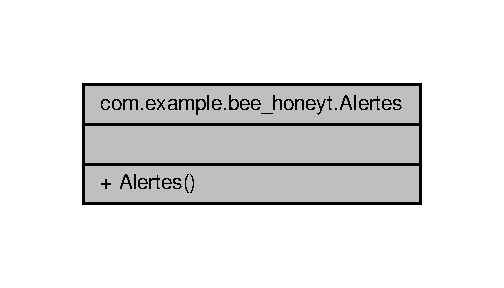
\includegraphics[width=242pt]{classcom_1_1example_1_1bee__honeyt_1_1_alertes__coll__graph}
\end{center}
\end{figure}
\subsubsection*{Fonctions membres publiques}
\begin{DoxyCompactItemize}
\item 
\hyperlink{classcom_1_1example_1_1bee__honeyt_1_1_alertes_a8a4cde771fa2eeea4df67f2b82b3958a}{Alertes} ()
\end{DoxyCompactItemize}


\subsubsection{Description détaillée}


Définition à la ligne \hyperlink{_alertes_8java_source_l00011}{11} du fichier \hyperlink{_alertes_8java_source}{Alertes.\+java}.



\subsubsection{Documentation des constructeurs et destructeur}
\mbox{\Hypertarget{classcom_1_1example_1_1bee__honeyt_1_1_alertes_a8a4cde771fa2eeea4df67f2b82b3958a}\label{classcom_1_1example_1_1bee__honeyt_1_1_alertes_a8a4cde771fa2eeea4df67f2b82b3958a}} 
\index{com\+::example\+::bee\+\_\+honeyt\+::\+Alertes@{com\+::example\+::bee\+\_\+honeyt\+::\+Alertes}!Alertes@{Alertes}}
\index{Alertes@{Alertes}!com\+::example\+::bee\+\_\+honeyt\+::\+Alertes@{com\+::example\+::bee\+\_\+honeyt\+::\+Alertes}}
\paragraph{\texorpdfstring{Alertes()}{Alertes()}}
{\footnotesize\ttfamily com.\+example.\+bee\+\_\+honeyt.\+Alertes.\+Alertes (\begin{DoxyParamCaption}{ }\end{DoxyParamCaption})}



Définition à la ligne \hyperlink{_alertes_8java_source_l00013}{13} du fichier \hyperlink{_alertes_8java_source}{Alertes.\+java}.


\begin{DoxyCode}
00014     \{
00015 
00016     \}
\end{DoxyCode}


La documentation de cette classe a été générée à partir du fichier suivant \+:\begin{DoxyCompactItemize}
\item 
\hyperlink{_alertes_8java}{Alertes.\+java}\end{DoxyCompactItemize}

\hypertarget{classcom_1_1example_1_1bee__honeyt_1_1_communication}{}\subsection{Référence de la classe com.\+example.\+bee\+\_\+honeyt.\+Communication}
\label{classcom_1_1example_1_1bee__honeyt_1_1_communication}\index{com.\+example.\+bee\+\_\+honeyt.\+Communication@{com.\+example.\+bee\+\_\+honeyt.\+Communication}}


Déclaration de la classe \hyperlink{classcom_1_1example_1_1bee__honeyt_1_1_communication}{Communication}.  




Graphe de collaboration de com.\+example.\+bee\+\_\+honeyt.\+Communication\+:\nopagebreak
\begin{figure}[H]
\begin{center}
\leavevmode
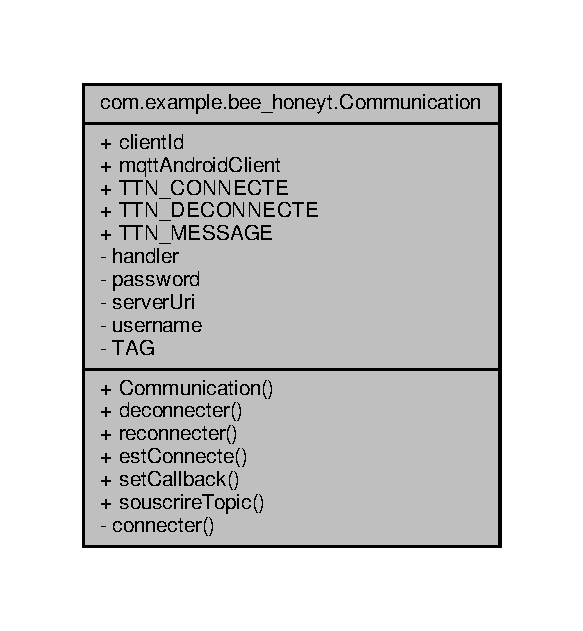
\includegraphics[width=280pt]{classcom_1_1example_1_1bee__honeyt_1_1_communication__coll__graph}
\end{center}
\end{figure}
\subsubsection*{Fonctions membres publiques}
\begin{DoxyCompactItemize}
\item 
\hyperlink{classcom_1_1example_1_1bee__honeyt_1_1_communication_a1f92cddc3a6b011683d0ed8d1371227d}{Communication} (Context context, final Handler \hyperlink{classcom_1_1example_1_1bee__honeyt_1_1_communication_add1a0705dba503c1c4c7a3168a571b20}{handler})
\begin{DoxyCompactList}\small\item\em Constructeur de la classe \hyperlink{classcom_1_1example_1_1bee__honeyt_1_1_communication}{Communication}. \end{DoxyCompactList}\item 
void \hyperlink{classcom_1_1example_1_1bee__honeyt_1_1_communication_a55454851f5e883b1539bd60fa7f4bfc6}{deconnecter} ()
\begin{DoxyCompactList}\small\item\em Deconnexion du T\+TN. \end{DoxyCompactList}\item 
void \hyperlink{classcom_1_1example_1_1bee__honeyt_1_1_communication_ae0851e23e515c71cfa06cf635c731c07}{reconnecter} ()
\begin{DoxyCompactList}\small\item\em Reconnexion au T\+TN. \end{DoxyCompactList}\end{DoxyCompactItemize}
\subsubsection*{Fonctions membres publiques statiques}
\begin{DoxyCompactItemize}
\item 
static boolean \hyperlink{classcom_1_1example_1_1bee__honeyt_1_1_communication_a155e0619c3d504750871a84e637bb808}{est\+Connecte} ()
\begin{DoxyCompactList}\small\item\em Retourne l\textquotesingle{}état de connexion au serveur T\+TN. \end{DoxyCompactList}\item 
static void \hyperlink{classcom_1_1example_1_1bee__honeyt_1_1_communication_a86faf903d7d230a0105b29e5c1d5f4a2}{set\+Callback} (Mqtt\+Callback\+Extended callback)
\begin{DoxyCompactList}\small\item\em Installe les fonctions de rappel. \end{DoxyCompactList}\item 
static boolean \hyperlink{classcom_1_1example_1_1bee__honeyt_1_1_communication_aa1093a3d4f3479595a36ef2425f3ef70}{souscrire\+Topic} (String device\+ID)
\begin{DoxyCompactList}\small\item\em S\textquotesingle{}abonne à un topic (device\+ID = E\+S\+P32 d\textquotesingle{}une ruche dans T\+TN) \end{DoxyCompactList}\end{DoxyCompactItemize}
\subsubsection*{Attributs publics statiques}
\begin{DoxyCompactItemize}
\item 
static String \hyperlink{classcom_1_1example_1_1bee__honeyt_1_1_communication_a8b44e0173d57396d5478f767723c23cc}{client\+Id} = \char`\"{}rucher\char`\"{}
\begin{DoxyCompactList}\small\item\em Application ID. \end{DoxyCompactList}\item 
static Mqtt\+Android\+Client \hyperlink{classcom_1_1example_1_1bee__honeyt_1_1_communication_a86db63a356e4638c1d39c54bbe64f0e1}{mqtt\+Android\+Client}
\item 
static final int \hyperlink{classcom_1_1example_1_1bee__honeyt_1_1_communication_ad8ad53a30dea0bfcc57bad80cb67ab92}{T\+T\+N\+\_\+\+C\+O\+N\+N\+E\+C\+TE} = 1
\item 
static final int \hyperlink{classcom_1_1example_1_1bee__honeyt_1_1_communication_ae2fba68d5f0ed6c8bdbaaae68a4e6192}{T\+T\+N\+\_\+\+D\+E\+C\+O\+N\+N\+E\+C\+TE} = 2
\item 
static final int \hyperlink{classcom_1_1example_1_1bee__honeyt_1_1_communication_aa81848662846946c92ee2b1380669c66}{T\+T\+N\+\_\+\+M\+E\+S\+S\+A\+GE} = 3
\end{DoxyCompactItemize}
\subsubsection*{Fonctions membres privées}
\begin{DoxyCompactItemize}
\item 
void \hyperlink{classcom_1_1example_1_1bee__honeyt_1_1_communication_aadc176b28bce357bf655d0feec024013}{connecter} ()
\begin{DoxyCompactList}\small\item\em Connexion au T\+TN. \end{DoxyCompactList}\end{DoxyCompactItemize}
\subsubsection*{Attributs privés}
\begin{DoxyCompactItemize}
\item 
Handler \hyperlink{classcom_1_1example_1_1bee__honeyt_1_1_communication_add1a0705dba503c1c4c7a3168a571b20}{handler} = null
\item 
String \hyperlink{classcom_1_1example_1_1bee__honeyt_1_1_communication_ace9fdd48d010e4c43cb5d32767207cae}{password} = \char`\"{}ttn-\/account-\/v2.\+a4\+G\+Rsjlo\+Pz\+Q\+\_\+4hswG-\/rm\+Wa\+O9\+Mz\+Wk\+Atz\+Cvgg\+We\+O2\+Dv\+L4\char`\"{}
\begin{DoxyCompactList}\small\item\em mot de passe T\+TN \end{DoxyCompactList}\item 
String \hyperlink{classcom_1_1example_1_1bee__honeyt_1_1_communication_a19b957478f8d8a0d8319e8459d85862e}{server\+Uri} = \char`\"{}tcp\+://eu.\+thethings.\+network\+:1883\char`\"{}
\begin{DoxyCompactList}\small\item\em lien vers T\+TN \end{DoxyCompactList}\item 
String \hyperlink{classcom_1_1example_1_1bee__honeyt_1_1_communication_abfc9c112404b1ddf0fa90587201d5a8f}{username} = \char`\"{}rucher\char`\"{}
\begin{DoxyCompactList}\small\item\em nom d\textquotesingle{}utilisateur \end{DoxyCompactList}\end{DoxyCompactItemize}
\subsubsection*{Attributs privés statiques}
\begin{DoxyCompactItemize}
\item 
static final String \hyperlink{classcom_1_1example_1_1bee__honeyt_1_1_communication_a848338dd9654af654c7e681742666785}{T\+AG} = \char`\"{}\+\_\+\+Communication\char`\"{}
\end{DoxyCompactItemize}


\subsubsection{Description détaillée}
Déclaration de la classe \hyperlink{classcom_1_1example_1_1bee__honeyt_1_1_communication}{Communication}. 

Permet la communication M\+Q\+TT avec le serveur The Things Network \begin{DoxyAuthor}{Auteur}
Thierry Vaira 
\end{DoxyAuthor}
\begin{DoxyParagraph}{Last\+Changed\+Revision}
76 
\end{DoxyParagraph}
\begin{DoxyParagraph}{Last\+Changed\+Date}
2021-\/04-\/28 12\+:22\+:56 +0200 (mer. 28 avril 2021) 
\end{DoxyParagraph}


Définition à la ligne \hyperlink{_communication_8java_source_l00028}{28} du fichier \hyperlink{_communication_8java_source}{Communication.\+java}.



\subsubsection{Documentation des constructeurs et destructeur}
\mbox{\Hypertarget{classcom_1_1example_1_1bee__honeyt_1_1_communication_a1f92cddc3a6b011683d0ed8d1371227d}\label{classcom_1_1example_1_1bee__honeyt_1_1_communication_a1f92cddc3a6b011683d0ed8d1371227d}} 
\index{com\+::example\+::bee\+\_\+honeyt\+::\+Communication@{com\+::example\+::bee\+\_\+honeyt\+::\+Communication}!Communication@{Communication}}
\index{Communication@{Communication}!com\+::example\+::bee\+\_\+honeyt\+::\+Communication@{com\+::example\+::bee\+\_\+honeyt\+::\+Communication}}
\paragraph{\texorpdfstring{Communication()}{Communication()}}
{\footnotesize\ttfamily com.\+example.\+bee\+\_\+honeyt.\+Communication.\+Communication (\begin{DoxyParamCaption}\item[{Context}]{context,  }\item[{final Handler}]{handler }\end{DoxyParamCaption})}



Constructeur de la classe \hyperlink{classcom_1_1example_1_1bee__honeyt_1_1_communication}{Communication}. 


\begin{DoxyParams}{Paramètres}
{\em context} & \\
\hline
{\em handler} & \\
\hline
\end{DoxyParams}


Définition à la ligne \hyperlink{_communication_8java_source_l00063}{63} du fichier \hyperlink{_communication_8java_source}{Communication.\+java}.



Références \hyperlink{_communication_8java_source_l00131}{com.\+example.\+bee\+\_\+honeyt.\+Communication.\+connecter()}, et \hyperlink{_communication_8java_source_l00039}{com.\+example.\+bee\+\_\+honeyt.\+Communication.\+handler}.


\begin{DoxyCode}
00064     \{
00065         Log.v(\hyperlink{classcom_1_1example_1_1bee__honeyt_1_1_communication_a848338dd9654af654c7e681742666785}{TAG}, \textcolor{stringliteral}{"[Communication()] clientId = "} + \hyperlink{classcom_1_1example_1_1bee__honeyt_1_1_communication_a8b44e0173d57396d5478f767723c23cc}{clientId});
00066         this.\hyperlink{classcom_1_1example_1_1bee__honeyt_1_1_communication_add1a0705dba503c1c4c7a3168a571b20}{handler} = \hyperlink{classcom_1_1example_1_1bee__honeyt_1_1_communication_add1a0705dba503c1c4c7a3168a571b20}{handler};
00067         \hyperlink{classcom_1_1example_1_1bee__honeyt_1_1_communication_a86db63a356e4638c1d39c54bbe64f0e1}{mqttAndroidClient} = \textcolor{keyword}{new} MqttAndroidClient(context, 
      \hyperlink{classcom_1_1example_1_1bee__honeyt_1_1_communication_a19b957478f8d8a0d8319e8459d85862e}{serverUri}, \hyperlink{classcom_1_1example_1_1bee__honeyt_1_1_communication_a8b44e0173d57396d5478f767723c23cc}{clientId});
00068         \hyperlink{classcom_1_1example_1_1bee__honeyt_1_1_communication_a86db63a356e4638c1d39c54bbe64f0e1}{mqttAndroidClient}.setCallback(\textcolor{keyword}{new} MqttCallbackExtended()
00069         \{
00070             @Override
00071             \textcolor{keyword}{public} \textcolor{keywordtype}{void} connectComplete(\textcolor{keywordtype}{boolean} b, String s)
00072             \{
00073                 Log.w(\hyperlink{classcom_1_1example_1_1bee__honeyt_1_1_communication_a848338dd9654af654c7e681742666785}{TAG}, \textcolor{stringliteral}{"[connectComplete()] serverUri = "} + s + \textcolor{stringliteral}{" connecte = "} + 
      \hyperlink{classcom_1_1example_1_1bee__honeyt_1_1_communication_a86db63a356e4638c1d39c54bbe64f0e1}{mqttAndroidClient}.isConnected());
00074                 Message msg = Message.obtain();
00075                 Bundle bundle = \textcolor{keyword}{new} Bundle();
00076                 bundle.putInt(\textcolor{stringliteral}{"etat"}, \hyperlink{classcom_1_1example_1_1bee__honeyt_1_1_communication_ad8ad53a30dea0bfcc57bad80cb67ab92}{TTN\_CONNECTE}); \textcolor{comment}{// clé -> valeur ici etat -> TTN\_CONNECTE}
00077                 msg.setData(bundle);
00078                 \hyperlink{classcom_1_1example_1_1bee__honeyt_1_1_communication_add1a0705dba503c1c4c7a3168a571b20}{handler}.sendMessage(msg);
00079             \}
00080 
00081             @Override
00082             \textcolor{keyword}{public} \textcolor{keywordtype}{void} connectionLost(Throwable throwable)
00083             \{
00084                 Log.w(\hyperlink{classcom_1_1example_1_1bee__honeyt_1_1_communication_a848338dd9654af654c7e681742666785}{TAG}, \textcolor{stringliteral}{"[connectionLost()]"});
00085                 Message msg = Message.obtain();
00086                 Bundle b = \textcolor{keyword}{new} Bundle();
00087                 b.putInt(\textcolor{stringliteral}{"etat"}, \hyperlink{classcom_1_1example_1_1bee__honeyt_1_1_communication_ae2fba68d5f0ed6c8bdbaaae68a4e6192}{TTN\_DECONNECTE});
00088                 msg.setData(b);
00089                 \hyperlink{classcom_1_1example_1_1bee__honeyt_1_1_communication_add1a0705dba503c1c4c7a3168a571b20}{handler}.sendMessage(msg);
00090             \}
00091 
00092             @Override
00093             \textcolor{keyword}{public} \textcolor{keywordtype}{void} messageArrived(String topic, MqttMessage mqttMessage) \textcolor{keywordflow}{throws} Exception
00094             \{
00095                 Log.w(\hyperlink{classcom_1_1example_1_1bee__honeyt_1_1_communication_a848338dd9654af654c7e681742666785}{TAG}, \textcolor{stringliteral}{"[messageArrived()] topic = "} + topic + \textcolor{stringliteral}{" message = "} + mqttMessage.toString(
      ));
00096                 Message msg = Message.obtain();
00097                 Bundle b = \textcolor{keyword}{new} Bundle();
00098                 b.putInt(\textcolor{stringliteral}{"etat"}, \hyperlink{classcom_1_1example_1_1bee__honeyt_1_1_communication_aa81848662846946c92ee2b1380669c66}{TTN\_MESSAGE});
00099                 b.putString(\textcolor{stringliteral}{"topic"}, topic);
00100                 b.putString(\textcolor{stringliteral}{"message"}, mqttMessage.toString());
00101                 msg.setData(b);
00102                 \hyperlink{classcom_1_1example_1_1bee__honeyt_1_1_communication_add1a0705dba503c1c4c7a3168a571b20}{handler}.sendMessage(msg);
00103             \}
00104 
00105             @Override
00106             \textcolor{keyword}{public} \textcolor{keywordtype}{void} deliveryComplete(IMqttDeliveryToken iMqttDeliveryToken)
00107             \{
00108                 Log.w(\hyperlink{classcom_1_1example_1_1bee__honeyt_1_1_communication_a848338dd9654af654c7e681742666785}{TAG}, \textcolor{stringliteral}{"[deliveryComplete()]"});
00109             \}
00110         \});
00111 
00112         \hyperlink{classcom_1_1example_1_1bee__honeyt_1_1_communication_aadc176b28bce357bf655d0feec024013}{connecter}();
00113     \}
\end{DoxyCode}


\subsubsection{Documentation des fonctions membres}
\mbox{\Hypertarget{classcom_1_1example_1_1bee__honeyt_1_1_communication_aadc176b28bce357bf655d0feec024013}\label{classcom_1_1example_1_1bee__honeyt_1_1_communication_aadc176b28bce357bf655d0feec024013}} 
\index{com\+::example\+::bee\+\_\+honeyt\+::\+Communication@{com\+::example\+::bee\+\_\+honeyt\+::\+Communication}!connecter@{connecter}}
\index{connecter@{connecter}!com\+::example\+::bee\+\_\+honeyt\+::\+Communication@{com\+::example\+::bee\+\_\+honeyt\+::\+Communication}}
\paragraph{\texorpdfstring{connecter()}{connecter()}}
{\footnotesize\ttfamily com.\+example.\+bee\+\_\+honeyt.\+Communication.\+connecter (\begin{DoxyParamCaption}{ }\end{DoxyParamCaption})\hspace{0.3cm}{\ttfamily [private]}}



Connexion au T\+TN. 



Définition à la ligne \hyperlink{_communication_8java_source_l00131}{131} du fichier \hyperlink{_communication_8java_source}{Communication.\+java}.



Référencé par \hyperlink{_communication_8java_source_l00063}{com.\+example.\+bee\+\_\+honeyt.\+Communication.\+Communication()}, et \hyperlink{_communication_8java_source_l00174}{com.\+example.\+bee\+\_\+honeyt.\+Communication.\+reconnecter()}.


\begin{DoxyCode}
00132     \{
00133         MqttConnectOptions mqttConnectOptions = \textcolor{keyword}{new} MqttConnectOptions();
00134         mqttConnectOptions.setAutomaticReconnect(\textcolor{keyword}{true});
00135         mqttConnectOptions.setCleanSession(\textcolor{keyword}{false});
00136         mqttConnectOptions.setUserName(\hyperlink{classcom_1_1example_1_1bee__honeyt_1_1_communication_abfc9c112404b1ddf0fa90587201d5a8f}{username});
00137         mqttConnectOptions.setPassword(\hyperlink{classcom_1_1example_1_1bee__honeyt_1_1_communication_ace9fdd48d010e4c43cb5d32767207cae}{password}.toCharArray());
00138 
00139         \textcolor{keywordflow}{try}
00140         \{
00141             Log.d(\hyperlink{classcom_1_1example_1_1bee__honeyt_1_1_communication_a848338dd9654af654c7e681742666785}{TAG}, \textcolor{stringliteral}{"[connecter()] serverUri = "} + \hyperlink{classcom_1_1example_1_1bee__honeyt_1_1_communication_a19b957478f8d8a0d8319e8459d85862e}{serverUri} + \textcolor{stringliteral}{" clientId = "} + 
      \hyperlink{classcom_1_1example_1_1bee__honeyt_1_1_communication_a8b44e0173d57396d5478f767723c23cc}{clientId});
00142             \hyperlink{classcom_1_1example_1_1bee__honeyt_1_1_communication_a86db63a356e4638c1d39c54bbe64f0e1}{mqttAndroidClient}.connect(mqttConnectOptions, null, \textcolor{keyword}{new} IMqttActionListener()
00143             \{
00144                 @Override
00145                 \textcolor{keyword}{public} \textcolor{keywordtype}{void} onSuccess(IMqttToken asyncActionToken)
00146                 \{
00147                     DisconnectedBufferOptions disconnectedBufferOptions = \textcolor{keyword}{new} DisconnectedBufferOptions();
00148                     disconnectedBufferOptions.setBufferEnabled(\textcolor{keyword}{true});
00149                     disconnectedBufferOptions.setBufferSize(100);
00150                     disconnectedBufferOptions.setPersistBuffer(\textcolor{keyword}{false});
00151                     disconnectedBufferOptions.setDeleteOldestMessages(\textcolor{keyword}{false});
00152                     \hyperlink{classcom_1_1example_1_1bee__honeyt_1_1_communication_a86db63a356e4638c1d39c54bbe64f0e1}{mqttAndroidClient}.setBufferOpts(disconnectedBufferOptions);
00153                     Log.d(\hyperlink{classcom_1_1example_1_1bee__honeyt_1_1_communication_a848338dd9654af654c7e681742666785}{TAG}, \textcolor{stringliteral}{"[onSuccess()] serverUri = "} + \hyperlink{classcom_1_1example_1_1bee__honeyt_1_1_communication_a19b957478f8d8a0d8319e8459d85862e}{serverUri} + \textcolor{stringliteral}{" clientId = "} + 
      \hyperlink{classcom_1_1example_1_1bee__honeyt_1_1_communication_a8b44e0173d57396d5478f767723c23cc}{clientId});
00154                 \}
00155 
00156                 @Override
00157                 \textcolor{keyword}{public} \textcolor{keywordtype}{void} onFailure(IMqttToken asyncActionToken, Throwable exception)
00158                 \{
00159                     Log.d(\hyperlink{classcom_1_1example_1_1bee__honeyt_1_1_communication_a848338dd9654af654c7e681742666785}{TAG}, \textcolor{stringliteral}{"[onFailure()] serverUri = "} + \hyperlink{classcom_1_1example_1_1bee__honeyt_1_1_communication_a19b957478f8d8a0d8319e8459d85862e}{serverUri} + \textcolor{stringliteral}{" clientId = "} + 
      \hyperlink{classcom_1_1example_1_1bee__honeyt_1_1_communication_a8b44e0173d57396d5478f767723c23cc}{clientId} + \textcolor{stringliteral}{" exception = "} + exception.toString());
00160                 \}
00161             \});
00162         \}
00163         \textcolor{keywordflow}{catch} (MqttException e)
00164         \{
00165             e.printStackTrace();
00166         \}
00167     \}
\end{DoxyCode}
\mbox{\Hypertarget{classcom_1_1example_1_1bee__honeyt_1_1_communication_a55454851f5e883b1539bd60fa7f4bfc6}\label{classcom_1_1example_1_1bee__honeyt_1_1_communication_a55454851f5e883b1539bd60fa7f4bfc6}} 
\index{com\+::example\+::bee\+\_\+honeyt\+::\+Communication@{com\+::example\+::bee\+\_\+honeyt\+::\+Communication}!deconnecter@{deconnecter}}
\index{deconnecter@{deconnecter}!com\+::example\+::bee\+\_\+honeyt\+::\+Communication@{com\+::example\+::bee\+\_\+honeyt\+::\+Communication}}
\paragraph{\texorpdfstring{deconnecter()}{deconnecter()}}
{\footnotesize\ttfamily com.\+example.\+bee\+\_\+honeyt.\+Communication.\+deconnecter (\begin{DoxyParamCaption}{ }\end{DoxyParamCaption})}



Deconnexion du T\+TN. 



Définition à la ligne \hyperlink{_communication_8java_source_l00187}{187} du fichier \hyperlink{_communication_8java_source}{Communication.\+java}.



Référencé par \hyperlink{_communication_8java_source_l00174}{com.\+example.\+bee\+\_\+honeyt.\+Communication.\+reconnecter()}.


\begin{DoxyCode}
00188     \{
00189         Log.d(\hyperlink{classcom_1_1example_1_1bee__honeyt_1_1_communication_a848338dd9654af654c7e681742666785}{TAG}, \textcolor{stringliteral}{"[deconnecter()] serverUri = "} + \hyperlink{classcom_1_1example_1_1bee__honeyt_1_1_communication_a19b957478f8d8a0d8319e8459d85862e}{serverUri} + \textcolor{stringliteral}{" clientId = "} + 
      \hyperlink{classcom_1_1example_1_1bee__honeyt_1_1_communication_a8b44e0173d57396d5478f767723c23cc}{clientId});
00190         \textcolor{keywordflow}{try}
00191         \{
00192             IMqttToken disconToken = \hyperlink{classcom_1_1example_1_1bee__honeyt_1_1_communication_a86db63a356e4638c1d39c54bbe64f0e1}{mqttAndroidClient}.disconnect();
00193             disconToken.setActionCallback(\textcolor{keyword}{new} IMqttActionListener()
00194             \{
00195                 @Override
00196                 \textcolor{keyword}{public} \textcolor{keywordtype}{void} onSuccess(IMqttToken asyncActionToken)
00197                 \{
00198                     Log.d(\hyperlink{classcom_1_1example_1_1bee__honeyt_1_1_communication_a848338dd9654af654c7e681742666785}{TAG}, \textcolor{stringliteral}{"[onSuccess()] serverUri = "} + \hyperlink{classcom_1_1example_1_1bee__honeyt_1_1_communication_a19b957478f8d8a0d8319e8459d85862e}{serverUri} + \textcolor{stringliteral}{" clientId = "} + 
      \hyperlink{classcom_1_1example_1_1bee__honeyt_1_1_communication_a8b44e0173d57396d5478f767723c23cc}{clientId});
00199                 \}
00200 
00201                 @Override
00202                 \textcolor{keyword}{public} \textcolor{keywordtype}{void} onFailure(IMqttToken asyncActionToken, Throwable exception)
00203                 \{
00204                     Log.d(\hyperlink{classcom_1_1example_1_1bee__honeyt_1_1_communication_a848338dd9654af654c7e681742666785}{TAG}, \textcolor{stringliteral}{"[onFailure()] serverUri = "} + \hyperlink{classcom_1_1example_1_1bee__honeyt_1_1_communication_a19b957478f8d8a0d8319e8459d85862e}{serverUri} + \textcolor{stringliteral}{" clientId = "} + 
      \hyperlink{classcom_1_1example_1_1bee__honeyt_1_1_communication_a8b44e0173d57396d5478f767723c23cc}{clientId} + \textcolor{stringliteral}{" exception = "} + exception.toString());
00205                 \}
00206             \});
00207         \}
00208         \textcolor{keywordflow}{catch} (MqttException e)
00209         \{
00210             e.printStackTrace();
00211         \}
00212     \}
\end{DoxyCode}
\mbox{\Hypertarget{classcom_1_1example_1_1bee__honeyt_1_1_communication_a155e0619c3d504750871a84e637bb808}\label{classcom_1_1example_1_1bee__honeyt_1_1_communication_a155e0619c3d504750871a84e637bb808}} 
\index{com\+::example\+::bee\+\_\+honeyt\+::\+Communication@{com\+::example\+::bee\+\_\+honeyt\+::\+Communication}!est\+Connecte@{est\+Connecte}}
\index{est\+Connecte@{est\+Connecte}!com\+::example\+::bee\+\_\+honeyt\+::\+Communication@{com\+::example\+::bee\+\_\+honeyt\+::\+Communication}}
\paragraph{\texorpdfstring{est\+Connecte()}{estConnecte()}}
{\footnotesize\ttfamily com.\+example.\+bee\+\_\+honeyt.\+Communication.\+est\+Connecte (\begin{DoxyParamCaption}{ }\end{DoxyParamCaption})\hspace{0.3cm}{\ttfamily [static]}}



Retourne l\textquotesingle{}état de connexion au serveur T\+TN. 



Définition à la ligne \hyperlink{_communication_8java_source_l00219}{219} du fichier \hyperlink{_communication_8java_source}{Communication.\+java}.



Référencé par \hyperlink{_communication_8java_source_l00174}{com.\+example.\+bee\+\_\+honeyt.\+Communication.\+reconnecter()}.


\begin{DoxyCode}
00220     \{
00221         Log.w(\hyperlink{classcom_1_1example_1_1bee__honeyt_1_1_communication_a848338dd9654af654c7e681742666785}{TAG}, \textcolor{stringliteral}{"[estConnecte()] "} + \hyperlink{classcom_1_1example_1_1bee__honeyt_1_1_communication_a86db63a356e4638c1d39c54bbe64f0e1}{mqttAndroidClient}.isConnected());
00222 
00223         \textcolor{keywordflow}{return} \hyperlink{classcom_1_1example_1_1bee__honeyt_1_1_communication_a86db63a356e4638c1d39c54bbe64f0e1}{mqttAndroidClient}.isConnected();
00224     \}
\end{DoxyCode}
\mbox{\Hypertarget{classcom_1_1example_1_1bee__honeyt_1_1_communication_ae0851e23e515c71cfa06cf635c731c07}\label{classcom_1_1example_1_1bee__honeyt_1_1_communication_ae0851e23e515c71cfa06cf635c731c07}} 
\index{com\+::example\+::bee\+\_\+honeyt\+::\+Communication@{com\+::example\+::bee\+\_\+honeyt\+::\+Communication}!reconnecter@{reconnecter}}
\index{reconnecter@{reconnecter}!com\+::example\+::bee\+\_\+honeyt\+::\+Communication@{com\+::example\+::bee\+\_\+honeyt\+::\+Communication}}
\paragraph{\texorpdfstring{reconnecter()}{reconnecter()}}
{\footnotesize\ttfamily com.\+example.\+bee\+\_\+honeyt.\+Communication.\+reconnecter (\begin{DoxyParamCaption}{ }\end{DoxyParamCaption})}



Reconnexion au T\+TN. 



Définition à la ligne \hyperlink{_communication_8java_source_l00174}{174} du fichier \hyperlink{_communication_8java_source}{Communication.\+java}.



Références \hyperlink{_communication_8java_source_l00131}{com.\+example.\+bee\+\_\+honeyt.\+Communication.\+connecter()}, \hyperlink{_communication_8java_source_l00187}{com.\+example.\+bee\+\_\+honeyt.\+Communication.\+deconnecter()}, et \hyperlink{_communication_8java_source_l00219}{com.\+example.\+bee\+\_\+honeyt.\+Communication.\+est\+Connecte()}.


\begin{DoxyCode}
00175     \{
00176         Log.w(\hyperlink{classcom_1_1example_1_1bee__honeyt_1_1_communication_a848338dd9654af654c7e681742666785}{TAG}, \textcolor{stringliteral}{"[reconnecter()]"});
00177         \textcolor{keywordflow}{if} (\hyperlink{classcom_1_1example_1_1bee__honeyt_1_1_communication_a155e0619c3d504750871a84e637bb808}{estConnecte}())
00178             \hyperlink{classcom_1_1example_1_1bee__honeyt_1_1_communication_a55454851f5e883b1539bd60fa7f4bfc6}{deconnecter}();
00179         \hyperlink{classcom_1_1example_1_1bee__honeyt_1_1_communication_aadc176b28bce357bf655d0feec024013}{connecter}();
00180     \}
\end{DoxyCode}
\mbox{\Hypertarget{classcom_1_1example_1_1bee__honeyt_1_1_communication_a86faf903d7d230a0105b29e5c1d5f4a2}\label{classcom_1_1example_1_1bee__honeyt_1_1_communication_a86faf903d7d230a0105b29e5c1d5f4a2}} 
\index{com\+::example\+::bee\+\_\+honeyt\+::\+Communication@{com\+::example\+::bee\+\_\+honeyt\+::\+Communication}!set\+Callback@{set\+Callback}}
\index{set\+Callback@{set\+Callback}!com\+::example\+::bee\+\_\+honeyt\+::\+Communication@{com\+::example\+::bee\+\_\+honeyt\+::\+Communication}}
\paragraph{\texorpdfstring{set\+Callback()}{setCallback()}}
{\footnotesize\ttfamily com.\+example.\+bee\+\_\+honeyt.\+Communication.\+set\+Callback (\begin{DoxyParamCaption}\item[{Mqtt\+Callback\+Extended}]{callback }\end{DoxyParamCaption})\hspace{0.3cm}{\ttfamily [static]}}



Installe les fonctions de rappel. 


\begin{DoxyParams}{Paramètres}
{\em callback} & le retour \\
\hline
\end{DoxyParams}


Définition à la ligne \hyperlink{_communication_8java_source_l00121}{121} du fichier \hyperlink{_communication_8java_source}{Communication.\+java}.


\begin{DoxyCode}
00122     \{
00123         \hyperlink{classcom_1_1example_1_1bee__honeyt_1_1_communication_a86db63a356e4638c1d39c54bbe64f0e1}{mqttAndroidClient}.setCallback(callback);
00124     \}
\end{DoxyCode}
\mbox{\Hypertarget{classcom_1_1example_1_1bee__honeyt_1_1_communication_aa1093a3d4f3479595a36ef2425f3ef70}\label{classcom_1_1example_1_1bee__honeyt_1_1_communication_aa1093a3d4f3479595a36ef2425f3ef70}} 
\index{com\+::example\+::bee\+\_\+honeyt\+::\+Communication@{com\+::example\+::bee\+\_\+honeyt\+::\+Communication}!souscrire\+Topic@{souscrire\+Topic}}
\index{souscrire\+Topic@{souscrire\+Topic}!com\+::example\+::bee\+\_\+honeyt\+::\+Communication@{com\+::example\+::bee\+\_\+honeyt\+::\+Communication}}
\paragraph{\texorpdfstring{souscrire\+Topic()}{souscrireTopic()}}
{\footnotesize\ttfamily com.\+example.\+bee\+\_\+honeyt.\+Communication.\+souscrire\+Topic (\begin{DoxyParamCaption}\item[{String}]{topic }\end{DoxyParamCaption})\hspace{0.3cm}{\ttfamily [static]}}



S\textquotesingle{}abonne à un topic (device\+ID = E\+S\+P32 d\textquotesingle{}une ruche dans T\+TN) 


\begin{DoxyParams}{Paramètres}
{\em device\+ID} & le device\+ID dans T\+TN \\
\hline
\end{DoxyParams}


Définition à la ligne \hyperlink{_communication_8java_source_l00232}{232} du fichier \hyperlink{_communication_8java_source}{Communication.\+java}.



Référencé par \hyperlink{_i_h_m_mobile_8java_source_l00563}{com.\+example.\+bee\+\_\+honeyt.\+I\+H\+M\+Mobile.\+abonner\+Ruches()}.


\begin{DoxyCode}
00233     \{
00234         \textcolor{comment}{// Vérifications}
00235         \textcolor{keywordflow}{if}(\hyperlink{classcom_1_1example_1_1bee__honeyt_1_1_communication_a86db63a356e4638c1d39c54bbe64f0e1}{mqttAndroidClient} == null && !\hyperlink{classcom_1_1example_1_1bee__honeyt_1_1_communication_a86db63a356e4638c1d39c54bbe64f0e1}{mqttAndroidClient}.isConnected())
00236         \{
00237             \textcolor{keywordflow}{return} \textcolor{keyword}{false};
00238         \}
00239 
00240         \textcolor{keyword}{final} String topicTTN = \hyperlink{classcom_1_1example_1_1bee__honeyt_1_1_communication_a8b44e0173d57396d5478f767723c23cc}{clientId} + \textcolor{stringliteral}{"/devices/"} + deviceID + \textcolor{stringliteral}{"/up"};
00241         Log.w(\hyperlink{classcom_1_1example_1_1bee__honeyt_1_1_communication_a848338dd9654af654c7e681742666785}{TAG}, \textcolor{stringliteral}{"[souscrireTopic()] topic = "} + topicTTN);
00242         \textcolor{keywordflow}{try}
00243         \{
00244             \textcolor{keyword}{final} \textcolor{keywordtype}{boolean}[] retour = \{\textcolor{keyword}{false}\};
00245             \hyperlink{classcom_1_1example_1_1bee__honeyt_1_1_communication_a86db63a356e4638c1d39c54bbe64f0e1}{mqttAndroidClient}.subscribe(topicTTN, 0, null, \textcolor{keyword}{new} IMqttActionListener()
00246             \{
00247                 @Override
00248                 \textcolor{keyword}{public} \textcolor{keywordtype}{void} onSuccess(IMqttToken asyncActionToken)
00249                 \{
00250                     Log.w(\hyperlink{classcom_1_1example_1_1bee__honeyt_1_1_communication_a848338dd9654af654c7e681742666785}{TAG}, \textcolor{stringliteral}{"[onSuccess()] topic = "} + topicTTN);
00251                     retour[0] = \textcolor{keyword}{true};
00252                 \}
00253 
00254                 @Override
00255                 \textcolor{keyword}{public} \textcolor{keywordtype}{void} onFailure(IMqttToken asyncActionToken, Throwable exception)
00256                 \{
00257                     Log.w(\hyperlink{classcom_1_1example_1_1bee__honeyt_1_1_communication_a848338dd9654af654c7e681742666785}{TAG}, \textcolor{stringliteral}{"[onFailure()] topic = "} + topicTTN);
00258                     retour[0] = \textcolor{keyword}{false};
00259                 \}
00260             \});
00261             \textcolor{keywordflow}{return} retour[0];
00262         \}
00263         \textcolor{keywordflow}{catch} (MqttException e)
00264         \{
00265             Log.w(\hyperlink{classcom_1_1example_1_1bee__honeyt_1_1_communication_a848338dd9654af654c7e681742666785}{TAG}, \textcolor{stringliteral}{"Erreur topic = "} + topicTTN);
00266             e.printStackTrace();
00267             \textcolor{keywordflow}{return} \textcolor{keyword}{false};
00268         \}
00269     \}
\end{DoxyCode}


\subsubsection{Documentation des données membres}
\mbox{\Hypertarget{classcom_1_1example_1_1bee__honeyt_1_1_communication_a8b44e0173d57396d5478f767723c23cc}\label{classcom_1_1example_1_1bee__honeyt_1_1_communication_a8b44e0173d57396d5478f767723c23cc}} 
\index{com\+::example\+::bee\+\_\+honeyt\+::\+Communication@{com\+::example\+::bee\+\_\+honeyt\+::\+Communication}!client\+Id@{client\+Id}}
\index{client\+Id@{client\+Id}!com\+::example\+::bee\+\_\+honeyt\+::\+Communication@{com\+::example\+::bee\+\_\+honeyt\+::\+Communication}}
\paragraph{\texorpdfstring{client\+Id}{clientId}}
{\footnotesize\ttfamily String com.\+example.\+bee\+\_\+honeyt.\+Communication.\+client\+Id = \char`\"{}rucher\char`\"{}\hspace{0.3cm}{\ttfamily [static]}}



Application ID. 

\begin{DoxyRefDesc}{A faire}
\item[\hyperlink{todo__todo000001}{A faire}]Prévoir une solution pour configurer/stocker les paramètres de connexion T\+TN \end{DoxyRefDesc}


Définition à la ligne \hyperlink{_communication_8java_source_l00052}{52} du fichier \hyperlink{_communication_8java_source}{Communication.\+java}.

\mbox{\Hypertarget{classcom_1_1example_1_1bee__honeyt_1_1_communication_add1a0705dba503c1c4c7a3168a571b20}\label{classcom_1_1example_1_1bee__honeyt_1_1_communication_add1a0705dba503c1c4c7a3168a571b20}} 
\index{com\+::example\+::bee\+\_\+honeyt\+::\+Communication@{com\+::example\+::bee\+\_\+honeyt\+::\+Communication}!handler@{handler}}
\index{handler@{handler}!com\+::example\+::bee\+\_\+honeyt\+::\+Communication@{com\+::example\+::bee\+\_\+honeyt\+::\+Communication}}
\paragraph{\texorpdfstring{handler}{handler}}
{\footnotesize\ttfamily Handler com.\+example.\+bee\+\_\+honeyt.\+Communication.\+handler = null\hspace{0.3cm}{\ttfamily [private]}}



Définition à la ligne \hyperlink{_communication_8java_source_l00039}{39} du fichier \hyperlink{_communication_8java_source}{Communication.\+java}.



Référencé par \hyperlink{_communication_8java_source_l00063}{com.\+example.\+bee\+\_\+honeyt.\+Communication.\+Communication()}.

\mbox{\Hypertarget{classcom_1_1example_1_1bee__honeyt_1_1_communication_a86db63a356e4638c1d39c54bbe64f0e1}\label{classcom_1_1example_1_1bee__honeyt_1_1_communication_a86db63a356e4638c1d39c54bbe64f0e1}} 
\index{com\+::example\+::bee\+\_\+honeyt\+::\+Communication@{com\+::example\+::bee\+\_\+honeyt\+::\+Communication}!mqtt\+Android\+Client@{mqtt\+Android\+Client}}
\index{mqtt\+Android\+Client@{mqtt\+Android\+Client}!com\+::example\+::bee\+\_\+honeyt\+::\+Communication@{com\+::example\+::bee\+\_\+honeyt\+::\+Communication}}
\paragraph{\texorpdfstring{mqtt\+Android\+Client}{mqttAndroidClient}}
{\footnotesize\ttfamily Mqtt\+Android\+Client com.\+example.\+bee\+\_\+honeyt.\+Communication.\+mqtt\+Android\+Client\hspace{0.3cm}{\ttfamily [static]}}

Attributs 

Définition à la ligne \hyperlink{_communication_8java_source_l00038}{38} du fichier \hyperlink{_communication_8java_source}{Communication.\+java}.

\mbox{\Hypertarget{classcom_1_1example_1_1bee__honeyt_1_1_communication_ace9fdd48d010e4c43cb5d32767207cae}\label{classcom_1_1example_1_1bee__honeyt_1_1_communication_ace9fdd48d010e4c43cb5d32767207cae}} 
\index{com\+::example\+::bee\+\_\+honeyt\+::\+Communication@{com\+::example\+::bee\+\_\+honeyt\+::\+Communication}!password@{password}}
\index{password@{password}!com\+::example\+::bee\+\_\+honeyt\+::\+Communication@{com\+::example\+::bee\+\_\+honeyt\+::\+Communication}}
\paragraph{\texorpdfstring{password}{password}}
{\footnotesize\ttfamily String com.\+example.\+bee\+\_\+honeyt.\+Communication.\+password = \char`\"{}ttn-\/account-\/v2.\+a4\+G\+Rsjlo\+Pz\+Q\+\_\+4hswG-\/rm\+Wa\+O9\+Mz\+Wk\+Atz\+Cvgg\+We\+O2\+Dv\+L4\char`\"{}\hspace{0.3cm}{\ttfamily [private]}}



mot de passe T\+TN 



Définition à la ligne \hyperlink{_communication_8java_source_l00054}{54} du fichier \hyperlink{_communication_8java_source}{Communication.\+java}.

\mbox{\Hypertarget{classcom_1_1example_1_1bee__honeyt_1_1_communication_a19b957478f8d8a0d8319e8459d85862e}\label{classcom_1_1example_1_1bee__honeyt_1_1_communication_a19b957478f8d8a0d8319e8459d85862e}} 
\index{com\+::example\+::bee\+\_\+honeyt\+::\+Communication@{com\+::example\+::bee\+\_\+honeyt\+::\+Communication}!server\+Uri@{server\+Uri}}
\index{server\+Uri@{server\+Uri}!com\+::example\+::bee\+\_\+honeyt\+::\+Communication@{com\+::example\+::bee\+\_\+honeyt\+::\+Communication}}
\paragraph{\texorpdfstring{server\+Uri}{serverUri}}
{\footnotesize\ttfamily String com.\+example.\+bee\+\_\+honeyt.\+Communication.\+server\+Uri = \char`\"{}tcp\+://eu.\+thethings.\+network\+:1883\char`\"{}\hspace{0.3cm}{\ttfamily [private]}}



lien vers T\+TN 



Définition à la ligne \hyperlink{_communication_8java_source_l00048}{48} du fichier \hyperlink{_communication_8java_source}{Communication.\+java}.

\mbox{\Hypertarget{classcom_1_1example_1_1bee__honeyt_1_1_communication_a848338dd9654af654c7e681742666785}\label{classcom_1_1example_1_1bee__honeyt_1_1_communication_a848338dd9654af654c7e681742666785}} 
\index{com\+::example\+::bee\+\_\+honeyt\+::\+Communication@{com\+::example\+::bee\+\_\+honeyt\+::\+Communication}!T\+AG@{T\+AG}}
\index{T\+AG@{T\+AG}!com\+::example\+::bee\+\_\+honeyt\+::\+Communication@{com\+::example\+::bee\+\_\+honeyt\+::\+Communication}}
\paragraph{\texorpdfstring{T\+AG}{TAG}}
{\footnotesize\ttfamily final String com.\+example.\+bee\+\_\+honeyt.\+Communication.\+T\+AG = \char`\"{}\+\_\+\+Communication\char`\"{}\hspace{0.3cm}{\ttfamily [static]}, {\ttfamily [private]}}

Constantes 

Définition à la ligne \hyperlink{_communication_8java_source_l00033}{33} du fichier \hyperlink{_communication_8java_source}{Communication.\+java}.

\mbox{\Hypertarget{classcom_1_1example_1_1bee__honeyt_1_1_communication_ad8ad53a30dea0bfcc57bad80cb67ab92}\label{classcom_1_1example_1_1bee__honeyt_1_1_communication_ad8ad53a30dea0bfcc57bad80cb67ab92}} 
\index{com\+::example\+::bee\+\_\+honeyt\+::\+Communication@{com\+::example\+::bee\+\_\+honeyt\+::\+Communication}!T\+T\+N\+\_\+\+C\+O\+N\+N\+E\+C\+TE@{T\+T\+N\+\_\+\+C\+O\+N\+N\+E\+C\+TE}}
\index{T\+T\+N\+\_\+\+C\+O\+N\+N\+E\+C\+TE@{T\+T\+N\+\_\+\+C\+O\+N\+N\+E\+C\+TE}!com\+::example\+::bee\+\_\+honeyt\+::\+Communication@{com\+::example\+::bee\+\_\+honeyt\+::\+Communication}}
\paragraph{\texorpdfstring{T\+T\+N\+\_\+\+C\+O\+N\+N\+E\+C\+TE}{TTN\_CONNECTE}}
{\footnotesize\ttfamily final int com.\+example.\+bee\+\_\+honeyt.\+Communication.\+T\+T\+N\+\_\+\+C\+O\+N\+N\+E\+C\+TE = 1\hspace{0.3cm}{\ttfamily [static]}}

Constantes pour le Handler 

Définition à la ligne \hyperlink{_communication_8java_source_l00044}{44} du fichier \hyperlink{_communication_8java_source}{Communication.\+java}.

\mbox{\Hypertarget{classcom_1_1example_1_1bee__honeyt_1_1_communication_ae2fba68d5f0ed6c8bdbaaae68a4e6192}\label{classcom_1_1example_1_1bee__honeyt_1_1_communication_ae2fba68d5f0ed6c8bdbaaae68a4e6192}} 
\index{com\+::example\+::bee\+\_\+honeyt\+::\+Communication@{com\+::example\+::bee\+\_\+honeyt\+::\+Communication}!T\+T\+N\+\_\+\+D\+E\+C\+O\+N\+N\+E\+C\+TE@{T\+T\+N\+\_\+\+D\+E\+C\+O\+N\+N\+E\+C\+TE}}
\index{T\+T\+N\+\_\+\+D\+E\+C\+O\+N\+N\+E\+C\+TE@{T\+T\+N\+\_\+\+D\+E\+C\+O\+N\+N\+E\+C\+TE}!com\+::example\+::bee\+\_\+honeyt\+::\+Communication@{com\+::example\+::bee\+\_\+honeyt\+::\+Communication}}
\paragraph{\texorpdfstring{T\+T\+N\+\_\+\+D\+E\+C\+O\+N\+N\+E\+C\+TE}{TTN\_DECONNECTE}}
{\footnotesize\ttfamily final int com.\+example.\+bee\+\_\+honeyt.\+Communication.\+T\+T\+N\+\_\+\+D\+E\+C\+O\+N\+N\+E\+C\+TE = 2\hspace{0.3cm}{\ttfamily [static]}}



Définition à la ligne \hyperlink{_communication_8java_source_l00045}{45} du fichier \hyperlink{_communication_8java_source}{Communication.\+java}.

\mbox{\Hypertarget{classcom_1_1example_1_1bee__honeyt_1_1_communication_aa81848662846946c92ee2b1380669c66}\label{classcom_1_1example_1_1bee__honeyt_1_1_communication_aa81848662846946c92ee2b1380669c66}} 
\index{com\+::example\+::bee\+\_\+honeyt\+::\+Communication@{com\+::example\+::bee\+\_\+honeyt\+::\+Communication}!T\+T\+N\+\_\+\+M\+E\+S\+S\+A\+GE@{T\+T\+N\+\_\+\+M\+E\+S\+S\+A\+GE}}
\index{T\+T\+N\+\_\+\+M\+E\+S\+S\+A\+GE@{T\+T\+N\+\_\+\+M\+E\+S\+S\+A\+GE}!com\+::example\+::bee\+\_\+honeyt\+::\+Communication@{com\+::example\+::bee\+\_\+honeyt\+::\+Communication}}
\paragraph{\texorpdfstring{T\+T\+N\+\_\+\+M\+E\+S\+S\+A\+GE}{TTN\_MESSAGE}}
{\footnotesize\ttfamily final int com.\+example.\+bee\+\_\+honeyt.\+Communication.\+T\+T\+N\+\_\+\+M\+E\+S\+S\+A\+GE = 3\hspace{0.3cm}{\ttfamily [static]}}



Définition à la ligne \hyperlink{_communication_8java_source_l00046}{46} du fichier \hyperlink{_communication_8java_source}{Communication.\+java}.

\mbox{\Hypertarget{classcom_1_1example_1_1bee__honeyt_1_1_communication_abfc9c112404b1ddf0fa90587201d5a8f}\label{classcom_1_1example_1_1bee__honeyt_1_1_communication_abfc9c112404b1ddf0fa90587201d5a8f}} 
\index{com\+::example\+::bee\+\_\+honeyt\+::\+Communication@{com\+::example\+::bee\+\_\+honeyt\+::\+Communication}!username@{username}}
\index{username@{username}!com\+::example\+::bee\+\_\+honeyt\+::\+Communication@{com\+::example\+::bee\+\_\+honeyt\+::\+Communication}}
\paragraph{\texorpdfstring{username}{username}}
{\footnotesize\ttfamily String com.\+example.\+bee\+\_\+honeyt.\+Communication.\+username = \char`\"{}rucher\char`\"{}\hspace{0.3cm}{\ttfamily [private]}}



nom d\textquotesingle{}utilisateur 



Définition à la ligne \hyperlink{_communication_8java_source_l00053}{53} du fichier \hyperlink{_communication_8java_source}{Communication.\+java}.



La documentation de cette classe a été générée à partir du fichier suivant \+:\begin{DoxyCompactItemize}
\item 
\hyperlink{_communication_8java}{Communication.\+java}\end{DoxyCompactItemize}

\hypertarget{classcom_1_1example_1_1bee__honeyt_1_1_i_h_m_connexion}{}\subsection{Référence de la classe com.\+example.\+bee\+\_\+honeyt.\+I\+H\+M\+Connexion}
\label{classcom_1_1example_1_1bee__honeyt_1_1_i_h_m_connexion}\index{com.\+example.\+bee\+\_\+honeyt.\+I\+H\+M\+Connexion@{com.\+example.\+bee\+\_\+honeyt.\+I\+H\+M\+Connexion}}


Graphe de collaboration de com.\+example.\+bee\+\_\+honeyt.\+I\+H\+M\+Connexion\+:\nopagebreak
\begin{figure}[H]
\begin{center}
\leavevmode
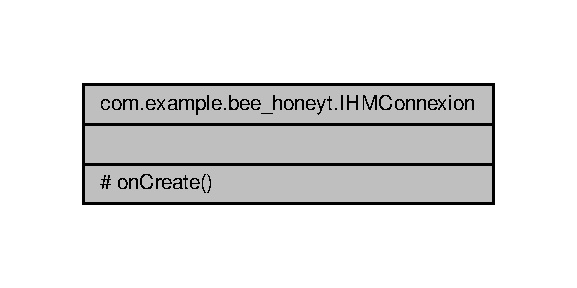
\includegraphics[width=277pt]{classcom_1_1example_1_1bee__honeyt_1_1_i_h_m_connexion__coll__graph}
\end{center}
\end{figure}
\subsubsection*{Fonctions membres protégées}
\begin{DoxyCompactItemize}
\item 
void \hyperlink{classcom_1_1example_1_1bee__honeyt_1_1_i_h_m_connexion_a4949c5484f6719c377d94a4a88143fb9}{on\+Create} (Bundle saved\+Instance\+State)
\end{DoxyCompactItemize}


\subsubsection{Description détaillée}


Définition à la ligne \hyperlink{_i_h_m_connexion_8java_source_l00015}{15} du fichier \hyperlink{_i_h_m_connexion_8java_source}{I\+H\+M\+Connexion.\+java}.



\subsubsection{Documentation des fonctions membres}
\mbox{\Hypertarget{classcom_1_1example_1_1bee__honeyt_1_1_i_h_m_connexion_a4949c5484f6719c377d94a4a88143fb9}\label{classcom_1_1example_1_1bee__honeyt_1_1_i_h_m_connexion_a4949c5484f6719c377d94a4a88143fb9}} 
\index{com\+::example\+::bee\+\_\+honeyt\+::\+I\+H\+M\+Connexion@{com\+::example\+::bee\+\_\+honeyt\+::\+I\+H\+M\+Connexion}!on\+Create@{on\+Create}}
\index{on\+Create@{on\+Create}!com\+::example\+::bee\+\_\+honeyt\+::\+I\+H\+M\+Connexion@{com\+::example\+::bee\+\_\+honeyt\+::\+I\+H\+M\+Connexion}}
\paragraph{\texorpdfstring{on\+Create()}{onCreate()}}
{\footnotesize\ttfamily void com.\+example.\+bee\+\_\+honeyt.\+I\+H\+M\+Connexion.\+on\+Create (\begin{DoxyParamCaption}\item[{Bundle}]{saved\+Instance\+State }\end{DoxyParamCaption})\hspace{0.3cm}{\ttfamily [protected]}}



Définition à la ligne \hyperlink{_i_h_m_connexion_8java_source_l00019}{19} du fichier \hyperlink{_i_h_m_connexion_8java_source}{I\+H\+M\+Connexion.\+java}.


\begin{DoxyCode}
00020     \{
00021         super.onCreate(savedInstanceState);
00022         setContentView(R.layout.activity\_ihm\_connexion);
00023     \}
\end{DoxyCode}


La documentation de cette classe a été générée à partir du fichier suivant \+:\begin{DoxyCompactItemize}
\item 
\hyperlink{_i_h_m_connexion_8java}{I\+H\+M\+Connexion.\+java}\end{DoxyCompactItemize}

\hypertarget{classcom_1_1example_1_1bee__honeyt_1_1_i_h_m_mobile}{}\subsection{Référence de la classe com.\+example.\+bee\+\_\+honeyt.\+I\+H\+M\+Mobile}
\label{classcom_1_1example_1_1bee__honeyt_1_1_i_h_m_mobile}\index{com.\+example.\+bee\+\_\+honeyt.\+I\+H\+M\+Mobile@{com.\+example.\+bee\+\_\+honeyt.\+I\+H\+M\+Mobile}}


L\textquotesingle{}activité principale de l\textquotesingle{}application Bee\+Honey\textquotesingle{}t.  




Graphe de collaboration de com.\+example.\+bee\+\_\+honeyt.\+I\+H\+M\+Mobile\+:
\nopagebreak
\begin{figure}[H]
\begin{center}
\leavevmode
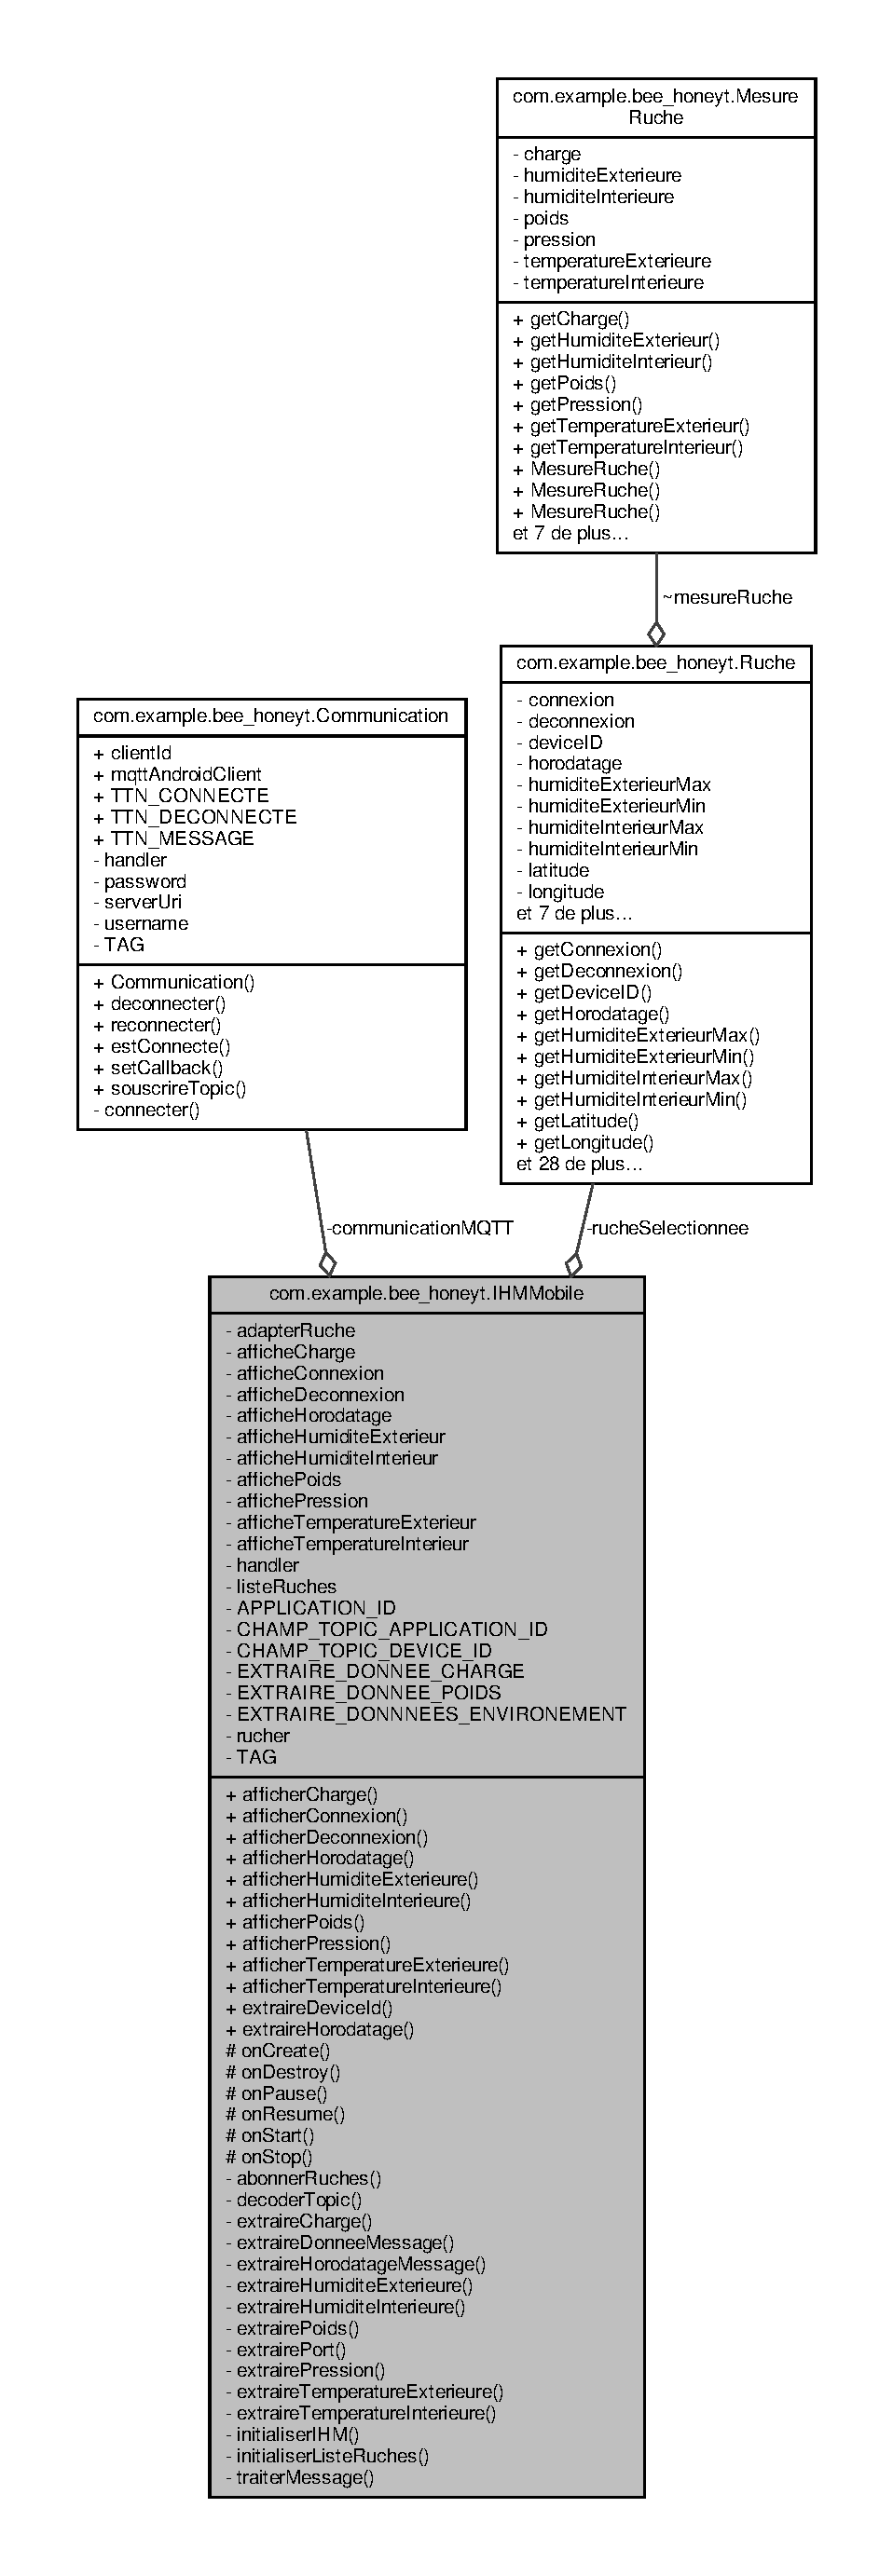
\includegraphics[height=550pt]{classcom_1_1example_1_1bee__honeyt_1_1_i_h_m_mobile__coll__graph}
\end{center}
\end{figure}
\subsubsection*{Fonctions membres publiques}
\begin{DoxyCompactItemize}
\item 
void \hyperlink{classcom_1_1example_1_1bee__honeyt_1_1_i_h_m_mobile_a64c55ee927d9cb31265989d0296edc53}{afficher\+Charge} (int charge)
\begin{DoxyCompactList}\small\item\em Affiche la charge. \end{DoxyCompactList}\item 
void \hyperlink{classcom_1_1example_1_1bee__honeyt_1_1_i_h_m_mobile_a09149878e7ab1c24fa1b3aea037bd3fc}{afficher\+Connexion} (String connexion)
\begin{DoxyCompactList}\small\item\em Affiche la connexion au topic. \end{DoxyCompactList}\item 
void \hyperlink{classcom_1_1example_1_1bee__honeyt_1_1_i_h_m_mobile_a8eeb63d847d450223c641107e2f27f1a}{afficher\+Deconnexion} (String deconnexion)
\item 
void \hyperlink{classcom_1_1example_1_1bee__honeyt_1_1_i_h_m_mobile_ae1a488c4774eea0b794257f576ab932d}{afficher\+Horodatage} (String horodatage)
\begin{DoxyCompactList}\small\item\em Affiche l\textquotesingle{}horodatage. \end{DoxyCompactList}\item 
void \hyperlink{classcom_1_1example_1_1bee__honeyt_1_1_i_h_m_mobile_a8571df97f453ee83c35d653b06127691}{afficher\+Humidite\+Exterieure} (int humidite\+Exterieure)
\begin{DoxyCompactList}\small\item\em Affiche l\textquotesingle{}humidite exterieure. \end{DoxyCompactList}\item 
void \hyperlink{classcom_1_1example_1_1bee__honeyt_1_1_i_h_m_mobile_ae59dbfdcd0be7d98bb714398931028b5}{afficher\+Humidite\+Interieure} (int humidite\+Interieure)
\begin{DoxyCompactList}\small\item\em Affiche l\textquotesingle{}humidite interieure. \end{DoxyCompactList}\item 
void \hyperlink{classcom_1_1example_1_1bee__honeyt_1_1_i_h_m_mobile_a2f4fe6cded3a35b0152e43d546be5565}{afficher\+Poids} (double poids)
\begin{DoxyCompactList}\small\item\em Affiche le poids. \end{DoxyCompactList}\item 
void \hyperlink{classcom_1_1example_1_1bee__honeyt_1_1_i_h_m_mobile_a92bb00501214f2f5f9805a005f1ecdaa}{afficher\+Pression} (int pression)
\begin{DoxyCompactList}\small\item\em Affiche la pression. \end{DoxyCompactList}\item 
void \hyperlink{classcom_1_1example_1_1bee__honeyt_1_1_i_h_m_mobile_af7ce50e9cc663c2c9198bbbb2b7882ff}{afficher\+Temperature\+Exterieure} (double temperature\+Exterieure)
\begin{DoxyCompactList}\small\item\em Affiche la température exterieure. \end{DoxyCompactList}\item 
void \hyperlink{classcom_1_1example_1_1bee__honeyt_1_1_i_h_m_mobile_ac0f55897a183a0887c87954f6fbfdf2f}{afficher\+Temperature\+Interieure} (double temperature\+Interieure)
\begin{DoxyCompactList}\small\item\em Affiche la température intérieure. \end{DoxyCompactList}\item 
String \hyperlink{classcom_1_1example_1_1bee__honeyt_1_1_i_h_m_mobile_ab957cc8fd25c104c48341f7e4141e173}{extraire\+Device\+Id} (String topic)
\item 
String \hyperlink{classcom_1_1example_1_1bee__honeyt_1_1_i_h_m_mobile_ae14deb90573474bc46817312624ebd20}{extraire\+Horodatage} (String meta\+Data)
\end{DoxyCompactItemize}
\subsubsection*{Fonctions membres protégées}
\begin{DoxyCompactItemize}
\item 
void \hyperlink{classcom_1_1example_1_1bee__honeyt_1_1_i_h_m_mobile_af487b0250bfc0e873fe3a4f495c3ef5e}{on\+Create} (Bundle saved\+Instance\+State)
\begin{DoxyCompactList}\small\item\em Méthode appelée à la création de l\textquotesingle{}application. \end{DoxyCompactList}\item 
void \hyperlink{classcom_1_1example_1_1bee__honeyt_1_1_i_h_m_mobile_a35ee33d6497d0ed0a5acacefaebce63a}{on\+Destroy} ()
\begin{DoxyCompactList}\small\item\em Méthode appelée à la destruction de l\textquotesingle{}application (après \hyperlink{classcom_1_1example_1_1bee__honeyt_1_1_i_h_m_mobile_ad341d4dd8d326f2ecdca7a5447c3f8a4}{on\+Stop()} et détruite par le système Android) \end{DoxyCompactList}\item 
void \hyperlink{classcom_1_1example_1_1bee__honeyt_1_1_i_h_m_mobile_a8b2f247beaf4e5f146c579b38d8bdee9}{on\+Pause} ()
\begin{DoxyCompactList}\small\item\em Méthode appelée après qu\textquotesingle{}une boîte de dialogue s\textquotesingle{}est affichée (on reprend sur un \hyperlink{classcom_1_1example_1_1bee__honeyt_1_1_i_h_m_mobile_aa8e9489786f095aee58ae5895b118ef6}{on\+Resume()}) ou avant \hyperlink{classcom_1_1example_1_1bee__honeyt_1_1_i_h_m_mobile_ad341d4dd8d326f2ecdca7a5447c3f8a4}{on\+Stop()} (activité plus visible) \end{DoxyCompactList}\item 
void \hyperlink{classcom_1_1example_1_1bee__honeyt_1_1_i_h_m_mobile_aa8e9489786f095aee58ae5895b118ef6}{on\+Resume} ()
\begin{DoxyCompactList}\small\item\em Méthode appelée après \hyperlink{classcom_1_1example_1_1bee__honeyt_1_1_i_h_m_mobile_abab25414f97d4793152b39c2deb8365b}{on\+Start()} ou après \hyperlink{classcom_1_1example_1_1bee__honeyt_1_1_i_h_m_mobile_a8b2f247beaf4e5f146c579b38d8bdee9}{on\+Pause()} \end{DoxyCompactList}\item 
void \hyperlink{classcom_1_1example_1_1bee__honeyt_1_1_i_h_m_mobile_abab25414f97d4793152b39c2deb8365b}{on\+Start} ()
\begin{DoxyCompactList}\small\item\em Méthode appelée au démarrage après le \hyperlink{classcom_1_1example_1_1bee__honeyt_1_1_i_h_m_mobile_af487b0250bfc0e873fe3a4f495c3ef5e}{on\+Create()} ou un restart après un \hyperlink{classcom_1_1example_1_1bee__honeyt_1_1_i_h_m_mobile_ad341d4dd8d326f2ecdca7a5447c3f8a4}{on\+Stop()} \end{DoxyCompactList}\item 
void \hyperlink{classcom_1_1example_1_1bee__honeyt_1_1_i_h_m_mobile_ad341d4dd8d326f2ecdca7a5447c3f8a4}{on\+Stop} ()
\begin{DoxyCompactList}\small\item\em Méthode appelée lorsque l\textquotesingle{}activité n\textquotesingle{}est plus visible. \end{DoxyCompactList}\end{DoxyCompactItemize}
\subsubsection*{Fonctions membres privées}
\begin{DoxyCompactItemize}
\item 
void \hyperlink{classcom_1_1example_1_1bee__honeyt_1_1_i_h_m_mobile_ac255143b5796de6ee0be9852d2b89396}{abonner\+Ruches} ()
\item 
void \hyperlink{classcom_1_1example_1_1bee__honeyt_1_1_i_h_m_mobile_a7bc9099049f98bcc154c1e8d9f773133}{decoder\+Topic} (String topic)
\item 
int \hyperlink{classcom_1_1example_1_1bee__honeyt_1_1_i_h_m_mobile_a1c9c8df9039fc494293b40011ddf6f5e}{extraire\+Charge} (String payload\+Fields)
\item 
String \hyperlink{classcom_1_1example_1_1bee__honeyt_1_1_i_h_m_mobile_a2f781039138b814510102847e70917a1}{extraire\+Donnee\+Message} (String message)
\item 
String \hyperlink{classcom_1_1example_1_1bee__honeyt_1_1_i_h_m_mobile_aabe15decc02b7f56a82f60dac75f8c2f}{extraire\+Horodatage\+Message} (String message)
\item 
int \hyperlink{classcom_1_1example_1_1bee__honeyt_1_1_i_h_m_mobile_a9a8131f2198266585e602e6fe9d29ef0}{extraire\+Humidite\+Exterieure} (String payload\+Fields)
\item 
int \hyperlink{classcom_1_1example_1_1bee__honeyt_1_1_i_h_m_mobile_afb44a51a66e904c2b3e5229ab5144f56}{extraire\+Humidite\+Interieure} (String payload\+Fields)
\item 
double \hyperlink{classcom_1_1example_1_1bee__honeyt_1_1_i_h_m_mobile_ad702e818ba1d861f26accfd6a0194b86}{extraire\+Poids} (String payload\+Fields)
\item 
int \hyperlink{classcom_1_1example_1_1bee__honeyt_1_1_i_h_m_mobile_abc4571bc8b1400c6d75c0a2594b0abe6}{extraire\+Port} (String message)
\item 
int \hyperlink{classcom_1_1example_1_1bee__honeyt_1_1_i_h_m_mobile_ad49ff3588da89162f21ca8e983a0fb4c}{extraire\+Pression} (String payload\+Fields)
\item 
double \hyperlink{classcom_1_1example_1_1bee__honeyt_1_1_i_h_m_mobile_a80b9ad15fb6aa3591cf600892b1325b9}{extraire\+Temperature\+Exterieure} (String payload\+Fields)
\item 
double \hyperlink{classcom_1_1example_1_1bee__honeyt_1_1_i_h_m_mobile_a714f52f4793f22a08a773b1bf35dd015}{extraire\+Temperature\+Interieure} (String payload\+Fields)
\item 
void \hyperlink{classcom_1_1example_1_1bee__honeyt_1_1_i_h_m_mobile_a4aa9d23a3aebf2d1a3cd62a15a4e0f2d}{initialiser\+I\+HM} ()
\begin{DoxyCompactList}\small\item\em Méthode pour initialiser l\textquotesingle{}I\+HM. \end{DoxyCompactList}\item 
void \hyperlink{classcom_1_1example_1_1bee__honeyt_1_1_i_h_m_mobile_a1fb171bee5ff2ce052ad88fb9bc84718}{initialiser\+Liste\+Ruches} ()
\begin{DoxyCompactList}\small\item\em Initialise la liste déroulante des ruches. \end{DoxyCompactList}\item 
void \hyperlink{classcom_1_1example_1_1bee__honeyt_1_1_i_h_m_mobile_a4183e896e4eab05e7ca92735199425fa}{traiter\+Message} (String message)
\end{DoxyCompactItemize}
\subsubsection*{Attributs privés}
\begin{DoxyCompactItemize}
\item 
Array\+Adapter$<$ String $>$ \hyperlink{classcom_1_1example_1_1bee__honeyt_1_1_i_h_m_mobile_afafe74da6dfeae76058bfbf17d4d23b3}{adapter\+Ruche}
\begin{DoxyCompactList}\small\item\em Adaptateur pour mettre la liste de noms de ruche. \end{DoxyCompactList}\item 
Text\+View \hyperlink{classcom_1_1example_1_1bee__honeyt_1_1_i_h_m_mobile_af83151ec51b1f533802cf95057667215}{affiche\+Charge}
\item 
Text\+View \hyperlink{classcom_1_1example_1_1bee__honeyt_1_1_i_h_m_mobile_af2248fbfeeed19f1256db84bf3a4dc94}{affiche\+Connexion}
\item 
Text\+View \hyperlink{classcom_1_1example_1_1bee__honeyt_1_1_i_h_m_mobile_a6387ccc4e8483220e821e9e88f7d3964}{affiche\+Deconnexion}
\item 
Text\+View \hyperlink{classcom_1_1example_1_1bee__honeyt_1_1_i_h_m_mobile_a624f148d43715aa48ba84e749637c2a5}{affiche\+Horodatage}
\item 
Text\+View \hyperlink{classcom_1_1example_1_1bee__honeyt_1_1_i_h_m_mobile_aa75e62918ab5b0322199d3a9919de17b}{affiche\+Humidite\+Exterieur}
\item 
Text\+View \hyperlink{classcom_1_1example_1_1bee__honeyt_1_1_i_h_m_mobile_af061affda51e77bec2c6850b3895dc76}{affiche\+Humidite\+Interieur}
\item 
Text\+View \hyperlink{classcom_1_1example_1_1bee__honeyt_1_1_i_h_m_mobile_a83854ea1a388eb4919c953ef00e8fa7f}{affiche\+Poids}
\item 
Text\+View \hyperlink{classcom_1_1example_1_1bee__honeyt_1_1_i_h_m_mobile_a2bc1237c9f17c51c2f506c31fba5b264}{affiche\+Pression}
\item 
Text\+View \hyperlink{classcom_1_1example_1_1bee__honeyt_1_1_i_h_m_mobile_a102530688eabbb8bfa549291b51a78ba}{affiche\+Temperature\+Exterieur}
\item 
Text\+View \hyperlink{classcom_1_1example_1_1bee__honeyt_1_1_i_h_m_mobile_ac553e3089f95a9fec9ec7345ad3aefcd}{affiche\+Temperature\+Interieur}
\item 
\hyperlink{classcom_1_1example_1_1bee__honeyt_1_1_communication}{Communication} \hyperlink{classcom_1_1example_1_1bee__honeyt_1_1_i_h_m_mobile_a832529dab7bfae5405c5496e971e8c84}{communication\+M\+Q\+TT}
\item 
final Handler \hyperlink{classcom_1_1example_1_1bee__honeyt_1_1_i_h_m_mobile_ab04ad38c9ee9a2621cb1b10cc2da1df2}{handler}
\begin{DoxyCompactList}\small\item\em Handler de communication entre l\textquotesingle{}activité et la communication M\+Q\+TT. \end{DoxyCompactList}\item 
Spinner \hyperlink{classcom_1_1example_1_1bee__honeyt_1_1_i_h_m_mobile_a7275bce8e0026b1043371e6878ff65c1}{liste\+Ruches}
\begin{DoxyCompactList}\small\item\em Liste déroulante pour les ruches. \end{DoxyCompactList}\item 
\hyperlink{classcom_1_1example_1_1bee__honeyt_1_1_ruche}{Ruche} \hyperlink{classcom_1_1example_1_1bee__honeyt_1_1_i_h_m_mobile_af59d4b185d3931df2e98568e99673778}{ruche\+Selectionnee}
\end{DoxyCompactItemize}
\subsubsection*{Attributs privés statiques}
\begin{DoxyCompactItemize}
\item 
static final String \hyperlink{classcom_1_1example_1_1bee__honeyt_1_1_i_h_m_mobile_a92fe694fa515e68960a0add6212b2e86}{A\+P\+P\+L\+I\+C\+A\+T\+I\+O\+N\+\_\+\+ID} = \char`\"{}rucher\char`\"{}
\item 
static final int \hyperlink{classcom_1_1example_1_1bee__honeyt_1_1_i_h_m_mobile_aa49d99fb22c1f7d014bfb60d1d322fc6}{C\+H\+A\+M\+P\+\_\+\+T\+O\+P\+I\+C\+\_\+\+A\+P\+P\+L\+I\+C\+A\+T\+I\+O\+N\+\_\+\+ID} = 0
\item 
static final int \hyperlink{classcom_1_1example_1_1bee__honeyt_1_1_i_h_m_mobile_ac6703593d2a2d227d51c89b8185060fc}{C\+H\+A\+M\+P\+\_\+\+T\+O\+P\+I\+C\+\_\+\+D\+E\+V\+I\+C\+E\+\_\+\+ID} = 1
\item 
static final int \hyperlink{classcom_1_1example_1_1bee__honeyt_1_1_i_h_m_mobile_a5cc87519c4cba4d1f16dd98e300487a2}{E\+X\+T\+R\+A\+I\+R\+E\+\_\+\+D\+O\+N\+N\+E\+E\+\_\+\+C\+H\+A\+R\+GE} = 3
\item 
static final int \hyperlink{classcom_1_1example_1_1bee__honeyt_1_1_i_h_m_mobile_a2e9be0481d1498b9883b92bcb4d51619}{E\+X\+T\+R\+A\+I\+R\+E\+\_\+\+D\+O\+N\+N\+E\+E\+\_\+\+P\+O\+I\+DS} = 1
\item 
static final int \hyperlink{classcom_1_1example_1_1bee__honeyt_1_1_i_h_m_mobile_aea71e02f7d7a9a5767821ba3803bdd80}{E\+X\+T\+R\+A\+I\+R\+E\+\_\+\+D\+O\+N\+N\+N\+E\+E\+S\+\_\+\+E\+N\+V\+I\+R\+O\+N\+E\+M\+E\+NT} = 2
\item 
static Vector$<$ \hyperlink{classcom_1_1example_1_1bee__honeyt_1_1_ruche}{Ruche} $>$ \hyperlink{classcom_1_1example_1_1bee__honeyt_1_1_i_h_m_mobile_a80b422d45e9b5c91f7bcad1dca4ad292}{rucher}
\begin{DoxyCompactList}\small\item\em Conteneur pour les ruches. \end{DoxyCompactList}\item 
static final String \hyperlink{classcom_1_1example_1_1bee__honeyt_1_1_i_h_m_mobile_a366987bf9bb2ed1010b2f967d4efa263}{T\+AG} = \char`\"{}\+\_\+\+I\+H\+M\+Mobile\char`\"{}
\begin{DoxyCompactList}\small\item\em T\+AG pour les logs. \end{DoxyCompactList}\end{DoxyCompactItemize}


\subsubsection{Description détaillée}
L\textquotesingle{}activité principale de l\textquotesingle{}application Bee\+Honey\textquotesingle{}t. 

Définition à la ligne \hyperlink{_i_h_m_mobile_8java_source_l00043}{43} du fichier \hyperlink{_i_h_m_mobile_8java_source}{I\+H\+M\+Mobile.\+java}.



\subsubsection{Documentation des fonctions membres}
\mbox{\Hypertarget{classcom_1_1example_1_1bee__honeyt_1_1_i_h_m_mobile_ac255143b5796de6ee0be9852d2b89396}\label{classcom_1_1example_1_1bee__honeyt_1_1_i_h_m_mobile_ac255143b5796de6ee0be9852d2b89396}} 
\index{com\+::example\+::bee\+\_\+honeyt\+::\+I\+H\+M\+Mobile@{com\+::example\+::bee\+\_\+honeyt\+::\+I\+H\+M\+Mobile}!abonner\+Ruches@{abonner\+Ruches}}
\index{abonner\+Ruches@{abonner\+Ruches}!com\+::example\+::bee\+\_\+honeyt\+::\+I\+H\+M\+Mobile@{com\+::example\+::bee\+\_\+honeyt\+::\+I\+H\+M\+Mobile}}
\paragraph{\texorpdfstring{abonner\+Ruches()}{abonnerRuches()}}
{\footnotesize\ttfamily void com.\+example.\+bee\+\_\+honeyt.\+I\+H\+M\+Mobile.\+abonner\+Ruches (\begin{DoxyParamCaption}{ }\end{DoxyParamCaption})\hspace{0.3cm}{\ttfamily [private]}}



Définition à la ligne \hyperlink{_i_h_m_mobile_8java_source_l00563}{563} du fichier \hyperlink{_i_h_m_mobile_8java_source}{I\+H\+M\+Mobile.\+java}.



Références \hyperlink{_communication_8java_source_l00232}{com.\+example.\+bee\+\_\+honeyt.\+Communication.\+souscrire\+Topic()}.


\begin{DoxyCode}
00564     \{
00565         \textcolor{comment}{// Abonner les ruches pour recevoir les données}
00566         \textcolor{keywordflow}{for} (\textcolor{keywordtype}{int} i = 0; i < \hyperlink{classcom_1_1example_1_1bee__honeyt_1_1_i_h_m_mobile_a80b422d45e9b5c91f7bcad1dca4ad292}{rucher}.size(); i++)
00567         \{
00568             \hyperlink{classcom_1_1example_1_1bee__honeyt_1_1_i_h_m_mobile_a832529dab7bfae5405c5496e971e8c84}{communicationMQTT}.\hyperlink{classcom_1_1example_1_1bee__honeyt_1_1_communication_aa1093a3d4f3479595a36ef2425f3ef70}{souscrireTopic}(
      \hyperlink{classcom_1_1example_1_1bee__honeyt_1_1_i_h_m_mobile_a80b422d45e9b5c91f7bcad1dca4ad292}{rucher}.get(i).getDeviceID());
00569         \}
00570     \}
\end{DoxyCode}
\mbox{\Hypertarget{classcom_1_1example_1_1bee__honeyt_1_1_i_h_m_mobile_a64c55ee927d9cb31265989d0296edc53}\label{classcom_1_1example_1_1bee__honeyt_1_1_i_h_m_mobile_a64c55ee927d9cb31265989d0296edc53}} 
\index{com\+::example\+::bee\+\_\+honeyt\+::\+I\+H\+M\+Mobile@{com\+::example\+::bee\+\_\+honeyt\+::\+I\+H\+M\+Mobile}!afficher\+Charge@{afficher\+Charge}}
\index{afficher\+Charge@{afficher\+Charge}!com\+::example\+::bee\+\_\+honeyt\+::\+I\+H\+M\+Mobile@{com\+::example\+::bee\+\_\+honeyt\+::\+I\+H\+M\+Mobile}}
\paragraph{\texorpdfstring{afficher\+Charge()}{afficherCharge()}}
{\footnotesize\ttfamily void com.\+example.\+bee\+\_\+honeyt.\+I\+H\+M\+Mobile.\+afficher\+Charge (\begin{DoxyParamCaption}\item[{int}]{charge }\end{DoxyParamCaption})}



Affiche la charge. 


\begin{DoxyParams}{Paramètres}
{\em charge} & la charge en Kg \\
\hline
\end{DoxyParams}


Définition à la ligne \hyperlink{_i_h_m_mobile_8java_source_l00289}{289} du fichier \hyperlink{_i_h_m_mobile_8java_source}{I\+H\+M\+Mobile.\+java}.



Référencé par \hyperlink{_i_h_m_mobile_8java_source_l00152}{com.\+example.\+bee\+\_\+honeyt.\+I\+H\+M\+Mobile.\+initialiser\+I\+H\+M()}, \hyperlink{_i_h_m_mobile_8java_source_l00170}{com.\+example.\+bee\+\_\+honeyt.\+I\+H\+M\+Mobile.\+initialiser\+Liste\+Ruches()}, et \hyperlink{_i_h_m_mobile_8java_source_l00374}{com.\+example.\+bee\+\_\+honeyt.\+I\+H\+M\+Mobile.\+traiter\+Message()}.


\begin{DoxyCode}
00290     \{
00291         \hyperlink{classcom_1_1example_1_1bee__honeyt_1_1_i_h_m_mobile_af83151ec51b1f533802cf95057667215}{afficheCharge} = (TextView) findViewById(R.id.afficheCharge);
00292         \hyperlink{classcom_1_1example_1_1bee__honeyt_1_1_i_h_m_mobile_af83151ec51b1f533802cf95057667215}{afficheCharge}.setText(\textcolor{stringliteral}{"Charge : "} + charge  + \textcolor{stringliteral}{" %"});
00293     \}
\end{DoxyCode}
\mbox{\Hypertarget{classcom_1_1example_1_1bee__honeyt_1_1_i_h_m_mobile_a09149878e7ab1c24fa1b3aea037bd3fc}\label{classcom_1_1example_1_1bee__honeyt_1_1_i_h_m_mobile_a09149878e7ab1c24fa1b3aea037bd3fc}} 
\index{com\+::example\+::bee\+\_\+honeyt\+::\+I\+H\+M\+Mobile@{com\+::example\+::bee\+\_\+honeyt\+::\+I\+H\+M\+Mobile}!afficher\+Connexion@{afficher\+Connexion}}
\index{afficher\+Connexion@{afficher\+Connexion}!com\+::example\+::bee\+\_\+honeyt\+::\+I\+H\+M\+Mobile@{com\+::example\+::bee\+\_\+honeyt\+::\+I\+H\+M\+Mobile}}
\paragraph{\texorpdfstring{afficher\+Connexion()}{afficherConnexion()}}
{\footnotesize\ttfamily void com.\+example.\+bee\+\_\+honeyt.\+I\+H\+M\+Mobile.\+afficher\+Connexion (\begin{DoxyParamCaption}\item[{String}]{connexion }\end{DoxyParamCaption})}



Affiche la connexion au topic. 



Définition à la ligne \hyperlink{_i_h_m_mobile_8java_source_l00306}{306} du fichier \hyperlink{_i_h_m_mobile_8java_source}{I\+H\+M\+Mobile.\+java}.


\begin{DoxyCode}
00307     \{
00308         connexion = \textcolor{stringliteral}{"Connecté"};
00309         \hyperlink{classcom_1_1example_1_1bee__honeyt_1_1_i_h_m_mobile_af2248fbfeeed19f1256db84bf3a4dc94}{afficheConnexion} = (TextView) findViewById(R.id.afficheConnexion);
00310         \hyperlink{classcom_1_1example_1_1bee__honeyt_1_1_i_h_m_mobile_af2248fbfeeed19f1256db84bf3a4dc94}{afficheConnexion}.setText(connexion);
00311     \}
\end{DoxyCode}
\mbox{\Hypertarget{classcom_1_1example_1_1bee__honeyt_1_1_i_h_m_mobile_a8eeb63d847d450223c641107e2f27f1a}\label{classcom_1_1example_1_1bee__honeyt_1_1_i_h_m_mobile_a8eeb63d847d450223c641107e2f27f1a}} 
\index{com\+::example\+::bee\+\_\+honeyt\+::\+I\+H\+M\+Mobile@{com\+::example\+::bee\+\_\+honeyt\+::\+I\+H\+M\+Mobile}!afficher\+Deconnexion@{afficher\+Deconnexion}}
\index{afficher\+Deconnexion@{afficher\+Deconnexion}!com\+::example\+::bee\+\_\+honeyt\+::\+I\+H\+M\+Mobile@{com\+::example\+::bee\+\_\+honeyt\+::\+I\+H\+M\+Mobile}}
\paragraph{\texorpdfstring{afficher\+Deconnexion()}{afficherDeconnexion()}}
{\footnotesize\ttfamily void com.\+example.\+bee\+\_\+honeyt.\+I\+H\+M\+Mobile.\+afficher\+Deconnexion (\begin{DoxyParamCaption}\item[{String}]{deconnexion }\end{DoxyParamCaption})}



Définition à la ligne \hyperlink{_i_h_m_mobile_8java_source_l00313}{313} du fichier \hyperlink{_i_h_m_mobile_8java_source}{I\+H\+M\+Mobile.\+java}.


\begin{DoxyCode}
00314     \{
00315         deconnexion = \textcolor{stringliteral}{"Deconnecté"};
00316         \hyperlink{classcom_1_1example_1_1bee__honeyt_1_1_i_h_m_mobile_a6387ccc4e8483220e821e9e88f7d3964}{afficheDeconnexion} = (TextView) findViewById(R.id.afficheDeconnexion);
00317         \hyperlink{classcom_1_1example_1_1bee__honeyt_1_1_i_h_m_mobile_a6387ccc4e8483220e821e9e88f7d3964}{afficheDeconnexion}.setText(deconnexion);
00318     \}
\end{DoxyCode}
\mbox{\Hypertarget{classcom_1_1example_1_1bee__honeyt_1_1_i_h_m_mobile_ae1a488c4774eea0b794257f576ab932d}\label{classcom_1_1example_1_1bee__honeyt_1_1_i_h_m_mobile_ae1a488c4774eea0b794257f576ab932d}} 
\index{com\+::example\+::bee\+\_\+honeyt\+::\+I\+H\+M\+Mobile@{com\+::example\+::bee\+\_\+honeyt\+::\+I\+H\+M\+Mobile}!afficher\+Horodatage@{afficher\+Horodatage}}
\index{afficher\+Horodatage@{afficher\+Horodatage}!com\+::example\+::bee\+\_\+honeyt\+::\+I\+H\+M\+Mobile@{com\+::example\+::bee\+\_\+honeyt\+::\+I\+H\+M\+Mobile}}
\paragraph{\texorpdfstring{afficher\+Horodatage()}{afficherHorodatage()}}
{\footnotesize\ttfamily void com.\+example.\+bee\+\_\+honeyt.\+I\+H\+M\+Mobile.\+afficher\+Horodatage (\begin{DoxyParamCaption}\item[{String}]{horodatage }\end{DoxyParamCaption})}



Affiche l\textquotesingle{}horodatage. 


\begin{DoxyParams}{Paramètres}
{\em horodatage} & l\textquotesingle{}horodatage en J\+J/\+M\+M/\+AA + l\textquotesingle{}heure \\
\hline
\end{DoxyParams}


Définition à la ligne \hyperlink{_i_h_m_mobile_8java_source_l00298}{298} du fichier \hyperlink{_i_h_m_mobile_8java_source}{I\+H\+M\+Mobile.\+java}.



Référencé par \hyperlink{_i_h_m_mobile_8java_source_l00152}{com.\+example.\+bee\+\_\+honeyt.\+I\+H\+M\+Mobile.\+initialiser\+I\+H\+M()}, \hyperlink{_i_h_m_mobile_8java_source_l00170}{com.\+example.\+bee\+\_\+honeyt.\+I\+H\+M\+Mobile.\+initialiser\+Liste\+Ruches()}, et \hyperlink{_i_h_m_mobile_8java_source_l00374}{com.\+example.\+bee\+\_\+honeyt.\+I\+H\+M\+Mobile.\+traiter\+Message()}.


\begin{DoxyCode}
00299     \{
00300         \hyperlink{classcom_1_1example_1_1bee__honeyt_1_1_i_h_m_mobile_a624f148d43715aa48ba84e749637c2a5}{afficheHorodatage} = (TextView) findViewById(R.id.afficheHorodatage);
00301         \hyperlink{classcom_1_1example_1_1bee__honeyt_1_1_i_h_m_mobile_a624f148d43715aa48ba84e749637c2a5}{afficheHorodatage}.setText(horodatage);
00302     \}
\end{DoxyCode}
\mbox{\Hypertarget{classcom_1_1example_1_1bee__honeyt_1_1_i_h_m_mobile_a8571df97f453ee83c35d653b06127691}\label{classcom_1_1example_1_1bee__honeyt_1_1_i_h_m_mobile_a8571df97f453ee83c35d653b06127691}} 
\index{com\+::example\+::bee\+\_\+honeyt\+::\+I\+H\+M\+Mobile@{com\+::example\+::bee\+\_\+honeyt\+::\+I\+H\+M\+Mobile}!afficher\+Humidite\+Exterieure@{afficher\+Humidite\+Exterieure}}
\index{afficher\+Humidite\+Exterieure@{afficher\+Humidite\+Exterieure}!com\+::example\+::bee\+\_\+honeyt\+::\+I\+H\+M\+Mobile@{com\+::example\+::bee\+\_\+honeyt\+::\+I\+H\+M\+Mobile}}
\paragraph{\texorpdfstring{afficher\+Humidite\+Exterieure()}{afficherHumiditeExterieure()}}
{\footnotesize\ttfamily void com.\+example.\+bee\+\_\+honeyt.\+I\+H\+M\+Mobile.\+afficher\+Humidite\+Exterieure (\begin{DoxyParamCaption}\item[{int}]{humidite\+Exterieure }\end{DoxyParamCaption})}



Affiche l\textquotesingle{}humidite exterieure. 


\begin{DoxyParams}{Paramètres}
{\em humidite\+Exterieure} & l\textquotesingle{}humidite exterieure en \% \\
\hline
\end{DoxyParams}


Définition à la ligne \hyperlink{_i_h_m_mobile_8java_source_l00262}{262} du fichier \hyperlink{_i_h_m_mobile_8java_source}{I\+H\+M\+Mobile.\+java}.



Référencé par \hyperlink{_i_h_m_mobile_8java_source_l00152}{com.\+example.\+bee\+\_\+honeyt.\+I\+H\+M\+Mobile.\+initialiser\+I\+H\+M()}, \hyperlink{_i_h_m_mobile_8java_source_l00170}{com.\+example.\+bee\+\_\+honeyt.\+I\+H\+M\+Mobile.\+initialiser\+Liste\+Ruches()}, et \hyperlink{_i_h_m_mobile_8java_source_l00374}{com.\+example.\+bee\+\_\+honeyt.\+I\+H\+M\+Mobile.\+traiter\+Message()}.


\begin{DoxyCode}
00263     \{
00264         \hyperlink{classcom_1_1example_1_1bee__honeyt_1_1_i_h_m_mobile_aa75e62918ab5b0322199d3a9919de17b}{afficheHumiditeExterieur} = (TextView) findViewById(R.id.
      afficheHumiditeExterieur);
00265         \hyperlink{classcom_1_1example_1_1bee__honeyt_1_1_i_h_m_mobile_aa75e62918ab5b0322199d3a9919de17b}{afficheHumiditeExterieur}.setText(\textcolor{stringliteral}{"Humidité ext. : "} + humiditeExterieure + \textcolor{stringliteral}{
      " %"});
00266     \}
\end{DoxyCode}
\mbox{\Hypertarget{classcom_1_1example_1_1bee__honeyt_1_1_i_h_m_mobile_ae59dbfdcd0be7d98bb714398931028b5}\label{classcom_1_1example_1_1bee__honeyt_1_1_i_h_m_mobile_ae59dbfdcd0be7d98bb714398931028b5}} 
\index{com\+::example\+::bee\+\_\+honeyt\+::\+I\+H\+M\+Mobile@{com\+::example\+::bee\+\_\+honeyt\+::\+I\+H\+M\+Mobile}!afficher\+Humidite\+Interieure@{afficher\+Humidite\+Interieure}}
\index{afficher\+Humidite\+Interieure@{afficher\+Humidite\+Interieure}!com\+::example\+::bee\+\_\+honeyt\+::\+I\+H\+M\+Mobile@{com\+::example\+::bee\+\_\+honeyt\+::\+I\+H\+M\+Mobile}}
\paragraph{\texorpdfstring{afficher\+Humidite\+Interieure()}{afficherHumiditeInterieure()}}
{\footnotesize\ttfamily void com.\+example.\+bee\+\_\+honeyt.\+I\+H\+M\+Mobile.\+afficher\+Humidite\+Interieure (\begin{DoxyParamCaption}\item[{int}]{humidite\+Interieure }\end{DoxyParamCaption})}



Affiche l\textquotesingle{}humidite interieure. 


\begin{DoxyParams}{Paramètres}
{\em humidite\+Interieure} & l\textquotesingle{}humidite interieure en \% \\
\hline
\end{DoxyParams}


Définition à la ligne \hyperlink{_i_h_m_mobile_8java_source_l00253}{253} du fichier \hyperlink{_i_h_m_mobile_8java_source}{I\+H\+M\+Mobile.\+java}.



Référencé par \hyperlink{_i_h_m_mobile_8java_source_l00152}{com.\+example.\+bee\+\_\+honeyt.\+I\+H\+M\+Mobile.\+initialiser\+I\+H\+M()}, \hyperlink{_i_h_m_mobile_8java_source_l00170}{com.\+example.\+bee\+\_\+honeyt.\+I\+H\+M\+Mobile.\+initialiser\+Liste\+Ruches()}, et \hyperlink{_i_h_m_mobile_8java_source_l00374}{com.\+example.\+bee\+\_\+honeyt.\+I\+H\+M\+Mobile.\+traiter\+Message()}.


\begin{DoxyCode}
00254     \{
00255         \hyperlink{classcom_1_1example_1_1bee__honeyt_1_1_i_h_m_mobile_af061affda51e77bec2c6850b3895dc76}{afficheHumiditeInterieur} = (TextView) findViewById(R.id.
      afficheHumiditeInterieur);
00256         \hyperlink{classcom_1_1example_1_1bee__honeyt_1_1_i_h_m_mobile_af061affda51e77bec2c6850b3895dc76}{afficheHumiditeInterieur}.setText(\textcolor{stringliteral}{"Humidité int. : "} + humiditeInterieure + \textcolor{stringliteral}{
      " %"});
00257     \}
\end{DoxyCode}
\mbox{\Hypertarget{classcom_1_1example_1_1bee__honeyt_1_1_i_h_m_mobile_a2f4fe6cded3a35b0152e43d546be5565}\label{classcom_1_1example_1_1bee__honeyt_1_1_i_h_m_mobile_a2f4fe6cded3a35b0152e43d546be5565}} 
\index{com\+::example\+::bee\+\_\+honeyt\+::\+I\+H\+M\+Mobile@{com\+::example\+::bee\+\_\+honeyt\+::\+I\+H\+M\+Mobile}!afficher\+Poids@{afficher\+Poids}}
\index{afficher\+Poids@{afficher\+Poids}!com\+::example\+::bee\+\_\+honeyt\+::\+I\+H\+M\+Mobile@{com\+::example\+::bee\+\_\+honeyt\+::\+I\+H\+M\+Mobile}}
\paragraph{\texorpdfstring{afficher\+Poids()}{afficherPoids()}}
{\footnotesize\ttfamily void com.\+example.\+bee\+\_\+honeyt.\+I\+H\+M\+Mobile.\+afficher\+Poids (\begin{DoxyParamCaption}\item[{double}]{poids }\end{DoxyParamCaption})}



Affiche le poids. 


\begin{DoxyParams}{Paramètres}
{\em poids} & le poids en Kg \\
\hline
\end{DoxyParams}


Définition à la ligne \hyperlink{_i_h_m_mobile_8java_source_l00271}{271} du fichier \hyperlink{_i_h_m_mobile_8java_source}{I\+H\+M\+Mobile.\+java}.



Référencé par \hyperlink{_i_h_m_mobile_8java_source_l00152}{com.\+example.\+bee\+\_\+honeyt.\+I\+H\+M\+Mobile.\+initialiser\+I\+H\+M()}, \hyperlink{_i_h_m_mobile_8java_source_l00170}{com.\+example.\+bee\+\_\+honeyt.\+I\+H\+M\+Mobile.\+initialiser\+Liste\+Ruches()}, et \hyperlink{_i_h_m_mobile_8java_source_l00374}{com.\+example.\+bee\+\_\+honeyt.\+I\+H\+M\+Mobile.\+traiter\+Message()}.


\begin{DoxyCode}
00272     \{
00273         \hyperlink{classcom_1_1example_1_1bee__honeyt_1_1_i_h_m_mobile_a83854ea1a388eb4919c953ef00e8fa7f}{affichePoids} = (TextView) findViewById(R.id.affichePoids);
00274         \hyperlink{classcom_1_1example_1_1bee__honeyt_1_1_i_h_m_mobile_a83854ea1a388eb4919c953ef00e8fa7f}{affichePoids}.setText(\textcolor{stringliteral}{"Poids : "} + poids + \textcolor{stringliteral}{" Kg"});
00275     \}
\end{DoxyCode}
\mbox{\Hypertarget{classcom_1_1example_1_1bee__honeyt_1_1_i_h_m_mobile_a92bb00501214f2f5f9805a005f1ecdaa}\label{classcom_1_1example_1_1bee__honeyt_1_1_i_h_m_mobile_a92bb00501214f2f5f9805a005f1ecdaa}} 
\index{com\+::example\+::bee\+\_\+honeyt\+::\+I\+H\+M\+Mobile@{com\+::example\+::bee\+\_\+honeyt\+::\+I\+H\+M\+Mobile}!afficher\+Pression@{afficher\+Pression}}
\index{afficher\+Pression@{afficher\+Pression}!com\+::example\+::bee\+\_\+honeyt\+::\+I\+H\+M\+Mobile@{com\+::example\+::bee\+\_\+honeyt\+::\+I\+H\+M\+Mobile}}
\paragraph{\texorpdfstring{afficher\+Pression()}{afficherPression()}}
{\footnotesize\ttfamily void com.\+example.\+bee\+\_\+honeyt.\+I\+H\+M\+Mobile.\+afficher\+Pression (\begin{DoxyParamCaption}\item[{int}]{pression }\end{DoxyParamCaption})}



Affiche la pression. 


\begin{DoxyParams}{Paramètres}
{\em pression} & la pression en h\+PA \\
\hline
\end{DoxyParams}


Définition à la ligne \hyperlink{_i_h_m_mobile_8java_source_l00280}{280} du fichier \hyperlink{_i_h_m_mobile_8java_source}{I\+H\+M\+Mobile.\+java}.



Référencé par \hyperlink{_i_h_m_mobile_8java_source_l00152}{com.\+example.\+bee\+\_\+honeyt.\+I\+H\+M\+Mobile.\+initialiser\+I\+H\+M()}, \hyperlink{_i_h_m_mobile_8java_source_l00170}{com.\+example.\+bee\+\_\+honeyt.\+I\+H\+M\+Mobile.\+initialiser\+Liste\+Ruches()}, et \hyperlink{_i_h_m_mobile_8java_source_l00374}{com.\+example.\+bee\+\_\+honeyt.\+I\+H\+M\+Mobile.\+traiter\+Message()}.


\begin{DoxyCode}
00281     \{
00282         \hyperlink{classcom_1_1example_1_1bee__honeyt_1_1_i_h_m_mobile_a2bc1237c9f17c51c2f506c31fba5b264}{affichePression} = (TextView) findViewById(R.id.affichePression);
00283         \hyperlink{classcom_1_1example_1_1bee__honeyt_1_1_i_h_m_mobile_a2bc1237c9f17c51c2f506c31fba5b264}{affichePression}.setText(\textcolor{stringliteral}{"Pression : "} + pression  + \textcolor{stringliteral}{" hPa"});
00284     \}
\end{DoxyCode}
\mbox{\Hypertarget{classcom_1_1example_1_1bee__honeyt_1_1_i_h_m_mobile_af7ce50e9cc663c2c9198bbbb2b7882ff}\label{classcom_1_1example_1_1bee__honeyt_1_1_i_h_m_mobile_af7ce50e9cc663c2c9198bbbb2b7882ff}} 
\index{com\+::example\+::bee\+\_\+honeyt\+::\+I\+H\+M\+Mobile@{com\+::example\+::bee\+\_\+honeyt\+::\+I\+H\+M\+Mobile}!afficher\+Temperature\+Exterieure@{afficher\+Temperature\+Exterieure}}
\index{afficher\+Temperature\+Exterieure@{afficher\+Temperature\+Exterieure}!com\+::example\+::bee\+\_\+honeyt\+::\+I\+H\+M\+Mobile@{com\+::example\+::bee\+\_\+honeyt\+::\+I\+H\+M\+Mobile}}
\paragraph{\texorpdfstring{afficher\+Temperature\+Exterieure()}{afficherTemperatureExterieure()}}
{\footnotesize\ttfamily void com.\+example.\+bee\+\_\+honeyt.\+I\+H\+M\+Mobile.\+afficher\+Temperature\+Exterieure (\begin{DoxyParamCaption}\item[{double}]{temperature\+Exterieure }\end{DoxyParamCaption})}



Affiche la température exterieure. 


\begin{DoxyParams}{Paramètres}
{\em temperature\+Exterieure} & la température exterieure en °C \\
\hline
\end{DoxyParams}


Définition à la ligne \hyperlink{_i_h_m_mobile_8java_source_l00244}{244} du fichier \hyperlink{_i_h_m_mobile_8java_source}{I\+H\+M\+Mobile.\+java}.



Référencé par \hyperlink{_i_h_m_mobile_8java_source_l00152}{com.\+example.\+bee\+\_\+honeyt.\+I\+H\+M\+Mobile.\+initialiser\+I\+H\+M()}, \hyperlink{_i_h_m_mobile_8java_source_l00170}{com.\+example.\+bee\+\_\+honeyt.\+I\+H\+M\+Mobile.\+initialiser\+Liste\+Ruches()}, et \hyperlink{_i_h_m_mobile_8java_source_l00374}{com.\+example.\+bee\+\_\+honeyt.\+I\+H\+M\+Mobile.\+traiter\+Message()}.


\begin{DoxyCode}
00245     \{
00246         \hyperlink{classcom_1_1example_1_1bee__honeyt_1_1_i_h_m_mobile_a102530688eabbb8bfa549291b51a78ba}{afficheTemperatureExterieur} = (TextView) findViewById(R.id.
      afficheTemperatureExterieur);
00247         \hyperlink{classcom_1_1example_1_1bee__honeyt_1_1_i_h_m_mobile_a102530688eabbb8bfa549291b51a78ba}{afficheTemperatureExterieur}.setText(\textcolor{stringliteral}{"Température ext. : "} + 
      temperatureExterieure + \textcolor{stringliteral}{" °C"});
00248     \}
\end{DoxyCode}
\mbox{\Hypertarget{classcom_1_1example_1_1bee__honeyt_1_1_i_h_m_mobile_ac0f55897a183a0887c87954f6fbfdf2f}\label{classcom_1_1example_1_1bee__honeyt_1_1_i_h_m_mobile_ac0f55897a183a0887c87954f6fbfdf2f}} 
\index{com\+::example\+::bee\+\_\+honeyt\+::\+I\+H\+M\+Mobile@{com\+::example\+::bee\+\_\+honeyt\+::\+I\+H\+M\+Mobile}!afficher\+Temperature\+Interieure@{afficher\+Temperature\+Interieure}}
\index{afficher\+Temperature\+Interieure@{afficher\+Temperature\+Interieure}!com\+::example\+::bee\+\_\+honeyt\+::\+I\+H\+M\+Mobile@{com\+::example\+::bee\+\_\+honeyt\+::\+I\+H\+M\+Mobile}}
\paragraph{\texorpdfstring{afficher\+Temperature\+Interieure()}{afficherTemperatureInterieure()}}
{\footnotesize\ttfamily void com.\+example.\+bee\+\_\+honeyt.\+I\+H\+M\+Mobile.\+afficher\+Temperature\+Interieure (\begin{DoxyParamCaption}\item[{double}]{temperature\+Interieure }\end{DoxyParamCaption})}



Affiche la température intérieure. 


\begin{DoxyParams}{Paramètres}
{\em temperature\+Interieure} & la température intérieure en °C \\
\hline
\end{DoxyParams}


Définition à la ligne \hyperlink{_i_h_m_mobile_8java_source_l00235}{235} du fichier \hyperlink{_i_h_m_mobile_8java_source}{I\+H\+M\+Mobile.\+java}.



Référencé par \hyperlink{_i_h_m_mobile_8java_source_l00152}{com.\+example.\+bee\+\_\+honeyt.\+I\+H\+M\+Mobile.\+initialiser\+I\+H\+M()}, \hyperlink{_i_h_m_mobile_8java_source_l00170}{com.\+example.\+bee\+\_\+honeyt.\+I\+H\+M\+Mobile.\+initialiser\+Liste\+Ruches()}, et \hyperlink{_i_h_m_mobile_8java_source_l00374}{com.\+example.\+bee\+\_\+honeyt.\+I\+H\+M\+Mobile.\+traiter\+Message()}.


\begin{DoxyCode}
00236     \{
00237         \hyperlink{classcom_1_1example_1_1bee__honeyt_1_1_i_h_m_mobile_ac553e3089f95a9fec9ec7345ad3aefcd}{afficheTemperatureInterieur} = (TextView) findViewById(R.id.
      afficheTemperatureInterieur);
00238         \hyperlink{classcom_1_1example_1_1bee__honeyt_1_1_i_h_m_mobile_ac553e3089f95a9fec9ec7345ad3aefcd}{afficheTemperatureInterieur}.setText(\textcolor{stringliteral}{"Température int. : "} + 
      temperatureInterieure + \textcolor{stringliteral}{" °C"});
00239     \}
\end{DoxyCode}
\mbox{\Hypertarget{classcom_1_1example_1_1bee__honeyt_1_1_i_h_m_mobile_a7bc9099049f98bcc154c1e8d9f773133}\label{classcom_1_1example_1_1bee__honeyt_1_1_i_h_m_mobile_a7bc9099049f98bcc154c1e8d9f773133}} 
\index{com\+::example\+::bee\+\_\+honeyt\+::\+I\+H\+M\+Mobile@{com\+::example\+::bee\+\_\+honeyt\+::\+I\+H\+M\+Mobile}!decoder\+Topic@{decoder\+Topic}}
\index{decoder\+Topic@{decoder\+Topic}!com\+::example\+::bee\+\_\+honeyt\+::\+I\+H\+M\+Mobile@{com\+::example\+::bee\+\_\+honeyt\+::\+I\+H\+M\+Mobile}}
\paragraph{\texorpdfstring{decoder\+Topic()}{decoderTopic()}}
{\footnotesize\ttfamily void com.\+example.\+bee\+\_\+honeyt.\+I\+H\+M\+Mobile.\+decoder\+Topic (\begin{DoxyParamCaption}\item[{String}]{topic }\end{DoxyParamCaption})\hspace{0.3cm}{\ttfamily [private]}}

Exemple -\/$>$ topic = rucher/devices/ruche-\/2-\/sim/up \char`\"{}rucher\char`\"{} =$>$ Application\+ID \char`\"{}ruche-\/2-\/sim\char`\"{} =$>$ Device\+ID

Définition à la ligne \hyperlink{_i_h_m_mobile_8java_source_l00572}{572} du fichier \hyperlink{_i_h_m_mobile_8java_source}{I\+H\+M\+Mobile.\+java}.


\begin{DoxyCode}
00573     \{
00574         Log.d(\hyperlink{classcom_1_1example_1_1bee__honeyt_1_1_i_h_m_mobile_a366987bf9bb2ed1010b2f967d4efa263}{TAG}, \textcolor{stringliteral}{"extraireTopic() topic = "} + topic);
00580         \textcolor{keywordflow}{try}
00581         \{
00582             \textcolor{keywordflow}{if} (topic.startsWith(\hyperlink{classcom_1_1example_1_1bee__honeyt_1_1_i_h_m_mobile_a92fe694fa515e68960a0add6212b2e86}{APPLICATION\_ID}))
00583             \{
00584                 String[] champs = topic.split(\textcolor{stringliteral}{"/"});
00585 
00586                 \textcolor{keywordflow}{for} (\textcolor{keywordtype}{int} i = 0; i < champs.length; i++)
00587                 \{
00588                     Log.d(\hyperlink{classcom_1_1example_1_1bee__honeyt_1_1_i_h_m_mobile_a366987bf9bb2ed1010b2f967d4efa263}{TAG}, \textcolor{stringliteral}{"champs = "} + champs[i]);
00589                 \}
00590             \}
00591         \}
00592         \textcolor{keywordflow}{catch} (Exception e)
00593         \{
00594             e.printStackTrace();
00595         \}
00596     \}
\end{DoxyCode}
\mbox{\Hypertarget{classcom_1_1example_1_1bee__honeyt_1_1_i_h_m_mobile_a1c9c8df9039fc494293b40011ddf6f5e}\label{classcom_1_1example_1_1bee__honeyt_1_1_i_h_m_mobile_a1c9c8df9039fc494293b40011ddf6f5e}} 
\index{com\+::example\+::bee\+\_\+honeyt\+::\+I\+H\+M\+Mobile@{com\+::example\+::bee\+\_\+honeyt\+::\+I\+H\+M\+Mobile}!extraire\+Charge@{extraire\+Charge}}
\index{extraire\+Charge@{extraire\+Charge}!com\+::example\+::bee\+\_\+honeyt\+::\+I\+H\+M\+Mobile@{com\+::example\+::bee\+\_\+honeyt\+::\+I\+H\+M\+Mobile}}
\paragraph{\texorpdfstring{extraire\+Charge()}{extraireCharge()}}
{\footnotesize\ttfamily int com.\+example.\+bee\+\_\+honeyt.\+I\+H\+M\+Mobile.\+extraire\+Charge (\begin{DoxyParamCaption}\item[{String}]{payload\+Fields }\end{DoxyParamCaption})\hspace{0.3cm}{\ttfamily [private]}}



Définition à la ligne \hyperlink{_i_h_m_mobile_8java_source_l00739}{739} du fichier \hyperlink{_i_h_m_mobile_8java_source}{I\+H\+M\+Mobile.\+java}.



Référencé par \hyperlink{_i_h_m_mobile_8java_source_l00374}{com.\+example.\+bee\+\_\+honeyt.\+I\+H\+M\+Mobile.\+traiter\+Message()}.


\begin{DoxyCode}
00740     \{
00741         \textcolor{keywordtype}{int} charge = 0;
00742 
00743         \textcolor{keywordflow}{try}
00744         \{
00745             JSONObject json = null;
00746             Iterator<String> it = null;
00747             json = \textcolor{keyword}{new} JSONObject(payloadFields);
00748 
00749             charge = json.getInt(\textcolor{stringliteral}{"charge"});
00750             Log.d(\hyperlink{classcom_1_1example_1_1bee__honeyt_1_1_i_h_m_mobile_a366987bf9bb2ed1010b2f967d4efa263}{TAG}, \textcolor{stringliteral}{"extraireCharge() charge = "} + charge);
00751         \}
00752         \textcolor{keywordflow}{catch} (JSONException e)
00753         \{
00754             e.printStackTrace();
00755         \}
00756 
00757         \textcolor{keywordflow}{return} charge;
00758     \}
\end{DoxyCode}
\mbox{\Hypertarget{classcom_1_1example_1_1bee__honeyt_1_1_i_h_m_mobile_ab957cc8fd25c104c48341f7e4141e173}\label{classcom_1_1example_1_1bee__honeyt_1_1_i_h_m_mobile_ab957cc8fd25c104c48341f7e4141e173}} 
\index{com\+::example\+::bee\+\_\+honeyt\+::\+I\+H\+M\+Mobile@{com\+::example\+::bee\+\_\+honeyt\+::\+I\+H\+M\+Mobile}!extraire\+Device\+Id@{extraire\+Device\+Id}}
\index{extraire\+Device\+Id@{extraire\+Device\+Id}!com\+::example\+::bee\+\_\+honeyt\+::\+I\+H\+M\+Mobile@{com\+::example\+::bee\+\_\+honeyt\+::\+I\+H\+M\+Mobile}}
\paragraph{\texorpdfstring{extraire\+Device\+Id()}{extraireDeviceId()}}
{\footnotesize\ttfamily String com.\+example.\+bee\+\_\+honeyt.\+I\+H\+M\+Mobile.\+extraire\+Device\+Id (\begin{DoxyParamCaption}\item[{String}]{topic }\end{DoxyParamCaption})}



Définition à la ligne \hyperlink{_i_h_m_mobile_8java_source_l00720}{720} du fichier \hyperlink{_i_h_m_mobile_8java_source}{I\+H\+M\+Mobile.\+java}.


\begin{DoxyCode}
00721     \{
00722         Log.d(\hyperlink{classcom_1_1example_1_1bee__honeyt_1_1_i_h_m_mobile_a366987bf9bb2ed1010b2f967d4efa263}{TAG}, \textcolor{stringliteral}{"extraireDeviceId() topic = "} + topic);
00723         String deviceId = \textcolor{stringliteral}{""};
00724 
00725         \textcolor{comment}{//Expression régulière : le . est pour n'importe quel caractere sauf retour a la ligne, le + est
       pour 1 ou plus, et le ? est pour 0 ou 1 mais dans notre cas il precède un + alors il signifie 1 ou + non
       gourmand}
00726         Pattern topicPattern = Pattern.compile(\textcolor{stringliteral}{"/(.+?)/(.+?)/"});
00727         String contenueTopic = topic;
00728 
00729         Matcher topicMatcher = topicPattern.matcher( contenueTopic );
00730         \textcolor{keywordflow}{if} (topicMatcher.find())
00731         \{
00732             Log.d( \hyperlink{classcom_1_1example_1_1bee__honeyt_1_1_i_h_m_mobile_a366987bf9bb2ed1010b2f967d4efa263}{TAG},\textcolor{stringliteral}{" Device ID = "} + topicMatcher.group(2));
00733             deviceId = topicMatcher.group(2);
00734         \}
00735 
00736         \textcolor{keywordflow}{return} deviceId;
00737     \}
\end{DoxyCode}
\mbox{\Hypertarget{classcom_1_1example_1_1bee__honeyt_1_1_i_h_m_mobile_a2f781039138b814510102847e70917a1}\label{classcom_1_1example_1_1bee__honeyt_1_1_i_h_m_mobile_a2f781039138b814510102847e70917a1}} 
\index{com\+::example\+::bee\+\_\+honeyt\+::\+I\+H\+M\+Mobile@{com\+::example\+::bee\+\_\+honeyt\+::\+I\+H\+M\+Mobile}!extraire\+Donnee\+Message@{extraire\+Donnee\+Message}}
\index{extraire\+Donnee\+Message@{extraire\+Donnee\+Message}!com\+::example\+::bee\+\_\+honeyt\+::\+I\+H\+M\+Mobile@{com\+::example\+::bee\+\_\+honeyt\+::\+I\+H\+M\+Mobile}}
\paragraph{\texorpdfstring{extraire\+Donnee\+Message()}{extraireDonneeMessage()}}
{\footnotesize\ttfamily String com.\+example.\+bee\+\_\+honeyt.\+I\+H\+M\+Mobile.\+extraire\+Donnee\+Message (\begin{DoxyParamCaption}\item[{String}]{message }\end{DoxyParamCaption})\hspace{0.3cm}{\ttfamily [private]}}

Exemple -\/$>$ message = \{\char`\"{}app\+\_\+id\char`\"{}\+:\char`\"{}rucher\char`\"{},\char`\"{}dev\+\_\+id\char`\"{}\+:\char`\"{}ruche-\/2-\/sim\char`\"{},\char`\"{}hardware\+\_\+serial\char`\"{}\+:\char`\"{}0004\+A30\+B00203\+C\+F8\char`\"{},\char`\"{}port\char`\"{}\+:1,\char`\"{}counter\char`\"{}\+:15372,\char`\"{}payload\+\_\+raw\char`\"{}\+:\char`\"{}\+A\+N4=\char`\"{},\char`\"{}payload\+\_\+fields\char`\"{}\+:\{\char`\"{}poids\char`\"{}\+:22.\+2\},\char`\"{}metadata\char`\"{}\+:\{\char`\"{}time\char`\"{}\+:\char`\"{}2021-\/04-\/08\+T14\+:30\+:07.\+730608914\+Z\char`\"{},\char`\"{}frequency\char`\"{}\+:867.\+5,\char`\"{}modulation\char`\"{}\+:\char`\"{}\+L\+O\+R\+A\char`\"{},\char`\"{}data\+\_\+rate\char`\"{}\+:\char`\"{}\+S\+F7\+B\+W125\char`\"{},\char`\"{}airtime\char`\"{}\+:46336000,\char`\"{}coding\+\_\+rate\char`\"{}\+:\char`\"{}4/5\char`\"{},\char`\"{}gateways\char`\"{}\+:\mbox{[}\{\char`\"{}gtw\+\_\+id\char`\"{}\+:\char`\"{}btssn-\/lasalle-\/84\char`\"{},\char`\"{}timestamp\char`\"{}\+:3222441660,\char`\"{}time\char`\"{}\+:\char`\"{}2021-\/04-\/08\+T14\+:30\+:08\+Z\char`\"{},\char`\"{}channel\char`\"{}\+:0,\char`\"{}rssi\char`\"{}\+:-\/77,\char`\"{}snr\char`\"{}\+:7.\+75,\char`\"{}rf\+\_\+chain\char`\"{}\+:0\}\mbox{]}\}\}

\char`\"{}port\char`\"{}\+:1 =$>$ les données associées (ici le poids) \char`\"{}payload\+\_\+fields\char`\"{}\+:\{\char`\"{}poids\char`\"{}\+:22.\+2\} \char`\"{}time\char`\"{}\+:\char`\"{}2021-\/04-\/08\+T14\+:30\+:07.\+730608914\+Z\char`\"{} ou \char`\"{}timestamp\char`\"{}\+:3222441660,\char`\"{}time\char`\"{}\+:\char`\"{}2021-\/04-\/08\+T14\+:30\+:08\+Z\char`\"{} (Attention au décalage horaire +\+G\+MT)

Définition à la ligne \hyperlink{_i_h_m_mobile_8java_source_l00598}{598} du fichier \hyperlink{_i_h_m_mobile_8java_source}{I\+H\+M\+Mobile.\+java}.



Référencé par \hyperlink{_i_h_m_mobile_8java_source_l00374}{com.\+example.\+bee\+\_\+honeyt.\+I\+H\+M\+Mobile.\+traiter\+Message()}.


\begin{DoxyCode}
00599     \{
00600         \textcolor{comment}{//Log.d(TAG, "extraireDonneeMessage() message = " + message);}
00608 \textcolor{comment}{}        String payloadFields = null;
00609 
00610         \textcolor{keywordflow}{try}
00611         \{
00612             JSONObject json = null;
00613             Iterator<String> it = null;
00614 
00615             json = \textcolor{keyword}{new} JSONObject(message);
00616 
00617             it = json.keys();
00618             \textcolor{keywordflow}{while} (it.hasNext())
00619             \{
00620                 String cle = it.next();
00621 
00622                 \textcolor{comment}{// Récupère le payload\_fields ?}
00623                 \textcolor{keywordflow}{if} (cle.equals(\textcolor{stringliteral}{"payload\_fields"}))
00624                 \{
00625                     payloadFields = json.getString(cle);
00626                     Log.d(\hyperlink{classcom_1_1example_1_1bee__honeyt_1_1_i_h_m_mobile_a366987bf9bb2ed1010b2f967d4efa263}{TAG}, \textcolor{stringliteral}{"extraireDonneeMessage() payload\_fields = "} + payloadFields);
00627                 \}
00628             \}
00629         \}
00630         \textcolor{keywordflow}{catch} (JSONException e)
00631         \{
00632             e.printStackTrace();
00633         \}
00634 
00635         \textcolor{keywordflow}{return} payloadFields;
00636     \}
\end{DoxyCode}
\mbox{\Hypertarget{classcom_1_1example_1_1bee__honeyt_1_1_i_h_m_mobile_ae14deb90573474bc46817312624ebd20}\label{classcom_1_1example_1_1bee__honeyt_1_1_i_h_m_mobile_ae14deb90573474bc46817312624ebd20}} 
\index{com\+::example\+::bee\+\_\+honeyt\+::\+I\+H\+M\+Mobile@{com\+::example\+::bee\+\_\+honeyt\+::\+I\+H\+M\+Mobile}!extraire\+Horodatage@{extraire\+Horodatage}}
\index{extraire\+Horodatage@{extraire\+Horodatage}!com\+::example\+::bee\+\_\+honeyt\+::\+I\+H\+M\+Mobile@{com\+::example\+::bee\+\_\+honeyt\+::\+I\+H\+M\+Mobile}}
\paragraph{\texorpdfstring{extraire\+Horodatage()}{extraireHorodatage()}}
{\footnotesize\ttfamily String com.\+example.\+bee\+\_\+honeyt.\+I\+H\+M\+Mobile.\+extraire\+Horodatage (\begin{DoxyParamCaption}\item[{String}]{meta\+Data }\end{DoxyParamCaption})}

\{\char`\"{}time\char`\"{}\+:\char`\"{}2021-\/04-\/22\+T18\+:09\+:27.\+104487894\+Z\char`\"{},\char`\"{}frequency\char`\"{}\+:868.\+3,\char`\"{}modulation\char`\"{}\+:\char`\"{}\+L\+O\+R\+A\char`\"{},\char`\"{}data\+\_\+rate\char`\"{}\+:\char`\"{}\+S\+F7\+B\+W125\char`\"{},\char`\"{}airtime\char`\"{}\+:46336000,\char`\"{}coding\+\_\+rate\char`\"{}\+:\char`\"{}4\textbackslash{}/5\char`\"{},\char`\"{}gateways\char`\"{}\+:\mbox{[}\{\char`\"{}gtw\+\_\+id\char`\"{}\+:\char`\"{}btssn-\/lasalle-\/84\char`\"{},\char`\"{}timestamp\char`\"{}\+:2948051339,\char`\"{}time\char`\"{}\+:\char`\"{}2021-\/04-\/22\+T18\+:09\+:27\+Z\char`\"{},\char`\"{}channel\char`\"{}\+:0,\char`\"{}rssi\char`\"{}\+:-\/71,\char`\"{}snr\char`\"{}\+:8.\+75,\char`\"{}rf\+\_\+chain\char`\"{}\+:0\}\mbox{]}\}

Définition à la ligne \hyperlink{_i_h_m_mobile_8java_source_l00676}{676} du fichier \hyperlink{_i_h_m_mobile_8java_source}{I\+H\+M\+Mobile.\+java}.



Référencé par \hyperlink{_i_h_m_mobile_8java_source_l00374}{com.\+example.\+bee\+\_\+honeyt.\+I\+H\+M\+Mobile.\+traiter\+Message()}.


\begin{DoxyCode}
00677     \{
00678         String horodatageFormate = \textcolor{stringliteral}{""};
00679 
00680         \textcolor{keywordflow}{try}
00681         \{
00682             Log.d(\hyperlink{classcom_1_1example_1_1bee__honeyt_1_1_i_h_m_mobile_a366987bf9bb2ed1010b2f967d4efa263}{TAG}, \textcolor{stringliteral}{"extraireHorodatage() metadata = "} + metaData);
00683             JSONObject json = null;
00684             json = \textcolor{keyword}{new} JSONObject(metaData);
00685 
00690             String time = json.getString(\textcolor{stringliteral}{"time"});
00691             Log.d(\hyperlink{classcom_1_1example_1_1bee__honeyt_1_1_i_h_m_mobile_a366987bf9bb2ed1010b2f967d4efa263}{TAG}, \textcolor{stringliteral}{"extraireHorodatage() time = "} + time);
00692             \textcolor{comment}{// time = 2021-04-22T18:46:49.40690864Z}
00693 
00694             SimpleDateFormat sdfIn = \textcolor{keyword}{new} SimpleDateFormat(\textcolor{stringliteral}{"yyyy-MM-dd'T'HH:mm:ss.SSS'Z'"});
00695             SimpleDateFormat sdfOut = \textcolor{keyword}{new} SimpleDateFormat(\textcolor{stringliteral}{"dd/MM/yyyy HH:mm"}, Locale.FRENCH); \textcolor{comment}{// choix du
       format}
00696             sdfIn.setTimeZone(TimeZone.getTimeZone(\textcolor{stringliteral}{"UTC"}));
00697             \textcolor{comment}{// Conversion fuseau horaire UTC -> France}
00698             Date date = null;
00699             \textcolor{keywordflow}{try}
00700             \{
00701                 date = sdfIn.parse(time);
00702                 sdfOut.setTimeZone(TimeZone.getDefault());
00703                 horodatageFormate = sdfOut.format(date);
00704             \}
00705             \textcolor{keywordflow}{catch} (ParseException e)
00706             \{
00707                 e.printStackTrace();
00708             \}
00709             Log.d(\hyperlink{classcom_1_1example_1_1bee__honeyt_1_1_i_h_m_mobile_a366987bf9bb2ed1010b2f967d4efa263}{TAG},\textcolor{stringliteral}{"extraireHorodatage() horodatageFormate = "} + horodatageFormate);
00710 
00711         \}
00712         \textcolor{keywordflow}{catch} (JSONException e)
00713         \{
00714             e.printStackTrace();
00715         \}
00716 
00717         \textcolor{keywordflow}{return} horodatageFormate;
00718     \}
\end{DoxyCode}
\mbox{\Hypertarget{classcom_1_1example_1_1bee__honeyt_1_1_i_h_m_mobile_aabe15decc02b7f56a82f60dac75f8c2f}\label{classcom_1_1example_1_1bee__honeyt_1_1_i_h_m_mobile_aabe15decc02b7f56a82f60dac75f8c2f}} 
\index{com\+::example\+::bee\+\_\+honeyt\+::\+I\+H\+M\+Mobile@{com\+::example\+::bee\+\_\+honeyt\+::\+I\+H\+M\+Mobile}!extraire\+Horodatage\+Message@{extraire\+Horodatage\+Message}}
\index{extraire\+Horodatage\+Message@{extraire\+Horodatage\+Message}!com\+::example\+::bee\+\_\+honeyt\+::\+I\+H\+M\+Mobile@{com\+::example\+::bee\+\_\+honeyt\+::\+I\+H\+M\+Mobile}}
\paragraph{\texorpdfstring{extraire\+Horodatage\+Message()}{extraireHorodatageMessage()}}
{\footnotesize\ttfamily String com.\+example.\+bee\+\_\+honeyt.\+I\+H\+M\+Mobile.\+extraire\+Horodatage\+Message (\begin{DoxyParamCaption}\item[{String}]{message }\end{DoxyParamCaption})\hspace{0.3cm}{\ttfamily [private]}}

Exemple -\/$>$ message = \{\char`\"{}app\+\_\+id\char`\"{}\+:\char`\"{}rucher\char`\"{},\char`\"{}dev\+\_\+id\char`\"{}\+:\char`\"{}ruche-\/2-\/sim\char`\"{},\char`\"{}hardware\+\_\+serial\char`\"{}\+:\char`\"{}0004\+A30\+B00203\+C\+F8\char`\"{},\char`\"{}port\char`\"{}\+:1,\char`\"{}counter\char`\"{}\+:15372,\char`\"{}payload\+\_\+raw\char`\"{}\+:\char`\"{}\+A\+N4=\char`\"{},\char`\"{}payload\+\_\+fields\char`\"{}\+:\{\char`\"{}poids\char`\"{}\+:22.\+2\},\char`\"{}metadata\char`\"{}\+:\{\char`\"{}time\char`\"{}\+:\char`\"{}2021-\/04-\/08\+T14\+:30\+:07.\+730608914\+Z\char`\"{},\char`\"{}frequency\char`\"{}\+:867.\+5,\char`\"{}modulation\char`\"{}\+:\char`\"{}\+L\+O\+R\+A\char`\"{},\char`\"{}data\+\_\+rate\char`\"{}\+:\char`\"{}\+S\+F7\+B\+W125\char`\"{},\char`\"{}airtime\char`\"{}\+:46336000,\char`\"{}coding\+\_\+rate\char`\"{}\+:\char`\"{}4/5\char`\"{},\char`\"{}gateways\char`\"{}\+:\mbox{[}\{\char`\"{}gtw\+\_\+id\char`\"{}\+:\char`\"{}btssn-\/lasalle-\/84\char`\"{},\char`\"{}timestamp\char`\"{}\+:3222441660,\char`\"{}time\char`\"{}\+:\char`\"{}2021-\/04-\/08\+T14\+:30\+:08\+Z\char`\"{},\char`\"{}channel\char`\"{}\+:0,\char`\"{}rssi\char`\"{}\+:-\/77,\char`\"{}snr\char`\"{}\+:7.\+75,\char`\"{}rf\+\_\+chain\char`\"{}\+:0\}\mbox{]}\}\}

\char`\"{}port\char`\"{}\+:1 =$>$ les données associées (ici le poids) \char`\"{}payload\+\_\+fields\char`\"{}\+:\{\char`\"{}poids\char`\"{}\+:22.\+2\} \char`\"{}time\char`\"{}\+:\char`\"{}2021-\/04-\/08\+T14\+:30\+:07.\+730608914\+Z\char`\"{} ou \char`\"{}timestamp\char`\"{}\+:3222441660,\char`\"{}time\char`\"{}\+:\char`\"{}2021-\/04-\/08\+T14\+:30\+:08\+Z\char`\"{} (Attention au décalage horaire +\+G\+MT)

Définition à la ligne \hyperlink{_i_h_m_mobile_8java_source_l00638}{638} du fichier \hyperlink{_i_h_m_mobile_8java_source}{I\+H\+M\+Mobile.\+java}.



Référencé par \hyperlink{_i_h_m_mobile_8java_source_l00374}{com.\+example.\+bee\+\_\+honeyt.\+I\+H\+M\+Mobile.\+traiter\+Message()}.


\begin{DoxyCode}
00639     \{
00640         \textcolor{comment}{//Log.d(TAG, "extraireHorodatageMessage() message = " + message);}
00648 \textcolor{comment}{}        String metaData = null;
00649 
00650         \textcolor{keywordflow}{try}
00651         \{
00652             JSONObject json = null;
00653             Iterator<String> it = null;
00654 
00655             json = \textcolor{keyword}{new} JSONObject(message);
00656 
00657             it = json.keys();
00658             \textcolor{keywordflow}{while} (it.hasNext())
00659             \{
00660                 String cle = it.next();
00661 
00662                 \textcolor{keywordflow}{if} (cle.equals(\textcolor{stringliteral}{"metadata"}))
00663                 \{
00664                     metaData = json.getString(cle);
00665                 \}
00666             \}
00667         \}
00668         \textcolor{keywordflow}{catch} (JSONException e)
00669         \{
00670             e.printStackTrace();
00671         \}
00672 
00673         \textcolor{keywordflow}{return} metaData;
00674     \}
\end{DoxyCode}
\mbox{\Hypertarget{classcom_1_1example_1_1bee__honeyt_1_1_i_h_m_mobile_a9a8131f2198266585e602e6fe9d29ef0}\label{classcom_1_1example_1_1bee__honeyt_1_1_i_h_m_mobile_a9a8131f2198266585e602e6fe9d29ef0}} 
\index{com\+::example\+::bee\+\_\+honeyt\+::\+I\+H\+M\+Mobile@{com\+::example\+::bee\+\_\+honeyt\+::\+I\+H\+M\+Mobile}!extraire\+Humidite\+Exterieure@{extraire\+Humidite\+Exterieure}}
\index{extraire\+Humidite\+Exterieure@{extraire\+Humidite\+Exterieure}!com\+::example\+::bee\+\_\+honeyt\+::\+I\+H\+M\+Mobile@{com\+::example\+::bee\+\_\+honeyt\+::\+I\+H\+M\+Mobile}}
\paragraph{\texorpdfstring{extraire\+Humidite\+Exterieure()}{extraireHumiditeExterieure()}}
{\footnotesize\ttfamily int com.\+example.\+bee\+\_\+honeyt.\+I\+H\+M\+Mobile.\+extraire\+Humidite\+Exterieure (\begin{DoxyParamCaption}\item[{String}]{payload\+Fields }\end{DoxyParamCaption})\hspace{0.3cm}{\ttfamily [private]}}

payload\+Fields = \{\char`\"{}humidite\+Ext\char`\"{}\+:44,\char`\"{}humidite\+Int\char`\"{}\+:44,\char`\"{}pression\char`\"{}\+:1021,\char`\"{}temperature\+Ext\char`\"{}\+:14.\+5,\char`\"{}temperature\+Int\char`\"{}\+:23.\+1\}

Définition à la ligne \hyperlink{_i_h_m_mobile_8java_source_l00442}{442} du fichier \hyperlink{_i_h_m_mobile_8java_source}{I\+H\+M\+Mobile.\+java}.



Référencé par \hyperlink{_i_h_m_mobile_8java_source_l00374}{com.\+example.\+bee\+\_\+honeyt.\+I\+H\+M\+Mobile.\+traiter\+Message()}.


\begin{DoxyCode}
00443     \{
00444         \textcolor{keywordtype}{int} humiditeExterieure = 0; \textcolor{comment}{// ce n'est pas un double !}
00445 
00446         \textcolor{keywordflow}{try}
00447         \{
00448             JSONObject json = null;
00449             Iterator<String> it = null;
00450             json = \textcolor{keyword}{new} JSONObject(payloadFields);
00451 
00456             humiditeExterieure = json.getInt(\textcolor{stringliteral}{"humiditeInt"});
00457             Log.d(\hyperlink{classcom_1_1example_1_1bee__honeyt_1_1_i_h_m_mobile_a366987bf9bb2ed1010b2f967d4efa263}{TAG}, \textcolor{stringliteral}{"extraireHumiditeExterieure() Humidite exterieure = "} + humiditeExterieure);
00458         \}
00459         \textcolor{keywordflow}{catch} (JSONException e)
00460         \{
00461             e.printStackTrace();
00462         \}
00463 
00464         \textcolor{keywordflow}{return} humiditeExterieure;
00465     \}
\end{DoxyCode}
\mbox{\Hypertarget{classcom_1_1example_1_1bee__honeyt_1_1_i_h_m_mobile_afb44a51a66e904c2b3e5229ab5144f56}\label{classcom_1_1example_1_1bee__honeyt_1_1_i_h_m_mobile_afb44a51a66e904c2b3e5229ab5144f56}} 
\index{com\+::example\+::bee\+\_\+honeyt\+::\+I\+H\+M\+Mobile@{com\+::example\+::bee\+\_\+honeyt\+::\+I\+H\+M\+Mobile}!extraire\+Humidite\+Interieure@{extraire\+Humidite\+Interieure}}
\index{extraire\+Humidite\+Interieure@{extraire\+Humidite\+Interieure}!com\+::example\+::bee\+\_\+honeyt\+::\+I\+H\+M\+Mobile@{com\+::example\+::bee\+\_\+honeyt\+::\+I\+H\+M\+Mobile}}
\paragraph{\texorpdfstring{extraire\+Humidite\+Interieure()}{extraireHumiditeInterieure()}}
{\footnotesize\ttfamily int com.\+example.\+bee\+\_\+honeyt.\+I\+H\+M\+Mobile.\+extraire\+Humidite\+Interieure (\begin{DoxyParamCaption}\item[{String}]{payload\+Fields }\end{DoxyParamCaption})\hspace{0.3cm}{\ttfamily [private]}}

payload\+Fields = \{\char`\"{}humidite\+Ext\char`\"{}\+:44,\char`\"{}humidite\+Int\char`\"{}\+:44,\char`\"{}pression\char`\"{}\+:1021,\char`\"{}temperature\+Ext\char`\"{}\+:14.\+5,\char`\"{}temperature\+Int\char`\"{}\+:23.\+1\}

Définition à la ligne \hyperlink{_i_h_m_mobile_8java_source_l00467}{467} du fichier \hyperlink{_i_h_m_mobile_8java_source}{I\+H\+M\+Mobile.\+java}.



Référencé par \hyperlink{_i_h_m_mobile_8java_source_l00374}{com.\+example.\+bee\+\_\+honeyt.\+I\+H\+M\+Mobile.\+traiter\+Message()}.


\begin{DoxyCode}
00468     \{
00469         \textcolor{keywordtype}{int} humiditeInterieure = 0; \textcolor{comment}{// ce n'est pas un double !}
00470 
00471         \textcolor{keywordflow}{try}
00472         \{
00473             JSONObject json = null;
00474             Iterator<String> it = null;
00475             json = \textcolor{keyword}{new} JSONObject(payloadFields);
00476 
00481             humiditeInterieure = json.getInt(\textcolor{stringliteral}{"humiditeInt"});
00482             Log.d(\hyperlink{classcom_1_1example_1_1bee__honeyt_1_1_i_h_m_mobile_a366987bf9bb2ed1010b2f967d4efa263}{TAG}, \textcolor{stringliteral}{"extraireHumiditeInterieure() Humidite interieure = "} + humiditeInterieure);
00483         \}
00484         \textcolor{keywordflow}{catch} (JSONException e)
00485         \{
00486             e.printStackTrace();
00487         \}
00488 
00489         \textcolor{keywordflow}{return} humiditeInterieure;
00490     \}
\end{DoxyCode}
\mbox{\Hypertarget{classcom_1_1example_1_1bee__honeyt_1_1_i_h_m_mobile_ad702e818ba1d861f26accfd6a0194b86}\label{classcom_1_1example_1_1bee__honeyt_1_1_i_h_m_mobile_ad702e818ba1d861f26accfd6a0194b86}} 
\index{com\+::example\+::bee\+\_\+honeyt\+::\+I\+H\+M\+Mobile@{com\+::example\+::bee\+\_\+honeyt\+::\+I\+H\+M\+Mobile}!extraire\+Poids@{extraire\+Poids}}
\index{extraire\+Poids@{extraire\+Poids}!com\+::example\+::bee\+\_\+honeyt\+::\+I\+H\+M\+Mobile@{com\+::example\+::bee\+\_\+honeyt\+::\+I\+H\+M\+Mobile}}
\paragraph{\texorpdfstring{extraire\+Poids()}{extrairePoids()}}
{\footnotesize\ttfamily double com.\+example.\+bee\+\_\+honeyt.\+I\+H\+M\+Mobile.\+extraire\+Poids (\begin{DoxyParamCaption}\item[{String}]{payload\+Fields }\end{DoxyParamCaption})\hspace{0.3cm}{\ttfamily [private]}}



Définition à la ligne \hyperlink{_i_h_m_mobile_8java_source_l00760}{760} du fichier \hyperlink{_i_h_m_mobile_8java_source}{I\+H\+M\+Mobile.\+java}.



Référencé par \hyperlink{_i_h_m_mobile_8java_source_l00374}{com.\+example.\+bee\+\_\+honeyt.\+I\+H\+M\+Mobile.\+traiter\+Message()}.


\begin{DoxyCode}
00761     \{
00762         \textcolor{keywordtype}{double} poids = 0.0;
00763 
00764         \textcolor{keywordflow}{try}
00765         \{
00766             JSONObject json = null;
00767             Iterator<String> it = null;
00768             json = \textcolor{keyword}{new} JSONObject(payloadFields);
00769 
00770             poids = json.getDouble(\textcolor{stringliteral}{"poids"});
00771             Log.d(\hyperlink{classcom_1_1example_1_1bee__honeyt_1_1_i_h_m_mobile_a366987bf9bb2ed1010b2f967d4efa263}{TAG}, \textcolor{stringliteral}{"extrairePoids() poids = "} + poids);
00772         \}
00773         \textcolor{keywordflow}{catch} (JSONException e)
00774         \{
00775             e.printStackTrace();
00776         \}
00777 
00778         \textcolor{keywordflow}{return} poids;
00779     \}
\end{DoxyCode}
\mbox{\Hypertarget{classcom_1_1example_1_1bee__honeyt_1_1_i_h_m_mobile_abc4571bc8b1400c6d75c0a2594b0abe6}\label{classcom_1_1example_1_1bee__honeyt_1_1_i_h_m_mobile_abc4571bc8b1400c6d75c0a2594b0abe6}} 
\index{com\+::example\+::bee\+\_\+honeyt\+::\+I\+H\+M\+Mobile@{com\+::example\+::bee\+\_\+honeyt\+::\+I\+H\+M\+Mobile}!extraire\+Port@{extraire\+Port}}
\index{extraire\+Port@{extraire\+Port}!com\+::example\+::bee\+\_\+honeyt\+::\+I\+H\+M\+Mobile@{com\+::example\+::bee\+\_\+honeyt\+::\+I\+H\+M\+Mobile}}
\paragraph{\texorpdfstring{extraire\+Port()}{extrairePort()}}
{\footnotesize\ttfamily int com.\+example.\+bee\+\_\+honeyt.\+I\+H\+M\+Mobile.\+extraire\+Port (\begin{DoxyParamCaption}\item[{String}]{message }\end{DoxyParamCaption})\hspace{0.3cm}{\ttfamily [private]}}



Définition à la ligne \hyperlink{_i_h_m_mobile_8java_source_l00542}{542} du fichier \hyperlink{_i_h_m_mobile_8java_source}{I\+H\+M\+Mobile.\+java}.



Référencé par \hyperlink{_i_h_m_mobile_8java_source_l00374}{com.\+example.\+bee\+\_\+honeyt.\+I\+H\+M\+Mobile.\+traiter\+Message()}.


\begin{DoxyCode}
00543     \{
00544         \textcolor{keywordtype}{int} port = 0;
00545 
00546         \textcolor{keywordflow}{try}
00547         \{
00548             JSONObject json = null;
00549             json = \textcolor{keyword}{new} JSONObject(message);
00550 
00551             \textcolor{comment}{// Récupère le port}
00552             port = json.getInt(\textcolor{stringliteral}{"port"});
00553             Log.d(\hyperlink{classcom_1_1example_1_1bee__honeyt_1_1_i_h_m_mobile_a366987bf9bb2ed1010b2f967d4efa263}{TAG}, \textcolor{stringliteral}{"extrairePort() port = "} + port);
00554         \}
00555         \textcolor{keywordflow}{catch} (JSONException e)
00556         \{
00557             e.printStackTrace();
00558         \}
00559 
00560         \textcolor{keywordflow}{return} port;
00561     \}
\end{DoxyCode}
\mbox{\Hypertarget{classcom_1_1example_1_1bee__honeyt_1_1_i_h_m_mobile_ad49ff3588da89162f21ca8e983a0fb4c}\label{classcom_1_1example_1_1bee__honeyt_1_1_i_h_m_mobile_ad49ff3588da89162f21ca8e983a0fb4c}} 
\index{com\+::example\+::bee\+\_\+honeyt\+::\+I\+H\+M\+Mobile@{com\+::example\+::bee\+\_\+honeyt\+::\+I\+H\+M\+Mobile}!extraire\+Pression@{extraire\+Pression}}
\index{extraire\+Pression@{extraire\+Pression}!com\+::example\+::bee\+\_\+honeyt\+::\+I\+H\+M\+Mobile@{com\+::example\+::bee\+\_\+honeyt\+::\+I\+H\+M\+Mobile}}
\paragraph{\texorpdfstring{extraire\+Pression()}{extrairePression()}}
{\footnotesize\ttfamily int com.\+example.\+bee\+\_\+honeyt.\+I\+H\+M\+Mobile.\+extraire\+Pression (\begin{DoxyParamCaption}\item[{String}]{payload\+Fields }\end{DoxyParamCaption})\hspace{0.3cm}{\ttfamily [private]}}

payload\+Fields = \{\char`\"{}humidite\+Ext\char`\"{}\+:44,\char`\"{}humidite\+Int\char`\"{}\+:44,\char`\"{}pression\char`\"{}\+:1021,\char`\"{}temperature\+Ext\char`\"{}\+:14.\+5,\char`\"{}temperature\+Int\char`\"{}\+:23.\+1\}

Définition à la ligne \hyperlink{_i_h_m_mobile_8java_source_l00416}{416} du fichier \hyperlink{_i_h_m_mobile_8java_source}{I\+H\+M\+Mobile.\+java}.



Référencé par \hyperlink{_i_h_m_mobile_8java_source_l00374}{com.\+example.\+bee\+\_\+honeyt.\+I\+H\+M\+Mobile.\+traiter\+Message()}.


\begin{DoxyCode}
00417     \{
00418 
00419         \textcolor{keywordtype}{int} pression = 0; \textcolor{comment}{// ce n'est pas un double !}
00420 
00421         \textcolor{keywordflow}{try}
00422         \{
00423             JSONObject json = null;
00424             Iterator<String> it = null;
00425             json = \textcolor{keyword}{new} JSONObject(payloadFields);
00426 
00431             pression = json.getInt(\textcolor{stringliteral}{"pression"});
00432             Log.d(\hyperlink{classcom_1_1example_1_1bee__honeyt_1_1_i_h_m_mobile_a366987bf9bb2ed1010b2f967d4efa263}{TAG}, \textcolor{stringliteral}{"extrairePression() pression = "} + pression);
00433         \}
00434         \textcolor{keywordflow}{catch} (JSONException e)
00435         \{
00436             e.printStackTrace();
00437         \}
00438 
00439         \textcolor{keywordflow}{return} pression;
00440     \}
\end{DoxyCode}
\mbox{\Hypertarget{classcom_1_1example_1_1bee__honeyt_1_1_i_h_m_mobile_a80b9ad15fb6aa3591cf600892b1325b9}\label{classcom_1_1example_1_1bee__honeyt_1_1_i_h_m_mobile_a80b9ad15fb6aa3591cf600892b1325b9}} 
\index{com\+::example\+::bee\+\_\+honeyt\+::\+I\+H\+M\+Mobile@{com\+::example\+::bee\+\_\+honeyt\+::\+I\+H\+M\+Mobile}!extraire\+Temperature\+Exterieure@{extraire\+Temperature\+Exterieure}}
\index{extraire\+Temperature\+Exterieure@{extraire\+Temperature\+Exterieure}!com\+::example\+::bee\+\_\+honeyt\+::\+I\+H\+M\+Mobile@{com\+::example\+::bee\+\_\+honeyt\+::\+I\+H\+M\+Mobile}}
\paragraph{\texorpdfstring{extraire\+Temperature\+Exterieure()}{extraireTemperatureExterieure()}}
{\footnotesize\ttfamily double com.\+example.\+bee\+\_\+honeyt.\+I\+H\+M\+Mobile.\+extraire\+Temperature\+Exterieure (\begin{DoxyParamCaption}\item[{String}]{payload\+Fields }\end{DoxyParamCaption})\hspace{0.3cm}{\ttfamily [private]}}

payload\+Fields = \{\char`\"{}humidite\+Ext\char`\"{}\+:44,\char`\"{}humidite\+Int\char`\"{}\+:44,\char`\"{}pression\char`\"{}\+:1021,\char`\"{}temperature\+Ext\char`\"{}\+:14.\+5,\char`\"{}temperature\+Int\char`\"{}\+:23.\+1\}

Définition à la ligne \hyperlink{_i_h_m_mobile_8java_source_l00492}{492} du fichier \hyperlink{_i_h_m_mobile_8java_source}{I\+H\+M\+Mobile.\+java}.



Référencé par \hyperlink{_i_h_m_mobile_8java_source_l00374}{com.\+example.\+bee\+\_\+honeyt.\+I\+H\+M\+Mobile.\+traiter\+Message()}.


\begin{DoxyCode}
00493     \{
00494         \textcolor{keywordtype}{double} temperatureExterieure = 0.0;
00495 
00496         \textcolor{keywordflow}{try}
00497         \{
00498             JSONObject json = null;
00499             Iterator<String> it = null;
00500             json = \textcolor{keyword}{new} JSONObject(payloadFields);
00501 
00506             temperatureExterieure = json.getDouble(\textcolor{stringliteral}{"temperatureExt"});
00507             Log.d(\hyperlink{classcom_1_1example_1_1bee__honeyt_1_1_i_h_m_mobile_a366987bf9bb2ed1010b2f967d4efa263}{TAG}, \textcolor{stringliteral}{"extraireTemperatureExterieure() Temperature exterieure = "} + 
      temperatureExterieure);
00508         \}
00509         \textcolor{keywordflow}{catch} (JSONException e)
00510         \{
00511             e.printStackTrace();
00512         \}
00513 
00514         \textcolor{keywordflow}{return} temperatureExterieure;
00515     \}
\end{DoxyCode}
\mbox{\Hypertarget{classcom_1_1example_1_1bee__honeyt_1_1_i_h_m_mobile_a714f52f4793f22a08a773b1bf35dd015}\label{classcom_1_1example_1_1bee__honeyt_1_1_i_h_m_mobile_a714f52f4793f22a08a773b1bf35dd015}} 
\index{com\+::example\+::bee\+\_\+honeyt\+::\+I\+H\+M\+Mobile@{com\+::example\+::bee\+\_\+honeyt\+::\+I\+H\+M\+Mobile}!extraire\+Temperature\+Interieure@{extraire\+Temperature\+Interieure}}
\index{extraire\+Temperature\+Interieure@{extraire\+Temperature\+Interieure}!com\+::example\+::bee\+\_\+honeyt\+::\+I\+H\+M\+Mobile@{com\+::example\+::bee\+\_\+honeyt\+::\+I\+H\+M\+Mobile}}
\paragraph{\texorpdfstring{extraire\+Temperature\+Interieure()}{extraireTemperatureInterieure()}}
{\footnotesize\ttfamily double com.\+example.\+bee\+\_\+honeyt.\+I\+H\+M\+Mobile.\+extraire\+Temperature\+Interieure (\begin{DoxyParamCaption}\item[{String}]{payload\+Fields }\end{DoxyParamCaption})\hspace{0.3cm}{\ttfamily [private]}}

payload\+Fields = \{\char`\"{}humidite\+Ext\char`\"{}\+:44,\char`\"{}humidite\+Int\char`\"{}\+:44,\char`\"{}pression\char`\"{}\+:1021,\char`\"{}temperature\+Ext\char`\"{}\+:14.\+5,\char`\"{}temperature\+Int\char`\"{}\+:23.\+1\}

Définition à la ligne \hyperlink{_i_h_m_mobile_8java_source_l00517}{517} du fichier \hyperlink{_i_h_m_mobile_8java_source}{I\+H\+M\+Mobile.\+java}.



Référencé par \hyperlink{_i_h_m_mobile_8java_source_l00374}{com.\+example.\+bee\+\_\+honeyt.\+I\+H\+M\+Mobile.\+traiter\+Message()}.


\begin{DoxyCode}
00518     \{
00519         \textcolor{keywordtype}{double} temperatureInterieure = 0.0;
00520 
00521         \textcolor{keywordflow}{try}
00522         \{
00523             JSONObject json = null;
00524             Iterator<String> it = null;
00525             json = \textcolor{keyword}{new} JSONObject(payloadFields);
00526 
00531             temperatureInterieure = json.getDouble(\textcolor{stringliteral}{"temperatureInt"});
00532             Log.d(\hyperlink{classcom_1_1example_1_1bee__honeyt_1_1_i_h_m_mobile_a366987bf9bb2ed1010b2f967d4efa263}{TAG}, \textcolor{stringliteral}{"extraireTemperatureInterieure() Temperature interieure = "} + 
      temperatureInterieure);
00533         \}
00534         \textcolor{keywordflow}{catch} (JSONException e)
00535         \{
00536             e.printStackTrace();
00537         \}
00538 
00539         \textcolor{keywordflow}{return} temperatureInterieure;
00540     \}
\end{DoxyCode}
\mbox{\Hypertarget{classcom_1_1example_1_1bee__honeyt_1_1_i_h_m_mobile_a4aa9d23a3aebf2d1a3cd62a15a4e0f2d}\label{classcom_1_1example_1_1bee__honeyt_1_1_i_h_m_mobile_a4aa9d23a3aebf2d1a3cd62a15a4e0f2d}} 
\index{com\+::example\+::bee\+\_\+honeyt\+::\+I\+H\+M\+Mobile@{com\+::example\+::bee\+\_\+honeyt\+::\+I\+H\+M\+Mobile}!initialiser\+I\+HM@{initialiser\+I\+HM}}
\index{initialiser\+I\+HM@{initialiser\+I\+HM}!com\+::example\+::bee\+\_\+honeyt\+::\+I\+H\+M\+Mobile@{com\+::example\+::bee\+\_\+honeyt\+::\+I\+H\+M\+Mobile}}
\paragraph{\texorpdfstring{initialiser\+I\+H\+M()}{initialiserIHM()}}
{\footnotesize\ttfamily void com.\+example.\+bee\+\_\+honeyt.\+I\+H\+M\+Mobile.\+initialiser\+I\+HM (\begin{DoxyParamCaption}{ }\end{DoxyParamCaption})\hspace{0.3cm}{\ttfamily [private]}}



Méthode pour initialiser l\textquotesingle{}I\+HM. 



Définition à la ligne \hyperlink{_i_h_m_mobile_8java_source_l00152}{152} du fichier \hyperlink{_i_h_m_mobile_8java_source}{I\+H\+M\+Mobile.\+java}.



Références \hyperlink{_i_h_m_mobile_8java_source_l00289}{com.\+example.\+bee\+\_\+honeyt.\+I\+H\+M\+Mobile.\+afficher\+Charge()}, \hyperlink{_i_h_m_mobile_8java_source_l00298}{com.\+example.\+bee\+\_\+honeyt.\+I\+H\+M\+Mobile.\+afficher\+Horodatage()}, \hyperlink{_i_h_m_mobile_8java_source_l00262}{com.\+example.\+bee\+\_\+honeyt.\+I\+H\+M\+Mobile.\+afficher\+Humidite\+Exterieure()}, \hyperlink{_i_h_m_mobile_8java_source_l00253}{com.\+example.\+bee\+\_\+honeyt.\+I\+H\+M\+Mobile.\+afficher\+Humidite\+Interieure()}, \hyperlink{_i_h_m_mobile_8java_source_l00271}{com.\+example.\+bee\+\_\+honeyt.\+I\+H\+M\+Mobile.\+afficher\+Poids()}, \hyperlink{_i_h_m_mobile_8java_source_l00280}{com.\+example.\+bee\+\_\+honeyt.\+I\+H\+M\+Mobile.\+afficher\+Pression()}, \hyperlink{_i_h_m_mobile_8java_source_l00244}{com.\+example.\+bee\+\_\+honeyt.\+I\+H\+M\+Mobile.\+afficher\+Temperature\+Exterieure()}, \hyperlink{_i_h_m_mobile_8java_source_l00235}{com.\+example.\+bee\+\_\+honeyt.\+I\+H\+M\+Mobile.\+afficher\+Temperature\+Interieure()}, et \hyperlink{_i_h_m_mobile_8java_source_l00170}{com.\+example.\+bee\+\_\+honeyt.\+I\+H\+M\+Mobile.\+initialiser\+Liste\+Ruches()}.



Référencé par \hyperlink{_i_h_m_mobile_8java_source_l00078}{com.\+example.\+bee\+\_\+honeyt.\+I\+H\+M\+Mobile.\+on\+Create()}.


\begin{DoxyCode}
00153     \{
00154         \hyperlink{classcom_1_1example_1_1bee__honeyt_1_1_i_h_m_mobile_a1fb171bee5ff2ce052ad88fb9bc84718}{initialiserListeRuches}();
00155 
00156         \hyperlink{classcom_1_1example_1_1bee__honeyt_1_1_i_h_m_mobile_ac0f55897a183a0887c87954f6fbfdf2f}{afficherTemperatureInterieure}(0.0);
00157         \hyperlink{classcom_1_1example_1_1bee__honeyt_1_1_i_h_m_mobile_af7ce50e9cc663c2c9198bbbb2b7882ff}{afficherTemperatureExterieure}(0.0);
00158         \hyperlink{classcom_1_1example_1_1bee__honeyt_1_1_i_h_m_mobile_ae59dbfdcd0be7d98bb714398931028b5}{afficherHumiditeInterieure}(0);
00159         \hyperlink{classcom_1_1example_1_1bee__honeyt_1_1_i_h_m_mobile_a8571df97f453ee83c35d653b06127691}{afficherHumiditeExterieure}(0);
00160         \hyperlink{classcom_1_1example_1_1bee__honeyt_1_1_i_h_m_mobile_a2f4fe6cded3a35b0152e43d546be5565}{afficherPoids}(0.0);
00161         \hyperlink{classcom_1_1example_1_1bee__honeyt_1_1_i_h_m_mobile_a92bb00501214f2f5f9805a005f1ecdaa}{afficherPression}(0);
00162         \hyperlink{classcom_1_1example_1_1bee__honeyt_1_1_i_h_m_mobile_a64c55ee927d9cb31265989d0296edc53}{afficherCharge}(0);
00163         \hyperlink{classcom_1_1example_1_1bee__honeyt_1_1_i_h_m_mobile_ae1a488c4774eea0b794257f576ab932d}{afficherHorodatage}(\textcolor{stringliteral}{""});
00164         \textcolor{comment}{//...}
00165     \}
\end{DoxyCode}
\mbox{\Hypertarget{classcom_1_1example_1_1bee__honeyt_1_1_i_h_m_mobile_a1fb171bee5ff2ce052ad88fb9bc84718}\label{classcom_1_1example_1_1bee__honeyt_1_1_i_h_m_mobile_a1fb171bee5ff2ce052ad88fb9bc84718}} 
\index{com\+::example\+::bee\+\_\+honeyt\+::\+I\+H\+M\+Mobile@{com\+::example\+::bee\+\_\+honeyt\+::\+I\+H\+M\+Mobile}!initialiser\+Liste\+Ruches@{initialiser\+Liste\+Ruches}}
\index{initialiser\+Liste\+Ruches@{initialiser\+Liste\+Ruches}!com\+::example\+::bee\+\_\+honeyt\+::\+I\+H\+M\+Mobile@{com\+::example\+::bee\+\_\+honeyt\+::\+I\+H\+M\+Mobile}}
\paragraph{\texorpdfstring{initialiser\+Liste\+Ruches()}{initialiserListeRuches()}}
{\footnotesize\ttfamily void com.\+example.\+bee\+\_\+honeyt.\+I\+H\+M\+Mobile.\+initialiser\+Liste\+Ruches (\begin{DoxyParamCaption}{ }\end{DoxyParamCaption})\hspace{0.3cm}{\ttfamily [private]}}



Initialise la liste déroulante des ruches. 



Définition à la ligne \hyperlink{_i_h_m_mobile_8java_source_l00170}{170} du fichier \hyperlink{_i_h_m_mobile_8java_source}{I\+H\+M\+Mobile.\+java}.



Références \hyperlink{_i_h_m_mobile_8java_source_l00289}{com.\+example.\+bee\+\_\+honeyt.\+I\+H\+M\+Mobile.\+afficher\+Charge()}, \hyperlink{_i_h_m_mobile_8java_source_l00298}{com.\+example.\+bee\+\_\+honeyt.\+I\+H\+M\+Mobile.\+afficher\+Horodatage()}, \hyperlink{_i_h_m_mobile_8java_source_l00262}{com.\+example.\+bee\+\_\+honeyt.\+I\+H\+M\+Mobile.\+afficher\+Humidite\+Exterieure()}, \hyperlink{_i_h_m_mobile_8java_source_l00253}{com.\+example.\+bee\+\_\+honeyt.\+I\+H\+M\+Mobile.\+afficher\+Humidite\+Interieure()}, \hyperlink{_i_h_m_mobile_8java_source_l00271}{com.\+example.\+bee\+\_\+honeyt.\+I\+H\+M\+Mobile.\+afficher\+Poids()}, \hyperlink{_i_h_m_mobile_8java_source_l00280}{com.\+example.\+bee\+\_\+honeyt.\+I\+H\+M\+Mobile.\+afficher\+Pression()}, \hyperlink{_i_h_m_mobile_8java_source_l00244}{com.\+example.\+bee\+\_\+honeyt.\+I\+H\+M\+Mobile.\+afficher\+Temperature\+Exterieure()}, \hyperlink{_i_h_m_mobile_8java_source_l00235}{com.\+example.\+bee\+\_\+honeyt.\+I\+H\+M\+Mobile.\+afficher\+Temperature\+Interieure()}, \hyperlink{_mesure_ruche_8java_source_l00112}{com.\+example.\+bee\+\_\+honeyt.\+Mesure\+Ruche.\+get\+Charge()}, \hyperlink{_ruche_8java_source_l00104}{com.\+example.\+bee\+\_\+honeyt.\+Ruche.\+get\+Horodatage()}, \hyperlink{_mesure_ruche_8java_source_l00082}{com.\+example.\+bee\+\_\+honeyt.\+Mesure\+Ruche.\+get\+Humidite\+Exterieur()}, \hyperlink{_mesure_ruche_8java_source_l00072}{com.\+example.\+bee\+\_\+honeyt.\+Mesure\+Ruche.\+get\+Humidite\+Interieur()}, \hyperlink{_ruche_8java_source_l00119}{com.\+example.\+bee\+\_\+honeyt.\+Ruche.\+get\+Mesure\+Ruche()}, \hyperlink{_mesure_ruche_8java_source_l00102}{com.\+example.\+bee\+\_\+honeyt.\+Mesure\+Ruche.\+get\+Poids()}, \hyperlink{_mesure_ruche_8java_source_l00092}{com.\+example.\+bee\+\_\+honeyt.\+Mesure\+Ruche.\+get\+Pression()}, \hyperlink{_mesure_ruche_8java_source_l00062}{com.\+example.\+bee\+\_\+honeyt.\+Mesure\+Ruche.\+get\+Temperature\+Exterieur()}, et \hyperlink{_mesure_ruche_8java_source_l00052}{com.\+example.\+bee\+\_\+honeyt.\+Mesure\+Ruche.\+get\+Temperature\+Interieur()}.



Référencé par \hyperlink{_i_h_m_mobile_8java_source_l00152}{com.\+example.\+bee\+\_\+honeyt.\+I\+H\+M\+Mobile.\+initialiser\+I\+H\+M()}.


\begin{DoxyCode}
00171     \{
00172         \hyperlink{classcom_1_1example_1_1bee__honeyt_1_1_i_h_m_mobile_a7275bce8e0026b1043371e6878ff65c1}{listeRuches} = findViewById(R.id.listeRuches);
00173 
00174         List<String> listeNomsRuches = \textcolor{keyword}{new} ArrayList<String>();
00175         \textcolor{keywordflow}{for} (\textcolor{keywordtype}{int} i = 0; i < \hyperlink{classcom_1_1example_1_1bee__honeyt_1_1_i_h_m_mobile_a80b422d45e9b5c91f7bcad1dca4ad292}{rucher}.size(); i++)
00176         \{
00177             listeNomsRuches.add(\hyperlink{classcom_1_1example_1_1bee__honeyt_1_1_i_h_m_mobile_a80b422d45e9b5c91f7bcad1dca4ad292}{rucher}.get(i).getNom());
00178         \}
00179 
00180         \hyperlink{classcom_1_1example_1_1bee__honeyt_1_1_i_h_m_mobile_afafe74da6dfeae76058bfbf17d4d23b3}{adapterRuche} = \textcolor{keyword}{new} ArrayAdapter<String>(\textcolor{keyword}{this}, R.layout.
      support\_simple\_spinner\_dropdown\_item, listeNomsRuches);
00181         \hyperlink{classcom_1_1example_1_1bee__honeyt_1_1_i_h_m_mobile_afafe74da6dfeae76058bfbf17d4d23b3}{adapterRuche}.setDropDownViewResource(android.R.layout.simple\_spinner\_dropdown\_item);
00182         \hyperlink{classcom_1_1example_1_1bee__honeyt_1_1_i_h_m_mobile_a7275bce8e0026b1043371e6878ff65c1}{listeRuches}.setAdapter(\hyperlink{classcom_1_1example_1_1bee__honeyt_1_1_i_h_m_mobile_afafe74da6dfeae76058bfbf17d4d23b3}{adapterRuche});
00183 
00184         \hyperlink{classcom_1_1example_1_1bee__honeyt_1_1_i_h_m_mobile_a7275bce8e0026b1043371e6878ff65c1}{listeRuches}.setOnItemSelectedListener(\textcolor{keyword}{new} AdapterView.OnItemSelectedListener()
00185         \{
00186             @Override
00187             \textcolor{keyword}{public} \textcolor{keywordtype}{void} onItemSelected(AdapterView<?> parent, View view, \textcolor{keywordtype}{int} position, \textcolor{keywordtype}{long} \textcolor{keywordtype}{id})
00188             \{
00189                 Log.d(\hyperlink{classcom_1_1example_1_1bee__honeyt_1_1_i_h_m_mobile_a366987bf9bb2ed1010b2f967d4efa263}{TAG}, \textcolor{stringliteral}{"listeRuches onItemSelected()"});
00190                 \textcolor{keywordflow}{for} (\textcolor{keywordtype}{int} i = 0; i < \hyperlink{classcom_1_1example_1_1bee__honeyt_1_1_i_h_m_mobile_a80b422d45e9b5c91f7bcad1dca4ad292}{rucher}.size(); i++)
00191                 \{
00192                     \textcolor{keywordflow}{if} (\hyperlink{classcom_1_1example_1_1bee__honeyt_1_1_i_h_m_mobile_a80b422d45e9b5c91f7bcad1dca4ad292}{rucher}.get(i).getNom().equals(listeNomsRuches.get(position)))
00193                     \{
00194                         Log.d(\hyperlink{classcom_1_1example_1_1bee__honeyt_1_1_i_h_m_mobile_a366987bf9bb2ed1010b2f967d4efa263}{TAG}, \textcolor{stringliteral}{"Sélection : "} + \hyperlink{classcom_1_1example_1_1bee__honeyt_1_1_i_h_m_mobile_a80b422d45e9b5c91f7bcad1dca4ad292}{rucher}.get(i).getNom());
00195 
00196                         ((TextView) parent.getChildAt(0)).setTextColor(Color.BLUE);
00197                         ((TextView) parent.getChildAt(0)).setTextSize(22);
00198 
00199                         \hyperlink{classcom_1_1example_1_1bee__honeyt_1_1_i_h_m_mobile_af59d4b185d3931df2e98568e99673778}{rucheSelectionnee} = \hyperlink{classcom_1_1example_1_1bee__honeyt_1_1_i_h_m_mobile_a80b422d45e9b5c91f7bcad1dca4ad292}{rucher}.get(i);
00200 
00201                         \textcolor{comment}{// Affichage des données de la ruche sélectionnée}
00202                         \textcolor{keywordtype}{double} temperatureInterieure = \hyperlink{classcom_1_1example_1_1bee__honeyt_1_1_i_h_m_mobile_af59d4b185d3931df2e98568e99673778}{rucheSelectionnee}.
      \hyperlink{classcom_1_1example_1_1bee__honeyt_1_1_ruche_afab94785f8af31f6ce436394ab41c9f3}{getMesureRuche}().\hyperlink{classcom_1_1example_1_1bee__honeyt_1_1_mesure_ruche_ab552e0788fc7dba1e9ef83a0fce861f8}{getTemperatureInterieur}();
00203                         \hyperlink{classcom_1_1example_1_1bee__honeyt_1_1_i_h_m_mobile_ac0f55897a183a0887c87954f6fbfdf2f}{afficherTemperatureInterieure}(temperatureInterieure);
00204                         \textcolor{keywordtype}{double} temperatureExterieure = \hyperlink{classcom_1_1example_1_1bee__honeyt_1_1_i_h_m_mobile_af59d4b185d3931df2e98568e99673778}{rucheSelectionnee}.
      \hyperlink{classcom_1_1example_1_1bee__honeyt_1_1_ruche_afab94785f8af31f6ce436394ab41c9f3}{getMesureRuche}().\hyperlink{classcom_1_1example_1_1bee__honeyt_1_1_mesure_ruche_a8628b499066f185d78ae015ce50557a8}{getTemperatureExterieur}();
00205                         \hyperlink{classcom_1_1example_1_1bee__honeyt_1_1_i_h_m_mobile_af7ce50e9cc663c2c9198bbbb2b7882ff}{afficherTemperatureExterieure}(temperatureExterieure);
00206                         \textcolor{keywordtype}{int} humiditeInterieure = \hyperlink{classcom_1_1example_1_1bee__honeyt_1_1_i_h_m_mobile_af59d4b185d3931df2e98568e99673778}{rucheSelectionnee}.
      \hyperlink{classcom_1_1example_1_1bee__honeyt_1_1_ruche_afab94785f8af31f6ce436394ab41c9f3}{getMesureRuche}().\hyperlink{classcom_1_1example_1_1bee__honeyt_1_1_mesure_ruche_af78ac1f237287bff4e1a36bebf8bbeef}{getHumiditeInterieur}();
00207                         \hyperlink{classcom_1_1example_1_1bee__honeyt_1_1_i_h_m_mobile_ae59dbfdcd0be7d98bb714398931028b5}{afficherHumiditeInterieure}(humiditeInterieure);
00208                         \textcolor{keywordtype}{int} humiditeExterieure = \hyperlink{classcom_1_1example_1_1bee__honeyt_1_1_i_h_m_mobile_af59d4b185d3931df2e98568e99673778}{rucheSelectionnee}.
      \hyperlink{classcom_1_1example_1_1bee__honeyt_1_1_ruche_afab94785f8af31f6ce436394ab41c9f3}{getMesureRuche}().\hyperlink{classcom_1_1example_1_1bee__honeyt_1_1_mesure_ruche_ab16738883de0f1535d25bc36b828cc7a}{getHumiditeExterieur}();
00209                         \hyperlink{classcom_1_1example_1_1bee__honeyt_1_1_i_h_m_mobile_a8571df97f453ee83c35d653b06127691}{afficherHumiditeExterieure}(humiditeExterieure);
00210                         \textcolor{keywordtype}{double} poids = \hyperlink{classcom_1_1example_1_1bee__honeyt_1_1_i_h_m_mobile_af59d4b185d3931df2e98568e99673778}{rucheSelectionnee}.
      \hyperlink{classcom_1_1example_1_1bee__honeyt_1_1_ruche_afab94785f8af31f6ce436394ab41c9f3}{getMesureRuche}().\hyperlink{classcom_1_1example_1_1bee__honeyt_1_1_mesure_ruche_aff130b4038e223f3ec83769fc354a007}{getPoids}();
00211                         \hyperlink{classcom_1_1example_1_1bee__honeyt_1_1_i_h_m_mobile_a2f4fe6cded3a35b0152e43d546be5565}{afficherPoids}(poids);
00212                         \textcolor{keywordtype}{int} pression = \hyperlink{classcom_1_1example_1_1bee__honeyt_1_1_i_h_m_mobile_af59d4b185d3931df2e98568e99673778}{rucheSelectionnee}.
      \hyperlink{classcom_1_1example_1_1bee__honeyt_1_1_ruche_afab94785f8af31f6ce436394ab41c9f3}{getMesureRuche}().\hyperlink{classcom_1_1example_1_1bee__honeyt_1_1_mesure_ruche_a68c21cc141b1103fb3746075657bd4fd}{getPression}();
00213                         \hyperlink{classcom_1_1example_1_1bee__honeyt_1_1_i_h_m_mobile_a92bb00501214f2f5f9805a005f1ecdaa}{afficherPression}(pression);
00214                         \textcolor{keywordtype}{int} charge = \hyperlink{classcom_1_1example_1_1bee__honeyt_1_1_i_h_m_mobile_af59d4b185d3931df2e98568e99673778}{rucheSelectionnee}.
      \hyperlink{classcom_1_1example_1_1bee__honeyt_1_1_ruche_afab94785f8af31f6ce436394ab41c9f3}{getMesureRuche}().\hyperlink{classcom_1_1example_1_1bee__honeyt_1_1_mesure_ruche_a5fb489924272149140eb7a4c81cacaec}{getCharge}();
00215                         \hyperlink{classcom_1_1example_1_1bee__honeyt_1_1_i_h_m_mobile_a64c55ee927d9cb31265989d0296edc53}{afficherCharge}(charge);
00216                         String horodatage = \hyperlink{classcom_1_1example_1_1bee__honeyt_1_1_i_h_m_mobile_af59d4b185d3931df2e98568e99673778}{rucheSelectionnee}.
      \hyperlink{classcom_1_1example_1_1bee__honeyt_1_1_ruche_a864e48de51e9b0e8e5c78ed7fe58a2d9}{getHorodatage}();
00217                         \hyperlink{classcom_1_1example_1_1bee__honeyt_1_1_i_h_m_mobile_ae1a488c4774eea0b794257f576ab932d}{afficherHorodatage}(horodatage);
00218                         \textcolor{keywordflow}{break};
00219                     \}
00220                 \}
00221             \}
00222 
00223             @Override
00224             \textcolor{keyword}{public} \textcolor{keywordtype}{void} onNothingSelected(AdapterView<?> parent)
00225             \{
00226 
00227             \}
00228         \});
00229     \}
\end{DoxyCode}
\mbox{\Hypertarget{classcom_1_1example_1_1bee__honeyt_1_1_i_h_m_mobile_af487b0250bfc0e873fe3a4f495c3ef5e}\label{classcom_1_1example_1_1bee__honeyt_1_1_i_h_m_mobile_af487b0250bfc0e873fe3a4f495c3ef5e}} 
\index{com\+::example\+::bee\+\_\+honeyt\+::\+I\+H\+M\+Mobile@{com\+::example\+::bee\+\_\+honeyt\+::\+I\+H\+M\+Mobile}!on\+Create@{on\+Create}}
\index{on\+Create@{on\+Create}!com\+::example\+::bee\+\_\+honeyt\+::\+I\+H\+M\+Mobile@{com\+::example\+::bee\+\_\+honeyt\+::\+I\+H\+M\+Mobile}}
\paragraph{\texorpdfstring{on\+Create()}{onCreate()}}
{\footnotesize\ttfamily void com.\+example.\+bee\+\_\+honeyt.\+I\+H\+M\+Mobile.\+on\+Create (\begin{DoxyParamCaption}\item[{Bundle}]{saved\+Instance\+State }\end{DoxyParamCaption})\hspace{0.3cm}{\ttfamily [protected]}}



Méthode appelée à la création de l\textquotesingle{}application. 



Définition à la ligne \hyperlink{_i_h_m_mobile_8java_source_l00078}{78} du fichier \hyperlink{_i_h_m_mobile_8java_source}{I\+H\+M\+Mobile.\+java}.



Références \hyperlink{_i_h_m_mobile_8java_source_l00322}{com.\+example.\+bee\+\_\+honeyt.\+I\+H\+M\+Mobile.\+handler}, et \hyperlink{_i_h_m_mobile_8java_source_l00152}{com.\+example.\+bee\+\_\+honeyt.\+I\+H\+M\+Mobile.\+initialiser\+I\+H\+M()}.


\begin{DoxyCode}
00079     \{
00080         super.onCreate(savedInstanceState);
00081         setContentView(R.layout.activity\_main);
00082         Log.d(\hyperlink{classcom_1_1example_1_1bee__honeyt_1_1_i_h_m_mobile_a366987bf9bb2ed1010b2f967d4efa263}{TAG},\textcolor{stringliteral}{"onCreate()"});
00083 
00084         \textcolor{comment}{// Crée un rucher de test (avec les simulateurs)}
00085         \hyperlink{classcom_1_1example_1_1bee__honeyt_1_1_i_h_m_mobile_a80b422d45e9b5c91f7bcad1dca4ad292}{rucher} = \textcolor{keyword}{new} Vector<Ruche>();
00086         \hyperlink{classcom_1_1example_1_1bee__honeyt_1_1_i_h_m_mobile_a80b422d45e9b5c91f7bcad1dca4ad292}{rucher}.add(\textcolor{keyword}{new} Ruche(\textcolor{stringliteral}{"Ruche 1"}, \textcolor{stringliteral}{"ruche-1-sim"}));
00087         \hyperlink{classcom_1_1example_1_1bee__honeyt_1_1_i_h_m_mobile_a80b422d45e9b5c91f7bcad1dca4ad292}{rucher}.add(\textcolor{keyword}{new} Ruche(\textcolor{stringliteral}{"Ruche 2"}, \textcolor{stringliteral}{"ruche-2-sim"}));
00088         \hyperlink{classcom_1_1example_1_1bee__honeyt_1_1_i_h_m_mobile_a80b422d45e9b5c91f7bcad1dca4ad292}{rucher}.add(\textcolor{keyword}{new} Ruche(\textcolor{stringliteral}{"Ruche BeeHoneyT"}, \textcolor{stringliteral}{"bee\_honeyt"}));
00089 
00090         \textcolor{comment}{// On sélectionne une ruche par défaut}
00091         \hyperlink{classcom_1_1example_1_1bee__honeyt_1_1_i_h_m_mobile_af59d4b185d3931df2e98568e99673778}{rucheSelectionnee} = \hyperlink{classcom_1_1example_1_1bee__honeyt_1_1_i_h_m_mobile_a80b422d45e9b5c91f7bcad1dca4ad292}{rucher}.get(0);
00092 
00093         \hyperlink{classcom_1_1example_1_1bee__honeyt_1_1_i_h_m_mobile_a4aa9d23a3aebf2d1a3cd62a15a4e0f2d}{initialiserIHM}();
00094 
00095         \hyperlink{classcom_1_1example_1_1bee__honeyt_1_1_i_h_m_mobile_a832529dab7bfae5405c5496e971e8c84}{communicationMQTT} = \textcolor{keyword}{new} Communication(getApplicationContext(), 
      \hyperlink{classcom_1_1example_1_1bee__honeyt_1_1_i_h_m_mobile_ab04ad38c9ee9a2621cb1b10cc2da1df2}{handler});
00096     \}
\end{DoxyCode}
\mbox{\Hypertarget{classcom_1_1example_1_1bee__honeyt_1_1_i_h_m_mobile_a35ee33d6497d0ed0a5acacefaebce63a}\label{classcom_1_1example_1_1bee__honeyt_1_1_i_h_m_mobile_a35ee33d6497d0ed0a5acacefaebce63a}} 
\index{com\+::example\+::bee\+\_\+honeyt\+::\+I\+H\+M\+Mobile@{com\+::example\+::bee\+\_\+honeyt\+::\+I\+H\+M\+Mobile}!on\+Destroy@{on\+Destroy}}
\index{on\+Destroy@{on\+Destroy}!com\+::example\+::bee\+\_\+honeyt\+::\+I\+H\+M\+Mobile@{com\+::example\+::bee\+\_\+honeyt\+::\+I\+H\+M\+Mobile}}
\paragraph{\texorpdfstring{on\+Destroy()}{onDestroy()}}
{\footnotesize\ttfamily void com.\+example.\+bee\+\_\+honeyt.\+I\+H\+M\+Mobile.\+on\+Destroy (\begin{DoxyParamCaption}{ }\end{DoxyParamCaption})\hspace{0.3cm}{\ttfamily [protected]}}



Méthode appelée à la destruction de l\textquotesingle{}application (après \hyperlink{classcom_1_1example_1_1bee__honeyt_1_1_i_h_m_mobile_ad341d4dd8d326f2ecdca7a5447c3f8a4}{on\+Stop()} et détruite par le système Android) 



Définition à la ligne \hyperlink{_i_h_m_mobile_8java_source_l00143}{143} du fichier \hyperlink{_i_h_m_mobile_8java_source}{I\+H\+M\+Mobile.\+java}.


\begin{DoxyCode}
00144     \{
00145         super.onDestroy();
00146         Log.d(\hyperlink{classcom_1_1example_1_1bee__honeyt_1_1_i_h_m_mobile_a366987bf9bb2ed1010b2f967d4efa263}{TAG},\textcolor{stringliteral}{"onDestroy()"});
00147 
00148     \}
\end{DoxyCode}
\mbox{\Hypertarget{classcom_1_1example_1_1bee__honeyt_1_1_i_h_m_mobile_a8b2f247beaf4e5f146c579b38d8bdee9}\label{classcom_1_1example_1_1bee__honeyt_1_1_i_h_m_mobile_a8b2f247beaf4e5f146c579b38d8bdee9}} 
\index{com\+::example\+::bee\+\_\+honeyt\+::\+I\+H\+M\+Mobile@{com\+::example\+::bee\+\_\+honeyt\+::\+I\+H\+M\+Mobile}!on\+Pause@{on\+Pause}}
\index{on\+Pause@{on\+Pause}!com\+::example\+::bee\+\_\+honeyt\+::\+I\+H\+M\+Mobile@{com\+::example\+::bee\+\_\+honeyt\+::\+I\+H\+M\+Mobile}}
\paragraph{\texorpdfstring{on\+Pause()}{onPause()}}
{\footnotesize\ttfamily void com.\+example.\+bee\+\_\+honeyt.\+I\+H\+M\+Mobile.\+on\+Pause (\begin{DoxyParamCaption}{ }\end{DoxyParamCaption})\hspace{0.3cm}{\ttfamily [protected]}}



Méthode appelée après qu\textquotesingle{}une boîte de dialogue s\textquotesingle{}est affichée (on reprend sur un \hyperlink{classcom_1_1example_1_1bee__honeyt_1_1_i_h_m_mobile_aa8e9489786f095aee58ae5895b118ef6}{on\+Resume()}) ou avant \hyperlink{classcom_1_1example_1_1bee__honeyt_1_1_i_h_m_mobile_ad341d4dd8d326f2ecdca7a5447c3f8a4}{on\+Stop()} (activité plus visible) 



Définition à la ligne \hyperlink{_i_h_m_mobile_8java_source_l00122}{122} du fichier \hyperlink{_i_h_m_mobile_8java_source}{I\+H\+M\+Mobile.\+java}.


\begin{DoxyCode}
00123     \{
00124         super.onPause();
00125         Log.d(\hyperlink{classcom_1_1example_1_1bee__honeyt_1_1_i_h_m_mobile_a366987bf9bb2ed1010b2f967d4efa263}{TAG},\textcolor{stringliteral}{"onPause()"});
00126     \}
\end{DoxyCode}
\mbox{\Hypertarget{classcom_1_1example_1_1bee__honeyt_1_1_i_h_m_mobile_aa8e9489786f095aee58ae5895b118ef6}\label{classcom_1_1example_1_1bee__honeyt_1_1_i_h_m_mobile_aa8e9489786f095aee58ae5895b118ef6}} 
\index{com\+::example\+::bee\+\_\+honeyt\+::\+I\+H\+M\+Mobile@{com\+::example\+::bee\+\_\+honeyt\+::\+I\+H\+M\+Mobile}!on\+Resume@{on\+Resume}}
\index{on\+Resume@{on\+Resume}!com\+::example\+::bee\+\_\+honeyt\+::\+I\+H\+M\+Mobile@{com\+::example\+::bee\+\_\+honeyt\+::\+I\+H\+M\+Mobile}}
\paragraph{\texorpdfstring{on\+Resume()}{onResume()}}
{\footnotesize\ttfamily void com.\+example.\+bee\+\_\+honeyt.\+I\+H\+M\+Mobile.\+on\+Resume (\begin{DoxyParamCaption}{ }\end{DoxyParamCaption})\hspace{0.3cm}{\ttfamily [protected]}}



Méthode appelée après \hyperlink{classcom_1_1example_1_1bee__honeyt_1_1_i_h_m_mobile_abab25414f97d4793152b39c2deb8365b}{on\+Start()} ou après \hyperlink{classcom_1_1example_1_1bee__honeyt_1_1_i_h_m_mobile_a8b2f247beaf4e5f146c579b38d8bdee9}{on\+Pause()} 



Définition à la ligne \hyperlink{_i_h_m_mobile_8java_source_l00112}{112} du fichier \hyperlink{_i_h_m_mobile_8java_source}{I\+H\+M\+Mobile.\+java}.


\begin{DoxyCode}
00113     \{
00114         super.onResume();
00115         Log.d(\hyperlink{classcom_1_1example_1_1bee__honeyt_1_1_i_h_m_mobile_a366987bf9bb2ed1010b2f967d4efa263}{TAG},\textcolor{stringliteral}{"onResume()"});
00116     \}
\end{DoxyCode}
\mbox{\Hypertarget{classcom_1_1example_1_1bee__honeyt_1_1_i_h_m_mobile_abab25414f97d4793152b39c2deb8365b}\label{classcom_1_1example_1_1bee__honeyt_1_1_i_h_m_mobile_abab25414f97d4793152b39c2deb8365b}} 
\index{com\+::example\+::bee\+\_\+honeyt\+::\+I\+H\+M\+Mobile@{com\+::example\+::bee\+\_\+honeyt\+::\+I\+H\+M\+Mobile}!on\+Start@{on\+Start}}
\index{on\+Start@{on\+Start}!com\+::example\+::bee\+\_\+honeyt\+::\+I\+H\+M\+Mobile@{com\+::example\+::bee\+\_\+honeyt\+::\+I\+H\+M\+Mobile}}
\paragraph{\texorpdfstring{on\+Start()}{onStart()}}
{\footnotesize\ttfamily void com.\+example.\+bee\+\_\+honeyt.\+I\+H\+M\+Mobile.\+on\+Start (\begin{DoxyParamCaption}{ }\end{DoxyParamCaption})\hspace{0.3cm}{\ttfamily [protected]}}



Méthode appelée au démarrage après le \hyperlink{classcom_1_1example_1_1bee__honeyt_1_1_i_h_m_mobile_af487b0250bfc0e873fe3a4f495c3ef5e}{on\+Create()} ou un restart après un \hyperlink{classcom_1_1example_1_1bee__honeyt_1_1_i_h_m_mobile_ad341d4dd8d326f2ecdca7a5447c3f8a4}{on\+Stop()} 



Définition à la ligne \hyperlink{_i_h_m_mobile_8java_source_l00102}{102} du fichier \hyperlink{_i_h_m_mobile_8java_source}{I\+H\+M\+Mobile.\+java}.


\begin{DoxyCode}
00103     \{
00104         super.onStart();
00105         Log.d(\hyperlink{classcom_1_1example_1_1bee__honeyt_1_1_i_h_m_mobile_a366987bf9bb2ed1010b2f967d4efa263}{TAG},\textcolor{stringliteral}{"onStart()"});
00106     \}
\end{DoxyCode}
\mbox{\Hypertarget{classcom_1_1example_1_1bee__honeyt_1_1_i_h_m_mobile_ad341d4dd8d326f2ecdca7a5447c3f8a4}\label{classcom_1_1example_1_1bee__honeyt_1_1_i_h_m_mobile_ad341d4dd8d326f2ecdca7a5447c3f8a4}} 
\index{com\+::example\+::bee\+\_\+honeyt\+::\+I\+H\+M\+Mobile@{com\+::example\+::bee\+\_\+honeyt\+::\+I\+H\+M\+Mobile}!on\+Stop@{on\+Stop}}
\index{on\+Stop@{on\+Stop}!com\+::example\+::bee\+\_\+honeyt\+::\+I\+H\+M\+Mobile@{com\+::example\+::bee\+\_\+honeyt\+::\+I\+H\+M\+Mobile}}
\paragraph{\texorpdfstring{on\+Stop()}{onStop()}}
{\footnotesize\ttfamily void com.\+example.\+bee\+\_\+honeyt.\+I\+H\+M\+Mobile.\+on\+Stop (\begin{DoxyParamCaption}{ }\end{DoxyParamCaption})\hspace{0.3cm}{\ttfamily [protected]}}



Méthode appelée lorsque l\textquotesingle{}activité n\textquotesingle{}est plus visible. 



Définition à la ligne \hyperlink{_i_h_m_mobile_8java_source_l00132}{132} du fichier \hyperlink{_i_h_m_mobile_8java_source}{I\+H\+M\+Mobile.\+java}.


\begin{DoxyCode}
00133     \{
00134         super.onStop();
00135         Log.d(\hyperlink{classcom_1_1example_1_1bee__honeyt_1_1_i_h_m_mobile_a366987bf9bb2ed1010b2f967d4efa263}{TAG},\textcolor{stringliteral}{"onStop()"});
00136 
00137     \}
\end{DoxyCode}
\mbox{\Hypertarget{classcom_1_1example_1_1bee__honeyt_1_1_i_h_m_mobile_a4183e896e4eab05e7ca92735199425fa}\label{classcom_1_1example_1_1bee__honeyt_1_1_i_h_m_mobile_a4183e896e4eab05e7ca92735199425fa}} 
\index{com\+::example\+::bee\+\_\+honeyt\+::\+I\+H\+M\+Mobile@{com\+::example\+::bee\+\_\+honeyt\+::\+I\+H\+M\+Mobile}!traiter\+Message@{traiter\+Message}}
\index{traiter\+Message@{traiter\+Message}!com\+::example\+::bee\+\_\+honeyt\+::\+I\+H\+M\+Mobile@{com\+::example\+::bee\+\_\+honeyt\+::\+I\+H\+M\+Mobile}}
\paragraph{\texorpdfstring{traiter\+Message()}{traiterMessage()}}
{\footnotesize\ttfamily void com.\+example.\+bee\+\_\+honeyt.\+I\+H\+M\+Mobile.\+traiter\+Message (\begin{DoxyParamCaption}\item[{String}]{message }\end{DoxyParamCaption})\hspace{0.3cm}{\ttfamily [private]}}



Définition à la ligne \hyperlink{_i_h_m_mobile_8java_source_l00374}{374} du fichier \hyperlink{_i_h_m_mobile_8java_source}{I\+H\+M\+Mobile.\+java}.



Références \hyperlink{_i_h_m_mobile_8java_source_l00289}{com.\+example.\+bee\+\_\+honeyt.\+I\+H\+M\+Mobile.\+afficher\+Charge()}, \hyperlink{_i_h_m_mobile_8java_source_l00298}{com.\+example.\+bee\+\_\+honeyt.\+I\+H\+M\+Mobile.\+afficher\+Horodatage()}, \hyperlink{_i_h_m_mobile_8java_source_l00262}{com.\+example.\+bee\+\_\+honeyt.\+I\+H\+M\+Mobile.\+afficher\+Humidite\+Exterieure()}, \hyperlink{_i_h_m_mobile_8java_source_l00253}{com.\+example.\+bee\+\_\+honeyt.\+I\+H\+M\+Mobile.\+afficher\+Humidite\+Interieure()}, \hyperlink{_i_h_m_mobile_8java_source_l00271}{com.\+example.\+bee\+\_\+honeyt.\+I\+H\+M\+Mobile.\+afficher\+Poids()}, \hyperlink{_i_h_m_mobile_8java_source_l00280}{com.\+example.\+bee\+\_\+honeyt.\+I\+H\+M\+Mobile.\+afficher\+Pression()}, \hyperlink{_i_h_m_mobile_8java_source_l00244}{com.\+example.\+bee\+\_\+honeyt.\+I\+H\+M\+Mobile.\+afficher\+Temperature\+Exterieure()}, \hyperlink{_i_h_m_mobile_8java_source_l00235}{com.\+example.\+bee\+\_\+honeyt.\+I\+H\+M\+Mobile.\+afficher\+Temperature\+Interieure()}, \hyperlink{_i_h_m_mobile_8java_source_l00049}{com.\+example.\+bee\+\_\+honeyt.\+I\+H\+M\+Mobile.\+E\+X\+T\+R\+A\+I\+R\+E\+\_\+\+D\+O\+N\+N\+E\+E\+\_\+\+C\+H\+A\+R\+GE}, \hyperlink{_i_h_m_mobile_8java_source_l00047}{com.\+example.\+bee\+\_\+honeyt.\+I\+H\+M\+Mobile.\+E\+X\+T\+R\+A\+I\+R\+E\+\_\+\+D\+O\+N\+N\+E\+E\+\_\+\+P\+O\+I\+DS}, \hyperlink{_i_h_m_mobile_8java_source_l00048}{com.\+example.\+bee\+\_\+honeyt.\+I\+H\+M\+Mobile.\+E\+X\+T\+R\+A\+I\+R\+E\+\_\+\+D\+O\+N\+N\+N\+E\+E\+S\+\_\+\+E\+N\+V\+I\+R\+O\+N\+E\+M\+E\+NT}, \hyperlink{_i_h_m_mobile_8java_source_l00739}{com.\+example.\+bee\+\_\+honeyt.\+I\+H\+M\+Mobile.\+extraire\+Charge()}, \hyperlink{_i_h_m_mobile_8java_source_l00598}{com.\+example.\+bee\+\_\+honeyt.\+I\+H\+M\+Mobile.\+extraire\+Donnee\+Message()}, \hyperlink{_i_h_m_mobile_8java_source_l00676}{com.\+example.\+bee\+\_\+honeyt.\+I\+H\+M\+Mobile.\+extraire\+Horodatage()}, \hyperlink{_i_h_m_mobile_8java_source_l00638}{com.\+example.\+bee\+\_\+honeyt.\+I\+H\+M\+Mobile.\+extraire\+Horodatage\+Message()}, \hyperlink{_i_h_m_mobile_8java_source_l00442}{com.\+example.\+bee\+\_\+honeyt.\+I\+H\+M\+Mobile.\+extraire\+Humidite\+Exterieure()}, \hyperlink{_i_h_m_mobile_8java_source_l00467}{com.\+example.\+bee\+\_\+honeyt.\+I\+H\+M\+Mobile.\+extraire\+Humidite\+Interieure()}, \hyperlink{_i_h_m_mobile_8java_source_l00760}{com.\+example.\+bee\+\_\+honeyt.\+I\+H\+M\+Mobile.\+extraire\+Poids()}, \hyperlink{_i_h_m_mobile_8java_source_l00542}{com.\+example.\+bee\+\_\+honeyt.\+I\+H\+M\+Mobile.\+extraire\+Port()}, \hyperlink{_i_h_m_mobile_8java_source_l00416}{com.\+example.\+bee\+\_\+honeyt.\+I\+H\+M\+Mobile.\+extraire\+Pression()}, \hyperlink{_i_h_m_mobile_8java_source_l00492}{com.\+example.\+bee\+\_\+honeyt.\+I\+H\+M\+Mobile.\+extraire\+Temperature\+Exterieure()}, \hyperlink{_i_h_m_mobile_8java_source_l00517}{com.\+example.\+bee\+\_\+honeyt.\+I\+H\+M\+Mobile.\+extraire\+Temperature\+Interieure()}, \hyperlink{_ruche_8java_source_l00119}{com.\+example.\+bee\+\_\+honeyt.\+Ruche.\+get\+Mesure\+Ruche()}, \hyperlink{_mesure_ruche_8java_source_l00114}{com.\+example.\+bee\+\_\+honeyt.\+Mesure\+Ruche.\+set\+Charge()}, \hyperlink{_ruche_8java_source_l00106}{com.\+example.\+bee\+\_\+honeyt.\+Ruche.\+set\+Horodatage()}, \hyperlink{_mesure_ruche_8java_source_l00087}{com.\+example.\+bee\+\_\+honeyt.\+Mesure\+Ruche.\+set\+Humidite\+Exterieure()}, \hyperlink{_mesure_ruche_8java_source_l00077}{com.\+example.\+bee\+\_\+honeyt.\+Mesure\+Ruche.\+set\+Humidite\+Interieure()}, \hyperlink{_mesure_ruche_8java_source_l00097}{com.\+example.\+bee\+\_\+honeyt.\+Mesure\+Ruche.\+set\+Pression()}, \hyperlink{_mesure_ruche_8java_source_l00067}{com.\+example.\+bee\+\_\+honeyt.\+Mesure\+Ruche.\+set\+Temperature\+Exterieure()}, et \hyperlink{_mesure_ruche_8java_source_l00057}{com.\+example.\+bee\+\_\+honeyt.\+Mesure\+Ruche.\+set\+Temperature\+Interieure()}.


\begin{DoxyCode}
00375     \{
00376         \textcolor{keywordtype}{int} port = \hyperlink{classcom_1_1example_1_1bee__honeyt_1_1_i_h_m_mobile_abc4571bc8b1400c6d75c0a2594b0abe6}{extrairePort}(message);
00377         String payloadFields = \hyperlink{classcom_1_1example_1_1bee__honeyt_1_1_i_h_m_mobile_a2f781039138b814510102847e70917a1}{extraireDonneeMessage}(message);
00378         String metaData = \hyperlink{classcom_1_1example_1_1bee__honeyt_1_1_i_h_m_mobile_aabe15decc02b7f56a82f60dac75f8c2f}{extraireHorodatageMessage}(message);
00379 
00380         \textcolor{keywordflow}{switch} (port)
00381         \{
00382             \textcolor{keywordflow}{case} \hyperlink{classcom_1_1example_1_1bee__honeyt_1_1_i_h_m_mobile_a2e9be0481d1498b9883b92bcb4d51619}{EXTRAIRE\_DONNEE\_POIDS}:
00383                 \textcolor{keywordtype}{double} poids = \hyperlink{classcom_1_1example_1_1bee__honeyt_1_1_i_h_m_mobile_ad702e818ba1d861f26accfd6a0194b86}{extrairePoids}(payloadFields);
00384                 \hyperlink{classcom_1_1example_1_1bee__honeyt_1_1_i_h_m_mobile_a2f4fe6cded3a35b0152e43d546be5565}{afficherPoids}(poids);
00385                 \textcolor{keywordflow}{break};
00386             \textcolor{keywordflow}{case} \hyperlink{classcom_1_1example_1_1bee__honeyt_1_1_i_h_m_mobile_aea71e02f7d7a9a5767821ba3803bdd80}{EXTRAIRE\_DONNNEES\_ENVIRONEMENT}:
00387                 \textcolor{keywordtype}{double} temperatureInterieure = \hyperlink{classcom_1_1example_1_1bee__honeyt_1_1_i_h_m_mobile_a714f52f4793f22a08a773b1bf35dd015}{extraireTemperatureInterieure}(
      payloadFields);
00388                 \hyperlink{classcom_1_1example_1_1bee__honeyt_1_1_i_h_m_mobile_af59d4b185d3931df2e98568e99673778}{rucheSelectionnee}.\hyperlink{classcom_1_1example_1_1bee__honeyt_1_1_ruche_afab94785f8af31f6ce436394ab41c9f3}{getMesureRuche}().
      \hyperlink{classcom_1_1example_1_1bee__honeyt_1_1_mesure_ruche_a5364a38970b37df66bb8cb6f5b3d3741}{setTemperatureInterieure}(temperatureInterieure);
00389                 \hyperlink{classcom_1_1example_1_1bee__honeyt_1_1_i_h_m_mobile_ac0f55897a183a0887c87954f6fbfdf2f}{afficherTemperatureInterieure}(temperatureInterieure);
00390                 \textcolor{keywordtype}{double} temperatureExterieure = \hyperlink{classcom_1_1example_1_1bee__honeyt_1_1_i_h_m_mobile_a80b9ad15fb6aa3591cf600892b1325b9}{extraireTemperatureExterieure}(
      payloadFields);
00391                 \hyperlink{classcom_1_1example_1_1bee__honeyt_1_1_i_h_m_mobile_af59d4b185d3931df2e98568e99673778}{rucheSelectionnee}.\hyperlink{classcom_1_1example_1_1bee__honeyt_1_1_ruche_afab94785f8af31f6ce436394ab41c9f3}{getMesureRuche}().
      \hyperlink{classcom_1_1example_1_1bee__honeyt_1_1_mesure_ruche_a41591480ad8be13a1c7e2e7049dc7935}{setTemperatureExterieure}(temperatureExterieure);
00392                 \hyperlink{classcom_1_1example_1_1bee__honeyt_1_1_i_h_m_mobile_af7ce50e9cc663c2c9198bbbb2b7882ff}{afficherTemperatureExterieure}(temperatureExterieure);
00393                 \textcolor{keywordtype}{int} humiditeInterieure = \hyperlink{classcom_1_1example_1_1bee__honeyt_1_1_i_h_m_mobile_afb44a51a66e904c2b3e5229ab5144f56}{extraireHumiditeInterieure}(payloadFields
      );
00394                 \hyperlink{classcom_1_1example_1_1bee__honeyt_1_1_i_h_m_mobile_af59d4b185d3931df2e98568e99673778}{rucheSelectionnee}.\hyperlink{classcom_1_1example_1_1bee__honeyt_1_1_ruche_afab94785f8af31f6ce436394ab41c9f3}{getMesureRuche}().
      \hyperlink{classcom_1_1example_1_1bee__honeyt_1_1_mesure_ruche_a8f2d166ffd8340562d9e5cbe5ea5f907}{setHumiditeInterieure}(humiditeInterieure);
00395                 \hyperlink{classcom_1_1example_1_1bee__honeyt_1_1_i_h_m_mobile_ae59dbfdcd0be7d98bb714398931028b5}{afficherHumiditeInterieure}(humiditeInterieure);
00396                 \textcolor{keywordtype}{int} humiditeExterieure = \hyperlink{classcom_1_1example_1_1bee__honeyt_1_1_i_h_m_mobile_a9a8131f2198266585e602e6fe9d29ef0}{extraireHumiditeExterieure}(payloadFields
      );
00397                 \hyperlink{classcom_1_1example_1_1bee__honeyt_1_1_i_h_m_mobile_af59d4b185d3931df2e98568e99673778}{rucheSelectionnee}.\hyperlink{classcom_1_1example_1_1bee__honeyt_1_1_ruche_afab94785f8af31f6ce436394ab41c9f3}{getMesureRuche}().
      \hyperlink{classcom_1_1example_1_1bee__honeyt_1_1_mesure_ruche_aacb223667567aa9c8a73535f43cda985}{setHumiditeExterieure}(humiditeExterieure);
00398                 \hyperlink{classcom_1_1example_1_1bee__honeyt_1_1_i_h_m_mobile_a8571df97f453ee83c35d653b06127691}{afficherHumiditeExterieure}(humiditeExterieure);
00399                 \textcolor{keywordtype}{int} pression = \hyperlink{classcom_1_1example_1_1bee__honeyt_1_1_i_h_m_mobile_ad49ff3588da89162f21ca8e983a0fb4c}{extrairePression}(payloadFields);
00400                 \hyperlink{classcom_1_1example_1_1bee__honeyt_1_1_i_h_m_mobile_af59d4b185d3931df2e98568e99673778}{rucheSelectionnee}.\hyperlink{classcom_1_1example_1_1bee__honeyt_1_1_ruche_afab94785f8af31f6ce436394ab41c9f3}{getMesureRuche}().
      \hyperlink{classcom_1_1example_1_1bee__honeyt_1_1_mesure_ruche_a87cff86af4a7e977aac1caeaf6a37bc8}{setPression}(pression);
00401                 \hyperlink{classcom_1_1example_1_1bee__honeyt_1_1_i_h_m_mobile_a92bb00501214f2f5f9805a005f1ecdaa}{afficherPression}(pression);
00402                 \textcolor{keywordflow}{break};
00403             \textcolor{keywordflow}{case} \hyperlink{classcom_1_1example_1_1bee__honeyt_1_1_i_h_m_mobile_a5cc87519c4cba4d1f16dd98e300487a2}{EXTRAIRE\_DONNEE\_CHARGE}:
00404                 \textcolor{keywordtype}{int} charge = \hyperlink{classcom_1_1example_1_1bee__honeyt_1_1_i_h_m_mobile_a1c9c8df9039fc494293b40011ddf6f5e}{extraireCharge}(payloadFields);
00405                 \hyperlink{classcom_1_1example_1_1bee__honeyt_1_1_i_h_m_mobile_af59d4b185d3931df2e98568e99673778}{rucheSelectionnee}.\hyperlink{classcom_1_1example_1_1bee__honeyt_1_1_ruche_afab94785f8af31f6ce436394ab41c9f3}{getMesureRuche}().
      \hyperlink{classcom_1_1example_1_1bee__honeyt_1_1_mesure_ruche_aaa185bf82c41c889d3e60804da25bd30}{setCharge}(charge);
00406                 \hyperlink{classcom_1_1example_1_1bee__honeyt_1_1_i_h_m_mobile_a64c55ee927d9cb31265989d0296edc53}{afficherCharge}(charge);
00407                 \textcolor{keywordflow}{break};
00408         \}
00409 
00410         \textcolor{comment}{// le dernier horodatage reçu}
00411         String horodatage = \hyperlink{classcom_1_1example_1_1bee__honeyt_1_1_i_h_m_mobile_ae14deb90573474bc46817312624ebd20}{extraireHorodatage}(metaData);
00412         \hyperlink{classcom_1_1example_1_1bee__honeyt_1_1_i_h_m_mobile_af59d4b185d3931df2e98568e99673778}{rucheSelectionnee}.\hyperlink{classcom_1_1example_1_1bee__honeyt_1_1_ruche_aff1e1caa39a1d012b1714df3902941f8}{setHorodatage}(horodatage);
00413         \hyperlink{classcom_1_1example_1_1bee__honeyt_1_1_i_h_m_mobile_ae1a488c4774eea0b794257f576ab932d}{afficherHorodatage}(horodatage);
00414     \}
\end{DoxyCode}


\subsubsection{Documentation des données membres}
\mbox{\Hypertarget{classcom_1_1example_1_1bee__honeyt_1_1_i_h_m_mobile_afafe74da6dfeae76058bfbf17d4d23b3}\label{classcom_1_1example_1_1bee__honeyt_1_1_i_h_m_mobile_afafe74da6dfeae76058bfbf17d4d23b3}} 
\index{com\+::example\+::bee\+\_\+honeyt\+::\+I\+H\+M\+Mobile@{com\+::example\+::bee\+\_\+honeyt\+::\+I\+H\+M\+Mobile}!adapter\+Ruche@{adapter\+Ruche}}
\index{adapter\+Ruche@{adapter\+Ruche}!com\+::example\+::bee\+\_\+honeyt\+::\+I\+H\+M\+Mobile@{com\+::example\+::bee\+\_\+honeyt\+::\+I\+H\+M\+Mobile}}
\paragraph{\texorpdfstring{adapter\+Ruche}{adapterRuche}}
{\footnotesize\ttfamily Array\+Adapter$<$String$>$ com.\+example.\+bee\+\_\+honeyt.\+I\+H\+M\+Mobile.\+adapter\+Ruche\hspace{0.3cm}{\ttfamily [private]}}



Adaptateur pour mettre la liste de noms de ruche. 



Définition à la ligne \hyperlink{_i_h_m_mobile_8java_source_l00058}{58} du fichier \hyperlink{_i_h_m_mobile_8java_source}{I\+H\+M\+Mobile.\+java}.

\mbox{\Hypertarget{classcom_1_1example_1_1bee__honeyt_1_1_i_h_m_mobile_af83151ec51b1f533802cf95057667215}\label{classcom_1_1example_1_1bee__honeyt_1_1_i_h_m_mobile_af83151ec51b1f533802cf95057667215}} 
\index{com\+::example\+::bee\+\_\+honeyt\+::\+I\+H\+M\+Mobile@{com\+::example\+::bee\+\_\+honeyt\+::\+I\+H\+M\+Mobile}!affiche\+Charge@{affiche\+Charge}}
\index{affiche\+Charge@{affiche\+Charge}!com\+::example\+::bee\+\_\+honeyt\+::\+I\+H\+M\+Mobile@{com\+::example\+::bee\+\_\+honeyt\+::\+I\+H\+M\+Mobile}}
\paragraph{\texorpdfstring{affiche\+Charge}{afficheCharge}}
{\footnotesize\ttfamily Text\+View com.\+example.\+bee\+\_\+honeyt.\+I\+H\+M\+Mobile.\+affiche\+Charge\hspace{0.3cm}{\ttfamily [private]}}



Définition à la ligne \hyperlink{_i_h_m_mobile_8java_source_l00069}{69} du fichier \hyperlink{_i_h_m_mobile_8java_source}{I\+H\+M\+Mobile.\+java}.

\mbox{\Hypertarget{classcom_1_1example_1_1bee__honeyt_1_1_i_h_m_mobile_af2248fbfeeed19f1256db84bf3a4dc94}\label{classcom_1_1example_1_1bee__honeyt_1_1_i_h_m_mobile_af2248fbfeeed19f1256db84bf3a4dc94}} 
\index{com\+::example\+::bee\+\_\+honeyt\+::\+I\+H\+M\+Mobile@{com\+::example\+::bee\+\_\+honeyt\+::\+I\+H\+M\+Mobile}!affiche\+Connexion@{affiche\+Connexion}}
\index{affiche\+Connexion@{affiche\+Connexion}!com\+::example\+::bee\+\_\+honeyt\+::\+I\+H\+M\+Mobile@{com\+::example\+::bee\+\_\+honeyt\+::\+I\+H\+M\+Mobile}}
\paragraph{\texorpdfstring{affiche\+Connexion}{afficheConnexion}}
{\footnotesize\ttfamily Text\+View com.\+example.\+bee\+\_\+honeyt.\+I\+H\+M\+Mobile.\+affiche\+Connexion\hspace{0.3cm}{\ttfamily [private]}}



Définition à la ligne \hyperlink{_i_h_m_mobile_8java_source_l00071}{71} du fichier \hyperlink{_i_h_m_mobile_8java_source}{I\+H\+M\+Mobile.\+java}.

\mbox{\Hypertarget{classcom_1_1example_1_1bee__honeyt_1_1_i_h_m_mobile_a6387ccc4e8483220e821e9e88f7d3964}\label{classcom_1_1example_1_1bee__honeyt_1_1_i_h_m_mobile_a6387ccc4e8483220e821e9e88f7d3964}} 
\index{com\+::example\+::bee\+\_\+honeyt\+::\+I\+H\+M\+Mobile@{com\+::example\+::bee\+\_\+honeyt\+::\+I\+H\+M\+Mobile}!affiche\+Deconnexion@{affiche\+Deconnexion}}
\index{affiche\+Deconnexion@{affiche\+Deconnexion}!com\+::example\+::bee\+\_\+honeyt\+::\+I\+H\+M\+Mobile@{com\+::example\+::bee\+\_\+honeyt\+::\+I\+H\+M\+Mobile}}
\paragraph{\texorpdfstring{affiche\+Deconnexion}{afficheDeconnexion}}
{\footnotesize\ttfamily Text\+View com.\+example.\+bee\+\_\+honeyt.\+I\+H\+M\+Mobile.\+affiche\+Deconnexion\hspace{0.3cm}{\ttfamily [private]}}



Définition à la ligne \hyperlink{_i_h_m_mobile_8java_source_l00072}{72} du fichier \hyperlink{_i_h_m_mobile_8java_source}{I\+H\+M\+Mobile.\+java}.

\mbox{\Hypertarget{classcom_1_1example_1_1bee__honeyt_1_1_i_h_m_mobile_a624f148d43715aa48ba84e749637c2a5}\label{classcom_1_1example_1_1bee__honeyt_1_1_i_h_m_mobile_a624f148d43715aa48ba84e749637c2a5}} 
\index{com\+::example\+::bee\+\_\+honeyt\+::\+I\+H\+M\+Mobile@{com\+::example\+::bee\+\_\+honeyt\+::\+I\+H\+M\+Mobile}!affiche\+Horodatage@{affiche\+Horodatage}}
\index{affiche\+Horodatage@{affiche\+Horodatage}!com\+::example\+::bee\+\_\+honeyt\+::\+I\+H\+M\+Mobile@{com\+::example\+::bee\+\_\+honeyt\+::\+I\+H\+M\+Mobile}}
\paragraph{\texorpdfstring{affiche\+Horodatage}{afficheHorodatage}}
{\footnotesize\ttfamily Text\+View com.\+example.\+bee\+\_\+honeyt.\+I\+H\+M\+Mobile.\+affiche\+Horodatage\hspace{0.3cm}{\ttfamily [private]}}



Définition à la ligne \hyperlink{_i_h_m_mobile_8java_source_l00070}{70} du fichier \hyperlink{_i_h_m_mobile_8java_source}{I\+H\+M\+Mobile.\+java}.

\mbox{\Hypertarget{classcom_1_1example_1_1bee__honeyt_1_1_i_h_m_mobile_aa75e62918ab5b0322199d3a9919de17b}\label{classcom_1_1example_1_1bee__honeyt_1_1_i_h_m_mobile_aa75e62918ab5b0322199d3a9919de17b}} 
\index{com\+::example\+::bee\+\_\+honeyt\+::\+I\+H\+M\+Mobile@{com\+::example\+::bee\+\_\+honeyt\+::\+I\+H\+M\+Mobile}!affiche\+Humidite\+Exterieur@{affiche\+Humidite\+Exterieur}}
\index{affiche\+Humidite\+Exterieur@{affiche\+Humidite\+Exterieur}!com\+::example\+::bee\+\_\+honeyt\+::\+I\+H\+M\+Mobile@{com\+::example\+::bee\+\_\+honeyt\+::\+I\+H\+M\+Mobile}}
\paragraph{\texorpdfstring{affiche\+Humidite\+Exterieur}{afficheHumiditeExterieur}}
{\footnotesize\ttfamily Text\+View com.\+example.\+bee\+\_\+honeyt.\+I\+H\+M\+Mobile.\+affiche\+Humidite\+Exterieur\hspace{0.3cm}{\ttfamily [private]}}



Définition à la ligne \hyperlink{_i_h_m_mobile_8java_source_l00066}{66} du fichier \hyperlink{_i_h_m_mobile_8java_source}{I\+H\+M\+Mobile.\+java}.

\mbox{\Hypertarget{classcom_1_1example_1_1bee__honeyt_1_1_i_h_m_mobile_af061affda51e77bec2c6850b3895dc76}\label{classcom_1_1example_1_1bee__honeyt_1_1_i_h_m_mobile_af061affda51e77bec2c6850b3895dc76}} 
\index{com\+::example\+::bee\+\_\+honeyt\+::\+I\+H\+M\+Mobile@{com\+::example\+::bee\+\_\+honeyt\+::\+I\+H\+M\+Mobile}!affiche\+Humidite\+Interieur@{affiche\+Humidite\+Interieur}}
\index{affiche\+Humidite\+Interieur@{affiche\+Humidite\+Interieur}!com\+::example\+::bee\+\_\+honeyt\+::\+I\+H\+M\+Mobile@{com\+::example\+::bee\+\_\+honeyt\+::\+I\+H\+M\+Mobile}}
\paragraph{\texorpdfstring{affiche\+Humidite\+Interieur}{afficheHumiditeInterieur}}
{\footnotesize\ttfamily Text\+View com.\+example.\+bee\+\_\+honeyt.\+I\+H\+M\+Mobile.\+affiche\+Humidite\+Interieur\hspace{0.3cm}{\ttfamily [private]}}



Définition à la ligne \hyperlink{_i_h_m_mobile_8java_source_l00065}{65} du fichier \hyperlink{_i_h_m_mobile_8java_source}{I\+H\+M\+Mobile.\+java}.

\mbox{\Hypertarget{classcom_1_1example_1_1bee__honeyt_1_1_i_h_m_mobile_a83854ea1a388eb4919c953ef00e8fa7f}\label{classcom_1_1example_1_1bee__honeyt_1_1_i_h_m_mobile_a83854ea1a388eb4919c953ef00e8fa7f}} 
\index{com\+::example\+::bee\+\_\+honeyt\+::\+I\+H\+M\+Mobile@{com\+::example\+::bee\+\_\+honeyt\+::\+I\+H\+M\+Mobile}!affiche\+Poids@{affiche\+Poids}}
\index{affiche\+Poids@{affiche\+Poids}!com\+::example\+::bee\+\_\+honeyt\+::\+I\+H\+M\+Mobile@{com\+::example\+::bee\+\_\+honeyt\+::\+I\+H\+M\+Mobile}}
\paragraph{\texorpdfstring{affiche\+Poids}{affichePoids}}
{\footnotesize\ttfamily Text\+View com.\+example.\+bee\+\_\+honeyt.\+I\+H\+M\+Mobile.\+affiche\+Poids\hspace{0.3cm}{\ttfamily [private]}}



Définition à la ligne \hyperlink{_i_h_m_mobile_8java_source_l00067}{67} du fichier \hyperlink{_i_h_m_mobile_8java_source}{I\+H\+M\+Mobile.\+java}.

\mbox{\Hypertarget{classcom_1_1example_1_1bee__honeyt_1_1_i_h_m_mobile_a2bc1237c9f17c51c2f506c31fba5b264}\label{classcom_1_1example_1_1bee__honeyt_1_1_i_h_m_mobile_a2bc1237c9f17c51c2f506c31fba5b264}} 
\index{com\+::example\+::bee\+\_\+honeyt\+::\+I\+H\+M\+Mobile@{com\+::example\+::bee\+\_\+honeyt\+::\+I\+H\+M\+Mobile}!affiche\+Pression@{affiche\+Pression}}
\index{affiche\+Pression@{affiche\+Pression}!com\+::example\+::bee\+\_\+honeyt\+::\+I\+H\+M\+Mobile@{com\+::example\+::bee\+\_\+honeyt\+::\+I\+H\+M\+Mobile}}
\paragraph{\texorpdfstring{affiche\+Pression}{affichePression}}
{\footnotesize\ttfamily Text\+View com.\+example.\+bee\+\_\+honeyt.\+I\+H\+M\+Mobile.\+affiche\+Pression\hspace{0.3cm}{\ttfamily [private]}}



Définition à la ligne \hyperlink{_i_h_m_mobile_8java_source_l00068}{68} du fichier \hyperlink{_i_h_m_mobile_8java_source}{I\+H\+M\+Mobile.\+java}.

\mbox{\Hypertarget{classcom_1_1example_1_1bee__honeyt_1_1_i_h_m_mobile_a102530688eabbb8bfa549291b51a78ba}\label{classcom_1_1example_1_1bee__honeyt_1_1_i_h_m_mobile_a102530688eabbb8bfa549291b51a78ba}} 
\index{com\+::example\+::bee\+\_\+honeyt\+::\+I\+H\+M\+Mobile@{com\+::example\+::bee\+\_\+honeyt\+::\+I\+H\+M\+Mobile}!affiche\+Temperature\+Exterieur@{affiche\+Temperature\+Exterieur}}
\index{affiche\+Temperature\+Exterieur@{affiche\+Temperature\+Exterieur}!com\+::example\+::bee\+\_\+honeyt\+::\+I\+H\+M\+Mobile@{com\+::example\+::bee\+\_\+honeyt\+::\+I\+H\+M\+Mobile}}
\paragraph{\texorpdfstring{affiche\+Temperature\+Exterieur}{afficheTemperatureExterieur}}
{\footnotesize\ttfamily Text\+View com.\+example.\+bee\+\_\+honeyt.\+I\+H\+M\+Mobile.\+affiche\+Temperature\+Exterieur\hspace{0.3cm}{\ttfamily [private]}}



Définition à la ligne \hyperlink{_i_h_m_mobile_8java_source_l00064}{64} du fichier \hyperlink{_i_h_m_mobile_8java_source}{I\+H\+M\+Mobile.\+java}.

\mbox{\Hypertarget{classcom_1_1example_1_1bee__honeyt_1_1_i_h_m_mobile_ac553e3089f95a9fec9ec7345ad3aefcd}\label{classcom_1_1example_1_1bee__honeyt_1_1_i_h_m_mobile_ac553e3089f95a9fec9ec7345ad3aefcd}} 
\index{com\+::example\+::bee\+\_\+honeyt\+::\+I\+H\+M\+Mobile@{com\+::example\+::bee\+\_\+honeyt\+::\+I\+H\+M\+Mobile}!affiche\+Temperature\+Interieur@{affiche\+Temperature\+Interieur}}
\index{affiche\+Temperature\+Interieur@{affiche\+Temperature\+Interieur}!com\+::example\+::bee\+\_\+honeyt\+::\+I\+H\+M\+Mobile@{com\+::example\+::bee\+\_\+honeyt\+::\+I\+H\+M\+Mobile}}
\paragraph{\texorpdfstring{affiche\+Temperature\+Interieur}{afficheTemperatureInterieur}}
{\footnotesize\ttfamily Text\+View com.\+example.\+bee\+\_\+honeyt.\+I\+H\+M\+Mobile.\+affiche\+Temperature\+Interieur\hspace{0.3cm}{\ttfamily [private]}}



Définition à la ligne \hyperlink{_i_h_m_mobile_8java_source_l00063}{63} du fichier \hyperlink{_i_h_m_mobile_8java_source}{I\+H\+M\+Mobile.\+java}.

\mbox{\Hypertarget{classcom_1_1example_1_1bee__honeyt_1_1_i_h_m_mobile_a92fe694fa515e68960a0add6212b2e86}\label{classcom_1_1example_1_1bee__honeyt_1_1_i_h_m_mobile_a92fe694fa515e68960a0add6212b2e86}} 
\index{com\+::example\+::bee\+\_\+honeyt\+::\+I\+H\+M\+Mobile@{com\+::example\+::bee\+\_\+honeyt\+::\+I\+H\+M\+Mobile}!A\+P\+P\+L\+I\+C\+A\+T\+I\+O\+N\+\_\+\+ID@{A\+P\+P\+L\+I\+C\+A\+T\+I\+O\+N\+\_\+\+ID}}
\index{A\+P\+P\+L\+I\+C\+A\+T\+I\+O\+N\+\_\+\+ID@{A\+P\+P\+L\+I\+C\+A\+T\+I\+O\+N\+\_\+\+ID}!com\+::example\+::bee\+\_\+honeyt\+::\+I\+H\+M\+Mobile@{com\+::example\+::bee\+\_\+honeyt\+::\+I\+H\+M\+Mobile}}
\paragraph{\texorpdfstring{A\+P\+P\+L\+I\+C\+A\+T\+I\+O\+N\+\_\+\+ID}{APPLICATION\_ID}}
{\footnotesize\ttfamily final String com.\+example.\+bee\+\_\+honeyt.\+I\+H\+M\+Mobile.\+A\+P\+P\+L\+I\+C\+A\+T\+I\+O\+N\+\_\+\+ID = \char`\"{}rucher\char`\"{}\hspace{0.3cm}{\ttfamily [static]}, {\ttfamily [private]}}



Définition à la ligne \hyperlink{_i_h_m_mobile_8java_source_l00051}{51} du fichier \hyperlink{_i_h_m_mobile_8java_source}{I\+H\+M\+Mobile.\+java}.

\mbox{\Hypertarget{classcom_1_1example_1_1bee__honeyt_1_1_i_h_m_mobile_aa49d99fb22c1f7d014bfb60d1d322fc6}\label{classcom_1_1example_1_1bee__honeyt_1_1_i_h_m_mobile_aa49d99fb22c1f7d014bfb60d1d322fc6}} 
\index{com\+::example\+::bee\+\_\+honeyt\+::\+I\+H\+M\+Mobile@{com\+::example\+::bee\+\_\+honeyt\+::\+I\+H\+M\+Mobile}!C\+H\+A\+M\+P\+\_\+\+T\+O\+P\+I\+C\+\_\+\+A\+P\+P\+L\+I\+C\+A\+T\+I\+O\+N\+\_\+\+ID@{C\+H\+A\+M\+P\+\_\+\+T\+O\+P\+I\+C\+\_\+\+A\+P\+P\+L\+I\+C\+A\+T\+I\+O\+N\+\_\+\+ID}}
\index{C\+H\+A\+M\+P\+\_\+\+T\+O\+P\+I\+C\+\_\+\+A\+P\+P\+L\+I\+C\+A\+T\+I\+O\+N\+\_\+\+ID@{C\+H\+A\+M\+P\+\_\+\+T\+O\+P\+I\+C\+\_\+\+A\+P\+P\+L\+I\+C\+A\+T\+I\+O\+N\+\_\+\+ID}!com\+::example\+::bee\+\_\+honeyt\+::\+I\+H\+M\+Mobile@{com\+::example\+::bee\+\_\+honeyt\+::\+I\+H\+M\+Mobile}}
\paragraph{\texorpdfstring{C\+H\+A\+M\+P\+\_\+\+T\+O\+P\+I\+C\+\_\+\+A\+P\+P\+L\+I\+C\+A\+T\+I\+O\+N\+\_\+\+ID}{CHAMP\_TOPIC\_APPLICATION\_ID}}
{\footnotesize\ttfamily final int com.\+example.\+bee\+\_\+honeyt.\+I\+H\+M\+Mobile.\+C\+H\+A\+M\+P\+\_\+\+T\+O\+P\+I\+C\+\_\+\+A\+P\+P\+L\+I\+C\+A\+T\+I\+O\+N\+\_\+\+ID = 0\hspace{0.3cm}{\ttfamily [static]}, {\ttfamily [private]}}



Définition à la ligne \hyperlink{_i_h_m_mobile_8java_source_l00052}{52} du fichier \hyperlink{_i_h_m_mobile_8java_source}{I\+H\+M\+Mobile.\+java}.

\mbox{\Hypertarget{classcom_1_1example_1_1bee__honeyt_1_1_i_h_m_mobile_ac6703593d2a2d227d51c89b8185060fc}\label{classcom_1_1example_1_1bee__honeyt_1_1_i_h_m_mobile_ac6703593d2a2d227d51c89b8185060fc}} 
\index{com\+::example\+::bee\+\_\+honeyt\+::\+I\+H\+M\+Mobile@{com\+::example\+::bee\+\_\+honeyt\+::\+I\+H\+M\+Mobile}!C\+H\+A\+M\+P\+\_\+\+T\+O\+P\+I\+C\+\_\+\+D\+E\+V\+I\+C\+E\+\_\+\+ID@{C\+H\+A\+M\+P\+\_\+\+T\+O\+P\+I\+C\+\_\+\+D\+E\+V\+I\+C\+E\+\_\+\+ID}}
\index{C\+H\+A\+M\+P\+\_\+\+T\+O\+P\+I\+C\+\_\+\+D\+E\+V\+I\+C\+E\+\_\+\+ID@{C\+H\+A\+M\+P\+\_\+\+T\+O\+P\+I\+C\+\_\+\+D\+E\+V\+I\+C\+E\+\_\+\+ID}!com\+::example\+::bee\+\_\+honeyt\+::\+I\+H\+M\+Mobile@{com\+::example\+::bee\+\_\+honeyt\+::\+I\+H\+M\+Mobile}}
\paragraph{\texorpdfstring{C\+H\+A\+M\+P\+\_\+\+T\+O\+P\+I\+C\+\_\+\+D\+E\+V\+I\+C\+E\+\_\+\+ID}{CHAMP\_TOPIC\_DEVICE\_ID}}
{\footnotesize\ttfamily final int com.\+example.\+bee\+\_\+honeyt.\+I\+H\+M\+Mobile.\+C\+H\+A\+M\+P\+\_\+\+T\+O\+P\+I\+C\+\_\+\+D\+E\+V\+I\+C\+E\+\_\+\+ID = 1\hspace{0.3cm}{\ttfamily [static]}, {\ttfamily [private]}}



Définition à la ligne \hyperlink{_i_h_m_mobile_8java_source_l00053}{53} du fichier \hyperlink{_i_h_m_mobile_8java_source}{I\+H\+M\+Mobile.\+java}.

\mbox{\Hypertarget{classcom_1_1example_1_1bee__honeyt_1_1_i_h_m_mobile_a832529dab7bfae5405c5496e971e8c84}\label{classcom_1_1example_1_1bee__honeyt_1_1_i_h_m_mobile_a832529dab7bfae5405c5496e971e8c84}} 
\index{com\+::example\+::bee\+\_\+honeyt\+::\+I\+H\+M\+Mobile@{com\+::example\+::bee\+\_\+honeyt\+::\+I\+H\+M\+Mobile}!communication\+M\+Q\+TT@{communication\+M\+Q\+TT}}
\index{communication\+M\+Q\+TT@{communication\+M\+Q\+TT}!com\+::example\+::bee\+\_\+honeyt\+::\+I\+H\+M\+Mobile@{com\+::example\+::bee\+\_\+honeyt\+::\+I\+H\+M\+Mobile}}
\paragraph{\texorpdfstring{communication\+M\+Q\+TT}{communicationMQTT}}
{\footnotesize\ttfamily \hyperlink{classcom_1_1example_1_1bee__honeyt_1_1_communication}{Communication} com.\+example.\+bee\+\_\+honeyt.\+I\+H\+M\+Mobile.\+communication\+M\+Q\+TT\hspace{0.3cm}{\ttfamily [private]}}



Définition à la ligne \hyperlink{_i_h_m_mobile_8java_source_l00059}{59} du fichier \hyperlink{_i_h_m_mobile_8java_source}{I\+H\+M\+Mobile.\+java}.

\mbox{\Hypertarget{classcom_1_1example_1_1bee__honeyt_1_1_i_h_m_mobile_a5cc87519c4cba4d1f16dd98e300487a2}\label{classcom_1_1example_1_1bee__honeyt_1_1_i_h_m_mobile_a5cc87519c4cba4d1f16dd98e300487a2}} 
\index{com\+::example\+::bee\+\_\+honeyt\+::\+I\+H\+M\+Mobile@{com\+::example\+::bee\+\_\+honeyt\+::\+I\+H\+M\+Mobile}!E\+X\+T\+R\+A\+I\+R\+E\+\_\+\+D\+O\+N\+N\+E\+E\+\_\+\+C\+H\+A\+R\+GE@{E\+X\+T\+R\+A\+I\+R\+E\+\_\+\+D\+O\+N\+N\+E\+E\+\_\+\+C\+H\+A\+R\+GE}}
\index{E\+X\+T\+R\+A\+I\+R\+E\+\_\+\+D\+O\+N\+N\+E\+E\+\_\+\+C\+H\+A\+R\+GE@{E\+X\+T\+R\+A\+I\+R\+E\+\_\+\+D\+O\+N\+N\+E\+E\+\_\+\+C\+H\+A\+R\+GE}!com\+::example\+::bee\+\_\+honeyt\+::\+I\+H\+M\+Mobile@{com\+::example\+::bee\+\_\+honeyt\+::\+I\+H\+M\+Mobile}}
\paragraph{\texorpdfstring{E\+X\+T\+R\+A\+I\+R\+E\+\_\+\+D\+O\+N\+N\+E\+E\+\_\+\+C\+H\+A\+R\+GE}{EXTRAIRE\_DONNEE\_CHARGE}}
{\footnotesize\ttfamily final int com.\+example.\+bee\+\_\+honeyt.\+I\+H\+M\+Mobile.\+E\+X\+T\+R\+A\+I\+R\+E\+\_\+\+D\+O\+N\+N\+E\+E\+\_\+\+C\+H\+A\+R\+GE = 3\hspace{0.3cm}{\ttfamily [static]}, {\ttfamily [private]}}



Définition à la ligne \hyperlink{_i_h_m_mobile_8java_source_l00049}{49} du fichier \hyperlink{_i_h_m_mobile_8java_source}{I\+H\+M\+Mobile.\+java}.



Référencé par \hyperlink{_i_h_m_mobile_8java_source_l00374}{com.\+example.\+bee\+\_\+honeyt.\+I\+H\+M\+Mobile.\+traiter\+Message()}.

\mbox{\Hypertarget{classcom_1_1example_1_1bee__honeyt_1_1_i_h_m_mobile_a2e9be0481d1498b9883b92bcb4d51619}\label{classcom_1_1example_1_1bee__honeyt_1_1_i_h_m_mobile_a2e9be0481d1498b9883b92bcb4d51619}} 
\index{com\+::example\+::bee\+\_\+honeyt\+::\+I\+H\+M\+Mobile@{com\+::example\+::bee\+\_\+honeyt\+::\+I\+H\+M\+Mobile}!E\+X\+T\+R\+A\+I\+R\+E\+\_\+\+D\+O\+N\+N\+E\+E\+\_\+\+P\+O\+I\+DS@{E\+X\+T\+R\+A\+I\+R\+E\+\_\+\+D\+O\+N\+N\+E\+E\+\_\+\+P\+O\+I\+DS}}
\index{E\+X\+T\+R\+A\+I\+R\+E\+\_\+\+D\+O\+N\+N\+E\+E\+\_\+\+P\+O\+I\+DS@{E\+X\+T\+R\+A\+I\+R\+E\+\_\+\+D\+O\+N\+N\+E\+E\+\_\+\+P\+O\+I\+DS}!com\+::example\+::bee\+\_\+honeyt\+::\+I\+H\+M\+Mobile@{com\+::example\+::bee\+\_\+honeyt\+::\+I\+H\+M\+Mobile}}
\paragraph{\texorpdfstring{E\+X\+T\+R\+A\+I\+R\+E\+\_\+\+D\+O\+N\+N\+E\+E\+\_\+\+P\+O\+I\+DS}{EXTRAIRE\_DONNEE\_POIDS}}
{\footnotesize\ttfamily final int com.\+example.\+bee\+\_\+honeyt.\+I\+H\+M\+Mobile.\+E\+X\+T\+R\+A\+I\+R\+E\+\_\+\+D\+O\+N\+N\+E\+E\+\_\+\+P\+O\+I\+DS = 1\hspace{0.3cm}{\ttfamily [static]}, {\ttfamily [private]}}



Définition à la ligne \hyperlink{_i_h_m_mobile_8java_source_l00047}{47} du fichier \hyperlink{_i_h_m_mobile_8java_source}{I\+H\+M\+Mobile.\+java}.



Référencé par \hyperlink{_i_h_m_mobile_8java_source_l00374}{com.\+example.\+bee\+\_\+honeyt.\+I\+H\+M\+Mobile.\+traiter\+Message()}.

\mbox{\Hypertarget{classcom_1_1example_1_1bee__honeyt_1_1_i_h_m_mobile_aea71e02f7d7a9a5767821ba3803bdd80}\label{classcom_1_1example_1_1bee__honeyt_1_1_i_h_m_mobile_aea71e02f7d7a9a5767821ba3803bdd80}} 
\index{com\+::example\+::bee\+\_\+honeyt\+::\+I\+H\+M\+Mobile@{com\+::example\+::bee\+\_\+honeyt\+::\+I\+H\+M\+Mobile}!E\+X\+T\+R\+A\+I\+R\+E\+\_\+\+D\+O\+N\+N\+N\+E\+E\+S\+\_\+\+E\+N\+V\+I\+R\+O\+N\+E\+M\+E\+NT@{E\+X\+T\+R\+A\+I\+R\+E\+\_\+\+D\+O\+N\+N\+N\+E\+E\+S\+\_\+\+E\+N\+V\+I\+R\+O\+N\+E\+M\+E\+NT}}
\index{E\+X\+T\+R\+A\+I\+R\+E\+\_\+\+D\+O\+N\+N\+N\+E\+E\+S\+\_\+\+E\+N\+V\+I\+R\+O\+N\+E\+M\+E\+NT@{E\+X\+T\+R\+A\+I\+R\+E\+\_\+\+D\+O\+N\+N\+N\+E\+E\+S\+\_\+\+E\+N\+V\+I\+R\+O\+N\+E\+M\+E\+NT}!com\+::example\+::bee\+\_\+honeyt\+::\+I\+H\+M\+Mobile@{com\+::example\+::bee\+\_\+honeyt\+::\+I\+H\+M\+Mobile}}
\paragraph{\texorpdfstring{E\+X\+T\+R\+A\+I\+R\+E\+\_\+\+D\+O\+N\+N\+N\+E\+E\+S\+\_\+\+E\+N\+V\+I\+R\+O\+N\+E\+M\+E\+NT}{EXTRAIRE\_DONNNEES\_ENVIRONEMENT}}
{\footnotesize\ttfamily final int com.\+example.\+bee\+\_\+honeyt.\+I\+H\+M\+Mobile.\+E\+X\+T\+R\+A\+I\+R\+E\+\_\+\+D\+O\+N\+N\+N\+E\+E\+S\+\_\+\+E\+N\+V\+I\+R\+O\+N\+E\+M\+E\+NT = 2\hspace{0.3cm}{\ttfamily [static]}, {\ttfamily [private]}}



Définition à la ligne \hyperlink{_i_h_m_mobile_8java_source_l00048}{48} du fichier \hyperlink{_i_h_m_mobile_8java_source}{I\+H\+M\+Mobile.\+java}.



Référencé par \hyperlink{_i_h_m_mobile_8java_source_l00374}{com.\+example.\+bee\+\_\+honeyt.\+I\+H\+M\+Mobile.\+traiter\+Message()}.

\mbox{\Hypertarget{classcom_1_1example_1_1bee__honeyt_1_1_i_h_m_mobile_ab04ad38c9ee9a2621cb1b10cc2da1df2}\label{classcom_1_1example_1_1bee__honeyt_1_1_i_h_m_mobile_ab04ad38c9ee9a2621cb1b10cc2da1df2}} 
\index{com\+::example\+::bee\+\_\+honeyt\+::\+I\+H\+M\+Mobile@{com\+::example\+::bee\+\_\+honeyt\+::\+I\+H\+M\+Mobile}!handler@{handler}}
\index{handler@{handler}!com\+::example\+::bee\+\_\+honeyt\+::\+I\+H\+M\+Mobile@{com\+::example\+::bee\+\_\+honeyt\+::\+I\+H\+M\+Mobile}}
\paragraph{\texorpdfstring{handler}{handler}}
{\footnotesize\ttfamily final Handler com.\+example.\+bee\+\_\+honeyt.\+I\+H\+M\+Mobile.\+handler\hspace{0.3cm}{\ttfamily [private]}}



Handler de communication entre l\textquotesingle{}activité et la communication M\+Q\+TT. 



Définition à la ligne \hyperlink{_i_h_m_mobile_8java_source_l00322}{322} du fichier \hyperlink{_i_h_m_mobile_8java_source}{I\+H\+M\+Mobile.\+java}.



Référencé par \hyperlink{_i_h_m_mobile_8java_source_l00078}{com.\+example.\+bee\+\_\+honeyt.\+I\+H\+M\+Mobile.\+on\+Create()}.

\mbox{\Hypertarget{classcom_1_1example_1_1bee__honeyt_1_1_i_h_m_mobile_a7275bce8e0026b1043371e6878ff65c1}\label{classcom_1_1example_1_1bee__honeyt_1_1_i_h_m_mobile_a7275bce8e0026b1043371e6878ff65c1}} 
\index{com\+::example\+::bee\+\_\+honeyt\+::\+I\+H\+M\+Mobile@{com\+::example\+::bee\+\_\+honeyt\+::\+I\+H\+M\+Mobile}!liste\+Ruches@{liste\+Ruches}}
\index{liste\+Ruches@{liste\+Ruches}!com\+::example\+::bee\+\_\+honeyt\+::\+I\+H\+M\+Mobile@{com\+::example\+::bee\+\_\+honeyt\+::\+I\+H\+M\+Mobile}}
\paragraph{\texorpdfstring{liste\+Ruches}{listeRuches}}
{\footnotesize\ttfamily Spinner com.\+example.\+bee\+\_\+honeyt.\+I\+H\+M\+Mobile.\+liste\+Ruches\hspace{0.3cm}{\ttfamily [private]}}



Liste déroulante pour les ruches. 



Définition à la ligne \hyperlink{_i_h_m_mobile_8java_source_l00062}{62} du fichier \hyperlink{_i_h_m_mobile_8java_source}{I\+H\+M\+Mobile.\+java}.

\mbox{\Hypertarget{classcom_1_1example_1_1bee__honeyt_1_1_i_h_m_mobile_a80b422d45e9b5c91f7bcad1dca4ad292}\label{classcom_1_1example_1_1bee__honeyt_1_1_i_h_m_mobile_a80b422d45e9b5c91f7bcad1dca4ad292}} 
\index{com\+::example\+::bee\+\_\+honeyt\+::\+I\+H\+M\+Mobile@{com\+::example\+::bee\+\_\+honeyt\+::\+I\+H\+M\+Mobile}!rucher@{rucher}}
\index{rucher@{rucher}!com\+::example\+::bee\+\_\+honeyt\+::\+I\+H\+M\+Mobile@{com\+::example\+::bee\+\_\+honeyt\+::\+I\+H\+M\+Mobile}}
\paragraph{\texorpdfstring{rucher}{rucher}}
{\footnotesize\ttfamily Vector$<$\hyperlink{classcom_1_1example_1_1bee__honeyt_1_1_ruche}{Ruche}$>$ com.\+example.\+bee\+\_\+honeyt.\+I\+H\+M\+Mobile.\+rucher\hspace{0.3cm}{\ttfamily [static]}, {\ttfamily [private]}}



Conteneur pour les ruches. 



Définition à la ligne \hyperlink{_i_h_m_mobile_8java_source_l00056}{56} du fichier \hyperlink{_i_h_m_mobile_8java_source}{I\+H\+M\+Mobile.\+java}.

\mbox{\Hypertarget{classcom_1_1example_1_1bee__honeyt_1_1_i_h_m_mobile_af59d4b185d3931df2e98568e99673778}\label{classcom_1_1example_1_1bee__honeyt_1_1_i_h_m_mobile_af59d4b185d3931df2e98568e99673778}} 
\index{com\+::example\+::bee\+\_\+honeyt\+::\+I\+H\+M\+Mobile@{com\+::example\+::bee\+\_\+honeyt\+::\+I\+H\+M\+Mobile}!ruche\+Selectionnee@{ruche\+Selectionnee}}
\index{ruche\+Selectionnee@{ruche\+Selectionnee}!com\+::example\+::bee\+\_\+honeyt\+::\+I\+H\+M\+Mobile@{com\+::example\+::bee\+\_\+honeyt\+::\+I\+H\+M\+Mobile}}
\paragraph{\texorpdfstring{ruche\+Selectionnee}{rucheSelectionnee}}
{\footnotesize\ttfamily \hyperlink{classcom_1_1example_1_1bee__honeyt_1_1_ruche}{Ruche} com.\+example.\+bee\+\_\+honeyt.\+I\+H\+M\+Mobile.\+ruche\+Selectionnee\hspace{0.3cm}{\ttfamily [private]}}



Définition à la ligne \hyperlink{_i_h_m_mobile_8java_source_l00057}{57} du fichier \hyperlink{_i_h_m_mobile_8java_source}{I\+H\+M\+Mobile.\+java}.

\mbox{\Hypertarget{classcom_1_1example_1_1bee__honeyt_1_1_i_h_m_mobile_a366987bf9bb2ed1010b2f967d4efa263}\label{classcom_1_1example_1_1bee__honeyt_1_1_i_h_m_mobile_a366987bf9bb2ed1010b2f967d4efa263}} 
\index{com\+::example\+::bee\+\_\+honeyt\+::\+I\+H\+M\+Mobile@{com\+::example\+::bee\+\_\+honeyt\+::\+I\+H\+M\+Mobile}!T\+AG@{T\+AG}}
\index{T\+AG@{T\+AG}!com\+::example\+::bee\+\_\+honeyt\+::\+I\+H\+M\+Mobile@{com\+::example\+::bee\+\_\+honeyt\+::\+I\+H\+M\+Mobile}}
\paragraph{\texorpdfstring{T\+AG}{TAG}}
{\footnotesize\ttfamily final String com.\+example.\+bee\+\_\+honeyt.\+I\+H\+M\+Mobile.\+T\+AG = \char`\"{}\+\_\+\+I\+H\+M\+Mobile\char`\"{}\hspace{0.3cm}{\ttfamily [static]}, {\ttfamily [private]}}



T\+AG pour les logs. 



Définition à la ligne \hyperlink{_i_h_m_mobile_8java_source_l00046}{46} du fichier \hyperlink{_i_h_m_mobile_8java_source}{I\+H\+M\+Mobile.\+java}.



La documentation de cette classe a été générée à partir du fichier suivant \+:\begin{DoxyCompactItemize}
\item 
\hyperlink{_i_h_m_mobile_8java}{I\+H\+M\+Mobile.\+java}\end{DoxyCompactItemize}

\hypertarget{classcom_1_1example_1_1bee__honeyt_1_1_mesure_ruche}{}\subsection{Référence de la classe com.\+example.\+bee\+\_\+honeyt.\+Mesure\+Ruche}
\label{classcom_1_1example_1_1bee__honeyt_1_1_mesure_ruche}\index{com.\+example.\+bee\+\_\+honeyt.\+Mesure\+Ruche@{com.\+example.\+bee\+\_\+honeyt.\+Mesure\+Ruche}}


Les mesures associées à une ruche.  




Graphe de collaboration de com.\+example.\+bee\+\_\+honeyt.\+Mesure\+Ruche\+:\nopagebreak
\begin{figure}[H]
\begin{center}
\leavevmode
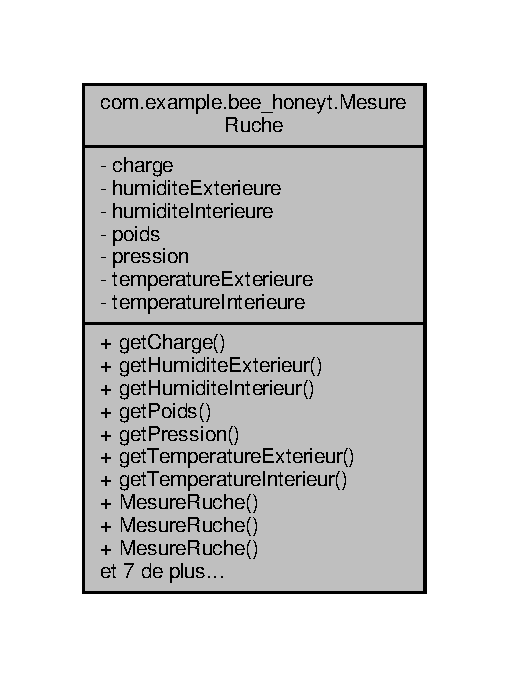
\includegraphics[width=244pt]{classcom_1_1example_1_1bee__honeyt_1_1_mesure_ruche__coll__graph}
\end{center}
\end{figure}
\subsubsection*{Fonctions membres publiques}
\begin{DoxyCompactItemize}
\item 
final int \hyperlink{classcom_1_1example_1_1bee__honeyt_1_1_mesure_ruche_a5fb489924272149140eb7a4c81cacaec}{get\+Charge} ()
\item 
final int \hyperlink{classcom_1_1example_1_1bee__honeyt_1_1_mesure_ruche_ab16738883de0f1535d25bc36b828cc7a}{get\+Humidite\+Exterieur} ()
\item 
final int \hyperlink{classcom_1_1example_1_1bee__honeyt_1_1_mesure_ruche_af78ac1f237287bff4e1a36bebf8bbeef}{get\+Humidite\+Interieur} ()
\item 
final double \hyperlink{classcom_1_1example_1_1bee__honeyt_1_1_mesure_ruche_aff130b4038e223f3ec83769fc354a007}{get\+Poids} ()
\item 
final int \hyperlink{classcom_1_1example_1_1bee__honeyt_1_1_mesure_ruche_a68c21cc141b1103fb3746075657bd4fd}{get\+Pression} ()
\item 
final double \hyperlink{classcom_1_1example_1_1bee__honeyt_1_1_mesure_ruche_a8628b499066f185d78ae015ce50557a8}{get\+Temperature\+Exterieur} ()
\item 
final double \hyperlink{classcom_1_1example_1_1bee__honeyt_1_1_mesure_ruche_ab552e0788fc7dba1e9ef83a0fce861f8}{get\+Temperature\+Interieur} ()
\item 
\hyperlink{classcom_1_1example_1_1bee__honeyt_1_1_mesure_ruche_a3be117936bbcf591ae1a48b6c391f069}{Mesure\+Ruche} ()
\item 
\hyperlink{classcom_1_1example_1_1bee__honeyt_1_1_mesure_ruche_ab9e1fdc4825a5fda8172e6973ce7ec31}{Mesure\+Ruche} (double \hyperlink{classcom_1_1example_1_1bee__honeyt_1_1_mesure_ruche_afd0ecabb4e519d5bcfee33ac15b8b742}{temperature\+Interieure}, double \hyperlink{classcom_1_1example_1_1bee__honeyt_1_1_mesure_ruche_ac13ff0ed6c96cf755097510acf202521}{temperature\+Exterieure}, int \hyperlink{classcom_1_1example_1_1bee__honeyt_1_1_mesure_ruche_a3b5d2536649e0acaf1eebeba4409c9bb}{humidite\+Interieure}, int \hyperlink{classcom_1_1example_1_1bee__honeyt_1_1_mesure_ruche_aa5521e97dfa98051bff9fd8d3ca3f34d}{humidite\+Exterieure}, int \hyperlink{classcom_1_1example_1_1bee__honeyt_1_1_mesure_ruche_ae78080a6d5745faa411e3cfbdbf8aeec}{pression}, double \hyperlink{classcom_1_1example_1_1bee__honeyt_1_1_mesure_ruche_a9aa6c575b7b69c4fb3825944e1f50722}{poids}, int \hyperlink{classcom_1_1example_1_1bee__honeyt_1_1_mesure_ruche_a5ac02bc1d6195faa400e5a3171eed3f4}{charge})
\item 
\hyperlink{classcom_1_1example_1_1bee__honeyt_1_1_mesure_ruche_a1585041919b80789002c833778231a41}{Mesure\+Ruche} (\hyperlink{classcom_1_1example_1_1bee__honeyt_1_1_mesure_ruche}{Mesure\+Ruche} m\+Ruche)
\item 
void \hyperlink{classcom_1_1example_1_1bee__honeyt_1_1_mesure_ruche_aaa185bf82c41c889d3e60804da25bd30}{set\+Charge} (int \hyperlink{classcom_1_1example_1_1bee__honeyt_1_1_mesure_ruche_a5ac02bc1d6195faa400e5a3171eed3f4}{charge})
\item 
void \hyperlink{classcom_1_1example_1_1bee__honeyt_1_1_mesure_ruche_aacb223667567aa9c8a73535f43cda985}{set\+Humidite\+Exterieure} (int \hyperlink{classcom_1_1example_1_1bee__honeyt_1_1_mesure_ruche_aa5521e97dfa98051bff9fd8d3ca3f34d}{humidite\+Exterieure})
\item 
void \hyperlink{classcom_1_1example_1_1bee__honeyt_1_1_mesure_ruche_a8f2d166ffd8340562d9e5cbe5ea5f907}{set\+Humidite\+Interieure} (int \hyperlink{classcom_1_1example_1_1bee__honeyt_1_1_mesure_ruche_a3b5d2536649e0acaf1eebeba4409c9bb}{humidite\+Interieure})
\item 
void \hyperlink{classcom_1_1example_1_1bee__honeyt_1_1_mesure_ruche_aecea2cf7cc504caa34bef93a0e1f3826}{set\+Poids} (double \hyperlink{classcom_1_1example_1_1bee__honeyt_1_1_mesure_ruche_a9aa6c575b7b69c4fb3825944e1f50722}{poids})
\item 
void \hyperlink{classcom_1_1example_1_1bee__honeyt_1_1_mesure_ruche_a87cff86af4a7e977aac1caeaf6a37bc8}{set\+Pression} (int \hyperlink{classcom_1_1example_1_1bee__honeyt_1_1_mesure_ruche_ae78080a6d5745faa411e3cfbdbf8aeec}{pression})
\item 
void \hyperlink{classcom_1_1example_1_1bee__honeyt_1_1_mesure_ruche_a41591480ad8be13a1c7e2e7049dc7935}{set\+Temperature\+Exterieure} (double \hyperlink{classcom_1_1example_1_1bee__honeyt_1_1_mesure_ruche_ac13ff0ed6c96cf755097510acf202521}{temperature\+Exterieure})
\item 
void \hyperlink{classcom_1_1example_1_1bee__honeyt_1_1_mesure_ruche_a5364a38970b37df66bb8cb6f5b3d3741}{set\+Temperature\+Interieure} (double \hyperlink{classcom_1_1example_1_1bee__honeyt_1_1_mesure_ruche_afd0ecabb4e519d5bcfee33ac15b8b742}{temperature\+Interieure})
\end{DoxyCompactItemize}
\subsubsection*{Attributs privés}
\begin{DoxyCompactItemize}
\item 
int \hyperlink{classcom_1_1example_1_1bee__honeyt_1_1_mesure_ruche_a5ac02bc1d6195faa400e5a3171eed3f4}{charge} = 0
\item 
int \hyperlink{classcom_1_1example_1_1bee__honeyt_1_1_mesure_ruche_aa5521e97dfa98051bff9fd8d3ca3f34d}{humidite\+Exterieure} = 0
\item 
int \hyperlink{classcom_1_1example_1_1bee__honeyt_1_1_mesure_ruche_a3b5d2536649e0acaf1eebeba4409c9bb}{humidite\+Interieure} = 0
\item 
double \hyperlink{classcom_1_1example_1_1bee__honeyt_1_1_mesure_ruche_a9aa6c575b7b69c4fb3825944e1f50722}{poids} = 0.\+0
\item 
int \hyperlink{classcom_1_1example_1_1bee__honeyt_1_1_mesure_ruche_ae78080a6d5745faa411e3cfbdbf8aeec}{pression} = 0
\item 
double \hyperlink{classcom_1_1example_1_1bee__honeyt_1_1_mesure_ruche_ac13ff0ed6c96cf755097510acf202521}{temperature\+Exterieure} = 0.\+0
\item 
double \hyperlink{classcom_1_1example_1_1bee__honeyt_1_1_mesure_ruche_afd0ecabb4e519d5bcfee33ac15b8b742}{temperature\+Interieure} = 0.\+0
\end{DoxyCompactItemize}


\subsubsection{Description détaillée}
Les mesures associées à une ruche. 

Définition à la ligne \hyperlink{_mesure_ruche_8java_source_l00015}{15} du fichier \hyperlink{_mesure_ruche_8java_source}{Mesure\+Ruche.\+java}.



\subsubsection{Documentation des constructeurs et destructeur}
\mbox{\Hypertarget{classcom_1_1example_1_1bee__honeyt_1_1_mesure_ruche_a3be117936bbcf591ae1a48b6c391f069}\label{classcom_1_1example_1_1bee__honeyt_1_1_mesure_ruche_a3be117936bbcf591ae1a48b6c391f069}} 
\index{com\+::example\+::bee\+\_\+honeyt\+::\+Mesure\+Ruche@{com\+::example\+::bee\+\_\+honeyt\+::\+Mesure\+Ruche}!Mesure\+Ruche@{Mesure\+Ruche}}
\index{Mesure\+Ruche@{Mesure\+Ruche}!com\+::example\+::bee\+\_\+honeyt\+::\+Mesure\+Ruche@{com\+::example\+::bee\+\_\+honeyt\+::\+Mesure\+Ruche}}
\paragraph{\texorpdfstring{Mesure\+Ruche()}{MesureRuche()}\hspace{0.1cm}{\footnotesize\ttfamily [1/3]}}
{\footnotesize\ttfamily com.\+example.\+bee\+\_\+honeyt.\+Mesure\+Ruche.\+Mesure\+Ruche (\begin{DoxyParamCaption}{ }\end{DoxyParamCaption})}



Définition à la ligne \hyperlink{_mesure_ruche_8java_source_l00025}{25} du fichier \hyperlink{_mesure_ruche_8java_source}{Mesure\+Ruche.\+java}.


\begin{DoxyCode}
00026     \{
00027 
00028     \}
\end{DoxyCode}
\mbox{\Hypertarget{classcom_1_1example_1_1bee__honeyt_1_1_mesure_ruche_ab9e1fdc4825a5fda8172e6973ce7ec31}\label{classcom_1_1example_1_1bee__honeyt_1_1_mesure_ruche_ab9e1fdc4825a5fda8172e6973ce7ec31}} 
\index{com\+::example\+::bee\+\_\+honeyt\+::\+Mesure\+Ruche@{com\+::example\+::bee\+\_\+honeyt\+::\+Mesure\+Ruche}!Mesure\+Ruche@{Mesure\+Ruche}}
\index{Mesure\+Ruche@{Mesure\+Ruche}!com\+::example\+::bee\+\_\+honeyt\+::\+Mesure\+Ruche@{com\+::example\+::bee\+\_\+honeyt\+::\+Mesure\+Ruche}}
\paragraph{\texorpdfstring{Mesure\+Ruche()}{MesureRuche()}\hspace{0.1cm}{\footnotesize\ttfamily [2/3]}}
{\footnotesize\ttfamily com.\+example.\+bee\+\_\+honeyt.\+Mesure\+Ruche.\+Mesure\+Ruche (\begin{DoxyParamCaption}\item[{double}]{temperature\+Interieure,  }\item[{double}]{temperature\+Exterieure,  }\item[{int}]{humidite\+Interieure,  }\item[{int}]{humidite\+Exterieure,  }\item[{int}]{pression,  }\item[{double}]{poids,  }\item[{int}]{charge }\end{DoxyParamCaption})}



Définition à la ligne \hyperlink{_mesure_ruche_8java_source_l00030}{30} du fichier \hyperlink{_mesure_ruche_8java_source}{Mesure\+Ruche.\+java}.



Références \hyperlink{_mesure_ruche_8java_source_l00023}{com.\+example.\+bee\+\_\+honeyt.\+Mesure\+Ruche.\+charge}, \hyperlink{_mesure_ruche_8java_source_l00020}{com.\+example.\+bee\+\_\+honeyt.\+Mesure\+Ruche.\+humidite\+Exterieure}, \hyperlink{_mesure_ruche_8java_source_l00019}{com.\+example.\+bee\+\_\+honeyt.\+Mesure\+Ruche.\+humidite\+Interieure}, \hyperlink{_mesure_ruche_8java_source_l00022}{com.\+example.\+bee\+\_\+honeyt.\+Mesure\+Ruche.\+poids}, \hyperlink{_mesure_ruche_8java_source_l00021}{com.\+example.\+bee\+\_\+honeyt.\+Mesure\+Ruche.\+pression}, \hyperlink{_mesure_ruche_8java_source_l00018}{com.\+example.\+bee\+\_\+honeyt.\+Mesure\+Ruche.\+temperature\+Exterieure}, et \hyperlink{_mesure_ruche_8java_source_l00017}{com.\+example.\+bee\+\_\+honeyt.\+Mesure\+Ruche.\+temperature\+Interieure}.


\begin{DoxyCode}
00031     \{
00032         this.\hyperlink{classcom_1_1example_1_1bee__honeyt_1_1_mesure_ruche_afd0ecabb4e519d5bcfee33ac15b8b742}{temperatureInterieure} = \hyperlink{classcom_1_1example_1_1bee__honeyt_1_1_mesure_ruche_afd0ecabb4e519d5bcfee33ac15b8b742}{temperatureInterieure};
00033         this.\hyperlink{classcom_1_1example_1_1bee__honeyt_1_1_mesure_ruche_ac13ff0ed6c96cf755097510acf202521}{temperatureExterieure} = \hyperlink{classcom_1_1example_1_1bee__honeyt_1_1_mesure_ruche_ac13ff0ed6c96cf755097510acf202521}{temperatureExterieure};
00034         this.\hyperlink{classcom_1_1example_1_1bee__honeyt_1_1_mesure_ruche_a3b5d2536649e0acaf1eebeba4409c9bb}{humiditeInterieure} = \hyperlink{classcom_1_1example_1_1bee__honeyt_1_1_mesure_ruche_a3b5d2536649e0acaf1eebeba4409c9bb}{humiditeInterieure};
00035         this.\hyperlink{classcom_1_1example_1_1bee__honeyt_1_1_mesure_ruche_aa5521e97dfa98051bff9fd8d3ca3f34d}{humiditeExterieure} = \hyperlink{classcom_1_1example_1_1bee__honeyt_1_1_mesure_ruche_aa5521e97dfa98051bff9fd8d3ca3f34d}{humiditeExterieure};
00036         this.\hyperlink{classcom_1_1example_1_1bee__honeyt_1_1_mesure_ruche_ae78080a6d5745faa411e3cfbdbf8aeec}{pression} = \hyperlink{classcom_1_1example_1_1bee__honeyt_1_1_mesure_ruche_ae78080a6d5745faa411e3cfbdbf8aeec}{pression};
00037         this.\hyperlink{classcom_1_1example_1_1bee__honeyt_1_1_mesure_ruche_a9aa6c575b7b69c4fb3825944e1f50722}{poids} = \hyperlink{classcom_1_1example_1_1bee__honeyt_1_1_mesure_ruche_a9aa6c575b7b69c4fb3825944e1f50722}{poids};
00038         this.\hyperlink{classcom_1_1example_1_1bee__honeyt_1_1_mesure_ruche_a5ac02bc1d6195faa400e5a3171eed3f4}{charge} = \hyperlink{classcom_1_1example_1_1bee__honeyt_1_1_mesure_ruche_a5ac02bc1d6195faa400e5a3171eed3f4}{charge};
00039     \}
\end{DoxyCode}
\mbox{\Hypertarget{classcom_1_1example_1_1bee__honeyt_1_1_mesure_ruche_a1585041919b80789002c833778231a41}\label{classcom_1_1example_1_1bee__honeyt_1_1_mesure_ruche_a1585041919b80789002c833778231a41}} 
\index{com\+::example\+::bee\+\_\+honeyt\+::\+Mesure\+Ruche@{com\+::example\+::bee\+\_\+honeyt\+::\+Mesure\+Ruche}!Mesure\+Ruche@{Mesure\+Ruche}}
\index{Mesure\+Ruche@{Mesure\+Ruche}!com\+::example\+::bee\+\_\+honeyt\+::\+Mesure\+Ruche@{com\+::example\+::bee\+\_\+honeyt\+::\+Mesure\+Ruche}}
\paragraph{\texorpdfstring{Mesure\+Ruche()}{MesureRuche()}\hspace{0.1cm}{\footnotesize\ttfamily [3/3]}}
{\footnotesize\ttfamily com.\+example.\+bee\+\_\+honeyt.\+Mesure\+Ruche.\+Mesure\+Ruche (\begin{DoxyParamCaption}\item[{\hyperlink{classcom_1_1example_1_1bee__honeyt_1_1_mesure_ruche}{Mesure\+Ruche}}]{m\+Ruche }\end{DoxyParamCaption})}



Définition à la ligne \hyperlink{_mesure_ruche_8java_source_l00041}{41} du fichier \hyperlink{_mesure_ruche_8java_source}{Mesure\+Ruche.\+java}.



Références \hyperlink{_mesure_ruche_8java_source_l00023}{com.\+example.\+bee\+\_\+honeyt.\+Mesure\+Ruche.\+charge}, \hyperlink{_mesure_ruche_8java_source_l00020}{com.\+example.\+bee\+\_\+honeyt.\+Mesure\+Ruche.\+humidite\+Exterieure}, \hyperlink{_mesure_ruche_8java_source_l00019}{com.\+example.\+bee\+\_\+honeyt.\+Mesure\+Ruche.\+humidite\+Interieure}, \hyperlink{_mesure_ruche_8java_source_l00022}{com.\+example.\+bee\+\_\+honeyt.\+Mesure\+Ruche.\+poids}, \hyperlink{_mesure_ruche_8java_source_l00021}{com.\+example.\+bee\+\_\+honeyt.\+Mesure\+Ruche.\+pression}, \hyperlink{_mesure_ruche_8java_source_l00018}{com.\+example.\+bee\+\_\+honeyt.\+Mesure\+Ruche.\+temperature\+Exterieure}, et \hyperlink{_mesure_ruche_8java_source_l00017}{com.\+example.\+bee\+\_\+honeyt.\+Mesure\+Ruche.\+temperature\+Interieure}.


\begin{DoxyCode}
00042     \{
00043         this.\hyperlink{classcom_1_1example_1_1bee__honeyt_1_1_mesure_ruche_afd0ecabb4e519d5bcfee33ac15b8b742}{temperatureInterieure} = mRuche.temperatureInterieure;
00044         this.\hyperlink{classcom_1_1example_1_1bee__honeyt_1_1_mesure_ruche_ac13ff0ed6c96cf755097510acf202521}{temperatureExterieure} = mRuche.temperatureExterieure;
00045         this.\hyperlink{classcom_1_1example_1_1bee__honeyt_1_1_mesure_ruche_a3b5d2536649e0acaf1eebeba4409c9bb}{humiditeInterieure} = mRuche.humiditeInterieure;
00046         this.\hyperlink{classcom_1_1example_1_1bee__honeyt_1_1_mesure_ruche_aa5521e97dfa98051bff9fd8d3ca3f34d}{humiditeExterieure} = mRuche.humiditeExterieure;
00047         this.\hyperlink{classcom_1_1example_1_1bee__honeyt_1_1_mesure_ruche_ae78080a6d5745faa411e3cfbdbf8aeec}{pression} = mRuche.pression;
00048         this.\hyperlink{classcom_1_1example_1_1bee__honeyt_1_1_mesure_ruche_a9aa6c575b7b69c4fb3825944e1f50722}{poids} = mRuche.poids;
00049         this.\hyperlink{classcom_1_1example_1_1bee__honeyt_1_1_mesure_ruche_a5ac02bc1d6195faa400e5a3171eed3f4}{charge} = mRuche.charge;
00050     \}
\end{DoxyCode}


\subsubsection{Documentation des fonctions membres}
\mbox{\Hypertarget{classcom_1_1example_1_1bee__honeyt_1_1_mesure_ruche_a5fb489924272149140eb7a4c81cacaec}\label{classcom_1_1example_1_1bee__honeyt_1_1_mesure_ruche_a5fb489924272149140eb7a4c81cacaec}} 
\index{com\+::example\+::bee\+\_\+honeyt\+::\+Mesure\+Ruche@{com\+::example\+::bee\+\_\+honeyt\+::\+Mesure\+Ruche}!get\+Charge@{get\+Charge}}
\index{get\+Charge@{get\+Charge}!com\+::example\+::bee\+\_\+honeyt\+::\+Mesure\+Ruche@{com\+::example\+::bee\+\_\+honeyt\+::\+Mesure\+Ruche}}
\paragraph{\texorpdfstring{get\+Charge()}{getCharge()}}
{\footnotesize\ttfamily final int com.\+example.\+bee\+\_\+honeyt.\+Mesure\+Ruche.\+get\+Charge (\begin{DoxyParamCaption}{ }\end{DoxyParamCaption})}



Définition à la ligne \hyperlink{_mesure_ruche_8java_source_l00112}{112} du fichier \hyperlink{_mesure_ruche_8java_source}{Mesure\+Ruche.\+java}.



Références \hyperlink{_mesure_ruche_8java_source_l00023}{com.\+example.\+bee\+\_\+honeyt.\+Mesure\+Ruche.\+charge}.



Référencé par \hyperlink{_i_h_m_mobile_8java_source_l00170}{com.\+example.\+bee\+\_\+honeyt.\+I\+H\+M\+Mobile.\+initialiser\+Liste\+Ruches()}.


\begin{DoxyCode}
00112 \{ \textcolor{keywordflow}{return} \hyperlink{classcom_1_1example_1_1bee__honeyt_1_1_mesure_ruche_a5ac02bc1d6195faa400e5a3171eed3f4}{charge}; \}
\end{DoxyCode}
\mbox{\Hypertarget{classcom_1_1example_1_1bee__honeyt_1_1_mesure_ruche_ab16738883de0f1535d25bc36b828cc7a}\label{classcom_1_1example_1_1bee__honeyt_1_1_mesure_ruche_ab16738883de0f1535d25bc36b828cc7a}} 
\index{com\+::example\+::bee\+\_\+honeyt\+::\+Mesure\+Ruche@{com\+::example\+::bee\+\_\+honeyt\+::\+Mesure\+Ruche}!get\+Humidite\+Exterieur@{get\+Humidite\+Exterieur}}
\index{get\+Humidite\+Exterieur@{get\+Humidite\+Exterieur}!com\+::example\+::bee\+\_\+honeyt\+::\+Mesure\+Ruche@{com\+::example\+::bee\+\_\+honeyt\+::\+Mesure\+Ruche}}
\paragraph{\texorpdfstring{get\+Humidite\+Exterieur()}{getHumiditeExterieur()}}
{\footnotesize\ttfamily final int com.\+example.\+bee\+\_\+honeyt.\+Mesure\+Ruche.\+get\+Humidite\+Exterieur (\begin{DoxyParamCaption}{ }\end{DoxyParamCaption})}



Définition à la ligne \hyperlink{_mesure_ruche_8java_source_l00082}{82} du fichier \hyperlink{_mesure_ruche_8java_source}{Mesure\+Ruche.\+java}.



Références \hyperlink{_mesure_ruche_8java_source_l00020}{com.\+example.\+bee\+\_\+honeyt.\+Mesure\+Ruche.\+humidite\+Exterieure}.



Référencé par \hyperlink{_i_h_m_mobile_8java_source_l00170}{com.\+example.\+bee\+\_\+honeyt.\+I\+H\+M\+Mobile.\+initialiser\+Liste\+Ruches()}.


\begin{DoxyCode}
00083     \{
00084         \textcolor{keywordflow}{return} \hyperlink{classcom_1_1example_1_1bee__honeyt_1_1_mesure_ruche_aa5521e97dfa98051bff9fd8d3ca3f34d}{humiditeExterieure};
00085     \}
\end{DoxyCode}
\mbox{\Hypertarget{classcom_1_1example_1_1bee__honeyt_1_1_mesure_ruche_af78ac1f237287bff4e1a36bebf8bbeef}\label{classcom_1_1example_1_1bee__honeyt_1_1_mesure_ruche_af78ac1f237287bff4e1a36bebf8bbeef}} 
\index{com\+::example\+::bee\+\_\+honeyt\+::\+Mesure\+Ruche@{com\+::example\+::bee\+\_\+honeyt\+::\+Mesure\+Ruche}!get\+Humidite\+Interieur@{get\+Humidite\+Interieur}}
\index{get\+Humidite\+Interieur@{get\+Humidite\+Interieur}!com\+::example\+::bee\+\_\+honeyt\+::\+Mesure\+Ruche@{com\+::example\+::bee\+\_\+honeyt\+::\+Mesure\+Ruche}}
\paragraph{\texorpdfstring{get\+Humidite\+Interieur()}{getHumiditeInterieur()}}
{\footnotesize\ttfamily final int com.\+example.\+bee\+\_\+honeyt.\+Mesure\+Ruche.\+get\+Humidite\+Interieur (\begin{DoxyParamCaption}{ }\end{DoxyParamCaption})}



Définition à la ligne \hyperlink{_mesure_ruche_8java_source_l00072}{72} du fichier \hyperlink{_mesure_ruche_8java_source}{Mesure\+Ruche.\+java}.



Références \hyperlink{_mesure_ruche_8java_source_l00019}{com.\+example.\+bee\+\_\+honeyt.\+Mesure\+Ruche.\+humidite\+Interieure}.



Référencé par \hyperlink{_i_h_m_mobile_8java_source_l00170}{com.\+example.\+bee\+\_\+honeyt.\+I\+H\+M\+Mobile.\+initialiser\+Liste\+Ruches()}.


\begin{DoxyCode}
00073     \{
00074         \textcolor{keywordflow}{return} \hyperlink{classcom_1_1example_1_1bee__honeyt_1_1_mesure_ruche_a3b5d2536649e0acaf1eebeba4409c9bb}{humiditeInterieure};
00075     \}
\end{DoxyCode}
\mbox{\Hypertarget{classcom_1_1example_1_1bee__honeyt_1_1_mesure_ruche_aff130b4038e223f3ec83769fc354a007}\label{classcom_1_1example_1_1bee__honeyt_1_1_mesure_ruche_aff130b4038e223f3ec83769fc354a007}} 
\index{com\+::example\+::bee\+\_\+honeyt\+::\+Mesure\+Ruche@{com\+::example\+::bee\+\_\+honeyt\+::\+Mesure\+Ruche}!get\+Poids@{get\+Poids}}
\index{get\+Poids@{get\+Poids}!com\+::example\+::bee\+\_\+honeyt\+::\+Mesure\+Ruche@{com\+::example\+::bee\+\_\+honeyt\+::\+Mesure\+Ruche}}
\paragraph{\texorpdfstring{get\+Poids()}{getPoids()}}
{\footnotesize\ttfamily final double com.\+example.\+bee\+\_\+honeyt.\+Mesure\+Ruche.\+get\+Poids (\begin{DoxyParamCaption}{ }\end{DoxyParamCaption})}



Définition à la ligne \hyperlink{_mesure_ruche_8java_source_l00102}{102} du fichier \hyperlink{_mesure_ruche_8java_source}{Mesure\+Ruche.\+java}.



Références \hyperlink{_mesure_ruche_8java_source_l00022}{com.\+example.\+bee\+\_\+honeyt.\+Mesure\+Ruche.\+poids}.



Référencé par \hyperlink{_i_h_m_mobile_8java_source_l00170}{com.\+example.\+bee\+\_\+honeyt.\+I\+H\+M\+Mobile.\+initialiser\+Liste\+Ruches()}.


\begin{DoxyCode}
00103     \{
00104         \textcolor{keywordflow}{return} \hyperlink{classcom_1_1example_1_1bee__honeyt_1_1_mesure_ruche_a9aa6c575b7b69c4fb3825944e1f50722}{poids};
00105     \}
\end{DoxyCode}
\mbox{\Hypertarget{classcom_1_1example_1_1bee__honeyt_1_1_mesure_ruche_a68c21cc141b1103fb3746075657bd4fd}\label{classcom_1_1example_1_1bee__honeyt_1_1_mesure_ruche_a68c21cc141b1103fb3746075657bd4fd}} 
\index{com\+::example\+::bee\+\_\+honeyt\+::\+Mesure\+Ruche@{com\+::example\+::bee\+\_\+honeyt\+::\+Mesure\+Ruche}!get\+Pression@{get\+Pression}}
\index{get\+Pression@{get\+Pression}!com\+::example\+::bee\+\_\+honeyt\+::\+Mesure\+Ruche@{com\+::example\+::bee\+\_\+honeyt\+::\+Mesure\+Ruche}}
\paragraph{\texorpdfstring{get\+Pression()}{getPression()}}
{\footnotesize\ttfamily final int com.\+example.\+bee\+\_\+honeyt.\+Mesure\+Ruche.\+get\+Pression (\begin{DoxyParamCaption}{ }\end{DoxyParamCaption})}



Définition à la ligne \hyperlink{_mesure_ruche_8java_source_l00092}{92} du fichier \hyperlink{_mesure_ruche_8java_source}{Mesure\+Ruche.\+java}.



Références \hyperlink{_mesure_ruche_8java_source_l00021}{com.\+example.\+bee\+\_\+honeyt.\+Mesure\+Ruche.\+pression}.



Référencé par \hyperlink{_i_h_m_mobile_8java_source_l00170}{com.\+example.\+bee\+\_\+honeyt.\+I\+H\+M\+Mobile.\+initialiser\+Liste\+Ruches()}.


\begin{DoxyCode}
00093     \{
00094         \textcolor{keywordflow}{return} \hyperlink{classcom_1_1example_1_1bee__honeyt_1_1_mesure_ruche_ae78080a6d5745faa411e3cfbdbf8aeec}{pression};
00095     \}
\end{DoxyCode}
\mbox{\Hypertarget{classcom_1_1example_1_1bee__honeyt_1_1_mesure_ruche_a8628b499066f185d78ae015ce50557a8}\label{classcom_1_1example_1_1bee__honeyt_1_1_mesure_ruche_a8628b499066f185d78ae015ce50557a8}} 
\index{com\+::example\+::bee\+\_\+honeyt\+::\+Mesure\+Ruche@{com\+::example\+::bee\+\_\+honeyt\+::\+Mesure\+Ruche}!get\+Temperature\+Exterieur@{get\+Temperature\+Exterieur}}
\index{get\+Temperature\+Exterieur@{get\+Temperature\+Exterieur}!com\+::example\+::bee\+\_\+honeyt\+::\+Mesure\+Ruche@{com\+::example\+::bee\+\_\+honeyt\+::\+Mesure\+Ruche}}
\paragraph{\texorpdfstring{get\+Temperature\+Exterieur()}{getTemperatureExterieur()}}
{\footnotesize\ttfamily final double com.\+example.\+bee\+\_\+honeyt.\+Mesure\+Ruche.\+get\+Temperature\+Exterieur (\begin{DoxyParamCaption}{ }\end{DoxyParamCaption})}



Définition à la ligne \hyperlink{_mesure_ruche_8java_source_l00062}{62} du fichier \hyperlink{_mesure_ruche_8java_source}{Mesure\+Ruche.\+java}.



Références \hyperlink{_mesure_ruche_8java_source_l00018}{com.\+example.\+bee\+\_\+honeyt.\+Mesure\+Ruche.\+temperature\+Exterieure}.



Référencé par \hyperlink{_i_h_m_mobile_8java_source_l00170}{com.\+example.\+bee\+\_\+honeyt.\+I\+H\+M\+Mobile.\+initialiser\+Liste\+Ruches()}.


\begin{DoxyCode}
00063     \{
00064         \textcolor{keywordflow}{return} \hyperlink{classcom_1_1example_1_1bee__honeyt_1_1_mesure_ruche_ac13ff0ed6c96cf755097510acf202521}{temperatureExterieure};
00065     \}
\end{DoxyCode}
\mbox{\Hypertarget{classcom_1_1example_1_1bee__honeyt_1_1_mesure_ruche_ab552e0788fc7dba1e9ef83a0fce861f8}\label{classcom_1_1example_1_1bee__honeyt_1_1_mesure_ruche_ab552e0788fc7dba1e9ef83a0fce861f8}} 
\index{com\+::example\+::bee\+\_\+honeyt\+::\+Mesure\+Ruche@{com\+::example\+::bee\+\_\+honeyt\+::\+Mesure\+Ruche}!get\+Temperature\+Interieur@{get\+Temperature\+Interieur}}
\index{get\+Temperature\+Interieur@{get\+Temperature\+Interieur}!com\+::example\+::bee\+\_\+honeyt\+::\+Mesure\+Ruche@{com\+::example\+::bee\+\_\+honeyt\+::\+Mesure\+Ruche}}
\paragraph{\texorpdfstring{get\+Temperature\+Interieur()}{getTemperatureInterieur()}}
{\footnotesize\ttfamily final double com.\+example.\+bee\+\_\+honeyt.\+Mesure\+Ruche.\+get\+Temperature\+Interieur (\begin{DoxyParamCaption}{ }\end{DoxyParamCaption})}



Définition à la ligne \hyperlink{_mesure_ruche_8java_source_l00052}{52} du fichier \hyperlink{_mesure_ruche_8java_source}{Mesure\+Ruche.\+java}.



Références \hyperlink{_mesure_ruche_8java_source_l00017}{com.\+example.\+bee\+\_\+honeyt.\+Mesure\+Ruche.\+temperature\+Interieure}.



Référencé par \hyperlink{_i_h_m_mobile_8java_source_l00170}{com.\+example.\+bee\+\_\+honeyt.\+I\+H\+M\+Mobile.\+initialiser\+Liste\+Ruches()}.


\begin{DoxyCode}
00053     \{
00054         \textcolor{keywordflow}{return} \hyperlink{classcom_1_1example_1_1bee__honeyt_1_1_mesure_ruche_afd0ecabb4e519d5bcfee33ac15b8b742}{temperatureInterieure};
00055     \}
\end{DoxyCode}
\mbox{\Hypertarget{classcom_1_1example_1_1bee__honeyt_1_1_mesure_ruche_aaa185bf82c41c889d3e60804da25bd30}\label{classcom_1_1example_1_1bee__honeyt_1_1_mesure_ruche_aaa185bf82c41c889d3e60804da25bd30}} 
\index{com\+::example\+::bee\+\_\+honeyt\+::\+Mesure\+Ruche@{com\+::example\+::bee\+\_\+honeyt\+::\+Mesure\+Ruche}!set\+Charge@{set\+Charge}}
\index{set\+Charge@{set\+Charge}!com\+::example\+::bee\+\_\+honeyt\+::\+Mesure\+Ruche@{com\+::example\+::bee\+\_\+honeyt\+::\+Mesure\+Ruche}}
\paragraph{\texorpdfstring{set\+Charge()}{setCharge()}}
{\footnotesize\ttfamily void com.\+example.\+bee\+\_\+honeyt.\+Mesure\+Ruche.\+set\+Charge (\begin{DoxyParamCaption}\item[{int}]{charge }\end{DoxyParamCaption})}



Définition à la ligne \hyperlink{_mesure_ruche_8java_source_l00114}{114} du fichier \hyperlink{_mesure_ruche_8java_source}{Mesure\+Ruche.\+java}.



Références \hyperlink{_mesure_ruche_8java_source_l00023}{com.\+example.\+bee\+\_\+honeyt.\+Mesure\+Ruche.\+charge}.



Référencé par \hyperlink{_i_h_m_mobile_8java_source_l00374}{com.\+example.\+bee\+\_\+honeyt.\+I\+H\+M\+Mobile.\+traiter\+Message()}.


\begin{DoxyCode}
00115     \{
00116         this.\hyperlink{classcom_1_1example_1_1bee__honeyt_1_1_mesure_ruche_a5ac02bc1d6195faa400e5a3171eed3f4}{charge} = \hyperlink{classcom_1_1example_1_1bee__honeyt_1_1_mesure_ruche_a5ac02bc1d6195faa400e5a3171eed3f4}{charge};
00117     \}
\end{DoxyCode}
\mbox{\Hypertarget{classcom_1_1example_1_1bee__honeyt_1_1_mesure_ruche_aacb223667567aa9c8a73535f43cda985}\label{classcom_1_1example_1_1bee__honeyt_1_1_mesure_ruche_aacb223667567aa9c8a73535f43cda985}} 
\index{com\+::example\+::bee\+\_\+honeyt\+::\+Mesure\+Ruche@{com\+::example\+::bee\+\_\+honeyt\+::\+Mesure\+Ruche}!set\+Humidite\+Exterieure@{set\+Humidite\+Exterieure}}
\index{set\+Humidite\+Exterieure@{set\+Humidite\+Exterieure}!com\+::example\+::bee\+\_\+honeyt\+::\+Mesure\+Ruche@{com\+::example\+::bee\+\_\+honeyt\+::\+Mesure\+Ruche}}
\paragraph{\texorpdfstring{set\+Humidite\+Exterieure()}{setHumiditeExterieure()}}
{\footnotesize\ttfamily void com.\+example.\+bee\+\_\+honeyt.\+Mesure\+Ruche.\+set\+Humidite\+Exterieure (\begin{DoxyParamCaption}\item[{int}]{humidite\+Exterieure }\end{DoxyParamCaption})}



Définition à la ligne \hyperlink{_mesure_ruche_8java_source_l00087}{87} du fichier \hyperlink{_mesure_ruche_8java_source}{Mesure\+Ruche.\+java}.



Références \hyperlink{_mesure_ruche_8java_source_l00020}{com.\+example.\+bee\+\_\+honeyt.\+Mesure\+Ruche.\+humidite\+Exterieure}.



Référencé par \hyperlink{_i_h_m_mobile_8java_source_l00374}{com.\+example.\+bee\+\_\+honeyt.\+I\+H\+M\+Mobile.\+traiter\+Message()}.


\begin{DoxyCode}
00088     \{
00089         this.\hyperlink{classcom_1_1example_1_1bee__honeyt_1_1_mesure_ruche_aa5521e97dfa98051bff9fd8d3ca3f34d}{humiditeExterieure} = \hyperlink{classcom_1_1example_1_1bee__honeyt_1_1_mesure_ruche_aa5521e97dfa98051bff9fd8d3ca3f34d}{humiditeExterieure};
00090     \}
\end{DoxyCode}
\mbox{\Hypertarget{classcom_1_1example_1_1bee__honeyt_1_1_mesure_ruche_a8f2d166ffd8340562d9e5cbe5ea5f907}\label{classcom_1_1example_1_1bee__honeyt_1_1_mesure_ruche_a8f2d166ffd8340562d9e5cbe5ea5f907}} 
\index{com\+::example\+::bee\+\_\+honeyt\+::\+Mesure\+Ruche@{com\+::example\+::bee\+\_\+honeyt\+::\+Mesure\+Ruche}!set\+Humidite\+Interieure@{set\+Humidite\+Interieure}}
\index{set\+Humidite\+Interieure@{set\+Humidite\+Interieure}!com\+::example\+::bee\+\_\+honeyt\+::\+Mesure\+Ruche@{com\+::example\+::bee\+\_\+honeyt\+::\+Mesure\+Ruche}}
\paragraph{\texorpdfstring{set\+Humidite\+Interieure()}{setHumiditeInterieure()}}
{\footnotesize\ttfamily void com.\+example.\+bee\+\_\+honeyt.\+Mesure\+Ruche.\+set\+Humidite\+Interieure (\begin{DoxyParamCaption}\item[{int}]{humidite\+Interieure }\end{DoxyParamCaption})}



Définition à la ligne \hyperlink{_mesure_ruche_8java_source_l00077}{77} du fichier \hyperlink{_mesure_ruche_8java_source}{Mesure\+Ruche.\+java}.



Références \hyperlink{_mesure_ruche_8java_source_l00019}{com.\+example.\+bee\+\_\+honeyt.\+Mesure\+Ruche.\+humidite\+Interieure}.



Référencé par \hyperlink{_i_h_m_mobile_8java_source_l00374}{com.\+example.\+bee\+\_\+honeyt.\+I\+H\+M\+Mobile.\+traiter\+Message()}.


\begin{DoxyCode}
00078     \{
00079         this.\hyperlink{classcom_1_1example_1_1bee__honeyt_1_1_mesure_ruche_a3b5d2536649e0acaf1eebeba4409c9bb}{humiditeInterieure} = \hyperlink{classcom_1_1example_1_1bee__honeyt_1_1_mesure_ruche_a3b5d2536649e0acaf1eebeba4409c9bb}{humiditeInterieure};
00080     \}
\end{DoxyCode}
\mbox{\Hypertarget{classcom_1_1example_1_1bee__honeyt_1_1_mesure_ruche_aecea2cf7cc504caa34bef93a0e1f3826}\label{classcom_1_1example_1_1bee__honeyt_1_1_mesure_ruche_aecea2cf7cc504caa34bef93a0e1f3826}} 
\index{com\+::example\+::bee\+\_\+honeyt\+::\+Mesure\+Ruche@{com\+::example\+::bee\+\_\+honeyt\+::\+Mesure\+Ruche}!set\+Poids@{set\+Poids}}
\index{set\+Poids@{set\+Poids}!com\+::example\+::bee\+\_\+honeyt\+::\+Mesure\+Ruche@{com\+::example\+::bee\+\_\+honeyt\+::\+Mesure\+Ruche}}
\paragraph{\texorpdfstring{set\+Poids()}{setPoids()}}
{\footnotesize\ttfamily void com.\+example.\+bee\+\_\+honeyt.\+Mesure\+Ruche.\+set\+Poids (\begin{DoxyParamCaption}\item[{double}]{poids }\end{DoxyParamCaption})}



Définition à la ligne \hyperlink{_mesure_ruche_8java_source_l00107}{107} du fichier \hyperlink{_mesure_ruche_8java_source}{Mesure\+Ruche.\+java}.



Références \hyperlink{_mesure_ruche_8java_source_l00022}{com.\+example.\+bee\+\_\+honeyt.\+Mesure\+Ruche.\+poids}.


\begin{DoxyCode}
00108     \{
00109         this.\hyperlink{classcom_1_1example_1_1bee__honeyt_1_1_mesure_ruche_a9aa6c575b7b69c4fb3825944e1f50722}{poids} = \hyperlink{classcom_1_1example_1_1bee__honeyt_1_1_mesure_ruche_a9aa6c575b7b69c4fb3825944e1f50722}{poids};
00110     \}
\end{DoxyCode}
\mbox{\Hypertarget{classcom_1_1example_1_1bee__honeyt_1_1_mesure_ruche_a87cff86af4a7e977aac1caeaf6a37bc8}\label{classcom_1_1example_1_1bee__honeyt_1_1_mesure_ruche_a87cff86af4a7e977aac1caeaf6a37bc8}} 
\index{com\+::example\+::bee\+\_\+honeyt\+::\+Mesure\+Ruche@{com\+::example\+::bee\+\_\+honeyt\+::\+Mesure\+Ruche}!set\+Pression@{set\+Pression}}
\index{set\+Pression@{set\+Pression}!com\+::example\+::bee\+\_\+honeyt\+::\+Mesure\+Ruche@{com\+::example\+::bee\+\_\+honeyt\+::\+Mesure\+Ruche}}
\paragraph{\texorpdfstring{set\+Pression()}{setPression()}}
{\footnotesize\ttfamily void com.\+example.\+bee\+\_\+honeyt.\+Mesure\+Ruche.\+set\+Pression (\begin{DoxyParamCaption}\item[{int}]{pression }\end{DoxyParamCaption})}



Définition à la ligne \hyperlink{_mesure_ruche_8java_source_l00097}{97} du fichier \hyperlink{_mesure_ruche_8java_source}{Mesure\+Ruche.\+java}.



Références \hyperlink{_mesure_ruche_8java_source_l00021}{com.\+example.\+bee\+\_\+honeyt.\+Mesure\+Ruche.\+pression}.



Référencé par \hyperlink{_i_h_m_mobile_8java_source_l00374}{com.\+example.\+bee\+\_\+honeyt.\+I\+H\+M\+Mobile.\+traiter\+Message()}.


\begin{DoxyCode}
00098     \{
00099         this.\hyperlink{classcom_1_1example_1_1bee__honeyt_1_1_mesure_ruche_ae78080a6d5745faa411e3cfbdbf8aeec}{pression} = \hyperlink{classcom_1_1example_1_1bee__honeyt_1_1_mesure_ruche_ae78080a6d5745faa411e3cfbdbf8aeec}{pression};
00100     \}
\end{DoxyCode}
\mbox{\Hypertarget{classcom_1_1example_1_1bee__honeyt_1_1_mesure_ruche_a41591480ad8be13a1c7e2e7049dc7935}\label{classcom_1_1example_1_1bee__honeyt_1_1_mesure_ruche_a41591480ad8be13a1c7e2e7049dc7935}} 
\index{com\+::example\+::bee\+\_\+honeyt\+::\+Mesure\+Ruche@{com\+::example\+::bee\+\_\+honeyt\+::\+Mesure\+Ruche}!set\+Temperature\+Exterieure@{set\+Temperature\+Exterieure}}
\index{set\+Temperature\+Exterieure@{set\+Temperature\+Exterieure}!com\+::example\+::bee\+\_\+honeyt\+::\+Mesure\+Ruche@{com\+::example\+::bee\+\_\+honeyt\+::\+Mesure\+Ruche}}
\paragraph{\texorpdfstring{set\+Temperature\+Exterieure()}{setTemperatureExterieure()}}
{\footnotesize\ttfamily void com.\+example.\+bee\+\_\+honeyt.\+Mesure\+Ruche.\+set\+Temperature\+Exterieure (\begin{DoxyParamCaption}\item[{double}]{temperature\+Exterieure }\end{DoxyParamCaption})}



Définition à la ligne \hyperlink{_mesure_ruche_8java_source_l00067}{67} du fichier \hyperlink{_mesure_ruche_8java_source}{Mesure\+Ruche.\+java}.



Références \hyperlink{_mesure_ruche_8java_source_l00018}{com.\+example.\+bee\+\_\+honeyt.\+Mesure\+Ruche.\+temperature\+Exterieure}.



Référencé par \hyperlink{_i_h_m_mobile_8java_source_l00374}{com.\+example.\+bee\+\_\+honeyt.\+I\+H\+M\+Mobile.\+traiter\+Message()}.


\begin{DoxyCode}
00068     \{
00069         this.\hyperlink{classcom_1_1example_1_1bee__honeyt_1_1_mesure_ruche_ac13ff0ed6c96cf755097510acf202521}{temperatureExterieure} = \hyperlink{classcom_1_1example_1_1bee__honeyt_1_1_mesure_ruche_ac13ff0ed6c96cf755097510acf202521}{temperatureExterieure};
00070     \}
\end{DoxyCode}
\mbox{\Hypertarget{classcom_1_1example_1_1bee__honeyt_1_1_mesure_ruche_a5364a38970b37df66bb8cb6f5b3d3741}\label{classcom_1_1example_1_1bee__honeyt_1_1_mesure_ruche_a5364a38970b37df66bb8cb6f5b3d3741}} 
\index{com\+::example\+::bee\+\_\+honeyt\+::\+Mesure\+Ruche@{com\+::example\+::bee\+\_\+honeyt\+::\+Mesure\+Ruche}!set\+Temperature\+Interieure@{set\+Temperature\+Interieure}}
\index{set\+Temperature\+Interieure@{set\+Temperature\+Interieure}!com\+::example\+::bee\+\_\+honeyt\+::\+Mesure\+Ruche@{com\+::example\+::bee\+\_\+honeyt\+::\+Mesure\+Ruche}}
\paragraph{\texorpdfstring{set\+Temperature\+Interieure()}{setTemperatureInterieure()}}
{\footnotesize\ttfamily void com.\+example.\+bee\+\_\+honeyt.\+Mesure\+Ruche.\+set\+Temperature\+Interieure (\begin{DoxyParamCaption}\item[{double}]{temperature\+Interieure }\end{DoxyParamCaption})}



Définition à la ligne \hyperlink{_mesure_ruche_8java_source_l00057}{57} du fichier \hyperlink{_mesure_ruche_8java_source}{Mesure\+Ruche.\+java}.



Références \hyperlink{_mesure_ruche_8java_source_l00017}{com.\+example.\+bee\+\_\+honeyt.\+Mesure\+Ruche.\+temperature\+Interieure}.



Référencé par \hyperlink{_i_h_m_mobile_8java_source_l00374}{com.\+example.\+bee\+\_\+honeyt.\+I\+H\+M\+Mobile.\+traiter\+Message()}.


\begin{DoxyCode}
00058     \{
00059         this.\hyperlink{classcom_1_1example_1_1bee__honeyt_1_1_mesure_ruche_afd0ecabb4e519d5bcfee33ac15b8b742}{temperatureInterieure} = \hyperlink{classcom_1_1example_1_1bee__honeyt_1_1_mesure_ruche_afd0ecabb4e519d5bcfee33ac15b8b742}{temperatureInterieure};
00060     \}
\end{DoxyCode}


\subsubsection{Documentation des données membres}
\mbox{\Hypertarget{classcom_1_1example_1_1bee__honeyt_1_1_mesure_ruche_a5ac02bc1d6195faa400e5a3171eed3f4}\label{classcom_1_1example_1_1bee__honeyt_1_1_mesure_ruche_a5ac02bc1d6195faa400e5a3171eed3f4}} 
\index{com\+::example\+::bee\+\_\+honeyt\+::\+Mesure\+Ruche@{com\+::example\+::bee\+\_\+honeyt\+::\+Mesure\+Ruche}!charge@{charge}}
\index{charge@{charge}!com\+::example\+::bee\+\_\+honeyt\+::\+Mesure\+Ruche@{com\+::example\+::bee\+\_\+honeyt\+::\+Mesure\+Ruche}}
\paragraph{\texorpdfstring{charge}{charge}}
{\footnotesize\ttfamily int com.\+example.\+bee\+\_\+honeyt.\+Mesure\+Ruche.\+charge = 0\hspace{0.3cm}{\ttfamily [private]}}



Définition à la ligne \hyperlink{_mesure_ruche_8java_source_l00023}{23} du fichier \hyperlink{_mesure_ruche_8java_source}{Mesure\+Ruche.\+java}.



Référencé par \hyperlink{_mesure_ruche_8java_source_l00112}{com.\+example.\+bee\+\_\+honeyt.\+Mesure\+Ruche.\+get\+Charge()}, \hyperlink{_mesure_ruche_8java_source_l00030}{com.\+example.\+bee\+\_\+honeyt.\+Mesure\+Ruche.\+Mesure\+Ruche()}, et \hyperlink{_mesure_ruche_8java_source_l00114}{com.\+example.\+bee\+\_\+honeyt.\+Mesure\+Ruche.\+set\+Charge()}.

\mbox{\Hypertarget{classcom_1_1example_1_1bee__honeyt_1_1_mesure_ruche_aa5521e97dfa98051bff9fd8d3ca3f34d}\label{classcom_1_1example_1_1bee__honeyt_1_1_mesure_ruche_aa5521e97dfa98051bff9fd8d3ca3f34d}} 
\index{com\+::example\+::bee\+\_\+honeyt\+::\+Mesure\+Ruche@{com\+::example\+::bee\+\_\+honeyt\+::\+Mesure\+Ruche}!humidite\+Exterieure@{humidite\+Exterieure}}
\index{humidite\+Exterieure@{humidite\+Exterieure}!com\+::example\+::bee\+\_\+honeyt\+::\+Mesure\+Ruche@{com\+::example\+::bee\+\_\+honeyt\+::\+Mesure\+Ruche}}
\paragraph{\texorpdfstring{humidite\+Exterieure}{humiditeExterieure}}
{\footnotesize\ttfamily int com.\+example.\+bee\+\_\+honeyt.\+Mesure\+Ruche.\+humidite\+Exterieure = 0\hspace{0.3cm}{\ttfamily [private]}}



Définition à la ligne \hyperlink{_mesure_ruche_8java_source_l00020}{20} du fichier \hyperlink{_mesure_ruche_8java_source}{Mesure\+Ruche.\+java}.



Référencé par \hyperlink{_mesure_ruche_8java_source_l00082}{com.\+example.\+bee\+\_\+honeyt.\+Mesure\+Ruche.\+get\+Humidite\+Exterieur()}, \hyperlink{_mesure_ruche_8java_source_l00030}{com.\+example.\+bee\+\_\+honeyt.\+Mesure\+Ruche.\+Mesure\+Ruche()}, et \hyperlink{_mesure_ruche_8java_source_l00087}{com.\+example.\+bee\+\_\+honeyt.\+Mesure\+Ruche.\+set\+Humidite\+Exterieure()}.

\mbox{\Hypertarget{classcom_1_1example_1_1bee__honeyt_1_1_mesure_ruche_a3b5d2536649e0acaf1eebeba4409c9bb}\label{classcom_1_1example_1_1bee__honeyt_1_1_mesure_ruche_a3b5d2536649e0acaf1eebeba4409c9bb}} 
\index{com\+::example\+::bee\+\_\+honeyt\+::\+Mesure\+Ruche@{com\+::example\+::bee\+\_\+honeyt\+::\+Mesure\+Ruche}!humidite\+Interieure@{humidite\+Interieure}}
\index{humidite\+Interieure@{humidite\+Interieure}!com\+::example\+::bee\+\_\+honeyt\+::\+Mesure\+Ruche@{com\+::example\+::bee\+\_\+honeyt\+::\+Mesure\+Ruche}}
\paragraph{\texorpdfstring{humidite\+Interieure}{humiditeInterieure}}
{\footnotesize\ttfamily int com.\+example.\+bee\+\_\+honeyt.\+Mesure\+Ruche.\+humidite\+Interieure = 0\hspace{0.3cm}{\ttfamily [private]}}



Définition à la ligne \hyperlink{_mesure_ruche_8java_source_l00019}{19} du fichier \hyperlink{_mesure_ruche_8java_source}{Mesure\+Ruche.\+java}.



Référencé par \hyperlink{_mesure_ruche_8java_source_l00072}{com.\+example.\+bee\+\_\+honeyt.\+Mesure\+Ruche.\+get\+Humidite\+Interieur()}, \hyperlink{_mesure_ruche_8java_source_l00030}{com.\+example.\+bee\+\_\+honeyt.\+Mesure\+Ruche.\+Mesure\+Ruche()}, et \hyperlink{_mesure_ruche_8java_source_l00077}{com.\+example.\+bee\+\_\+honeyt.\+Mesure\+Ruche.\+set\+Humidite\+Interieure()}.

\mbox{\Hypertarget{classcom_1_1example_1_1bee__honeyt_1_1_mesure_ruche_a9aa6c575b7b69c4fb3825944e1f50722}\label{classcom_1_1example_1_1bee__honeyt_1_1_mesure_ruche_a9aa6c575b7b69c4fb3825944e1f50722}} 
\index{com\+::example\+::bee\+\_\+honeyt\+::\+Mesure\+Ruche@{com\+::example\+::bee\+\_\+honeyt\+::\+Mesure\+Ruche}!poids@{poids}}
\index{poids@{poids}!com\+::example\+::bee\+\_\+honeyt\+::\+Mesure\+Ruche@{com\+::example\+::bee\+\_\+honeyt\+::\+Mesure\+Ruche}}
\paragraph{\texorpdfstring{poids}{poids}}
{\footnotesize\ttfamily double com.\+example.\+bee\+\_\+honeyt.\+Mesure\+Ruche.\+poids = 0.\+0\hspace{0.3cm}{\ttfamily [private]}}



Définition à la ligne \hyperlink{_mesure_ruche_8java_source_l00022}{22} du fichier \hyperlink{_mesure_ruche_8java_source}{Mesure\+Ruche.\+java}.



Référencé par \hyperlink{_mesure_ruche_8java_source_l00102}{com.\+example.\+bee\+\_\+honeyt.\+Mesure\+Ruche.\+get\+Poids()}, \hyperlink{_mesure_ruche_8java_source_l00030}{com.\+example.\+bee\+\_\+honeyt.\+Mesure\+Ruche.\+Mesure\+Ruche()}, et \hyperlink{_mesure_ruche_8java_source_l00107}{com.\+example.\+bee\+\_\+honeyt.\+Mesure\+Ruche.\+set\+Poids()}.

\mbox{\Hypertarget{classcom_1_1example_1_1bee__honeyt_1_1_mesure_ruche_ae78080a6d5745faa411e3cfbdbf8aeec}\label{classcom_1_1example_1_1bee__honeyt_1_1_mesure_ruche_ae78080a6d5745faa411e3cfbdbf8aeec}} 
\index{com\+::example\+::bee\+\_\+honeyt\+::\+Mesure\+Ruche@{com\+::example\+::bee\+\_\+honeyt\+::\+Mesure\+Ruche}!pression@{pression}}
\index{pression@{pression}!com\+::example\+::bee\+\_\+honeyt\+::\+Mesure\+Ruche@{com\+::example\+::bee\+\_\+honeyt\+::\+Mesure\+Ruche}}
\paragraph{\texorpdfstring{pression}{pression}}
{\footnotesize\ttfamily int com.\+example.\+bee\+\_\+honeyt.\+Mesure\+Ruche.\+pression = 0\hspace{0.3cm}{\ttfamily [private]}}



Définition à la ligne \hyperlink{_mesure_ruche_8java_source_l00021}{21} du fichier \hyperlink{_mesure_ruche_8java_source}{Mesure\+Ruche.\+java}.



Référencé par \hyperlink{_mesure_ruche_8java_source_l00092}{com.\+example.\+bee\+\_\+honeyt.\+Mesure\+Ruche.\+get\+Pression()}, \hyperlink{_mesure_ruche_8java_source_l00030}{com.\+example.\+bee\+\_\+honeyt.\+Mesure\+Ruche.\+Mesure\+Ruche()}, et \hyperlink{_mesure_ruche_8java_source_l00097}{com.\+example.\+bee\+\_\+honeyt.\+Mesure\+Ruche.\+set\+Pression()}.

\mbox{\Hypertarget{classcom_1_1example_1_1bee__honeyt_1_1_mesure_ruche_ac13ff0ed6c96cf755097510acf202521}\label{classcom_1_1example_1_1bee__honeyt_1_1_mesure_ruche_ac13ff0ed6c96cf755097510acf202521}} 
\index{com\+::example\+::bee\+\_\+honeyt\+::\+Mesure\+Ruche@{com\+::example\+::bee\+\_\+honeyt\+::\+Mesure\+Ruche}!temperature\+Exterieure@{temperature\+Exterieure}}
\index{temperature\+Exterieure@{temperature\+Exterieure}!com\+::example\+::bee\+\_\+honeyt\+::\+Mesure\+Ruche@{com\+::example\+::bee\+\_\+honeyt\+::\+Mesure\+Ruche}}
\paragraph{\texorpdfstring{temperature\+Exterieure}{temperatureExterieure}}
{\footnotesize\ttfamily double com.\+example.\+bee\+\_\+honeyt.\+Mesure\+Ruche.\+temperature\+Exterieure = 0.\+0\hspace{0.3cm}{\ttfamily [private]}}



Définition à la ligne \hyperlink{_mesure_ruche_8java_source_l00018}{18} du fichier \hyperlink{_mesure_ruche_8java_source}{Mesure\+Ruche.\+java}.



Référencé par \hyperlink{_mesure_ruche_8java_source_l00062}{com.\+example.\+bee\+\_\+honeyt.\+Mesure\+Ruche.\+get\+Temperature\+Exterieur()}, \hyperlink{_mesure_ruche_8java_source_l00030}{com.\+example.\+bee\+\_\+honeyt.\+Mesure\+Ruche.\+Mesure\+Ruche()}, et \hyperlink{_mesure_ruche_8java_source_l00067}{com.\+example.\+bee\+\_\+honeyt.\+Mesure\+Ruche.\+set\+Temperature\+Exterieure()}.

\mbox{\Hypertarget{classcom_1_1example_1_1bee__honeyt_1_1_mesure_ruche_afd0ecabb4e519d5bcfee33ac15b8b742}\label{classcom_1_1example_1_1bee__honeyt_1_1_mesure_ruche_afd0ecabb4e519d5bcfee33ac15b8b742}} 
\index{com\+::example\+::bee\+\_\+honeyt\+::\+Mesure\+Ruche@{com\+::example\+::bee\+\_\+honeyt\+::\+Mesure\+Ruche}!temperature\+Interieure@{temperature\+Interieure}}
\index{temperature\+Interieure@{temperature\+Interieure}!com\+::example\+::bee\+\_\+honeyt\+::\+Mesure\+Ruche@{com\+::example\+::bee\+\_\+honeyt\+::\+Mesure\+Ruche}}
\paragraph{\texorpdfstring{temperature\+Interieure}{temperatureInterieure}}
{\footnotesize\ttfamily double com.\+example.\+bee\+\_\+honeyt.\+Mesure\+Ruche.\+temperature\+Interieure = 0.\+0\hspace{0.3cm}{\ttfamily [private]}}



Définition à la ligne \hyperlink{_mesure_ruche_8java_source_l00017}{17} du fichier \hyperlink{_mesure_ruche_8java_source}{Mesure\+Ruche.\+java}.



Référencé par \hyperlink{_mesure_ruche_8java_source_l00052}{com.\+example.\+bee\+\_\+honeyt.\+Mesure\+Ruche.\+get\+Temperature\+Interieur()}, \hyperlink{_mesure_ruche_8java_source_l00030}{com.\+example.\+bee\+\_\+honeyt.\+Mesure\+Ruche.\+Mesure\+Ruche()}, et \hyperlink{_mesure_ruche_8java_source_l00057}{com.\+example.\+bee\+\_\+honeyt.\+Mesure\+Ruche.\+set\+Temperature\+Interieure()}.



La documentation de cette classe a été générée à partir du fichier suivant \+:\begin{DoxyCompactItemize}
\item 
\hyperlink{_mesure_ruche_8java}{Mesure\+Ruche.\+java}\end{DoxyCompactItemize}

\hypertarget{classcom_1_1example_1_1bee__honeyt_1_1_ruche}{}\subsection{Référence de la classe com.\+example.\+bee\+\_\+honeyt.\+Ruche}
\label{classcom_1_1example_1_1bee__honeyt_1_1_ruche}\index{com.\+example.\+bee\+\_\+honeyt.\+Ruche@{com.\+example.\+bee\+\_\+honeyt.\+Ruche}}


Les données et seuils d\textquotesingle{}une ruche.  




Graphe de collaboration de com.\+example.\+bee\+\_\+honeyt.\+Ruche\+:
\nopagebreak
\begin{figure}[H]
\begin{center}
\leavevmode
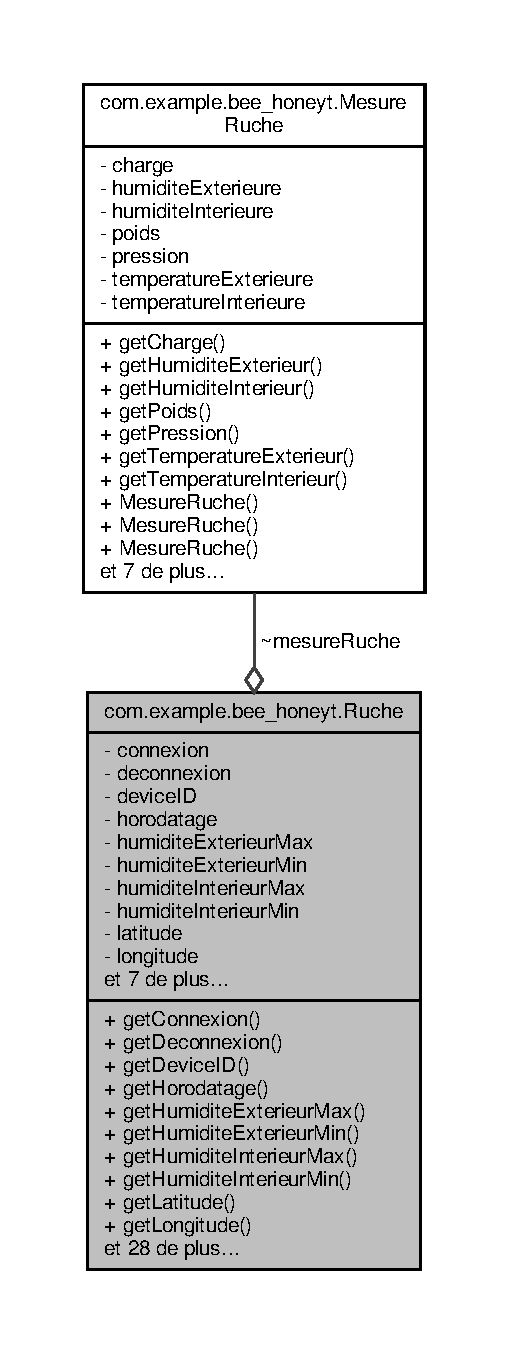
\includegraphics[height=550pt]{classcom_1_1example_1_1bee__honeyt_1_1_ruche__coll__graph}
\end{center}
\end{figure}
\subsubsection*{Fonctions membres publiques}
\begin{DoxyCompactItemize}
\item 
String \hyperlink{classcom_1_1example_1_1bee__honeyt_1_1_ruche_abe485f3c2af62e324ffed32bb84c796f}{get\+Connexion} ()
\item 
String \hyperlink{classcom_1_1example_1_1bee__honeyt_1_1_ruche_a57fc0d510a3e9594e24b6586fcbea9ef}{get\+Deconnexion} ()
\item 
final String \hyperlink{classcom_1_1example_1_1bee__honeyt_1_1_ruche_a4960ba8542f507c850978b939b9aa9e5}{get\+Device\+ID} ()
\item 
String \hyperlink{classcom_1_1example_1_1bee__honeyt_1_1_ruche_a864e48de51e9b0e8e5c78ed7fe58a2d9}{get\+Horodatage} ()
\item 
final double \hyperlink{classcom_1_1example_1_1bee__honeyt_1_1_ruche_ae489d121777412762533465498d1e60c}{get\+Humidite\+Exterieur\+Max} ()
\item 
final double \hyperlink{classcom_1_1example_1_1bee__honeyt_1_1_ruche_a53c9d56abd4eed6f2f2d413e78ab0aba}{get\+Humidite\+Exterieur\+Min} ()
\item 
final double \hyperlink{classcom_1_1example_1_1bee__honeyt_1_1_ruche_a80f34bd8fdc880a8f94d9d61b6b70c78}{get\+Humidite\+Interieur\+Max} ()
\item 
final double \hyperlink{classcom_1_1example_1_1bee__honeyt_1_1_ruche_a4885004ef2c40754789156d83e600b13}{get\+Humidite\+Interieur\+Min} ()
\item 
final double \hyperlink{classcom_1_1example_1_1bee__honeyt_1_1_ruche_a1e291ebb5c69c90fa5b6b7fafe09820e}{get\+Latitude} ()
\item 
final double \hyperlink{classcom_1_1example_1_1bee__honeyt_1_1_ruche_a8a460b9473646a05668426a57e9773cb}{get\+Longitude} ()
\item 
final \hyperlink{classcom_1_1example_1_1bee__honeyt_1_1_mesure_ruche}{Mesure\+Ruche} \hyperlink{classcom_1_1example_1_1bee__honeyt_1_1_ruche_afab94785f8af31f6ce436394ab41c9f3}{get\+Mesure\+Ruche} ()
\item 
final String \hyperlink{classcom_1_1example_1_1bee__honeyt_1_1_ruche_a940047f0b4b8218e7faa7eafcc9665b2}{get\+Nom} ()
\item 
final double \hyperlink{classcom_1_1example_1_1bee__honeyt_1_1_ruche_a713d2985a0a10983ad16d510decf46a3}{get\+Poids\+Max} ()
\item 
final double \hyperlink{classcom_1_1example_1_1bee__honeyt_1_1_ruche_a71764fe95390c37cce877a60c6a630e3}{get\+Poids\+Min} ()
\item 
final double \hyperlink{classcom_1_1example_1_1bee__honeyt_1_1_ruche_a9fbd64d989fba4ae535329192a2396ff}{get\+Temperature\+Exterieur\+Max} ()
\item 
final double \hyperlink{classcom_1_1example_1_1bee__honeyt_1_1_ruche_ada637700d05524a98a143074c43acb7e}{get\+Temperature\+Exterieur\+Min} ()
\item 
final double \hyperlink{classcom_1_1example_1_1bee__honeyt_1_1_ruche_a460323968438c2f0ba77b4d7e92c53bd}{get\+Temperature\+Interieur\+Max} ()
\item 
final double \hyperlink{classcom_1_1example_1_1bee__honeyt_1_1_ruche_a8627a17c2f48ceef15f665065da86255}{get\+Temperature\+Interieur\+Min} ()
\item 
\hyperlink{classcom_1_1example_1_1bee__honeyt_1_1_ruche_aab68c5c3479f1def1b57a4d8b9cca9cd}{Ruche} (String \hyperlink{classcom_1_1example_1_1bee__honeyt_1_1_ruche_ac72094a8a08cf8f485be1456863bc4bd}{nom}, String \hyperlink{classcom_1_1example_1_1bee__honeyt_1_1_ruche_a7126c2ff9e0b3b5365e042c5309ad775}{device\+ID})
\item 
\hyperlink{classcom_1_1example_1_1bee__honeyt_1_1_ruche_ae3747158da62331b68bf99f5b5bab2a6}{Ruche} (String \hyperlink{classcom_1_1example_1_1bee__honeyt_1_1_ruche_ac72094a8a08cf8f485be1456863bc4bd}{nom}, String \hyperlink{classcom_1_1example_1_1bee__honeyt_1_1_ruche_a7126c2ff9e0b3b5365e042c5309ad775}{device\+ID}, String \hyperlink{classcom_1_1example_1_1bee__honeyt_1_1_ruche_a93b3665d844cbba761ebf9a19a1d7d34}{horodatage}, String \hyperlink{classcom_1_1example_1_1bee__honeyt_1_1_ruche_a8b1b18ca9364533f66214ed9daea875e}{connexion}, String \hyperlink{classcom_1_1example_1_1bee__honeyt_1_1_ruche_a91168fb786c93a5233138f67b6a121ad}{deconnexion}, double \hyperlink{classcom_1_1example_1_1bee__honeyt_1_1_ruche_a143b0b293ab3aaa67a86550efeb56f07}{temperature\+Interieur\+Min}, double \hyperlink{classcom_1_1example_1_1bee__honeyt_1_1_ruche_af2d8d214dabc9af08329aa3173047245}{temperature\+Interieur\+Max}, double \hyperlink{classcom_1_1example_1_1bee__honeyt_1_1_ruche_a6e88eae7cc58b7c7ca3846d789fe1c2b}{temperature\+Exterieur\+Min}, double \hyperlink{classcom_1_1example_1_1bee__honeyt_1_1_ruche_afd45ecd796457b633615488195153114}{temperature\+Exterieur\+Max}, double \hyperlink{classcom_1_1example_1_1bee__honeyt_1_1_ruche_ab8234d1bae28a10622b331d3b773445d}{humidite\+Interieur\+Min}, double \hyperlink{classcom_1_1example_1_1bee__honeyt_1_1_ruche_a1483266a1f1ba7d83e0f69bef8e26231}{humidite\+Interieur\+Max}, double \hyperlink{classcom_1_1example_1_1bee__honeyt_1_1_ruche_ad58b8815412827add256f6c6e11d3043}{humidite\+Exterieur\+Min}, double \hyperlink{classcom_1_1example_1_1bee__honeyt_1_1_ruche_a76e636b4d5e0a18b187905e0d6d73a71}{humidite\+Exterieur\+Max}, double \hyperlink{classcom_1_1example_1_1bee__honeyt_1_1_ruche_a3408f099f2fab8700353e6e266fe8221}{poids\+Min}, double \hyperlink{classcom_1_1example_1_1bee__honeyt_1_1_ruche_a5901bf432f6d2de0e5facb8952277cbc}{poids\+Max}, double \hyperlink{classcom_1_1example_1_1bee__honeyt_1_1_ruche_aaeb7392ff8f3f26203e23f1dd57ae89f}{longitude}, double \hyperlink{classcom_1_1example_1_1bee__honeyt_1_1_ruche_a6a75dfabd9812334d502756f91fa4aa9}{latitude})
\item 
\hyperlink{classcom_1_1example_1_1bee__honeyt_1_1_ruche_a30f0d3e27135f5721ef7cd5117235896}{Ruche} (\hyperlink{classcom_1_1example_1_1bee__honeyt_1_1_ruche}{Ruche} ruche)
\item 
void \hyperlink{classcom_1_1example_1_1bee__honeyt_1_1_ruche_a6e1d75a4baf0c9255961bc64f7deca36}{set\+Connexion} ()
\item 
void \hyperlink{classcom_1_1example_1_1bee__honeyt_1_1_ruche_ae247736718ddb17f37e76e0615906091}{set\+Deconnexion} (String \hyperlink{classcom_1_1example_1_1bee__honeyt_1_1_ruche_a91168fb786c93a5233138f67b6a121ad}{deconnexion})
\item 
void \hyperlink{classcom_1_1example_1_1bee__honeyt_1_1_ruche_aff1e1caa39a1d012b1714df3902941f8}{set\+Horodatage} (String \hyperlink{classcom_1_1example_1_1bee__honeyt_1_1_ruche_a93b3665d844cbba761ebf9a19a1d7d34}{horodatage})
\item 
void \hyperlink{classcom_1_1example_1_1bee__honeyt_1_1_ruche_a8ed5f5c7ede5ca2172306b91a0b6c9b7}{set\+Humidite\+Exterieur\+Max} (double \hyperlink{classcom_1_1example_1_1bee__honeyt_1_1_ruche_a76e636b4d5e0a18b187905e0d6d73a71}{humidite\+Exterieur\+Max})
\item 
void \hyperlink{classcom_1_1example_1_1bee__honeyt_1_1_ruche_ab4e0d29d75a71336a51dad3d4f17b758}{set\+Humidite\+Exterieur\+Min} (double \hyperlink{classcom_1_1example_1_1bee__honeyt_1_1_ruche_ad58b8815412827add256f6c6e11d3043}{humidite\+Exterieur\+Min})
\item 
void \hyperlink{classcom_1_1example_1_1bee__honeyt_1_1_ruche_aa17a8858db45900b9087e0f35bdf2e23}{set\+Humidite\+Interieur\+Max} (double \hyperlink{classcom_1_1example_1_1bee__honeyt_1_1_ruche_a1483266a1f1ba7d83e0f69bef8e26231}{humidite\+Interieur\+Max})
\item 
void \hyperlink{classcom_1_1example_1_1bee__honeyt_1_1_ruche_ac06e9c83418f30546fea5d29f250b323}{set\+Humidite\+Interieur\+Min} (double \hyperlink{classcom_1_1example_1_1bee__honeyt_1_1_ruche_ab8234d1bae28a10622b331d3b773445d}{humidite\+Interieur\+Min})
\item 
void \hyperlink{classcom_1_1example_1_1bee__honeyt_1_1_ruche_a38df72556466a10a52a4f3b799722532}{set\+Latitude} (double \hyperlink{classcom_1_1example_1_1bee__honeyt_1_1_ruche_a6a75dfabd9812334d502756f91fa4aa9}{latitude})
\item 
void \hyperlink{classcom_1_1example_1_1bee__honeyt_1_1_ruche_aef8fc612e8ccdabd8234bff9b335925c}{set\+Longitude} (double \hyperlink{classcom_1_1example_1_1bee__honeyt_1_1_ruche_aaeb7392ff8f3f26203e23f1dd57ae89f}{longitude})
\item 
void \hyperlink{classcom_1_1example_1_1bee__honeyt_1_1_ruche_ad98ddabc86442d12acd1047aa746138b}{set\+Mesure\+Ruche} (\hyperlink{classcom_1_1example_1_1bee__honeyt_1_1_mesure_ruche}{Mesure\+Ruche} mesure\+Ruche)
\item 
void \hyperlink{classcom_1_1example_1_1bee__honeyt_1_1_ruche_aae5d95d914d3d2c2e72c4bb9e9ab03f4}{set\+Nom} (String nouveau\+Nom)
\item 
void \hyperlink{classcom_1_1example_1_1bee__honeyt_1_1_ruche_a76fb01b4b1fd90662907635efe949a9e}{set\+Poids\+Max} (double \hyperlink{classcom_1_1example_1_1bee__honeyt_1_1_ruche_a5901bf432f6d2de0e5facb8952277cbc}{poids\+Max})
\item 
void \hyperlink{classcom_1_1example_1_1bee__honeyt_1_1_ruche_aace243242d173adf82592342fecc1328}{set\+Poids\+Min} (double \hyperlink{classcom_1_1example_1_1bee__honeyt_1_1_ruche_a3408f099f2fab8700353e6e266fe8221}{poids\+Min})
\item 
void \hyperlink{classcom_1_1example_1_1bee__honeyt_1_1_ruche_a041d831cfbd058ba27d1b6901b046391}{set\+Temperature\+Exterieur\+Max} (double \hyperlink{classcom_1_1example_1_1bee__honeyt_1_1_ruche_afd45ecd796457b633615488195153114}{temperature\+Exterieur\+Max})
\item 
void \hyperlink{classcom_1_1example_1_1bee__honeyt_1_1_ruche_ab93955d5269feca538027be06711413a}{set\+Temperature\+Exterieur\+Min} (double \hyperlink{classcom_1_1example_1_1bee__honeyt_1_1_ruche_a6e88eae7cc58b7c7ca3846d789fe1c2b}{temperature\+Exterieur\+Min})
\item 
void \hyperlink{classcom_1_1example_1_1bee__honeyt_1_1_ruche_ad0c1bb53162040918c8a9f2ed7c37dd0}{set\+Temperature\+Interieur\+Max} (double \hyperlink{classcom_1_1example_1_1bee__honeyt_1_1_ruche_af2d8d214dabc9af08329aa3173047245}{temperature\+Interieur\+Max})
\item 
void \hyperlink{classcom_1_1example_1_1bee__honeyt_1_1_ruche_abd355743c57f79e2bf544bd20559b33f}{set\+Temperature\+Interieur\+Min} (double \hyperlink{classcom_1_1example_1_1bee__honeyt_1_1_ruche_a143b0b293ab3aaa67a86550efeb56f07}{temperature\+Interieur\+Min})
\end{DoxyCompactItemize}
\subsubsection*{Attributs privés}
\begin{DoxyCompactItemize}
\item 
String \hyperlink{classcom_1_1example_1_1bee__honeyt_1_1_ruche_a8b1b18ca9364533f66214ed9daea875e}{connexion}
\item 
String \hyperlink{classcom_1_1example_1_1bee__honeyt_1_1_ruche_a91168fb786c93a5233138f67b6a121ad}{deconnexion}
\item 
String \hyperlink{classcom_1_1example_1_1bee__honeyt_1_1_ruche_a7126c2ff9e0b3b5365e042c5309ad775}{device\+ID}
\begin{DoxyCompactList}\small\item\em l\textquotesingle{}id de la ruche pour T\+TN \end{DoxyCompactList}\item 
String \hyperlink{classcom_1_1example_1_1bee__honeyt_1_1_ruche_a93b3665d844cbba761ebf9a19a1d7d34}{horodatage}
\item 
double \hyperlink{classcom_1_1example_1_1bee__honeyt_1_1_ruche_a76e636b4d5e0a18b187905e0d6d73a71}{humidite\+Exterieur\+Max} = 0.\+0
\item 
double \hyperlink{classcom_1_1example_1_1bee__honeyt_1_1_ruche_ad58b8815412827add256f6c6e11d3043}{humidite\+Exterieur\+Min} = 0.\+0
\item 
double \hyperlink{classcom_1_1example_1_1bee__honeyt_1_1_ruche_a1483266a1f1ba7d83e0f69bef8e26231}{humidite\+Interieur\+Max} = 0.\+0
\item 
double \hyperlink{classcom_1_1example_1_1bee__honeyt_1_1_ruche_ab8234d1bae28a10622b331d3b773445d}{humidite\+Interieur\+Min} = 0.\+0
\item 
double \hyperlink{classcom_1_1example_1_1bee__honeyt_1_1_ruche_a6a75dfabd9812334d502756f91fa4aa9}{latitude} = 0.\+0
\item 
double \hyperlink{classcom_1_1example_1_1bee__honeyt_1_1_ruche_aaeb7392ff8f3f26203e23f1dd57ae89f}{longitude} = 0.\+0
\item 
String \hyperlink{classcom_1_1example_1_1bee__honeyt_1_1_ruche_ac72094a8a08cf8f485be1456863bc4bd}{nom} = \char`\"{}\char`\"{}
\begin{DoxyCompactList}\small\item\em le nom de la ruche pour l\textquotesingle{}apiculteur \end{DoxyCompactList}\item 
double \hyperlink{classcom_1_1example_1_1bee__honeyt_1_1_ruche_a5901bf432f6d2de0e5facb8952277cbc}{poids\+Max} = 0.\+0
\item 
double \hyperlink{classcom_1_1example_1_1bee__honeyt_1_1_ruche_a3408f099f2fab8700353e6e266fe8221}{poids\+Min} = 0.\+0
\item 
double \hyperlink{classcom_1_1example_1_1bee__honeyt_1_1_ruche_afd45ecd796457b633615488195153114}{temperature\+Exterieur\+Max} = 0.\+0
\item 
double \hyperlink{classcom_1_1example_1_1bee__honeyt_1_1_ruche_a6e88eae7cc58b7c7ca3846d789fe1c2b}{temperature\+Exterieur\+Min} = 0.\+0
\item 
double \hyperlink{classcom_1_1example_1_1bee__honeyt_1_1_ruche_af2d8d214dabc9af08329aa3173047245}{temperature\+Interieur\+Max} = 0.\+0
\item 
double \hyperlink{classcom_1_1example_1_1bee__honeyt_1_1_ruche_a143b0b293ab3aaa67a86550efeb56f07}{temperature\+Interieur\+Min} = 0.\+0
\end{DoxyCompactItemize}


\subsubsection{Description détaillée}
Les données et seuils d\textquotesingle{}une ruche. 

Définition à la ligne \hyperlink{_ruche_8java_source_l00015}{15} du fichier \hyperlink{_ruche_8java_source}{Ruche.\+java}.



\subsubsection{Documentation des constructeurs et destructeur}
\mbox{\Hypertarget{classcom_1_1example_1_1bee__honeyt_1_1_ruche_aab68c5c3479f1def1b57a4d8b9cca9cd}\label{classcom_1_1example_1_1bee__honeyt_1_1_ruche_aab68c5c3479f1def1b57a4d8b9cca9cd}} 
\index{com\+::example\+::bee\+\_\+honeyt\+::\+Ruche@{com\+::example\+::bee\+\_\+honeyt\+::\+Ruche}!Ruche@{Ruche}}
\index{Ruche@{Ruche}!com\+::example\+::bee\+\_\+honeyt\+::\+Ruche@{com\+::example\+::bee\+\_\+honeyt\+::\+Ruche}}
\paragraph{\texorpdfstring{Ruche()}{Ruche()}\hspace{0.1cm}{\footnotesize\ttfamily [1/3]}}
{\footnotesize\ttfamily com.\+example.\+bee\+\_\+honeyt.\+Ruche.\+Ruche (\begin{DoxyParamCaption}\item[{String}]{nom,  }\item[{String}]{device\+ID }\end{DoxyParamCaption})}



Définition à la ligne \hyperlink{_ruche_8java_source_l00038}{38} du fichier \hyperlink{_ruche_8java_source}{Ruche.\+java}.



Références \hyperlink{_ruche_8java_source_l00019}{com.\+example.\+bee\+\_\+honeyt.\+Ruche.\+device\+ID}, et \hyperlink{_ruche_8java_source_l00018}{com.\+example.\+bee\+\_\+honeyt.\+Ruche.\+nom}.


\begin{DoxyCode}
00039     \{
00040         this.\hyperlink{classcom_1_1example_1_1bee__honeyt_1_1_ruche_ac72094a8a08cf8f485be1456863bc4bd}{nom} = \hyperlink{classcom_1_1example_1_1bee__honeyt_1_1_ruche_ac72094a8a08cf8f485be1456863bc4bd}{nom};
00041         this.\hyperlink{classcom_1_1example_1_1bee__honeyt_1_1_ruche_a7126c2ff9e0b3b5365e042c5309ad775}{deviceID} = \hyperlink{classcom_1_1example_1_1bee__honeyt_1_1_ruche_a7126c2ff9e0b3b5365e042c5309ad775}{deviceID};
00042     \}
\end{DoxyCode}
\mbox{\Hypertarget{classcom_1_1example_1_1bee__honeyt_1_1_ruche_ae3747158da62331b68bf99f5b5bab2a6}\label{classcom_1_1example_1_1bee__honeyt_1_1_ruche_ae3747158da62331b68bf99f5b5bab2a6}} 
\index{com\+::example\+::bee\+\_\+honeyt\+::\+Ruche@{com\+::example\+::bee\+\_\+honeyt\+::\+Ruche}!Ruche@{Ruche}}
\index{Ruche@{Ruche}!com\+::example\+::bee\+\_\+honeyt\+::\+Ruche@{com\+::example\+::bee\+\_\+honeyt\+::\+Ruche}}
\paragraph{\texorpdfstring{Ruche()}{Ruche()}\hspace{0.1cm}{\footnotesize\ttfamily [2/3]}}
{\footnotesize\ttfamily com.\+example.\+bee\+\_\+honeyt.\+Ruche.\+Ruche (\begin{DoxyParamCaption}\item[{String}]{nom,  }\item[{String}]{device\+ID,  }\item[{String}]{horodatage,  }\item[{String}]{connexion,  }\item[{String}]{deconnexion,  }\item[{double}]{temperature\+Interieur\+Min,  }\item[{double}]{temperature\+Interieur\+Max,  }\item[{double}]{temperature\+Exterieur\+Min,  }\item[{double}]{temperature\+Exterieur\+Max,  }\item[{double}]{humidite\+Interieur\+Min,  }\item[{double}]{humidite\+Interieur\+Max,  }\item[{double}]{humidite\+Exterieur\+Min,  }\item[{double}]{humidite\+Exterieur\+Max,  }\item[{double}]{poids\+Min,  }\item[{double}]{poids\+Max,  }\item[{double}]{longitude,  }\item[{double}]{latitude }\end{DoxyParamCaption})}



Définition à la ligne \hyperlink{_ruche_8java_source_l00044}{44} du fichier \hyperlink{_ruche_8java_source}{Ruche.\+java}.



Références \hyperlink{_ruche_8java_source_l00021}{com.\+example.\+bee\+\_\+honeyt.\+Ruche.\+connexion}, \hyperlink{_ruche_8java_source_l00022}{com.\+example.\+bee\+\_\+honeyt.\+Ruche.\+deconnexion}, \hyperlink{_ruche_8java_source_l00019}{com.\+example.\+bee\+\_\+honeyt.\+Ruche.\+device\+ID}, \hyperlink{_ruche_8java_source_l00020}{com.\+example.\+bee\+\_\+honeyt.\+Ruche.\+horodatage}, \hyperlink{_ruche_8java_source_l00032}{com.\+example.\+bee\+\_\+honeyt.\+Ruche.\+humidite\+Exterieur\+Max}, \hyperlink{_ruche_8java_source_l00031}{com.\+example.\+bee\+\_\+honeyt.\+Ruche.\+humidite\+Exterieur\+Min}, \hyperlink{_ruche_8java_source_l00030}{com.\+example.\+bee\+\_\+honeyt.\+Ruche.\+humidite\+Interieur\+Max}, \hyperlink{_ruche_8java_source_l00029}{com.\+example.\+bee\+\_\+honeyt.\+Ruche.\+humidite\+Interieur\+Min}, \hyperlink{_ruche_8java_source_l00036}{com.\+example.\+bee\+\_\+honeyt.\+Ruche.\+latitude}, \hyperlink{_ruche_8java_source_l00035}{com.\+example.\+bee\+\_\+honeyt.\+Ruche.\+longitude}, \hyperlink{_ruche_8java_source_l00018}{com.\+example.\+bee\+\_\+honeyt.\+Ruche.\+nom}, \hyperlink{_ruche_8java_source_l00034}{com.\+example.\+bee\+\_\+honeyt.\+Ruche.\+poids\+Max}, \hyperlink{_ruche_8java_source_l00033}{com.\+example.\+bee\+\_\+honeyt.\+Ruche.\+poids\+Min}, \hyperlink{_ruche_8java_source_l00028}{com.\+example.\+bee\+\_\+honeyt.\+Ruche.\+temperature\+Exterieur\+Max}, \hyperlink{_ruche_8java_source_l00027}{com.\+example.\+bee\+\_\+honeyt.\+Ruche.\+temperature\+Exterieur\+Min}, \hyperlink{_ruche_8java_source_l00026}{com.\+example.\+bee\+\_\+honeyt.\+Ruche.\+temperature\+Interieur\+Max}, et \hyperlink{_ruche_8java_source_l00025}{com.\+example.\+bee\+\_\+honeyt.\+Ruche.\+temperature\+Interieur\+Min}.


\begin{DoxyCode}
00048     \{
00049         this.\hyperlink{classcom_1_1example_1_1bee__honeyt_1_1_ruche_ac72094a8a08cf8f485be1456863bc4bd}{nom} = \hyperlink{classcom_1_1example_1_1bee__honeyt_1_1_ruche_ac72094a8a08cf8f485be1456863bc4bd}{nom};
00050         this.\hyperlink{classcom_1_1example_1_1bee__honeyt_1_1_ruche_a7126c2ff9e0b3b5365e042c5309ad775}{deviceID} = \hyperlink{classcom_1_1example_1_1bee__honeyt_1_1_ruche_a7126c2ff9e0b3b5365e042c5309ad775}{deviceID};
00051         this.\hyperlink{classcom_1_1example_1_1bee__honeyt_1_1_ruche_a93b3665d844cbba761ebf9a19a1d7d34}{horodatage} = \hyperlink{classcom_1_1example_1_1bee__honeyt_1_1_ruche_a93b3665d844cbba761ebf9a19a1d7d34}{horodatage};
00052         this.\hyperlink{classcom_1_1example_1_1bee__honeyt_1_1_ruche_a8b1b18ca9364533f66214ed9daea875e}{connexion} = \hyperlink{classcom_1_1example_1_1bee__honeyt_1_1_ruche_a8b1b18ca9364533f66214ed9daea875e}{connexion};
00053         this.\hyperlink{classcom_1_1example_1_1bee__honeyt_1_1_ruche_a91168fb786c93a5233138f67b6a121ad}{deconnexion} = \hyperlink{classcom_1_1example_1_1bee__honeyt_1_1_ruche_a91168fb786c93a5233138f67b6a121ad}{deconnexion};
00054         this.\hyperlink{classcom_1_1example_1_1bee__honeyt_1_1_ruche_a143b0b293ab3aaa67a86550efeb56f07}{temperatureInterieurMin} = 
      \hyperlink{classcom_1_1example_1_1bee__honeyt_1_1_ruche_a143b0b293ab3aaa67a86550efeb56f07}{temperatureInterieurMin};
00055         this.\hyperlink{classcom_1_1example_1_1bee__honeyt_1_1_ruche_af2d8d214dabc9af08329aa3173047245}{temperatureInterieurMax} = 
      \hyperlink{classcom_1_1example_1_1bee__honeyt_1_1_ruche_af2d8d214dabc9af08329aa3173047245}{temperatureInterieurMax};
00056         this.\hyperlink{classcom_1_1example_1_1bee__honeyt_1_1_ruche_a6e88eae7cc58b7c7ca3846d789fe1c2b}{temperatureExterieurMin} = 
      \hyperlink{classcom_1_1example_1_1bee__honeyt_1_1_ruche_a6e88eae7cc58b7c7ca3846d789fe1c2b}{temperatureExterieurMin};
00057         this.\hyperlink{classcom_1_1example_1_1bee__honeyt_1_1_ruche_afd45ecd796457b633615488195153114}{temperatureExterieurMax} = 
      \hyperlink{classcom_1_1example_1_1bee__honeyt_1_1_ruche_afd45ecd796457b633615488195153114}{temperatureExterieurMax};
00058         this.\hyperlink{classcom_1_1example_1_1bee__honeyt_1_1_ruche_ab8234d1bae28a10622b331d3b773445d}{humiditeInterieurMin} = \hyperlink{classcom_1_1example_1_1bee__honeyt_1_1_ruche_ab8234d1bae28a10622b331d3b773445d}{humiditeInterieurMin};
00059         this.\hyperlink{classcom_1_1example_1_1bee__honeyt_1_1_ruche_a1483266a1f1ba7d83e0f69bef8e26231}{humiditeInterieurMax} = \hyperlink{classcom_1_1example_1_1bee__honeyt_1_1_ruche_a1483266a1f1ba7d83e0f69bef8e26231}{humiditeInterieurMax};
00060         this.\hyperlink{classcom_1_1example_1_1bee__honeyt_1_1_ruche_ad58b8815412827add256f6c6e11d3043}{humiditeExterieurMin} = \hyperlink{classcom_1_1example_1_1bee__honeyt_1_1_ruche_ad58b8815412827add256f6c6e11d3043}{humiditeExterieurMin};
00061         this.\hyperlink{classcom_1_1example_1_1bee__honeyt_1_1_ruche_a76e636b4d5e0a18b187905e0d6d73a71}{humiditeExterieurMax} = \hyperlink{classcom_1_1example_1_1bee__honeyt_1_1_ruche_a76e636b4d5e0a18b187905e0d6d73a71}{humiditeExterieurMax};
00062         this.\hyperlink{classcom_1_1example_1_1bee__honeyt_1_1_ruche_a3408f099f2fab8700353e6e266fe8221}{poidsMin} = \hyperlink{classcom_1_1example_1_1bee__honeyt_1_1_ruche_a3408f099f2fab8700353e6e266fe8221}{poidsMin};
00063         this.\hyperlink{classcom_1_1example_1_1bee__honeyt_1_1_ruche_a5901bf432f6d2de0e5facb8952277cbc}{poidsMax} = \hyperlink{classcom_1_1example_1_1bee__honeyt_1_1_ruche_a5901bf432f6d2de0e5facb8952277cbc}{poidsMax};
00064         this.\hyperlink{classcom_1_1example_1_1bee__honeyt_1_1_ruche_aaeb7392ff8f3f26203e23f1dd57ae89f}{longitude} = \hyperlink{classcom_1_1example_1_1bee__honeyt_1_1_ruche_aaeb7392ff8f3f26203e23f1dd57ae89f}{longitude};
00065         this.\hyperlink{classcom_1_1example_1_1bee__honeyt_1_1_ruche_a6a75dfabd9812334d502756f91fa4aa9}{latitude} = \hyperlink{classcom_1_1example_1_1bee__honeyt_1_1_ruche_a6a75dfabd9812334d502756f91fa4aa9}{latitude};
00066     \}
\end{DoxyCode}
\mbox{\Hypertarget{classcom_1_1example_1_1bee__honeyt_1_1_ruche_a30f0d3e27135f5721ef7cd5117235896}\label{classcom_1_1example_1_1bee__honeyt_1_1_ruche_a30f0d3e27135f5721ef7cd5117235896}} 
\index{com\+::example\+::bee\+\_\+honeyt\+::\+Ruche@{com\+::example\+::bee\+\_\+honeyt\+::\+Ruche}!Ruche@{Ruche}}
\index{Ruche@{Ruche}!com\+::example\+::bee\+\_\+honeyt\+::\+Ruche@{com\+::example\+::bee\+\_\+honeyt\+::\+Ruche}}
\paragraph{\texorpdfstring{Ruche()}{Ruche()}\hspace{0.1cm}{\footnotesize\ttfamily [3/3]}}
{\footnotesize\ttfamily com.\+example.\+bee\+\_\+honeyt.\+Ruche.\+Ruche (\begin{DoxyParamCaption}\item[{\hyperlink{classcom_1_1example_1_1bee__honeyt_1_1_ruche}{Ruche}}]{ruche }\end{DoxyParamCaption})}



Définition à la ligne \hyperlink{_ruche_8java_source_l00068}{68} du fichier \hyperlink{_ruche_8java_source}{Ruche.\+java}.



Références \hyperlink{_ruche_8java_source_l00021}{com.\+example.\+bee\+\_\+honeyt.\+Ruche.\+connexion}, \hyperlink{_ruche_8java_source_l00022}{com.\+example.\+bee\+\_\+honeyt.\+Ruche.\+deconnexion}, \hyperlink{_ruche_8java_source_l00019}{com.\+example.\+bee\+\_\+honeyt.\+Ruche.\+device\+ID}, \hyperlink{_ruche_8java_source_l00020}{com.\+example.\+bee\+\_\+honeyt.\+Ruche.\+horodatage}, \hyperlink{_ruche_8java_source_l00032}{com.\+example.\+bee\+\_\+honeyt.\+Ruche.\+humidite\+Exterieur\+Max}, \hyperlink{_ruche_8java_source_l00031}{com.\+example.\+bee\+\_\+honeyt.\+Ruche.\+humidite\+Exterieur\+Min}, \hyperlink{_ruche_8java_source_l00030}{com.\+example.\+bee\+\_\+honeyt.\+Ruche.\+humidite\+Interieur\+Max}, \hyperlink{_ruche_8java_source_l00029}{com.\+example.\+bee\+\_\+honeyt.\+Ruche.\+humidite\+Interieur\+Min}, \hyperlink{_ruche_8java_source_l00036}{com.\+example.\+bee\+\_\+honeyt.\+Ruche.\+latitude}, \hyperlink{_ruche_8java_source_l00035}{com.\+example.\+bee\+\_\+honeyt.\+Ruche.\+longitude}, \hyperlink{_ruche_8java_source_l00018}{com.\+example.\+bee\+\_\+honeyt.\+Ruche.\+nom}, \hyperlink{_ruche_8java_source_l00034}{com.\+example.\+bee\+\_\+honeyt.\+Ruche.\+poids\+Max}, \hyperlink{_ruche_8java_source_l00033}{com.\+example.\+bee\+\_\+honeyt.\+Ruche.\+poids\+Min}, \hyperlink{_ruche_8java_source_l00028}{com.\+example.\+bee\+\_\+honeyt.\+Ruche.\+temperature\+Exterieur\+Max}, \hyperlink{_ruche_8java_source_l00027}{com.\+example.\+bee\+\_\+honeyt.\+Ruche.\+temperature\+Exterieur\+Min}, \hyperlink{_ruche_8java_source_l00026}{com.\+example.\+bee\+\_\+honeyt.\+Ruche.\+temperature\+Interieur\+Max}, et \hyperlink{_ruche_8java_source_l00025}{com.\+example.\+bee\+\_\+honeyt.\+Ruche.\+temperature\+Interieur\+Min}.


\begin{DoxyCode}
00069     \{
00070         this.\hyperlink{classcom_1_1example_1_1bee__honeyt_1_1_ruche_ac72094a8a08cf8f485be1456863bc4bd}{nom} = ruche.nom;
00071         this.\hyperlink{classcom_1_1example_1_1bee__honeyt_1_1_ruche_a7126c2ff9e0b3b5365e042c5309ad775}{deviceID} = ruche.deviceID;
00072         this.\hyperlink{classcom_1_1example_1_1bee__honeyt_1_1_ruche_a93b3665d844cbba761ebf9a19a1d7d34}{horodatage} = ruche.horodatage;
00073         this.\hyperlink{classcom_1_1example_1_1bee__honeyt_1_1_ruche_a8b1b18ca9364533f66214ed9daea875e}{connexion} = ruche.connexion;
00074         this.\hyperlink{classcom_1_1example_1_1bee__honeyt_1_1_ruche_a91168fb786c93a5233138f67b6a121ad}{deconnexion} = ruche.deconnexion;
00075         this.\hyperlink{classcom_1_1example_1_1bee__honeyt_1_1_ruche_a143b0b293ab3aaa67a86550efeb56f07}{temperatureInterieurMin} = ruche.temperatureInterieurMin;
00076         this.\hyperlink{classcom_1_1example_1_1bee__honeyt_1_1_ruche_af2d8d214dabc9af08329aa3173047245}{temperatureInterieurMax} = ruche.temperatureInterieurMax;
00077         this.\hyperlink{classcom_1_1example_1_1bee__honeyt_1_1_ruche_a6e88eae7cc58b7c7ca3846d789fe1c2b}{temperatureExterieurMin} = ruche.temperatureExterieurMin;
00078         this.\hyperlink{classcom_1_1example_1_1bee__honeyt_1_1_ruche_afd45ecd796457b633615488195153114}{temperatureExterieurMax} = ruche.temperatureExterieurMax;
00079         this.\hyperlink{classcom_1_1example_1_1bee__honeyt_1_1_ruche_ab8234d1bae28a10622b331d3b773445d}{humiditeInterieurMin} = ruche.humiditeInterieurMin;
00080         this.\hyperlink{classcom_1_1example_1_1bee__honeyt_1_1_ruche_a1483266a1f1ba7d83e0f69bef8e26231}{humiditeInterieurMax} = ruche.humiditeInterieurMax;
00081         this.\hyperlink{classcom_1_1example_1_1bee__honeyt_1_1_ruche_ad58b8815412827add256f6c6e11d3043}{humiditeExterieurMin} = ruche.humiditeExterieurMin;
00082         this.\hyperlink{classcom_1_1example_1_1bee__honeyt_1_1_ruche_a76e636b4d5e0a18b187905e0d6d73a71}{humiditeExterieurMax} = ruche.humiditeExterieurMax;
00083         this.\hyperlink{classcom_1_1example_1_1bee__honeyt_1_1_ruche_a3408f099f2fab8700353e6e266fe8221}{poidsMin} = ruche.poidsMin;
00084         this.\hyperlink{classcom_1_1example_1_1bee__honeyt_1_1_ruche_a5901bf432f6d2de0e5facb8952277cbc}{poidsMax} = ruche.poidsMax;
00085         this.\hyperlink{classcom_1_1example_1_1bee__honeyt_1_1_ruche_aaeb7392ff8f3f26203e23f1dd57ae89f}{longitude} = ruche.longitude;
00086         this.\hyperlink{classcom_1_1example_1_1bee__honeyt_1_1_ruche_a6a75dfabd9812334d502756f91fa4aa9}{latitude} = ruche.latitude;
00087     \}
\end{DoxyCode}


\subsubsection{Documentation des fonctions membres}
\mbox{\Hypertarget{classcom_1_1example_1_1bee__honeyt_1_1_ruche_abe485f3c2af62e324ffed32bb84c796f}\label{classcom_1_1example_1_1bee__honeyt_1_1_ruche_abe485f3c2af62e324ffed32bb84c796f}} 
\index{com\+::example\+::bee\+\_\+honeyt\+::\+Ruche@{com\+::example\+::bee\+\_\+honeyt\+::\+Ruche}!get\+Connexion@{get\+Connexion}}
\index{get\+Connexion@{get\+Connexion}!com\+::example\+::bee\+\_\+honeyt\+::\+Ruche@{com\+::example\+::bee\+\_\+honeyt\+::\+Ruche}}
\paragraph{\texorpdfstring{get\+Connexion()}{getConnexion()}}
{\footnotesize\ttfamily String com.\+example.\+bee\+\_\+honeyt.\+Ruche.\+get\+Connexion (\begin{DoxyParamCaption}{ }\end{DoxyParamCaption})}



Définition à la ligne \hyperlink{_ruche_8java_source_l00111}{111} du fichier \hyperlink{_ruche_8java_source}{Ruche.\+java}.



Références \hyperlink{_ruche_8java_source_l00021}{com.\+example.\+bee\+\_\+honeyt.\+Ruche.\+connexion}.


\begin{DoxyCode}
00111 \{ \textcolor{keywordflow}{return}  \hyperlink{classcom_1_1example_1_1bee__honeyt_1_1_ruche_a8b1b18ca9364533f66214ed9daea875e}{connexion}; \}
\end{DoxyCode}
\mbox{\Hypertarget{classcom_1_1example_1_1bee__honeyt_1_1_ruche_a57fc0d510a3e9594e24b6586fcbea9ef}\label{classcom_1_1example_1_1bee__honeyt_1_1_ruche_a57fc0d510a3e9594e24b6586fcbea9ef}} 
\index{com\+::example\+::bee\+\_\+honeyt\+::\+Ruche@{com\+::example\+::bee\+\_\+honeyt\+::\+Ruche}!get\+Deconnexion@{get\+Deconnexion}}
\index{get\+Deconnexion@{get\+Deconnexion}!com\+::example\+::bee\+\_\+honeyt\+::\+Ruche@{com\+::example\+::bee\+\_\+honeyt\+::\+Ruche}}
\paragraph{\texorpdfstring{get\+Deconnexion()}{getDeconnexion()}}
{\footnotesize\ttfamily String com.\+example.\+bee\+\_\+honeyt.\+Ruche.\+get\+Deconnexion (\begin{DoxyParamCaption}{ }\end{DoxyParamCaption})}



Définition à la ligne \hyperlink{_ruche_8java_source_l00115}{115} du fichier \hyperlink{_ruche_8java_source}{Ruche.\+java}.



Références \hyperlink{_ruche_8java_source_l00022}{com.\+example.\+bee\+\_\+honeyt.\+Ruche.\+deconnexion}.


\begin{DoxyCode}
00115 \{ \textcolor{keywordflow}{return} \hyperlink{classcom_1_1example_1_1bee__honeyt_1_1_ruche_a91168fb786c93a5233138f67b6a121ad}{deconnexion}; \}
\end{DoxyCode}
\mbox{\Hypertarget{classcom_1_1example_1_1bee__honeyt_1_1_ruche_a4960ba8542f507c850978b939b9aa9e5}\label{classcom_1_1example_1_1bee__honeyt_1_1_ruche_a4960ba8542f507c850978b939b9aa9e5}} 
\index{com\+::example\+::bee\+\_\+honeyt\+::\+Ruche@{com\+::example\+::bee\+\_\+honeyt\+::\+Ruche}!get\+Device\+ID@{get\+Device\+ID}}
\index{get\+Device\+ID@{get\+Device\+ID}!com\+::example\+::bee\+\_\+honeyt\+::\+Ruche@{com\+::example\+::bee\+\_\+honeyt\+::\+Ruche}}
\paragraph{\texorpdfstring{get\+Device\+I\+D()}{getDeviceID()}}
{\footnotesize\ttfamily final String com.\+example.\+bee\+\_\+honeyt.\+Ruche.\+get\+Device\+ID (\begin{DoxyParamCaption}{ }\end{DoxyParamCaption})}



Définition à la ligne \hyperlink{_ruche_8java_source_l00099}{99} du fichier \hyperlink{_ruche_8java_source}{Ruche.\+java}.



Références \hyperlink{_ruche_8java_source_l00019}{com.\+example.\+bee\+\_\+honeyt.\+Ruche.\+device\+ID}.


\begin{DoxyCode}
00100     \{
00101         \textcolor{keywordflow}{return} \hyperlink{classcom_1_1example_1_1bee__honeyt_1_1_ruche_a7126c2ff9e0b3b5365e042c5309ad775}{deviceID};
00102     \}
\end{DoxyCode}
\mbox{\Hypertarget{classcom_1_1example_1_1bee__honeyt_1_1_ruche_a864e48de51e9b0e8e5c78ed7fe58a2d9}\label{classcom_1_1example_1_1bee__honeyt_1_1_ruche_a864e48de51e9b0e8e5c78ed7fe58a2d9}} 
\index{com\+::example\+::bee\+\_\+honeyt\+::\+Ruche@{com\+::example\+::bee\+\_\+honeyt\+::\+Ruche}!get\+Horodatage@{get\+Horodatage}}
\index{get\+Horodatage@{get\+Horodatage}!com\+::example\+::bee\+\_\+honeyt\+::\+Ruche@{com\+::example\+::bee\+\_\+honeyt\+::\+Ruche}}
\paragraph{\texorpdfstring{get\+Horodatage()}{getHorodatage()}}
{\footnotesize\ttfamily String com.\+example.\+bee\+\_\+honeyt.\+Ruche.\+get\+Horodatage (\begin{DoxyParamCaption}{ }\end{DoxyParamCaption})}



Définition à la ligne \hyperlink{_ruche_8java_source_l00104}{104} du fichier \hyperlink{_ruche_8java_source}{Ruche.\+java}.



Références \hyperlink{_ruche_8java_source_l00020}{com.\+example.\+bee\+\_\+honeyt.\+Ruche.\+horodatage}.



Référencé par \hyperlink{_i_h_m_mobile_8java_source_l00170}{com.\+example.\+bee\+\_\+honeyt.\+I\+H\+M\+Mobile.\+initialiser\+Liste\+Ruches()}.


\begin{DoxyCode}
00104 \{ \textcolor{keywordflow}{return} \hyperlink{classcom_1_1example_1_1bee__honeyt_1_1_ruche_a93b3665d844cbba761ebf9a19a1d7d34}{horodatage}; \}
\end{DoxyCode}
\mbox{\Hypertarget{classcom_1_1example_1_1bee__honeyt_1_1_ruche_ae489d121777412762533465498d1e60c}\label{classcom_1_1example_1_1bee__honeyt_1_1_ruche_ae489d121777412762533465498d1e60c}} 
\index{com\+::example\+::bee\+\_\+honeyt\+::\+Ruche@{com\+::example\+::bee\+\_\+honeyt\+::\+Ruche}!get\+Humidite\+Exterieur\+Max@{get\+Humidite\+Exterieur\+Max}}
\index{get\+Humidite\+Exterieur\+Max@{get\+Humidite\+Exterieur\+Max}!com\+::example\+::bee\+\_\+honeyt\+::\+Ruche@{com\+::example\+::bee\+\_\+honeyt\+::\+Ruche}}
\paragraph{\texorpdfstring{get\+Humidite\+Exterieur\+Max()}{getHumiditeExterieurMax()}}
{\footnotesize\ttfamily final double com.\+example.\+bee\+\_\+honeyt.\+Ruche.\+get\+Humidite\+Exterieur\+Max (\begin{DoxyParamCaption}{ }\end{DoxyParamCaption})}



Définition à la ligne \hyperlink{_ruche_8java_source_l00199}{199} du fichier \hyperlink{_ruche_8java_source}{Ruche.\+java}.



Références \hyperlink{_ruche_8java_source_l00032}{com.\+example.\+bee\+\_\+honeyt.\+Ruche.\+humidite\+Exterieur\+Max}.


\begin{DoxyCode}
00200     \{
00201         \textcolor{keywordflow}{return} \hyperlink{classcom_1_1example_1_1bee__honeyt_1_1_ruche_a76e636b4d5e0a18b187905e0d6d73a71}{humiditeExterieurMax};
00202     \}
\end{DoxyCode}
\mbox{\Hypertarget{classcom_1_1example_1_1bee__honeyt_1_1_ruche_a53c9d56abd4eed6f2f2d413e78ab0aba}\label{classcom_1_1example_1_1bee__honeyt_1_1_ruche_a53c9d56abd4eed6f2f2d413e78ab0aba}} 
\index{com\+::example\+::bee\+\_\+honeyt\+::\+Ruche@{com\+::example\+::bee\+\_\+honeyt\+::\+Ruche}!get\+Humidite\+Exterieur\+Min@{get\+Humidite\+Exterieur\+Min}}
\index{get\+Humidite\+Exterieur\+Min@{get\+Humidite\+Exterieur\+Min}!com\+::example\+::bee\+\_\+honeyt\+::\+Ruche@{com\+::example\+::bee\+\_\+honeyt\+::\+Ruche}}
\paragraph{\texorpdfstring{get\+Humidite\+Exterieur\+Min()}{getHumiditeExterieurMin()}}
{\footnotesize\ttfamily final double com.\+example.\+bee\+\_\+honeyt.\+Ruche.\+get\+Humidite\+Exterieur\+Min (\begin{DoxyParamCaption}{ }\end{DoxyParamCaption})}



Définition à la ligne \hyperlink{_ruche_8java_source_l00189}{189} du fichier \hyperlink{_ruche_8java_source}{Ruche.\+java}.



Références \hyperlink{_ruche_8java_source_l00031}{com.\+example.\+bee\+\_\+honeyt.\+Ruche.\+humidite\+Exterieur\+Min}.


\begin{DoxyCode}
00190     \{
00191         \textcolor{keywordflow}{return} \hyperlink{classcom_1_1example_1_1bee__honeyt_1_1_ruche_ad58b8815412827add256f6c6e11d3043}{humiditeExterieurMin};
00192     \}
\end{DoxyCode}
\mbox{\Hypertarget{classcom_1_1example_1_1bee__honeyt_1_1_ruche_a80f34bd8fdc880a8f94d9d61b6b70c78}\label{classcom_1_1example_1_1bee__honeyt_1_1_ruche_a80f34bd8fdc880a8f94d9d61b6b70c78}} 
\index{com\+::example\+::bee\+\_\+honeyt\+::\+Ruche@{com\+::example\+::bee\+\_\+honeyt\+::\+Ruche}!get\+Humidite\+Interieur\+Max@{get\+Humidite\+Interieur\+Max}}
\index{get\+Humidite\+Interieur\+Max@{get\+Humidite\+Interieur\+Max}!com\+::example\+::bee\+\_\+honeyt\+::\+Ruche@{com\+::example\+::bee\+\_\+honeyt\+::\+Ruche}}
\paragraph{\texorpdfstring{get\+Humidite\+Interieur\+Max()}{getHumiditeInterieurMax()}}
{\footnotesize\ttfamily final double com.\+example.\+bee\+\_\+honeyt.\+Ruche.\+get\+Humidite\+Interieur\+Max (\begin{DoxyParamCaption}{ }\end{DoxyParamCaption})}



Définition à la ligne \hyperlink{_ruche_8java_source_l00179}{179} du fichier \hyperlink{_ruche_8java_source}{Ruche.\+java}.



Références \hyperlink{_ruche_8java_source_l00030}{com.\+example.\+bee\+\_\+honeyt.\+Ruche.\+humidite\+Interieur\+Max}.


\begin{DoxyCode}
00180     \{
00181         \textcolor{keywordflow}{return} \hyperlink{classcom_1_1example_1_1bee__honeyt_1_1_ruche_a1483266a1f1ba7d83e0f69bef8e26231}{humiditeInterieurMax};
00182     \}
\end{DoxyCode}
\mbox{\Hypertarget{classcom_1_1example_1_1bee__honeyt_1_1_ruche_a4885004ef2c40754789156d83e600b13}\label{classcom_1_1example_1_1bee__honeyt_1_1_ruche_a4885004ef2c40754789156d83e600b13}} 
\index{com\+::example\+::bee\+\_\+honeyt\+::\+Ruche@{com\+::example\+::bee\+\_\+honeyt\+::\+Ruche}!get\+Humidite\+Interieur\+Min@{get\+Humidite\+Interieur\+Min}}
\index{get\+Humidite\+Interieur\+Min@{get\+Humidite\+Interieur\+Min}!com\+::example\+::bee\+\_\+honeyt\+::\+Ruche@{com\+::example\+::bee\+\_\+honeyt\+::\+Ruche}}
\paragraph{\texorpdfstring{get\+Humidite\+Interieur\+Min()}{getHumiditeInterieurMin()}}
{\footnotesize\ttfamily final double com.\+example.\+bee\+\_\+honeyt.\+Ruche.\+get\+Humidite\+Interieur\+Min (\begin{DoxyParamCaption}{ }\end{DoxyParamCaption})}



Définition à la ligne \hyperlink{_ruche_8java_source_l00169}{169} du fichier \hyperlink{_ruche_8java_source}{Ruche.\+java}.



Références \hyperlink{_ruche_8java_source_l00029}{com.\+example.\+bee\+\_\+honeyt.\+Ruche.\+humidite\+Interieur\+Min}.


\begin{DoxyCode}
00170     \{
00171         \textcolor{keywordflow}{return} \hyperlink{classcom_1_1example_1_1bee__honeyt_1_1_ruche_ab8234d1bae28a10622b331d3b773445d}{humiditeInterieurMin};
00172     \}
\end{DoxyCode}
\mbox{\Hypertarget{classcom_1_1example_1_1bee__honeyt_1_1_ruche_a1e291ebb5c69c90fa5b6b7fafe09820e}\label{classcom_1_1example_1_1bee__honeyt_1_1_ruche_a1e291ebb5c69c90fa5b6b7fafe09820e}} 
\index{com\+::example\+::bee\+\_\+honeyt\+::\+Ruche@{com\+::example\+::bee\+\_\+honeyt\+::\+Ruche}!get\+Latitude@{get\+Latitude}}
\index{get\+Latitude@{get\+Latitude}!com\+::example\+::bee\+\_\+honeyt\+::\+Ruche@{com\+::example\+::bee\+\_\+honeyt\+::\+Ruche}}
\paragraph{\texorpdfstring{get\+Latitude()}{getLatitude()}}
{\footnotesize\ttfamily final double com.\+example.\+bee\+\_\+honeyt.\+Ruche.\+get\+Latitude (\begin{DoxyParamCaption}{ }\end{DoxyParamCaption})}



Définition à la ligne \hyperlink{_ruche_8java_source_l00239}{239} du fichier \hyperlink{_ruche_8java_source}{Ruche.\+java}.



Références \hyperlink{_ruche_8java_source_l00036}{com.\+example.\+bee\+\_\+honeyt.\+Ruche.\+latitude}.


\begin{DoxyCode}
00240     \{
00241         \textcolor{keywordflow}{return} \hyperlink{classcom_1_1example_1_1bee__honeyt_1_1_ruche_a6a75dfabd9812334d502756f91fa4aa9}{latitude};
00242     \}
\end{DoxyCode}
\mbox{\Hypertarget{classcom_1_1example_1_1bee__honeyt_1_1_ruche_a8a460b9473646a05668426a57e9773cb}\label{classcom_1_1example_1_1bee__honeyt_1_1_ruche_a8a460b9473646a05668426a57e9773cb}} 
\index{com\+::example\+::bee\+\_\+honeyt\+::\+Ruche@{com\+::example\+::bee\+\_\+honeyt\+::\+Ruche}!get\+Longitude@{get\+Longitude}}
\index{get\+Longitude@{get\+Longitude}!com\+::example\+::bee\+\_\+honeyt\+::\+Ruche@{com\+::example\+::bee\+\_\+honeyt\+::\+Ruche}}
\paragraph{\texorpdfstring{get\+Longitude()}{getLongitude()}}
{\footnotesize\ttfamily final double com.\+example.\+bee\+\_\+honeyt.\+Ruche.\+get\+Longitude (\begin{DoxyParamCaption}{ }\end{DoxyParamCaption})}



Définition à la ligne \hyperlink{_ruche_8java_source_l00229}{229} du fichier \hyperlink{_ruche_8java_source}{Ruche.\+java}.



Références \hyperlink{_ruche_8java_source_l00035}{com.\+example.\+bee\+\_\+honeyt.\+Ruche.\+longitude}.


\begin{DoxyCode}
00230     \{
00231         \textcolor{keywordflow}{return} \hyperlink{classcom_1_1example_1_1bee__honeyt_1_1_ruche_aaeb7392ff8f3f26203e23f1dd57ae89f}{longitude};
00232     \}
\end{DoxyCode}
\mbox{\Hypertarget{classcom_1_1example_1_1bee__honeyt_1_1_ruche_afab94785f8af31f6ce436394ab41c9f3}\label{classcom_1_1example_1_1bee__honeyt_1_1_ruche_afab94785f8af31f6ce436394ab41c9f3}} 
\index{com\+::example\+::bee\+\_\+honeyt\+::\+Ruche@{com\+::example\+::bee\+\_\+honeyt\+::\+Ruche}!get\+Mesure\+Ruche@{get\+Mesure\+Ruche}}
\index{get\+Mesure\+Ruche@{get\+Mesure\+Ruche}!com\+::example\+::bee\+\_\+honeyt\+::\+Ruche@{com\+::example\+::bee\+\_\+honeyt\+::\+Ruche}}
\paragraph{\texorpdfstring{get\+Mesure\+Ruche()}{getMesureRuche()}}
{\footnotesize\ttfamily final \hyperlink{classcom_1_1example_1_1bee__honeyt_1_1_mesure_ruche}{Mesure\+Ruche} com.\+example.\+bee\+\_\+honeyt.\+Ruche.\+get\+Mesure\+Ruche (\begin{DoxyParamCaption}{ }\end{DoxyParamCaption})}



Définition à la ligne \hyperlink{_ruche_8java_source_l00119}{119} du fichier \hyperlink{_ruche_8java_source}{Ruche.\+java}.



Référencé par \hyperlink{_i_h_m_mobile_8java_source_l00170}{com.\+example.\+bee\+\_\+honeyt.\+I\+H\+M\+Mobile.\+initialiser\+Liste\+Ruches()}, et \hyperlink{_i_h_m_mobile_8java_source_l00374}{com.\+example.\+bee\+\_\+honeyt.\+I\+H\+M\+Mobile.\+traiter\+Message()}.


\begin{DoxyCode}
00120     \{
00121         \textcolor{keywordflow}{return} mesureRuche;
00122     \}
\end{DoxyCode}
\mbox{\Hypertarget{classcom_1_1example_1_1bee__honeyt_1_1_ruche_a940047f0b4b8218e7faa7eafcc9665b2}\label{classcom_1_1example_1_1bee__honeyt_1_1_ruche_a940047f0b4b8218e7faa7eafcc9665b2}} 
\index{com\+::example\+::bee\+\_\+honeyt\+::\+Ruche@{com\+::example\+::bee\+\_\+honeyt\+::\+Ruche}!get\+Nom@{get\+Nom}}
\index{get\+Nom@{get\+Nom}!com\+::example\+::bee\+\_\+honeyt\+::\+Ruche@{com\+::example\+::bee\+\_\+honeyt\+::\+Ruche}}
\paragraph{\texorpdfstring{get\+Nom()}{getNom()}}
{\footnotesize\ttfamily final String com.\+example.\+bee\+\_\+honeyt.\+Ruche.\+get\+Nom (\begin{DoxyParamCaption}{ }\end{DoxyParamCaption})}



Définition à la ligne \hyperlink{_ruche_8java_source_l00089}{89} du fichier \hyperlink{_ruche_8java_source}{Ruche.\+java}.



Références \hyperlink{_ruche_8java_source_l00018}{com.\+example.\+bee\+\_\+honeyt.\+Ruche.\+nom}.


\begin{DoxyCode}
00090     \{
00091         \textcolor{keywordflow}{return} \hyperlink{classcom_1_1example_1_1bee__honeyt_1_1_ruche_ac72094a8a08cf8f485be1456863bc4bd}{nom};
00092     \}
\end{DoxyCode}
\mbox{\Hypertarget{classcom_1_1example_1_1bee__honeyt_1_1_ruche_a713d2985a0a10983ad16d510decf46a3}\label{classcom_1_1example_1_1bee__honeyt_1_1_ruche_a713d2985a0a10983ad16d510decf46a3}} 
\index{com\+::example\+::bee\+\_\+honeyt\+::\+Ruche@{com\+::example\+::bee\+\_\+honeyt\+::\+Ruche}!get\+Poids\+Max@{get\+Poids\+Max}}
\index{get\+Poids\+Max@{get\+Poids\+Max}!com\+::example\+::bee\+\_\+honeyt\+::\+Ruche@{com\+::example\+::bee\+\_\+honeyt\+::\+Ruche}}
\paragraph{\texorpdfstring{get\+Poids\+Max()}{getPoidsMax()}}
{\footnotesize\ttfamily final double com.\+example.\+bee\+\_\+honeyt.\+Ruche.\+get\+Poids\+Max (\begin{DoxyParamCaption}{ }\end{DoxyParamCaption})}



Définition à la ligne \hyperlink{_ruche_8java_source_l00219}{219} du fichier \hyperlink{_ruche_8java_source}{Ruche.\+java}.



Références \hyperlink{_ruche_8java_source_l00034}{com.\+example.\+bee\+\_\+honeyt.\+Ruche.\+poids\+Max}.


\begin{DoxyCode}
00220     \{
00221         \textcolor{keywordflow}{return} \hyperlink{classcom_1_1example_1_1bee__honeyt_1_1_ruche_a5901bf432f6d2de0e5facb8952277cbc}{poidsMax};
00222     \}
\end{DoxyCode}
\mbox{\Hypertarget{classcom_1_1example_1_1bee__honeyt_1_1_ruche_a71764fe95390c37cce877a60c6a630e3}\label{classcom_1_1example_1_1bee__honeyt_1_1_ruche_a71764fe95390c37cce877a60c6a630e3}} 
\index{com\+::example\+::bee\+\_\+honeyt\+::\+Ruche@{com\+::example\+::bee\+\_\+honeyt\+::\+Ruche}!get\+Poids\+Min@{get\+Poids\+Min}}
\index{get\+Poids\+Min@{get\+Poids\+Min}!com\+::example\+::bee\+\_\+honeyt\+::\+Ruche@{com\+::example\+::bee\+\_\+honeyt\+::\+Ruche}}
\paragraph{\texorpdfstring{get\+Poids\+Min()}{getPoidsMin()}}
{\footnotesize\ttfamily final double com.\+example.\+bee\+\_\+honeyt.\+Ruche.\+get\+Poids\+Min (\begin{DoxyParamCaption}{ }\end{DoxyParamCaption})}



Définition à la ligne \hyperlink{_ruche_8java_source_l00209}{209} du fichier \hyperlink{_ruche_8java_source}{Ruche.\+java}.



Références \hyperlink{_ruche_8java_source_l00033}{com.\+example.\+bee\+\_\+honeyt.\+Ruche.\+poids\+Min}.


\begin{DoxyCode}
00210     \{
00211         \textcolor{keywordflow}{return} \hyperlink{classcom_1_1example_1_1bee__honeyt_1_1_ruche_a3408f099f2fab8700353e6e266fe8221}{poidsMin};
00212     \}
\end{DoxyCode}
\mbox{\Hypertarget{classcom_1_1example_1_1bee__honeyt_1_1_ruche_a9fbd64d989fba4ae535329192a2396ff}\label{classcom_1_1example_1_1bee__honeyt_1_1_ruche_a9fbd64d989fba4ae535329192a2396ff}} 
\index{com\+::example\+::bee\+\_\+honeyt\+::\+Ruche@{com\+::example\+::bee\+\_\+honeyt\+::\+Ruche}!get\+Temperature\+Exterieur\+Max@{get\+Temperature\+Exterieur\+Max}}
\index{get\+Temperature\+Exterieur\+Max@{get\+Temperature\+Exterieur\+Max}!com\+::example\+::bee\+\_\+honeyt\+::\+Ruche@{com\+::example\+::bee\+\_\+honeyt\+::\+Ruche}}
\paragraph{\texorpdfstring{get\+Temperature\+Exterieur\+Max()}{getTemperatureExterieurMax()}}
{\footnotesize\ttfamily final double com.\+example.\+bee\+\_\+honeyt.\+Ruche.\+get\+Temperature\+Exterieur\+Max (\begin{DoxyParamCaption}{ }\end{DoxyParamCaption})}



Définition à la ligne \hyperlink{_ruche_8java_source_l00159}{159} du fichier \hyperlink{_ruche_8java_source}{Ruche.\+java}.



Références \hyperlink{_ruche_8java_source_l00028}{com.\+example.\+bee\+\_\+honeyt.\+Ruche.\+temperature\+Exterieur\+Max}.


\begin{DoxyCode}
00160     \{
00161         \textcolor{keywordflow}{return} \hyperlink{classcom_1_1example_1_1bee__honeyt_1_1_ruche_afd45ecd796457b633615488195153114}{temperatureExterieurMax};
00162     \}
\end{DoxyCode}
\mbox{\Hypertarget{classcom_1_1example_1_1bee__honeyt_1_1_ruche_ada637700d05524a98a143074c43acb7e}\label{classcom_1_1example_1_1bee__honeyt_1_1_ruche_ada637700d05524a98a143074c43acb7e}} 
\index{com\+::example\+::bee\+\_\+honeyt\+::\+Ruche@{com\+::example\+::bee\+\_\+honeyt\+::\+Ruche}!get\+Temperature\+Exterieur\+Min@{get\+Temperature\+Exterieur\+Min}}
\index{get\+Temperature\+Exterieur\+Min@{get\+Temperature\+Exterieur\+Min}!com\+::example\+::bee\+\_\+honeyt\+::\+Ruche@{com\+::example\+::bee\+\_\+honeyt\+::\+Ruche}}
\paragraph{\texorpdfstring{get\+Temperature\+Exterieur\+Min()}{getTemperatureExterieurMin()}}
{\footnotesize\ttfamily final double com.\+example.\+bee\+\_\+honeyt.\+Ruche.\+get\+Temperature\+Exterieur\+Min (\begin{DoxyParamCaption}{ }\end{DoxyParamCaption})}



Définition à la ligne \hyperlink{_ruche_8java_source_l00149}{149} du fichier \hyperlink{_ruche_8java_source}{Ruche.\+java}.



Références \hyperlink{_ruche_8java_source_l00027}{com.\+example.\+bee\+\_\+honeyt.\+Ruche.\+temperature\+Exterieur\+Min}.


\begin{DoxyCode}
00150     \{
00151         \textcolor{keywordflow}{return} \hyperlink{classcom_1_1example_1_1bee__honeyt_1_1_ruche_a6e88eae7cc58b7c7ca3846d789fe1c2b}{temperatureExterieurMin};
00152     \}
\end{DoxyCode}
\mbox{\Hypertarget{classcom_1_1example_1_1bee__honeyt_1_1_ruche_a460323968438c2f0ba77b4d7e92c53bd}\label{classcom_1_1example_1_1bee__honeyt_1_1_ruche_a460323968438c2f0ba77b4d7e92c53bd}} 
\index{com\+::example\+::bee\+\_\+honeyt\+::\+Ruche@{com\+::example\+::bee\+\_\+honeyt\+::\+Ruche}!get\+Temperature\+Interieur\+Max@{get\+Temperature\+Interieur\+Max}}
\index{get\+Temperature\+Interieur\+Max@{get\+Temperature\+Interieur\+Max}!com\+::example\+::bee\+\_\+honeyt\+::\+Ruche@{com\+::example\+::bee\+\_\+honeyt\+::\+Ruche}}
\paragraph{\texorpdfstring{get\+Temperature\+Interieur\+Max()}{getTemperatureInterieurMax()}}
{\footnotesize\ttfamily final double com.\+example.\+bee\+\_\+honeyt.\+Ruche.\+get\+Temperature\+Interieur\+Max (\begin{DoxyParamCaption}{ }\end{DoxyParamCaption})}



Définition à la ligne \hyperlink{_ruche_8java_source_l00139}{139} du fichier \hyperlink{_ruche_8java_source}{Ruche.\+java}.



Références \hyperlink{_ruche_8java_source_l00026}{com.\+example.\+bee\+\_\+honeyt.\+Ruche.\+temperature\+Interieur\+Max}.


\begin{DoxyCode}
00140     \{
00141         \textcolor{keywordflow}{return} \hyperlink{classcom_1_1example_1_1bee__honeyt_1_1_ruche_af2d8d214dabc9af08329aa3173047245}{temperatureInterieurMax};
00142     \}
\end{DoxyCode}
\mbox{\Hypertarget{classcom_1_1example_1_1bee__honeyt_1_1_ruche_a8627a17c2f48ceef15f665065da86255}\label{classcom_1_1example_1_1bee__honeyt_1_1_ruche_a8627a17c2f48ceef15f665065da86255}} 
\index{com\+::example\+::bee\+\_\+honeyt\+::\+Ruche@{com\+::example\+::bee\+\_\+honeyt\+::\+Ruche}!get\+Temperature\+Interieur\+Min@{get\+Temperature\+Interieur\+Min}}
\index{get\+Temperature\+Interieur\+Min@{get\+Temperature\+Interieur\+Min}!com\+::example\+::bee\+\_\+honeyt\+::\+Ruche@{com\+::example\+::bee\+\_\+honeyt\+::\+Ruche}}
\paragraph{\texorpdfstring{get\+Temperature\+Interieur\+Min()}{getTemperatureInterieurMin()}}
{\footnotesize\ttfamily final double com.\+example.\+bee\+\_\+honeyt.\+Ruche.\+get\+Temperature\+Interieur\+Min (\begin{DoxyParamCaption}{ }\end{DoxyParamCaption})}



Définition à la ligne \hyperlink{_ruche_8java_source_l00129}{129} du fichier \hyperlink{_ruche_8java_source}{Ruche.\+java}.



Références \hyperlink{_ruche_8java_source_l00025}{com.\+example.\+bee\+\_\+honeyt.\+Ruche.\+temperature\+Interieur\+Min}.


\begin{DoxyCode}
00130     \{
00131         \textcolor{keywordflow}{return} \hyperlink{classcom_1_1example_1_1bee__honeyt_1_1_ruche_a143b0b293ab3aaa67a86550efeb56f07}{temperatureInterieurMin};
00132     \}
\end{DoxyCode}
\mbox{\Hypertarget{classcom_1_1example_1_1bee__honeyt_1_1_ruche_a6e1d75a4baf0c9255961bc64f7deca36}\label{classcom_1_1example_1_1bee__honeyt_1_1_ruche_a6e1d75a4baf0c9255961bc64f7deca36}} 
\index{com\+::example\+::bee\+\_\+honeyt\+::\+Ruche@{com\+::example\+::bee\+\_\+honeyt\+::\+Ruche}!set\+Connexion@{set\+Connexion}}
\index{set\+Connexion@{set\+Connexion}!com\+::example\+::bee\+\_\+honeyt\+::\+Ruche@{com\+::example\+::bee\+\_\+honeyt\+::\+Ruche}}
\paragraph{\texorpdfstring{set\+Connexion()}{setConnexion()}}
{\footnotesize\ttfamily void com.\+example.\+bee\+\_\+honeyt.\+Ruche.\+set\+Connexion (\begin{DoxyParamCaption}{ }\end{DoxyParamCaption})}



Définition à la ligne \hyperlink{_ruche_8java_source_l00113}{113} du fichier \hyperlink{_ruche_8java_source}{Ruche.\+java}.



Références \hyperlink{_ruche_8java_source_l00021}{com.\+example.\+bee\+\_\+honeyt.\+Ruche.\+connexion}.


\begin{DoxyCode}
00113 \{ this.\hyperlink{classcom_1_1example_1_1bee__honeyt_1_1_ruche_a8b1b18ca9364533f66214ed9daea875e}{connexion} = \hyperlink{classcom_1_1example_1_1bee__honeyt_1_1_ruche_a8b1b18ca9364533f66214ed9daea875e}{connexion}; \}
\end{DoxyCode}
\mbox{\Hypertarget{classcom_1_1example_1_1bee__honeyt_1_1_ruche_ae247736718ddb17f37e76e0615906091}\label{classcom_1_1example_1_1bee__honeyt_1_1_ruche_ae247736718ddb17f37e76e0615906091}} 
\index{com\+::example\+::bee\+\_\+honeyt\+::\+Ruche@{com\+::example\+::bee\+\_\+honeyt\+::\+Ruche}!set\+Deconnexion@{set\+Deconnexion}}
\index{set\+Deconnexion@{set\+Deconnexion}!com\+::example\+::bee\+\_\+honeyt\+::\+Ruche@{com\+::example\+::bee\+\_\+honeyt\+::\+Ruche}}
\paragraph{\texorpdfstring{set\+Deconnexion()}{setDeconnexion()}}
{\footnotesize\ttfamily void com.\+example.\+bee\+\_\+honeyt.\+Ruche.\+set\+Deconnexion (\begin{DoxyParamCaption}\item[{String}]{deconnexion }\end{DoxyParamCaption})}



Définition à la ligne \hyperlink{_ruche_8java_source_l00117}{117} du fichier \hyperlink{_ruche_8java_source}{Ruche.\+java}.



Références \hyperlink{_ruche_8java_source_l00022}{com.\+example.\+bee\+\_\+honeyt.\+Ruche.\+deconnexion}.


\begin{DoxyCode}
00117 \{ this.\hyperlink{classcom_1_1example_1_1bee__honeyt_1_1_ruche_a91168fb786c93a5233138f67b6a121ad}{deconnexion} = \hyperlink{classcom_1_1example_1_1bee__honeyt_1_1_ruche_a91168fb786c93a5233138f67b6a121ad}{deconnexion}; \}
\end{DoxyCode}
\mbox{\Hypertarget{classcom_1_1example_1_1bee__honeyt_1_1_ruche_aff1e1caa39a1d012b1714df3902941f8}\label{classcom_1_1example_1_1bee__honeyt_1_1_ruche_aff1e1caa39a1d012b1714df3902941f8}} 
\index{com\+::example\+::bee\+\_\+honeyt\+::\+Ruche@{com\+::example\+::bee\+\_\+honeyt\+::\+Ruche}!set\+Horodatage@{set\+Horodatage}}
\index{set\+Horodatage@{set\+Horodatage}!com\+::example\+::bee\+\_\+honeyt\+::\+Ruche@{com\+::example\+::bee\+\_\+honeyt\+::\+Ruche}}
\paragraph{\texorpdfstring{set\+Horodatage()}{setHorodatage()}}
{\footnotesize\ttfamily void com.\+example.\+bee\+\_\+honeyt.\+Ruche.\+set\+Horodatage (\begin{DoxyParamCaption}\item[{String}]{horodatage }\end{DoxyParamCaption})}



Définition à la ligne \hyperlink{_ruche_8java_source_l00106}{106} du fichier \hyperlink{_ruche_8java_source}{Ruche.\+java}.



Références \hyperlink{_ruche_8java_source_l00020}{com.\+example.\+bee\+\_\+honeyt.\+Ruche.\+horodatage}.



Référencé par \hyperlink{_i_h_m_mobile_8java_source_l00374}{com.\+example.\+bee\+\_\+honeyt.\+I\+H\+M\+Mobile.\+traiter\+Message()}.


\begin{DoxyCode}
00107     \{
00108         this.\hyperlink{classcom_1_1example_1_1bee__honeyt_1_1_ruche_a93b3665d844cbba761ebf9a19a1d7d34}{horodatage} = \hyperlink{classcom_1_1example_1_1bee__honeyt_1_1_ruche_a93b3665d844cbba761ebf9a19a1d7d34}{horodatage};
00109     \}
\end{DoxyCode}
\mbox{\Hypertarget{classcom_1_1example_1_1bee__honeyt_1_1_ruche_a8ed5f5c7ede5ca2172306b91a0b6c9b7}\label{classcom_1_1example_1_1bee__honeyt_1_1_ruche_a8ed5f5c7ede5ca2172306b91a0b6c9b7}} 
\index{com\+::example\+::bee\+\_\+honeyt\+::\+Ruche@{com\+::example\+::bee\+\_\+honeyt\+::\+Ruche}!set\+Humidite\+Exterieur\+Max@{set\+Humidite\+Exterieur\+Max}}
\index{set\+Humidite\+Exterieur\+Max@{set\+Humidite\+Exterieur\+Max}!com\+::example\+::bee\+\_\+honeyt\+::\+Ruche@{com\+::example\+::bee\+\_\+honeyt\+::\+Ruche}}
\paragraph{\texorpdfstring{set\+Humidite\+Exterieur\+Max()}{setHumiditeExterieurMax()}}
{\footnotesize\ttfamily void com.\+example.\+bee\+\_\+honeyt.\+Ruche.\+set\+Humidite\+Exterieur\+Max (\begin{DoxyParamCaption}\item[{double}]{humidite\+Exterieur\+Max }\end{DoxyParamCaption})}



Définition à la ligne \hyperlink{_ruche_8java_source_l00204}{204} du fichier \hyperlink{_ruche_8java_source}{Ruche.\+java}.



Références \hyperlink{_ruche_8java_source_l00032}{com.\+example.\+bee\+\_\+honeyt.\+Ruche.\+humidite\+Exterieur\+Max}.


\begin{DoxyCode}
00205     \{
00206         this.\hyperlink{classcom_1_1example_1_1bee__honeyt_1_1_ruche_a76e636b4d5e0a18b187905e0d6d73a71}{humiditeExterieurMax} = \hyperlink{classcom_1_1example_1_1bee__honeyt_1_1_ruche_a76e636b4d5e0a18b187905e0d6d73a71}{humiditeExterieurMax};
00207     \}
\end{DoxyCode}
\mbox{\Hypertarget{classcom_1_1example_1_1bee__honeyt_1_1_ruche_ab4e0d29d75a71336a51dad3d4f17b758}\label{classcom_1_1example_1_1bee__honeyt_1_1_ruche_ab4e0d29d75a71336a51dad3d4f17b758}} 
\index{com\+::example\+::bee\+\_\+honeyt\+::\+Ruche@{com\+::example\+::bee\+\_\+honeyt\+::\+Ruche}!set\+Humidite\+Exterieur\+Min@{set\+Humidite\+Exterieur\+Min}}
\index{set\+Humidite\+Exterieur\+Min@{set\+Humidite\+Exterieur\+Min}!com\+::example\+::bee\+\_\+honeyt\+::\+Ruche@{com\+::example\+::bee\+\_\+honeyt\+::\+Ruche}}
\paragraph{\texorpdfstring{set\+Humidite\+Exterieur\+Min()}{setHumiditeExterieurMin()}}
{\footnotesize\ttfamily void com.\+example.\+bee\+\_\+honeyt.\+Ruche.\+set\+Humidite\+Exterieur\+Min (\begin{DoxyParamCaption}\item[{double}]{humidite\+Exterieur\+Min }\end{DoxyParamCaption})}



Définition à la ligne \hyperlink{_ruche_8java_source_l00194}{194} du fichier \hyperlink{_ruche_8java_source}{Ruche.\+java}.



Références \hyperlink{_ruche_8java_source_l00031}{com.\+example.\+bee\+\_\+honeyt.\+Ruche.\+humidite\+Exterieur\+Min}.


\begin{DoxyCode}
00195     \{
00196         this.\hyperlink{classcom_1_1example_1_1bee__honeyt_1_1_ruche_ad58b8815412827add256f6c6e11d3043}{humiditeExterieurMin} = \hyperlink{classcom_1_1example_1_1bee__honeyt_1_1_ruche_ad58b8815412827add256f6c6e11d3043}{humiditeExterieurMin};
00197     \}
\end{DoxyCode}
\mbox{\Hypertarget{classcom_1_1example_1_1bee__honeyt_1_1_ruche_aa17a8858db45900b9087e0f35bdf2e23}\label{classcom_1_1example_1_1bee__honeyt_1_1_ruche_aa17a8858db45900b9087e0f35bdf2e23}} 
\index{com\+::example\+::bee\+\_\+honeyt\+::\+Ruche@{com\+::example\+::bee\+\_\+honeyt\+::\+Ruche}!set\+Humidite\+Interieur\+Max@{set\+Humidite\+Interieur\+Max}}
\index{set\+Humidite\+Interieur\+Max@{set\+Humidite\+Interieur\+Max}!com\+::example\+::bee\+\_\+honeyt\+::\+Ruche@{com\+::example\+::bee\+\_\+honeyt\+::\+Ruche}}
\paragraph{\texorpdfstring{set\+Humidite\+Interieur\+Max()}{setHumiditeInterieurMax()}}
{\footnotesize\ttfamily void com.\+example.\+bee\+\_\+honeyt.\+Ruche.\+set\+Humidite\+Interieur\+Max (\begin{DoxyParamCaption}\item[{double}]{humidite\+Interieur\+Max }\end{DoxyParamCaption})}



Définition à la ligne \hyperlink{_ruche_8java_source_l00184}{184} du fichier \hyperlink{_ruche_8java_source}{Ruche.\+java}.



Références \hyperlink{_ruche_8java_source_l00030}{com.\+example.\+bee\+\_\+honeyt.\+Ruche.\+humidite\+Interieur\+Max}.


\begin{DoxyCode}
00185     \{
00186         this.\hyperlink{classcom_1_1example_1_1bee__honeyt_1_1_ruche_a1483266a1f1ba7d83e0f69bef8e26231}{humiditeInterieurMax} = \hyperlink{classcom_1_1example_1_1bee__honeyt_1_1_ruche_a1483266a1f1ba7d83e0f69bef8e26231}{humiditeInterieurMax};
00187     \}
\end{DoxyCode}
\mbox{\Hypertarget{classcom_1_1example_1_1bee__honeyt_1_1_ruche_ac06e9c83418f30546fea5d29f250b323}\label{classcom_1_1example_1_1bee__honeyt_1_1_ruche_ac06e9c83418f30546fea5d29f250b323}} 
\index{com\+::example\+::bee\+\_\+honeyt\+::\+Ruche@{com\+::example\+::bee\+\_\+honeyt\+::\+Ruche}!set\+Humidite\+Interieur\+Min@{set\+Humidite\+Interieur\+Min}}
\index{set\+Humidite\+Interieur\+Min@{set\+Humidite\+Interieur\+Min}!com\+::example\+::bee\+\_\+honeyt\+::\+Ruche@{com\+::example\+::bee\+\_\+honeyt\+::\+Ruche}}
\paragraph{\texorpdfstring{set\+Humidite\+Interieur\+Min()}{setHumiditeInterieurMin()}}
{\footnotesize\ttfamily void com.\+example.\+bee\+\_\+honeyt.\+Ruche.\+set\+Humidite\+Interieur\+Min (\begin{DoxyParamCaption}\item[{double}]{humidite\+Interieur\+Min }\end{DoxyParamCaption})}



Définition à la ligne \hyperlink{_ruche_8java_source_l00174}{174} du fichier \hyperlink{_ruche_8java_source}{Ruche.\+java}.



Références \hyperlink{_ruche_8java_source_l00029}{com.\+example.\+bee\+\_\+honeyt.\+Ruche.\+humidite\+Interieur\+Min}.


\begin{DoxyCode}
00175     \{
00176         this.\hyperlink{classcom_1_1example_1_1bee__honeyt_1_1_ruche_ab8234d1bae28a10622b331d3b773445d}{humiditeInterieurMin} = \hyperlink{classcom_1_1example_1_1bee__honeyt_1_1_ruche_ab8234d1bae28a10622b331d3b773445d}{humiditeInterieurMin};
00177     \}
\end{DoxyCode}
\mbox{\Hypertarget{classcom_1_1example_1_1bee__honeyt_1_1_ruche_a38df72556466a10a52a4f3b799722532}\label{classcom_1_1example_1_1bee__honeyt_1_1_ruche_a38df72556466a10a52a4f3b799722532}} 
\index{com\+::example\+::bee\+\_\+honeyt\+::\+Ruche@{com\+::example\+::bee\+\_\+honeyt\+::\+Ruche}!set\+Latitude@{set\+Latitude}}
\index{set\+Latitude@{set\+Latitude}!com\+::example\+::bee\+\_\+honeyt\+::\+Ruche@{com\+::example\+::bee\+\_\+honeyt\+::\+Ruche}}
\paragraph{\texorpdfstring{set\+Latitude()}{setLatitude()}}
{\footnotesize\ttfamily void com.\+example.\+bee\+\_\+honeyt.\+Ruche.\+set\+Latitude (\begin{DoxyParamCaption}\item[{double}]{latitude }\end{DoxyParamCaption})}



Définition à la ligne \hyperlink{_ruche_8java_source_l00244}{244} du fichier \hyperlink{_ruche_8java_source}{Ruche.\+java}.



Références \hyperlink{_ruche_8java_source_l00036}{com.\+example.\+bee\+\_\+honeyt.\+Ruche.\+latitude}.


\begin{DoxyCode}
00245     \{
00246         this.\hyperlink{classcom_1_1example_1_1bee__honeyt_1_1_ruche_a6a75dfabd9812334d502756f91fa4aa9}{latitude} = \hyperlink{classcom_1_1example_1_1bee__honeyt_1_1_ruche_a6a75dfabd9812334d502756f91fa4aa9}{latitude};
00247     \}
\end{DoxyCode}
\mbox{\Hypertarget{classcom_1_1example_1_1bee__honeyt_1_1_ruche_aef8fc612e8ccdabd8234bff9b335925c}\label{classcom_1_1example_1_1bee__honeyt_1_1_ruche_aef8fc612e8ccdabd8234bff9b335925c}} 
\index{com\+::example\+::bee\+\_\+honeyt\+::\+Ruche@{com\+::example\+::bee\+\_\+honeyt\+::\+Ruche}!set\+Longitude@{set\+Longitude}}
\index{set\+Longitude@{set\+Longitude}!com\+::example\+::bee\+\_\+honeyt\+::\+Ruche@{com\+::example\+::bee\+\_\+honeyt\+::\+Ruche}}
\paragraph{\texorpdfstring{set\+Longitude()}{setLongitude()}}
{\footnotesize\ttfamily void com.\+example.\+bee\+\_\+honeyt.\+Ruche.\+set\+Longitude (\begin{DoxyParamCaption}\item[{double}]{longitude }\end{DoxyParamCaption})}



Définition à la ligne \hyperlink{_ruche_8java_source_l00234}{234} du fichier \hyperlink{_ruche_8java_source}{Ruche.\+java}.



Références \hyperlink{_ruche_8java_source_l00035}{com.\+example.\+bee\+\_\+honeyt.\+Ruche.\+longitude}.


\begin{DoxyCode}
00235     \{
00236         this.\hyperlink{classcom_1_1example_1_1bee__honeyt_1_1_ruche_aaeb7392ff8f3f26203e23f1dd57ae89f}{longitude} = \hyperlink{classcom_1_1example_1_1bee__honeyt_1_1_ruche_aaeb7392ff8f3f26203e23f1dd57ae89f}{longitude};
00237     \}
\end{DoxyCode}
\mbox{\Hypertarget{classcom_1_1example_1_1bee__honeyt_1_1_ruche_ad98ddabc86442d12acd1047aa746138b}\label{classcom_1_1example_1_1bee__honeyt_1_1_ruche_ad98ddabc86442d12acd1047aa746138b}} 
\index{com\+::example\+::bee\+\_\+honeyt\+::\+Ruche@{com\+::example\+::bee\+\_\+honeyt\+::\+Ruche}!set\+Mesure\+Ruche@{set\+Mesure\+Ruche}}
\index{set\+Mesure\+Ruche@{set\+Mesure\+Ruche}!com\+::example\+::bee\+\_\+honeyt\+::\+Ruche@{com\+::example\+::bee\+\_\+honeyt\+::\+Ruche}}
\paragraph{\texorpdfstring{set\+Mesure\+Ruche()}{setMesureRuche()}}
{\footnotesize\ttfamily void com.\+example.\+bee\+\_\+honeyt.\+Ruche.\+set\+Mesure\+Ruche (\begin{DoxyParamCaption}\item[{\hyperlink{classcom_1_1example_1_1bee__honeyt_1_1_mesure_ruche}{Mesure\+Ruche}}]{mesure\+Ruche }\end{DoxyParamCaption})}



Définition à la ligne \hyperlink{_ruche_8java_source_l00124}{124} du fichier \hyperlink{_ruche_8java_source}{Ruche.\+java}.


\begin{DoxyCode}
00125     \{
00126         this.mesureRuche = mesureRuche;
00127     \}
\end{DoxyCode}
\mbox{\Hypertarget{classcom_1_1example_1_1bee__honeyt_1_1_ruche_aae5d95d914d3d2c2e72c4bb9e9ab03f4}\label{classcom_1_1example_1_1bee__honeyt_1_1_ruche_aae5d95d914d3d2c2e72c4bb9e9ab03f4}} 
\index{com\+::example\+::bee\+\_\+honeyt\+::\+Ruche@{com\+::example\+::bee\+\_\+honeyt\+::\+Ruche}!set\+Nom@{set\+Nom}}
\index{set\+Nom@{set\+Nom}!com\+::example\+::bee\+\_\+honeyt\+::\+Ruche@{com\+::example\+::bee\+\_\+honeyt\+::\+Ruche}}
\paragraph{\texorpdfstring{set\+Nom()}{setNom()}}
{\footnotesize\ttfamily void com.\+example.\+bee\+\_\+honeyt.\+Ruche.\+set\+Nom (\begin{DoxyParamCaption}\item[{String}]{nouveau\+Nom }\end{DoxyParamCaption})}



Définition à la ligne \hyperlink{_ruche_8java_source_l00094}{94} du fichier \hyperlink{_ruche_8java_source}{Ruche.\+java}.


\begin{DoxyCode}
00095     \{
00096         this.\hyperlink{classcom_1_1example_1_1bee__honeyt_1_1_ruche_ac72094a8a08cf8f485be1456863bc4bd}{nom} = nouveauNom;
00097     \}
\end{DoxyCode}
\mbox{\Hypertarget{classcom_1_1example_1_1bee__honeyt_1_1_ruche_a76fb01b4b1fd90662907635efe949a9e}\label{classcom_1_1example_1_1bee__honeyt_1_1_ruche_a76fb01b4b1fd90662907635efe949a9e}} 
\index{com\+::example\+::bee\+\_\+honeyt\+::\+Ruche@{com\+::example\+::bee\+\_\+honeyt\+::\+Ruche}!set\+Poids\+Max@{set\+Poids\+Max}}
\index{set\+Poids\+Max@{set\+Poids\+Max}!com\+::example\+::bee\+\_\+honeyt\+::\+Ruche@{com\+::example\+::bee\+\_\+honeyt\+::\+Ruche}}
\paragraph{\texorpdfstring{set\+Poids\+Max()}{setPoidsMax()}}
{\footnotesize\ttfamily void com.\+example.\+bee\+\_\+honeyt.\+Ruche.\+set\+Poids\+Max (\begin{DoxyParamCaption}\item[{double}]{poids\+Max }\end{DoxyParamCaption})}



Définition à la ligne \hyperlink{_ruche_8java_source_l00224}{224} du fichier \hyperlink{_ruche_8java_source}{Ruche.\+java}.



Références \hyperlink{_ruche_8java_source_l00034}{com.\+example.\+bee\+\_\+honeyt.\+Ruche.\+poids\+Max}.


\begin{DoxyCode}
00225     \{
00226         this.\hyperlink{classcom_1_1example_1_1bee__honeyt_1_1_ruche_a5901bf432f6d2de0e5facb8952277cbc}{poidsMax} = \hyperlink{classcom_1_1example_1_1bee__honeyt_1_1_ruche_a5901bf432f6d2de0e5facb8952277cbc}{poidsMax};
00227     \}
\end{DoxyCode}
\mbox{\Hypertarget{classcom_1_1example_1_1bee__honeyt_1_1_ruche_aace243242d173adf82592342fecc1328}\label{classcom_1_1example_1_1bee__honeyt_1_1_ruche_aace243242d173adf82592342fecc1328}} 
\index{com\+::example\+::bee\+\_\+honeyt\+::\+Ruche@{com\+::example\+::bee\+\_\+honeyt\+::\+Ruche}!set\+Poids\+Min@{set\+Poids\+Min}}
\index{set\+Poids\+Min@{set\+Poids\+Min}!com\+::example\+::bee\+\_\+honeyt\+::\+Ruche@{com\+::example\+::bee\+\_\+honeyt\+::\+Ruche}}
\paragraph{\texorpdfstring{set\+Poids\+Min()}{setPoidsMin()}}
{\footnotesize\ttfamily void com.\+example.\+bee\+\_\+honeyt.\+Ruche.\+set\+Poids\+Min (\begin{DoxyParamCaption}\item[{double}]{poids\+Min }\end{DoxyParamCaption})}



Définition à la ligne \hyperlink{_ruche_8java_source_l00214}{214} du fichier \hyperlink{_ruche_8java_source}{Ruche.\+java}.



Références \hyperlink{_ruche_8java_source_l00033}{com.\+example.\+bee\+\_\+honeyt.\+Ruche.\+poids\+Min}.


\begin{DoxyCode}
00215     \{
00216         this.\hyperlink{classcom_1_1example_1_1bee__honeyt_1_1_ruche_a3408f099f2fab8700353e6e266fe8221}{poidsMin} = \hyperlink{classcom_1_1example_1_1bee__honeyt_1_1_ruche_a3408f099f2fab8700353e6e266fe8221}{poidsMin};
00217     \}
\end{DoxyCode}
\mbox{\Hypertarget{classcom_1_1example_1_1bee__honeyt_1_1_ruche_a041d831cfbd058ba27d1b6901b046391}\label{classcom_1_1example_1_1bee__honeyt_1_1_ruche_a041d831cfbd058ba27d1b6901b046391}} 
\index{com\+::example\+::bee\+\_\+honeyt\+::\+Ruche@{com\+::example\+::bee\+\_\+honeyt\+::\+Ruche}!set\+Temperature\+Exterieur\+Max@{set\+Temperature\+Exterieur\+Max}}
\index{set\+Temperature\+Exterieur\+Max@{set\+Temperature\+Exterieur\+Max}!com\+::example\+::bee\+\_\+honeyt\+::\+Ruche@{com\+::example\+::bee\+\_\+honeyt\+::\+Ruche}}
\paragraph{\texorpdfstring{set\+Temperature\+Exterieur\+Max()}{setTemperatureExterieurMax()}}
{\footnotesize\ttfamily void com.\+example.\+bee\+\_\+honeyt.\+Ruche.\+set\+Temperature\+Exterieur\+Max (\begin{DoxyParamCaption}\item[{double}]{temperature\+Exterieur\+Max }\end{DoxyParamCaption})}



Définition à la ligne \hyperlink{_ruche_8java_source_l00164}{164} du fichier \hyperlink{_ruche_8java_source}{Ruche.\+java}.



Références \hyperlink{_ruche_8java_source_l00028}{com.\+example.\+bee\+\_\+honeyt.\+Ruche.\+temperature\+Exterieur\+Max}.


\begin{DoxyCode}
00165     \{
00166         this.\hyperlink{classcom_1_1example_1_1bee__honeyt_1_1_ruche_afd45ecd796457b633615488195153114}{temperatureExterieurMax} = 
      \hyperlink{classcom_1_1example_1_1bee__honeyt_1_1_ruche_afd45ecd796457b633615488195153114}{temperatureExterieurMax};
00167     \}
\end{DoxyCode}
\mbox{\Hypertarget{classcom_1_1example_1_1bee__honeyt_1_1_ruche_ab93955d5269feca538027be06711413a}\label{classcom_1_1example_1_1bee__honeyt_1_1_ruche_ab93955d5269feca538027be06711413a}} 
\index{com\+::example\+::bee\+\_\+honeyt\+::\+Ruche@{com\+::example\+::bee\+\_\+honeyt\+::\+Ruche}!set\+Temperature\+Exterieur\+Min@{set\+Temperature\+Exterieur\+Min}}
\index{set\+Temperature\+Exterieur\+Min@{set\+Temperature\+Exterieur\+Min}!com\+::example\+::bee\+\_\+honeyt\+::\+Ruche@{com\+::example\+::bee\+\_\+honeyt\+::\+Ruche}}
\paragraph{\texorpdfstring{set\+Temperature\+Exterieur\+Min()}{setTemperatureExterieurMin()}}
{\footnotesize\ttfamily void com.\+example.\+bee\+\_\+honeyt.\+Ruche.\+set\+Temperature\+Exterieur\+Min (\begin{DoxyParamCaption}\item[{double}]{temperature\+Exterieur\+Min }\end{DoxyParamCaption})}



Définition à la ligne \hyperlink{_ruche_8java_source_l00154}{154} du fichier \hyperlink{_ruche_8java_source}{Ruche.\+java}.



Références \hyperlink{_ruche_8java_source_l00027}{com.\+example.\+bee\+\_\+honeyt.\+Ruche.\+temperature\+Exterieur\+Min}.


\begin{DoxyCode}
00155     \{
00156         this.\hyperlink{classcom_1_1example_1_1bee__honeyt_1_1_ruche_a6e88eae7cc58b7c7ca3846d789fe1c2b}{temperatureExterieurMin} = 
      \hyperlink{classcom_1_1example_1_1bee__honeyt_1_1_ruche_a6e88eae7cc58b7c7ca3846d789fe1c2b}{temperatureExterieurMin};
00157     \}
\end{DoxyCode}
\mbox{\Hypertarget{classcom_1_1example_1_1bee__honeyt_1_1_ruche_ad0c1bb53162040918c8a9f2ed7c37dd0}\label{classcom_1_1example_1_1bee__honeyt_1_1_ruche_ad0c1bb53162040918c8a9f2ed7c37dd0}} 
\index{com\+::example\+::bee\+\_\+honeyt\+::\+Ruche@{com\+::example\+::bee\+\_\+honeyt\+::\+Ruche}!set\+Temperature\+Interieur\+Max@{set\+Temperature\+Interieur\+Max}}
\index{set\+Temperature\+Interieur\+Max@{set\+Temperature\+Interieur\+Max}!com\+::example\+::bee\+\_\+honeyt\+::\+Ruche@{com\+::example\+::bee\+\_\+honeyt\+::\+Ruche}}
\paragraph{\texorpdfstring{set\+Temperature\+Interieur\+Max()}{setTemperatureInterieurMax()}}
{\footnotesize\ttfamily void com.\+example.\+bee\+\_\+honeyt.\+Ruche.\+set\+Temperature\+Interieur\+Max (\begin{DoxyParamCaption}\item[{double}]{temperature\+Interieur\+Max }\end{DoxyParamCaption})}



Définition à la ligne \hyperlink{_ruche_8java_source_l00144}{144} du fichier \hyperlink{_ruche_8java_source}{Ruche.\+java}.



Références \hyperlink{_ruche_8java_source_l00026}{com.\+example.\+bee\+\_\+honeyt.\+Ruche.\+temperature\+Interieur\+Max}.


\begin{DoxyCode}
00145     \{
00146         this.\hyperlink{classcom_1_1example_1_1bee__honeyt_1_1_ruche_af2d8d214dabc9af08329aa3173047245}{temperatureInterieurMax} = 
      \hyperlink{classcom_1_1example_1_1bee__honeyt_1_1_ruche_af2d8d214dabc9af08329aa3173047245}{temperatureInterieurMax};
00147     \}
\end{DoxyCode}
\mbox{\Hypertarget{classcom_1_1example_1_1bee__honeyt_1_1_ruche_abd355743c57f79e2bf544bd20559b33f}\label{classcom_1_1example_1_1bee__honeyt_1_1_ruche_abd355743c57f79e2bf544bd20559b33f}} 
\index{com\+::example\+::bee\+\_\+honeyt\+::\+Ruche@{com\+::example\+::bee\+\_\+honeyt\+::\+Ruche}!set\+Temperature\+Interieur\+Min@{set\+Temperature\+Interieur\+Min}}
\index{set\+Temperature\+Interieur\+Min@{set\+Temperature\+Interieur\+Min}!com\+::example\+::bee\+\_\+honeyt\+::\+Ruche@{com\+::example\+::bee\+\_\+honeyt\+::\+Ruche}}
\paragraph{\texorpdfstring{set\+Temperature\+Interieur\+Min()}{setTemperatureInterieurMin()}}
{\footnotesize\ttfamily void com.\+example.\+bee\+\_\+honeyt.\+Ruche.\+set\+Temperature\+Interieur\+Min (\begin{DoxyParamCaption}\item[{double}]{temperature\+Interieur\+Min }\end{DoxyParamCaption})}



Définition à la ligne \hyperlink{_ruche_8java_source_l00134}{134} du fichier \hyperlink{_ruche_8java_source}{Ruche.\+java}.



Références \hyperlink{_ruche_8java_source_l00025}{com.\+example.\+bee\+\_\+honeyt.\+Ruche.\+temperature\+Interieur\+Min}.


\begin{DoxyCode}
00135     \{
00136         this.\hyperlink{classcom_1_1example_1_1bee__honeyt_1_1_ruche_a143b0b293ab3aaa67a86550efeb56f07}{temperatureInterieurMin} = 
      \hyperlink{classcom_1_1example_1_1bee__honeyt_1_1_ruche_a143b0b293ab3aaa67a86550efeb56f07}{temperatureInterieurMin};
00137     \}
\end{DoxyCode}


\subsubsection{Documentation des données membres}
\mbox{\Hypertarget{classcom_1_1example_1_1bee__honeyt_1_1_ruche_a8b1b18ca9364533f66214ed9daea875e}\label{classcom_1_1example_1_1bee__honeyt_1_1_ruche_a8b1b18ca9364533f66214ed9daea875e}} 
\index{com\+::example\+::bee\+\_\+honeyt\+::\+Ruche@{com\+::example\+::bee\+\_\+honeyt\+::\+Ruche}!connexion@{connexion}}
\index{connexion@{connexion}!com\+::example\+::bee\+\_\+honeyt\+::\+Ruche@{com\+::example\+::bee\+\_\+honeyt\+::\+Ruche}}
\paragraph{\texorpdfstring{connexion}{connexion}}
{\footnotesize\ttfamily String com.\+example.\+bee\+\_\+honeyt.\+Ruche.\+connexion\hspace{0.3cm}{\ttfamily [private]}}



Définition à la ligne \hyperlink{_ruche_8java_source_l00021}{21} du fichier \hyperlink{_ruche_8java_source}{Ruche.\+java}.



Référencé par \hyperlink{_ruche_8java_source_l00111}{com.\+example.\+bee\+\_\+honeyt.\+Ruche.\+get\+Connexion()}, \hyperlink{_ruche_8java_source_l00044}{com.\+example.\+bee\+\_\+honeyt.\+Ruche.\+Ruche()}, et \hyperlink{_ruche_8java_source_l00113}{com.\+example.\+bee\+\_\+honeyt.\+Ruche.\+set\+Connexion()}.

\mbox{\Hypertarget{classcom_1_1example_1_1bee__honeyt_1_1_ruche_a91168fb786c93a5233138f67b6a121ad}\label{classcom_1_1example_1_1bee__honeyt_1_1_ruche_a91168fb786c93a5233138f67b6a121ad}} 
\index{com\+::example\+::bee\+\_\+honeyt\+::\+Ruche@{com\+::example\+::bee\+\_\+honeyt\+::\+Ruche}!deconnexion@{deconnexion}}
\index{deconnexion@{deconnexion}!com\+::example\+::bee\+\_\+honeyt\+::\+Ruche@{com\+::example\+::bee\+\_\+honeyt\+::\+Ruche}}
\paragraph{\texorpdfstring{deconnexion}{deconnexion}}
{\footnotesize\ttfamily String com.\+example.\+bee\+\_\+honeyt.\+Ruche.\+deconnexion\hspace{0.3cm}{\ttfamily [private]}}



Définition à la ligne \hyperlink{_ruche_8java_source_l00022}{22} du fichier \hyperlink{_ruche_8java_source}{Ruche.\+java}.



Référencé par \hyperlink{_ruche_8java_source_l00115}{com.\+example.\+bee\+\_\+honeyt.\+Ruche.\+get\+Deconnexion()}, \hyperlink{_ruche_8java_source_l00044}{com.\+example.\+bee\+\_\+honeyt.\+Ruche.\+Ruche()}, et \hyperlink{_ruche_8java_source_l00117}{com.\+example.\+bee\+\_\+honeyt.\+Ruche.\+set\+Deconnexion()}.

\mbox{\Hypertarget{classcom_1_1example_1_1bee__honeyt_1_1_ruche_a7126c2ff9e0b3b5365e042c5309ad775}\label{classcom_1_1example_1_1bee__honeyt_1_1_ruche_a7126c2ff9e0b3b5365e042c5309ad775}} 
\index{com\+::example\+::bee\+\_\+honeyt\+::\+Ruche@{com\+::example\+::bee\+\_\+honeyt\+::\+Ruche}!device\+ID@{device\+ID}}
\index{device\+ID@{device\+ID}!com\+::example\+::bee\+\_\+honeyt\+::\+Ruche@{com\+::example\+::bee\+\_\+honeyt\+::\+Ruche}}
\paragraph{\texorpdfstring{device\+ID}{deviceID}}
{\footnotesize\ttfamily String com.\+example.\+bee\+\_\+honeyt.\+Ruche.\+device\+ID\hspace{0.3cm}{\ttfamily [private]}}



l\textquotesingle{}id de la ruche pour T\+TN 



Définition à la ligne \hyperlink{_ruche_8java_source_l00019}{19} du fichier \hyperlink{_ruche_8java_source}{Ruche.\+java}.



Référencé par \hyperlink{_ruche_8java_source_l00099}{com.\+example.\+bee\+\_\+honeyt.\+Ruche.\+get\+Device\+I\+D()}, et \hyperlink{_ruche_8java_source_l00038}{com.\+example.\+bee\+\_\+honeyt.\+Ruche.\+Ruche()}.

\mbox{\Hypertarget{classcom_1_1example_1_1bee__honeyt_1_1_ruche_a93b3665d844cbba761ebf9a19a1d7d34}\label{classcom_1_1example_1_1bee__honeyt_1_1_ruche_a93b3665d844cbba761ebf9a19a1d7d34}} 
\index{com\+::example\+::bee\+\_\+honeyt\+::\+Ruche@{com\+::example\+::bee\+\_\+honeyt\+::\+Ruche}!horodatage@{horodatage}}
\index{horodatage@{horodatage}!com\+::example\+::bee\+\_\+honeyt\+::\+Ruche@{com\+::example\+::bee\+\_\+honeyt\+::\+Ruche}}
\paragraph{\texorpdfstring{horodatage}{horodatage}}
{\footnotesize\ttfamily String com.\+example.\+bee\+\_\+honeyt.\+Ruche.\+horodatage\hspace{0.3cm}{\ttfamily [private]}}



Définition à la ligne \hyperlink{_ruche_8java_source_l00020}{20} du fichier \hyperlink{_ruche_8java_source}{Ruche.\+java}.



Référencé par \hyperlink{_ruche_8java_source_l00104}{com.\+example.\+bee\+\_\+honeyt.\+Ruche.\+get\+Horodatage()}, \hyperlink{_ruche_8java_source_l00044}{com.\+example.\+bee\+\_\+honeyt.\+Ruche.\+Ruche()}, et \hyperlink{_ruche_8java_source_l00106}{com.\+example.\+bee\+\_\+honeyt.\+Ruche.\+set\+Horodatage()}.

\mbox{\Hypertarget{classcom_1_1example_1_1bee__honeyt_1_1_ruche_a76e636b4d5e0a18b187905e0d6d73a71}\label{classcom_1_1example_1_1bee__honeyt_1_1_ruche_a76e636b4d5e0a18b187905e0d6d73a71}} 
\index{com\+::example\+::bee\+\_\+honeyt\+::\+Ruche@{com\+::example\+::bee\+\_\+honeyt\+::\+Ruche}!humidite\+Exterieur\+Max@{humidite\+Exterieur\+Max}}
\index{humidite\+Exterieur\+Max@{humidite\+Exterieur\+Max}!com\+::example\+::bee\+\_\+honeyt\+::\+Ruche@{com\+::example\+::bee\+\_\+honeyt\+::\+Ruche}}
\paragraph{\texorpdfstring{humidite\+Exterieur\+Max}{humiditeExterieurMax}}
{\footnotesize\ttfamily double com.\+example.\+bee\+\_\+honeyt.\+Ruche.\+humidite\+Exterieur\+Max = 0.\+0\hspace{0.3cm}{\ttfamily [private]}}



Définition à la ligne \hyperlink{_ruche_8java_source_l00032}{32} du fichier \hyperlink{_ruche_8java_source}{Ruche.\+java}.



Référencé par \hyperlink{_ruche_8java_source_l00199}{com.\+example.\+bee\+\_\+honeyt.\+Ruche.\+get\+Humidite\+Exterieur\+Max()}, \hyperlink{_ruche_8java_source_l00044}{com.\+example.\+bee\+\_\+honeyt.\+Ruche.\+Ruche()}, et \hyperlink{_ruche_8java_source_l00204}{com.\+example.\+bee\+\_\+honeyt.\+Ruche.\+set\+Humidite\+Exterieur\+Max()}.

\mbox{\Hypertarget{classcom_1_1example_1_1bee__honeyt_1_1_ruche_ad58b8815412827add256f6c6e11d3043}\label{classcom_1_1example_1_1bee__honeyt_1_1_ruche_ad58b8815412827add256f6c6e11d3043}} 
\index{com\+::example\+::bee\+\_\+honeyt\+::\+Ruche@{com\+::example\+::bee\+\_\+honeyt\+::\+Ruche}!humidite\+Exterieur\+Min@{humidite\+Exterieur\+Min}}
\index{humidite\+Exterieur\+Min@{humidite\+Exterieur\+Min}!com\+::example\+::bee\+\_\+honeyt\+::\+Ruche@{com\+::example\+::bee\+\_\+honeyt\+::\+Ruche}}
\paragraph{\texorpdfstring{humidite\+Exterieur\+Min}{humiditeExterieurMin}}
{\footnotesize\ttfamily double com.\+example.\+bee\+\_\+honeyt.\+Ruche.\+humidite\+Exterieur\+Min = 0.\+0\hspace{0.3cm}{\ttfamily [private]}}



Définition à la ligne \hyperlink{_ruche_8java_source_l00031}{31} du fichier \hyperlink{_ruche_8java_source}{Ruche.\+java}.



Référencé par \hyperlink{_ruche_8java_source_l00189}{com.\+example.\+bee\+\_\+honeyt.\+Ruche.\+get\+Humidite\+Exterieur\+Min()}, \hyperlink{_ruche_8java_source_l00044}{com.\+example.\+bee\+\_\+honeyt.\+Ruche.\+Ruche()}, et \hyperlink{_ruche_8java_source_l00194}{com.\+example.\+bee\+\_\+honeyt.\+Ruche.\+set\+Humidite\+Exterieur\+Min()}.

\mbox{\Hypertarget{classcom_1_1example_1_1bee__honeyt_1_1_ruche_a1483266a1f1ba7d83e0f69bef8e26231}\label{classcom_1_1example_1_1bee__honeyt_1_1_ruche_a1483266a1f1ba7d83e0f69bef8e26231}} 
\index{com\+::example\+::bee\+\_\+honeyt\+::\+Ruche@{com\+::example\+::bee\+\_\+honeyt\+::\+Ruche}!humidite\+Interieur\+Max@{humidite\+Interieur\+Max}}
\index{humidite\+Interieur\+Max@{humidite\+Interieur\+Max}!com\+::example\+::bee\+\_\+honeyt\+::\+Ruche@{com\+::example\+::bee\+\_\+honeyt\+::\+Ruche}}
\paragraph{\texorpdfstring{humidite\+Interieur\+Max}{humiditeInterieurMax}}
{\footnotesize\ttfamily double com.\+example.\+bee\+\_\+honeyt.\+Ruche.\+humidite\+Interieur\+Max = 0.\+0\hspace{0.3cm}{\ttfamily [private]}}



Définition à la ligne \hyperlink{_ruche_8java_source_l00030}{30} du fichier \hyperlink{_ruche_8java_source}{Ruche.\+java}.



Référencé par \hyperlink{_ruche_8java_source_l00179}{com.\+example.\+bee\+\_\+honeyt.\+Ruche.\+get\+Humidite\+Interieur\+Max()}, \hyperlink{_ruche_8java_source_l00044}{com.\+example.\+bee\+\_\+honeyt.\+Ruche.\+Ruche()}, et \hyperlink{_ruche_8java_source_l00184}{com.\+example.\+bee\+\_\+honeyt.\+Ruche.\+set\+Humidite\+Interieur\+Max()}.

\mbox{\Hypertarget{classcom_1_1example_1_1bee__honeyt_1_1_ruche_ab8234d1bae28a10622b331d3b773445d}\label{classcom_1_1example_1_1bee__honeyt_1_1_ruche_ab8234d1bae28a10622b331d3b773445d}} 
\index{com\+::example\+::bee\+\_\+honeyt\+::\+Ruche@{com\+::example\+::bee\+\_\+honeyt\+::\+Ruche}!humidite\+Interieur\+Min@{humidite\+Interieur\+Min}}
\index{humidite\+Interieur\+Min@{humidite\+Interieur\+Min}!com\+::example\+::bee\+\_\+honeyt\+::\+Ruche@{com\+::example\+::bee\+\_\+honeyt\+::\+Ruche}}
\paragraph{\texorpdfstring{humidite\+Interieur\+Min}{humiditeInterieurMin}}
{\footnotesize\ttfamily double com.\+example.\+bee\+\_\+honeyt.\+Ruche.\+humidite\+Interieur\+Min = 0.\+0\hspace{0.3cm}{\ttfamily [private]}}



Définition à la ligne \hyperlink{_ruche_8java_source_l00029}{29} du fichier \hyperlink{_ruche_8java_source}{Ruche.\+java}.



Référencé par \hyperlink{_ruche_8java_source_l00169}{com.\+example.\+bee\+\_\+honeyt.\+Ruche.\+get\+Humidite\+Interieur\+Min()}, \hyperlink{_ruche_8java_source_l00044}{com.\+example.\+bee\+\_\+honeyt.\+Ruche.\+Ruche()}, et \hyperlink{_ruche_8java_source_l00174}{com.\+example.\+bee\+\_\+honeyt.\+Ruche.\+set\+Humidite\+Interieur\+Min()}.

\mbox{\Hypertarget{classcom_1_1example_1_1bee__honeyt_1_1_ruche_a6a75dfabd9812334d502756f91fa4aa9}\label{classcom_1_1example_1_1bee__honeyt_1_1_ruche_a6a75dfabd9812334d502756f91fa4aa9}} 
\index{com\+::example\+::bee\+\_\+honeyt\+::\+Ruche@{com\+::example\+::bee\+\_\+honeyt\+::\+Ruche}!latitude@{latitude}}
\index{latitude@{latitude}!com\+::example\+::bee\+\_\+honeyt\+::\+Ruche@{com\+::example\+::bee\+\_\+honeyt\+::\+Ruche}}
\paragraph{\texorpdfstring{latitude}{latitude}}
{\footnotesize\ttfamily double com.\+example.\+bee\+\_\+honeyt.\+Ruche.\+latitude = 0.\+0\hspace{0.3cm}{\ttfamily [private]}}



Définition à la ligne \hyperlink{_ruche_8java_source_l00036}{36} du fichier \hyperlink{_ruche_8java_source}{Ruche.\+java}.



Référencé par \hyperlink{_ruche_8java_source_l00239}{com.\+example.\+bee\+\_\+honeyt.\+Ruche.\+get\+Latitude()}, \hyperlink{_ruche_8java_source_l00044}{com.\+example.\+bee\+\_\+honeyt.\+Ruche.\+Ruche()}, et \hyperlink{_ruche_8java_source_l00244}{com.\+example.\+bee\+\_\+honeyt.\+Ruche.\+set\+Latitude()}.

\mbox{\Hypertarget{classcom_1_1example_1_1bee__honeyt_1_1_ruche_aaeb7392ff8f3f26203e23f1dd57ae89f}\label{classcom_1_1example_1_1bee__honeyt_1_1_ruche_aaeb7392ff8f3f26203e23f1dd57ae89f}} 
\index{com\+::example\+::bee\+\_\+honeyt\+::\+Ruche@{com\+::example\+::bee\+\_\+honeyt\+::\+Ruche}!longitude@{longitude}}
\index{longitude@{longitude}!com\+::example\+::bee\+\_\+honeyt\+::\+Ruche@{com\+::example\+::bee\+\_\+honeyt\+::\+Ruche}}
\paragraph{\texorpdfstring{longitude}{longitude}}
{\footnotesize\ttfamily double com.\+example.\+bee\+\_\+honeyt.\+Ruche.\+longitude = 0.\+0\hspace{0.3cm}{\ttfamily [private]}}



Définition à la ligne \hyperlink{_ruche_8java_source_l00035}{35} du fichier \hyperlink{_ruche_8java_source}{Ruche.\+java}.



Référencé par \hyperlink{_ruche_8java_source_l00229}{com.\+example.\+bee\+\_\+honeyt.\+Ruche.\+get\+Longitude()}, \hyperlink{_ruche_8java_source_l00044}{com.\+example.\+bee\+\_\+honeyt.\+Ruche.\+Ruche()}, et \hyperlink{_ruche_8java_source_l00234}{com.\+example.\+bee\+\_\+honeyt.\+Ruche.\+set\+Longitude()}.

\mbox{\Hypertarget{classcom_1_1example_1_1bee__honeyt_1_1_ruche_ac72094a8a08cf8f485be1456863bc4bd}\label{classcom_1_1example_1_1bee__honeyt_1_1_ruche_ac72094a8a08cf8f485be1456863bc4bd}} 
\index{com\+::example\+::bee\+\_\+honeyt\+::\+Ruche@{com\+::example\+::bee\+\_\+honeyt\+::\+Ruche}!nom@{nom}}
\index{nom@{nom}!com\+::example\+::bee\+\_\+honeyt\+::\+Ruche@{com\+::example\+::bee\+\_\+honeyt\+::\+Ruche}}
\paragraph{\texorpdfstring{nom}{nom}}
{\footnotesize\ttfamily String com.\+example.\+bee\+\_\+honeyt.\+Ruche.\+nom = \char`\"{}\char`\"{}\hspace{0.3cm}{\ttfamily [private]}}



le nom de la ruche pour l\textquotesingle{}apiculteur 



Définition à la ligne \hyperlink{_ruche_8java_source_l00018}{18} du fichier \hyperlink{_ruche_8java_source}{Ruche.\+java}.



Référencé par \hyperlink{_ruche_8java_source_l00089}{com.\+example.\+bee\+\_\+honeyt.\+Ruche.\+get\+Nom()}, et \hyperlink{_ruche_8java_source_l00038}{com.\+example.\+bee\+\_\+honeyt.\+Ruche.\+Ruche()}.

\mbox{\Hypertarget{classcom_1_1example_1_1bee__honeyt_1_1_ruche_a5901bf432f6d2de0e5facb8952277cbc}\label{classcom_1_1example_1_1bee__honeyt_1_1_ruche_a5901bf432f6d2de0e5facb8952277cbc}} 
\index{com\+::example\+::bee\+\_\+honeyt\+::\+Ruche@{com\+::example\+::bee\+\_\+honeyt\+::\+Ruche}!poids\+Max@{poids\+Max}}
\index{poids\+Max@{poids\+Max}!com\+::example\+::bee\+\_\+honeyt\+::\+Ruche@{com\+::example\+::bee\+\_\+honeyt\+::\+Ruche}}
\paragraph{\texorpdfstring{poids\+Max}{poidsMax}}
{\footnotesize\ttfamily double com.\+example.\+bee\+\_\+honeyt.\+Ruche.\+poids\+Max = 0.\+0\hspace{0.3cm}{\ttfamily [private]}}



Définition à la ligne \hyperlink{_ruche_8java_source_l00034}{34} du fichier \hyperlink{_ruche_8java_source}{Ruche.\+java}.



Référencé par \hyperlink{_ruche_8java_source_l00219}{com.\+example.\+bee\+\_\+honeyt.\+Ruche.\+get\+Poids\+Max()}, \hyperlink{_ruche_8java_source_l00044}{com.\+example.\+bee\+\_\+honeyt.\+Ruche.\+Ruche()}, et \hyperlink{_ruche_8java_source_l00224}{com.\+example.\+bee\+\_\+honeyt.\+Ruche.\+set\+Poids\+Max()}.

\mbox{\Hypertarget{classcom_1_1example_1_1bee__honeyt_1_1_ruche_a3408f099f2fab8700353e6e266fe8221}\label{classcom_1_1example_1_1bee__honeyt_1_1_ruche_a3408f099f2fab8700353e6e266fe8221}} 
\index{com\+::example\+::bee\+\_\+honeyt\+::\+Ruche@{com\+::example\+::bee\+\_\+honeyt\+::\+Ruche}!poids\+Min@{poids\+Min}}
\index{poids\+Min@{poids\+Min}!com\+::example\+::bee\+\_\+honeyt\+::\+Ruche@{com\+::example\+::bee\+\_\+honeyt\+::\+Ruche}}
\paragraph{\texorpdfstring{poids\+Min}{poidsMin}}
{\footnotesize\ttfamily double com.\+example.\+bee\+\_\+honeyt.\+Ruche.\+poids\+Min = 0.\+0\hspace{0.3cm}{\ttfamily [private]}}



Définition à la ligne \hyperlink{_ruche_8java_source_l00033}{33} du fichier \hyperlink{_ruche_8java_source}{Ruche.\+java}.



Référencé par \hyperlink{_ruche_8java_source_l00209}{com.\+example.\+bee\+\_\+honeyt.\+Ruche.\+get\+Poids\+Min()}, \hyperlink{_ruche_8java_source_l00044}{com.\+example.\+bee\+\_\+honeyt.\+Ruche.\+Ruche()}, et \hyperlink{_ruche_8java_source_l00214}{com.\+example.\+bee\+\_\+honeyt.\+Ruche.\+set\+Poids\+Min()}.

\mbox{\Hypertarget{classcom_1_1example_1_1bee__honeyt_1_1_ruche_afd45ecd796457b633615488195153114}\label{classcom_1_1example_1_1bee__honeyt_1_1_ruche_afd45ecd796457b633615488195153114}} 
\index{com\+::example\+::bee\+\_\+honeyt\+::\+Ruche@{com\+::example\+::bee\+\_\+honeyt\+::\+Ruche}!temperature\+Exterieur\+Max@{temperature\+Exterieur\+Max}}
\index{temperature\+Exterieur\+Max@{temperature\+Exterieur\+Max}!com\+::example\+::bee\+\_\+honeyt\+::\+Ruche@{com\+::example\+::bee\+\_\+honeyt\+::\+Ruche}}
\paragraph{\texorpdfstring{temperature\+Exterieur\+Max}{temperatureExterieurMax}}
{\footnotesize\ttfamily double com.\+example.\+bee\+\_\+honeyt.\+Ruche.\+temperature\+Exterieur\+Max = 0.\+0\hspace{0.3cm}{\ttfamily [private]}}



Définition à la ligne \hyperlink{_ruche_8java_source_l00028}{28} du fichier \hyperlink{_ruche_8java_source}{Ruche.\+java}.



Référencé par \hyperlink{_ruche_8java_source_l00159}{com.\+example.\+bee\+\_\+honeyt.\+Ruche.\+get\+Temperature\+Exterieur\+Max()}, \hyperlink{_ruche_8java_source_l00044}{com.\+example.\+bee\+\_\+honeyt.\+Ruche.\+Ruche()}, et \hyperlink{_ruche_8java_source_l00164}{com.\+example.\+bee\+\_\+honeyt.\+Ruche.\+set\+Temperature\+Exterieur\+Max()}.

\mbox{\Hypertarget{classcom_1_1example_1_1bee__honeyt_1_1_ruche_a6e88eae7cc58b7c7ca3846d789fe1c2b}\label{classcom_1_1example_1_1bee__honeyt_1_1_ruche_a6e88eae7cc58b7c7ca3846d789fe1c2b}} 
\index{com\+::example\+::bee\+\_\+honeyt\+::\+Ruche@{com\+::example\+::bee\+\_\+honeyt\+::\+Ruche}!temperature\+Exterieur\+Min@{temperature\+Exterieur\+Min}}
\index{temperature\+Exterieur\+Min@{temperature\+Exterieur\+Min}!com\+::example\+::bee\+\_\+honeyt\+::\+Ruche@{com\+::example\+::bee\+\_\+honeyt\+::\+Ruche}}
\paragraph{\texorpdfstring{temperature\+Exterieur\+Min}{temperatureExterieurMin}}
{\footnotesize\ttfamily double com.\+example.\+bee\+\_\+honeyt.\+Ruche.\+temperature\+Exterieur\+Min = 0.\+0\hspace{0.3cm}{\ttfamily [private]}}



Définition à la ligne \hyperlink{_ruche_8java_source_l00027}{27} du fichier \hyperlink{_ruche_8java_source}{Ruche.\+java}.



Référencé par \hyperlink{_ruche_8java_source_l00149}{com.\+example.\+bee\+\_\+honeyt.\+Ruche.\+get\+Temperature\+Exterieur\+Min()}, \hyperlink{_ruche_8java_source_l00044}{com.\+example.\+bee\+\_\+honeyt.\+Ruche.\+Ruche()}, et \hyperlink{_ruche_8java_source_l00154}{com.\+example.\+bee\+\_\+honeyt.\+Ruche.\+set\+Temperature\+Exterieur\+Min()}.

\mbox{\Hypertarget{classcom_1_1example_1_1bee__honeyt_1_1_ruche_af2d8d214dabc9af08329aa3173047245}\label{classcom_1_1example_1_1bee__honeyt_1_1_ruche_af2d8d214dabc9af08329aa3173047245}} 
\index{com\+::example\+::bee\+\_\+honeyt\+::\+Ruche@{com\+::example\+::bee\+\_\+honeyt\+::\+Ruche}!temperature\+Interieur\+Max@{temperature\+Interieur\+Max}}
\index{temperature\+Interieur\+Max@{temperature\+Interieur\+Max}!com\+::example\+::bee\+\_\+honeyt\+::\+Ruche@{com\+::example\+::bee\+\_\+honeyt\+::\+Ruche}}
\paragraph{\texorpdfstring{temperature\+Interieur\+Max}{temperatureInterieurMax}}
{\footnotesize\ttfamily double com.\+example.\+bee\+\_\+honeyt.\+Ruche.\+temperature\+Interieur\+Max = 0.\+0\hspace{0.3cm}{\ttfamily [private]}}



Définition à la ligne \hyperlink{_ruche_8java_source_l00026}{26} du fichier \hyperlink{_ruche_8java_source}{Ruche.\+java}.



Référencé par \hyperlink{_ruche_8java_source_l00139}{com.\+example.\+bee\+\_\+honeyt.\+Ruche.\+get\+Temperature\+Interieur\+Max()}, \hyperlink{_ruche_8java_source_l00044}{com.\+example.\+bee\+\_\+honeyt.\+Ruche.\+Ruche()}, et \hyperlink{_ruche_8java_source_l00144}{com.\+example.\+bee\+\_\+honeyt.\+Ruche.\+set\+Temperature\+Interieur\+Max()}.

\mbox{\Hypertarget{classcom_1_1example_1_1bee__honeyt_1_1_ruche_a143b0b293ab3aaa67a86550efeb56f07}\label{classcom_1_1example_1_1bee__honeyt_1_1_ruche_a143b0b293ab3aaa67a86550efeb56f07}} 
\index{com\+::example\+::bee\+\_\+honeyt\+::\+Ruche@{com\+::example\+::bee\+\_\+honeyt\+::\+Ruche}!temperature\+Interieur\+Min@{temperature\+Interieur\+Min}}
\index{temperature\+Interieur\+Min@{temperature\+Interieur\+Min}!com\+::example\+::bee\+\_\+honeyt\+::\+Ruche@{com\+::example\+::bee\+\_\+honeyt\+::\+Ruche}}
\paragraph{\texorpdfstring{temperature\+Interieur\+Min}{temperatureInterieurMin}}
{\footnotesize\ttfamily double com.\+example.\+bee\+\_\+honeyt.\+Ruche.\+temperature\+Interieur\+Min = 0.\+0\hspace{0.3cm}{\ttfamily [private]}}



Définition à la ligne \hyperlink{_ruche_8java_source_l00025}{25} du fichier \hyperlink{_ruche_8java_source}{Ruche.\+java}.



Référencé par \hyperlink{_ruche_8java_source_l00129}{com.\+example.\+bee\+\_\+honeyt.\+Ruche.\+get\+Temperature\+Interieur\+Min()}, \hyperlink{_ruche_8java_source_l00044}{com.\+example.\+bee\+\_\+honeyt.\+Ruche.\+Ruche()}, et \hyperlink{_ruche_8java_source_l00134}{com.\+example.\+bee\+\_\+honeyt.\+Ruche.\+set\+Temperature\+Interieur\+Min()}.



La documentation de cette classe a été générée à partir du fichier suivant \+:\begin{DoxyCompactItemize}
\item 
\hyperlink{_ruche_8java}{Ruche.\+java}\end{DoxyCompactItemize}

\section{Documentation des fichiers}
\hypertarget{_alertes_8java}{}\subsection{Référence du fichier Alertes.\+java}
\label{_alertes_8java}\index{Alertes.\+java@{Alertes.\+java}}


Déclaration de la classe Alertes.  


\subsubsection*{Classes}
\begin{DoxyCompactItemize}
\item 
class \hyperlink{classcom_1_1example_1_1bee__honeyt_1_1_alertes}{com.\+example.\+bee\+\_\+honeyt.\+Alertes}
\end{DoxyCompactItemize}
\subsubsection*{Paquetages}
\begin{DoxyCompactItemize}
\item 
package \hyperlink{namespacecom_1_1example_1_1bee__honeyt}{com.\+example.\+bee\+\_\+honeyt}
\end{DoxyCompactItemize}


\subsubsection{Description détaillée}
Déclaration de la classe Alertes. 

\begin{DoxyAuthor}{Auteur}
F\+O\+U\+C\+A\+U\+LT Clémentine 
\end{DoxyAuthor}
\begin{DoxyParagraph}{Last\+Changed\+Revision}
76 
\end{DoxyParagraph}
\begin{DoxyParagraph}{Last\+Changed\+Date}
2021-\/04-\/28 12\+:22\+:56 +0200 (mer. 28 avril 2021) 
\end{DoxyParagraph}


Définition dans le fichier \hyperlink{_alertes_8java_source}{Alertes.\+java}.


\hypertarget{_alertes_8java_source}{}\subsection{Alertes.\+java}
\label{_alertes_8java_source}\index{Alertes.\+java@{Alertes.\+java}}

\begin{DoxyCode}
\Hypertarget{_alertes_8java_source_l00001}\hyperlink{namespacecom_1_1example_1_1bee__honeyt}{00001} \textcolor{keyword}{package }com.example.bee\_honeyt;
00002 
\Hypertarget{_alertes_8java_source_l00011}\hyperlink{classcom_1_1example_1_1bee__honeyt_1_1_alertes}{00011} \textcolor{keyword}{public} \textcolor{keyword}{class }\hyperlink{classcom_1_1example_1_1bee__honeyt_1_1_alertes}{Alertes}
00012 \{
\Hypertarget{_alertes_8java_source_l00013}\hyperlink{classcom_1_1example_1_1bee__honeyt_1_1_alertes_a8a4cde771fa2eeea4df67f2b82b3958a}{00013}     \textcolor{keyword}{public} \hyperlink{classcom_1_1example_1_1bee__honeyt_1_1_alertes_a8a4cde771fa2eeea4df67f2b82b3958a}{Alertes}()
00014     \{
00015 
00016     \}
00017 \}
\end{DoxyCode}

\hypertarget{_communication_8java}{}\subsection{Référence du fichier Communication.\+java}
\label{_communication_8java}\index{Communication.\+java@{Communication.\+java}}
\subsubsection*{Classes}
\begin{DoxyCompactItemize}
\item 
class \hyperlink{classcom_1_1example_1_1bee__honeyt_1_1_communication}{com.\+example.\+bee\+\_\+honeyt.\+Communication}
\begin{DoxyCompactList}\small\item\em Déclaration de la classe \hyperlink{classcom_1_1example_1_1bee__honeyt_1_1_communication}{Communication}. \end{DoxyCompactList}\end{DoxyCompactItemize}
\subsubsection*{Paquetages}
\begin{DoxyCompactItemize}
\item 
package \hyperlink{namespacecom_1_1example_1_1bee__honeyt}{com.\+example.\+bee\+\_\+honeyt}
\end{DoxyCompactItemize}

\hypertarget{_communication_8java_source}{}\subsection{Communication.\+java}
\label{_communication_8java_source}\index{Communication.\+java@{Communication.\+java}}

\begin{DoxyCode}
00001 \textcolor{keyword}{package }com.example.bee\_honeyt;
00002 
00003 \textcolor{keyword}{import} android.content.Context;
00004 \textcolor{keyword}{import} android.os.Bundle;
00005 \textcolor{keyword}{import} android.os.Handler;
00006 \textcolor{keyword}{import} android.os.Message;
00007 \textcolor{keyword}{import} android.util.Log;
00008 
00009 \textcolor{keyword}{import} org.eclipse.paho.android.service.MqttAndroidClient;
00010 \textcolor{keyword}{import} org.eclipse.paho.client.mqttv3.DisconnectedBufferOptions;
00011 \textcolor{keyword}{import} org.eclipse.paho.client.mqttv3.IMqttActionListener;
00012 \textcolor{keyword}{import} org.eclipse.paho.client.mqttv3.IMqttDeliveryToken;
00013 \textcolor{keyword}{import} org.eclipse.paho.client.mqttv3.IMqttToken;
00014 \textcolor{keyword}{import} org.eclipse.paho.client.mqttv3.MqttCallbackExtended;
00015 \textcolor{keyword}{import} org.eclipse.paho.client.mqttv3.MqttConnectOptions;
00016 \textcolor{keyword}{import} org.eclipse.paho.client.mqttv3.MqttException;
00017 \textcolor{keyword}{import} org.eclipse.paho.client.mqttv3.MqttMessage;
00018 
\Hypertarget{_communication_8java_source_l00028}\hyperlink{classcom_1_1example_1_1bee__honeyt_1_1_communication}{00028} \textcolor{keyword}{public} \textcolor{keyword}{class }\hyperlink{classcom_1_1example_1_1bee__honeyt_1_1_communication}{Communication}
00029 \{
\Hypertarget{_communication_8java_source_l00033}\hyperlink{classcom_1_1example_1_1bee__honeyt_1_1_communication_a848338dd9654af654c7e681742666785}{00033}     \textcolor{keyword}{private} \textcolor{keyword}{static} \textcolor{keyword}{final} String \hyperlink{classcom_1_1example_1_1bee__honeyt_1_1_communication_a848338dd9654af654c7e681742666785}{TAG} = \textcolor{stringliteral}{"\_Communication"};
00034 
\Hypertarget{_communication_8java_source_l00038}\hyperlink{classcom_1_1example_1_1bee__honeyt_1_1_communication_a86db63a356e4638c1d39c54bbe64f0e1}{00038}     \textcolor{keyword}{static} \textcolor{keyword}{public} MqttAndroidClient \hyperlink{classcom_1_1example_1_1bee__honeyt_1_1_communication_a86db63a356e4638c1d39c54bbe64f0e1}{mqttAndroidClient};
\Hypertarget{_communication_8java_source_l00039}\hyperlink{classcom_1_1example_1_1bee__honeyt_1_1_communication_add1a0705dba503c1c4c7a3168a571b20}{00039}     \textcolor{keyword}{private} Handler \hyperlink{classcom_1_1example_1_1bee__honeyt_1_1_communication_add1a0705dba503c1c4c7a3168a571b20}{handler} = null; \textcolor{comment}{// pour la communication entre classes}
00040 
\Hypertarget{_communication_8java_source_l00044}\hyperlink{classcom_1_1example_1_1bee__honeyt_1_1_communication_ad8ad53a30dea0bfcc57bad80cb67ab92}{00044}     \textcolor{keyword}{public} \textcolor{keyword}{static} \textcolor{keyword}{final} \textcolor{keywordtype}{int} \hyperlink{classcom_1_1example_1_1bee__honeyt_1_1_communication_ad8ad53a30dea0bfcc57bad80cb67ab92}{TTN\_CONNECTE} = 1;
\Hypertarget{_communication_8java_source_l00045}\hyperlink{classcom_1_1example_1_1bee__honeyt_1_1_communication_ae2fba68d5f0ed6c8bdbaaae68a4e6192}{00045}     \textcolor{keyword}{public} \textcolor{keyword}{static} \textcolor{keyword}{final} \textcolor{keywordtype}{int} \hyperlink{classcom_1_1example_1_1bee__honeyt_1_1_communication_ae2fba68d5f0ed6c8bdbaaae68a4e6192}{TTN\_DECONNECTE} = 2;
\Hypertarget{_communication_8java_source_l00046}\hyperlink{classcom_1_1example_1_1bee__honeyt_1_1_communication_aa81848662846946c92ee2b1380669c66}{00046}     \textcolor{keyword}{public} \textcolor{keyword}{static} \textcolor{keyword}{final} \textcolor{keywordtype}{int} \hyperlink{classcom_1_1example_1_1bee__honeyt_1_1_communication_aa81848662846946c92ee2b1380669c66}{TTN\_MESSAGE} = 3;
00047 
\Hypertarget{_communication_8java_source_l00048}\hyperlink{classcom_1_1example_1_1bee__honeyt_1_1_communication_a19b957478f8d8a0d8319e8459d85862e}{00048}     \textcolor{keyword}{private} String \hyperlink{classcom_1_1example_1_1bee__honeyt_1_1_communication_a19b957478f8d8a0d8319e8459d85862e}{serverUri} = \textcolor{stringliteral}{"tcp://eu.thethings.network:1883"}; 
00049 
\Hypertarget{_communication_8java_source_l00052}\hyperlink{classcom_1_1example_1_1bee__honeyt_1_1_communication_a8b44e0173d57396d5478f767723c23cc}{00052}     \textcolor{keyword}{static} \textcolor{keyword}{public} String \hyperlink{classcom_1_1example_1_1bee__honeyt_1_1_communication_a8b44e0173d57396d5478f767723c23cc}{clientId} = \textcolor{stringliteral}{"rucher"}; 
\Hypertarget{_communication_8java_source_l00053}\hyperlink{classcom_1_1example_1_1bee__honeyt_1_1_communication_abfc9c112404b1ddf0fa90587201d5a8f}{00053}     \textcolor{keyword}{private} String \hyperlink{classcom_1_1example_1_1bee__honeyt_1_1_communication_abfc9c112404b1ddf0fa90587201d5a8f}{username} = \textcolor{stringliteral}{"rucher"}; 
\Hypertarget{_communication_8java_source_l00054}\hyperlink{classcom_1_1example_1_1bee__honeyt_1_1_communication_ace9fdd48d010e4c43cb5d32767207cae}{00054}     \textcolor{keyword}{private} String \hyperlink{classcom_1_1example_1_1bee__honeyt_1_1_communication_ace9fdd48d010e4c43cb5d32767207cae}{password} = \textcolor{stringliteral}{"ttn-account-v2.a4GRsjloPzQ\_4hswG-rmWaO9MzWkAtzCvggWeO2DvL4"}; 
00055 
\Hypertarget{_communication_8java_source_l00063}\hyperlink{classcom_1_1example_1_1bee__honeyt_1_1_communication_a1f92cddc3a6b011683d0ed8d1371227d}{00063}     \textcolor{keyword}{public} \hyperlink{classcom_1_1example_1_1bee__honeyt_1_1_communication_a1f92cddc3a6b011683d0ed8d1371227d}{Communication}(Context context, \textcolor{keyword}{final} Handler handler)
00064     \{
00065         Log.v(TAG, \textcolor{stringliteral}{"[Communication()] clientId = "} + clientId);
00066         this.handler = \hyperlink{classcom_1_1example_1_1bee__honeyt_1_1_communication_add1a0705dba503c1c4c7a3168a571b20}{handler};
00067         mqttAndroidClient = \textcolor{keyword}{new} MqttAndroidClient(context, serverUri, clientId);
00068         mqttAndroidClient.setCallback(\textcolor{keyword}{new} MqttCallbackExtended()
00069         \{
00070             @Override
00071             \textcolor{keyword}{public} \textcolor{keywordtype}{void} connectComplete(\textcolor{keywordtype}{boolean} b, String s)
00072             \{
00073                 Log.w(TAG, \textcolor{stringliteral}{"[connectComplete()] serverUri = "} + s + \textcolor{stringliteral}{" connecte = "} + mqttAndroidClient.
      isConnected());
00074                 Message msg = Message.obtain();
00075                 Bundle bundle = \textcolor{keyword}{new} Bundle();
00076                 bundle.putInt(\textcolor{stringliteral}{"etat"}, TTN\_CONNECTE); \textcolor{comment}{// clé -> valeur ici etat -> TTN\_CONNECTE}
00077                 msg.setData(bundle);
00078                 handler.sendMessage(msg);
00079             \}
00080 
00081             @Override
00082             \textcolor{keyword}{public} \textcolor{keywordtype}{void} connectionLost(Throwable throwable)
00083             \{
00084                 Log.w(TAG, \textcolor{stringliteral}{"[connectionLost()]"});
00085                 Message msg = Message.obtain();
00086                 Bundle b = \textcolor{keyword}{new} Bundle();
00087                 b.putInt(\textcolor{stringliteral}{"etat"}, TTN\_DECONNECTE);
00088                 msg.setData(b);
00089                 handler.sendMessage(msg);
00090             \}
00091 
00092             @Override
00093             \textcolor{keyword}{public} \textcolor{keywordtype}{void} messageArrived(String topic, MqttMessage mqttMessage) \textcolor{keywordflow}{throws} Exception
00094             \{
00095                 Log.w(TAG, \textcolor{stringliteral}{"[messageArrived()] topic = "} + topic + \textcolor{stringliteral}{" message = "} + mqttMessage.toString());
00096                 Message msg = Message.obtain();
00097                 Bundle b = \textcolor{keyword}{new} Bundle();
00098                 b.putInt(\textcolor{stringliteral}{"etat"}, TTN\_MESSAGE);
00099                 b.putString(\textcolor{stringliteral}{"topic"}, topic);
00100                 b.putString(\textcolor{stringliteral}{"message"}, mqttMessage.toString());
00101                 msg.setData(b);
00102                 handler.sendMessage(msg);
00103             \}
00104 
00105             @Override
00106             \textcolor{keyword}{public} \textcolor{keywordtype}{void} deliveryComplete(IMqttDeliveryToken iMqttDeliveryToken)
00107             \{
00108                 Log.w(TAG, \textcolor{stringliteral}{"[deliveryComplete()]"});
00109             \}
00110         \});
00111 
00112         \hyperlink{classcom_1_1example_1_1bee__honeyt_1_1_communication_aadc176b28bce357bf655d0feec024013}{connecter}();
00113     \}
00114 
\Hypertarget{_communication_8java_source_l00121}\hyperlink{classcom_1_1example_1_1bee__honeyt_1_1_communication_a86faf903d7d230a0105b29e5c1d5f4a2}{00121}     \textcolor{keyword}{static} \textcolor{keyword}{public} \textcolor{keywordtype}{void} \hyperlink{classcom_1_1example_1_1bee__honeyt_1_1_communication_a86faf903d7d230a0105b29e5c1d5f4a2}{setCallback}(MqttCallbackExtended callback)
00122     \{
00123         mqttAndroidClient.setCallback(callback);
00124     \}
00125 
\Hypertarget{_communication_8java_source_l00131}\hyperlink{classcom_1_1example_1_1bee__honeyt_1_1_communication_aadc176b28bce357bf655d0feec024013}{00131}     \textcolor{keyword}{private} \textcolor{keywordtype}{void} \hyperlink{classcom_1_1example_1_1bee__honeyt_1_1_communication_aadc176b28bce357bf655d0feec024013}{connecter}()
00132     \{
00133         MqttConnectOptions mqttConnectOptions = \textcolor{keyword}{new} MqttConnectOptions();
00134         mqttConnectOptions.setAutomaticReconnect(\textcolor{keyword}{true});
00135         mqttConnectOptions.setCleanSession(\textcolor{keyword}{false});
00136         mqttConnectOptions.setUserName(username);
00137         mqttConnectOptions.setPassword(password.toCharArray());
00138 
00139         \textcolor{keywordflow}{try}
00140         \{
00141             Log.d(TAG, \textcolor{stringliteral}{"[connecter()] serverUri = "} + serverUri + \textcolor{stringliteral}{" clientId = "} + clientId);
00142             mqttAndroidClient.connect(mqttConnectOptions, null, \textcolor{keyword}{new} IMqttActionListener()
00143             \{
00144                 @Override
00145                 \textcolor{keyword}{public} \textcolor{keywordtype}{void} onSuccess(IMqttToken asyncActionToken)
00146                 \{
00147                     DisconnectedBufferOptions disconnectedBufferOptions = \textcolor{keyword}{new} DisconnectedBufferOptions();
00148                     disconnectedBufferOptions.setBufferEnabled(\textcolor{keyword}{true});
00149                     disconnectedBufferOptions.setBufferSize(100);
00150                     disconnectedBufferOptions.setPersistBuffer(\textcolor{keyword}{false});
00151                     disconnectedBufferOptions.setDeleteOldestMessages(\textcolor{keyword}{false});
00152                     mqttAndroidClient.setBufferOpts(disconnectedBufferOptions);
00153                     Log.d(TAG, \textcolor{stringliteral}{"[onSuccess()] serverUri = "} + serverUri + \textcolor{stringliteral}{" clientId = "} + clientId);
00154                 \}
00155 
00156                 @Override
00157                 \textcolor{keyword}{public} \textcolor{keywordtype}{void} onFailure(IMqttToken asyncActionToken, Throwable exception)
00158                 \{
00159                     Log.d(TAG, \textcolor{stringliteral}{"[onFailure()] serverUri = "} + serverUri + \textcolor{stringliteral}{" clientId = "} + clientId + \textcolor{stringliteral}{"
       exception = "} + exception.toString());
00160                 \}
00161             \});
00162         \}
00163         \textcolor{keywordflow}{catch} (MqttException e)
00164         \{
00165             e.printStackTrace();
00166         \}
00167     \}
00168 
\Hypertarget{_communication_8java_source_l00174}\hyperlink{classcom_1_1example_1_1bee__honeyt_1_1_communication_ae0851e23e515c71cfa06cf635c731c07}{00174}     \textcolor{keyword}{public} \textcolor{keywordtype}{void} \hyperlink{classcom_1_1example_1_1bee__honeyt_1_1_communication_ae0851e23e515c71cfa06cf635c731c07}{reconnecter}()
00175     \{
00176         Log.w(TAG, \textcolor{stringliteral}{"[reconnecter()]"});
00177         \textcolor{keywordflow}{if} (\hyperlink{classcom_1_1example_1_1bee__honeyt_1_1_communication_a155e0619c3d504750871a84e637bb808}{estConnecte}())
00178             \hyperlink{classcom_1_1example_1_1bee__honeyt_1_1_communication_a55454851f5e883b1539bd60fa7f4bfc6}{deconnecter}();
00179         \hyperlink{classcom_1_1example_1_1bee__honeyt_1_1_communication_aadc176b28bce357bf655d0feec024013}{connecter}();
00180     \}
00181 
\Hypertarget{_communication_8java_source_l00187}\hyperlink{classcom_1_1example_1_1bee__honeyt_1_1_communication_a55454851f5e883b1539bd60fa7f4bfc6}{00187}     \textcolor{keyword}{public} \textcolor{keywordtype}{void} \hyperlink{classcom_1_1example_1_1bee__honeyt_1_1_communication_a55454851f5e883b1539bd60fa7f4bfc6}{deconnecter}()
00188     \{
00189         Log.d(TAG, \textcolor{stringliteral}{"[deconnecter()] serverUri = "} + serverUri + \textcolor{stringliteral}{" clientId = "} + clientId);
00190         \textcolor{keywordflow}{try}
00191         \{
00192             IMqttToken disconToken = mqttAndroidClient.disconnect();
00193             disconToken.setActionCallback(\textcolor{keyword}{new} IMqttActionListener()
00194             \{
00195                 @Override
00196                 \textcolor{keyword}{public} \textcolor{keywordtype}{void} onSuccess(IMqttToken asyncActionToken)
00197                 \{
00198                     Log.d(TAG, \textcolor{stringliteral}{"[onSuccess()] serverUri = "} + serverUri + \textcolor{stringliteral}{" clientId = "} + clientId);
00199                 \}
00200 
00201                 @Override
00202                 \textcolor{keyword}{public} \textcolor{keywordtype}{void} onFailure(IMqttToken asyncActionToken, Throwable exception)
00203                 \{
00204                     Log.d(TAG, \textcolor{stringliteral}{"[onFailure()] serverUri = "} + serverUri + \textcolor{stringliteral}{" clientId = "} + clientId + \textcolor{stringliteral}{"
       exception = "} + exception.toString());
00205                 \}
00206             \});
00207         \}
00208         \textcolor{keywordflow}{catch} (MqttException e)
00209         \{
00210             e.printStackTrace();
00211         \}
00212     \}
00213 
\Hypertarget{_communication_8java_source_l00219}\hyperlink{classcom_1_1example_1_1bee__honeyt_1_1_communication_a155e0619c3d504750871a84e637bb808}{00219}     \textcolor{keyword}{static} \textcolor{keyword}{public} \textcolor{keywordtype}{boolean} \hyperlink{classcom_1_1example_1_1bee__honeyt_1_1_communication_a155e0619c3d504750871a84e637bb808}{estConnecte}()
00220     \{
00221         Log.w(TAG, \textcolor{stringliteral}{"[estConnecte()] "} + mqttAndroidClient.isConnected());
00222 
00223         \textcolor{keywordflow}{return} mqttAndroidClient.isConnected();
00224     \}
00225 
\Hypertarget{_communication_8java_source_l00232}\hyperlink{classcom_1_1example_1_1bee__honeyt_1_1_communication_aa1093a3d4f3479595a36ef2425f3ef70}{00232}     \textcolor{keyword}{static} \textcolor{keyword}{public} \textcolor{keywordtype}{boolean} \hyperlink{classcom_1_1example_1_1bee__honeyt_1_1_communication_aa1093a3d4f3479595a36ef2425f3ef70}{souscrireTopic}(String deviceID)
00233     \{
00234         \textcolor{comment}{// Vérifications}
00235         \textcolor{keywordflow}{if}(mqttAndroidClient == null && !mqttAndroidClient.isConnected())
00236         \{
00237             \textcolor{keywordflow}{return} \textcolor{keyword}{false};
00238         \}
00239 
00240         \textcolor{keyword}{final} String topicTTN = clientId + \textcolor{stringliteral}{"/devices/"} + deviceID + \textcolor{stringliteral}{"/up"};
00241         Log.w(TAG, \textcolor{stringliteral}{"[souscrireTopic()] topic = "} + topicTTN);
00242         \textcolor{keywordflow}{try}
00243         \{
00244             \textcolor{keyword}{final} \textcolor{keywordtype}{boolean}[] retour = \{\textcolor{keyword}{false}\};
00245             mqttAndroidClient.subscribe(topicTTN, 0, null, \textcolor{keyword}{new} IMqttActionListener()
00246             \{
00247                 @Override
00248                 \textcolor{keyword}{public} \textcolor{keywordtype}{void} onSuccess(IMqttToken asyncActionToken)
00249                 \{
00250                     Log.w(TAG, \textcolor{stringliteral}{"[onSuccess()] topic = "} + topicTTN);
00251                     retour[0] = \textcolor{keyword}{true};
00252                 \}
00253 
00254                 @Override
00255                 \textcolor{keyword}{public} \textcolor{keywordtype}{void} onFailure(IMqttToken asyncActionToken, Throwable exception)
00256                 \{
00257                     Log.w(TAG, \textcolor{stringliteral}{"[onFailure()] topic = "} + topicTTN);
00258                     retour[0] = \textcolor{keyword}{false};
00259                 \}
00260             \});
00261             \textcolor{keywordflow}{return} retour[0];
00262         \}
00263         \textcolor{keywordflow}{catch} (MqttException e)
00264         \{
00265             Log.w(TAG, \textcolor{stringliteral}{"Erreur topic = "} + topicTTN);
00266             e.printStackTrace();
00267             \textcolor{keywordflow}{return} \textcolor{keyword}{false};
00268         \}
00269     \}
00270 \}
\end{DoxyCode}

\hypertarget{_i_h_m_connexion_8java}{}\subsection{Référence du fichier I\+H\+M\+Connexion.\+java}
\label{_i_h_m_connexion_8java}\index{I\+H\+M\+Connexion.\+java@{I\+H\+M\+Connexion.\+java}}


Déclaration de la classe I\+H\+M\+Connexion.  


\subsubsection*{Classes}
\begin{DoxyCompactItemize}
\item 
class \hyperlink{classcom_1_1example_1_1bee__honeyt_1_1_i_h_m_connexion}{com.\+example.\+bee\+\_\+honeyt.\+I\+H\+M\+Connexion}
\end{DoxyCompactItemize}
\subsubsection*{Paquetages}
\begin{DoxyCompactItemize}
\item 
package \hyperlink{namespacecom_1_1example_1_1bee__honeyt}{com.\+example.\+bee\+\_\+honeyt}
\end{DoxyCompactItemize}


\subsubsection{Description détaillée}
Déclaration de la classe I\+H\+M\+Connexion. 

\begin{DoxyAuthor}{Auteur}
F\+O\+U\+C\+A\+U\+LT Clémentine 
\end{DoxyAuthor}
\begin{DoxyParagraph}{Last\+Changed\+Revision}
76 
\end{DoxyParagraph}
\begin{DoxyParagraph}{Last\+Changed\+Date}
2021-\/04-\/28 12\+:22\+:56 +0200 (mer. 28 avril 2021) 
\end{DoxyParagraph}


Définition dans le fichier \hyperlink{_i_h_m_connexion_8java_source}{I\+H\+M\+Connexion.\+java}.


\hypertarget{_i_h_m_connexion_8java_source}{}\subsection{I\+H\+M\+Connexion.\+java}
\label{_i_h_m_connexion_8java_source}\index{I\+H\+M\+Connexion.\+java@{I\+H\+M\+Connexion.\+java}}

\begin{DoxyCode}
00001 \textcolor{keyword}{package }com.example.bee\_honeyt;
00002 
00003 \textcolor{keyword}{import} androidx.appcompat.app.AppCompatActivity;
00004 
00005 \textcolor{keyword}{import} android.os.Bundle;
00006 
\Hypertarget{_i_h_m_connexion_8java_source_l00015}\hyperlink{classcom_1_1example_1_1bee__honeyt_1_1_i_h_m_connexion}{00015} \textcolor{keyword}{public} \textcolor{keyword}{class }\hyperlink{classcom_1_1example_1_1bee__honeyt_1_1_i_h_m_connexion}{IHMConnexion} \textcolor{keyword}{extends} AppCompatActivity
00016 \{
00017 
00018     @Override
\Hypertarget{_i_h_m_connexion_8java_source_l00019}\hyperlink{classcom_1_1example_1_1bee__honeyt_1_1_i_h_m_connexion_a4949c5484f6719c377d94a4a88143fb9}{00019}     \textcolor{keyword}{protected} \textcolor{keywordtype}{void} \hyperlink{classcom_1_1example_1_1bee__honeyt_1_1_i_h_m_connexion_a4949c5484f6719c377d94a4a88143fb9}{onCreate}(Bundle savedInstanceState)
00020     \{
00021         super.onCreate(savedInstanceState);
00022         setContentView(R.layout.activity\_ihm\_connexion);
00023     \}
00024 \}
\end{DoxyCode}

\hypertarget{_i_h_m_mobile_8java}{}\subsection{Référence du fichier I\+H\+M\+Mobile.\+java}
\label{_i_h_m_mobile_8java}\index{I\+H\+M\+Mobile.\+java@{I\+H\+M\+Mobile.\+java}}


Déclaration de la classe I\+H\+M\+Mobile.  


\subsubsection*{Classes}
\begin{DoxyCompactItemize}
\item 
class \hyperlink{classcom_1_1example_1_1bee__honeyt_1_1_i_h_m_mobile}{com.\+example.\+bee\+\_\+honeyt.\+I\+H\+M\+Mobile}
\begin{DoxyCompactList}\small\item\em L\textquotesingle{}activité principale de l\textquotesingle{}application Bee\+Honey\textquotesingle{}t. \end{DoxyCompactList}\end{DoxyCompactItemize}
\subsubsection*{Paquetages}
\begin{DoxyCompactItemize}
\item 
package \hyperlink{namespacecom_1_1example_1_1bee__honeyt}{com.\+example.\+bee\+\_\+honeyt}
\end{DoxyCompactItemize}


\subsubsection{Description détaillée}
Déclaration de la classe I\+H\+M\+Mobile. 

\begin{DoxyAuthor}{Auteur}
F\+O\+U\+C\+A\+U\+LT Clémentine 
\end{DoxyAuthor}
\begin{DoxyParagraph}{Last\+Changed\+Revision}
79 
\end{DoxyParagraph}
\begin{DoxyParagraph}{Last\+Changed\+Date}
2021-\/04-\/28 17\+:21\+:17 +0200 (mer. 28 avril 2021) 
\end{DoxyParagraph}


Définition dans le fichier \hyperlink{_i_h_m_mobile_8java_source}{I\+H\+M\+Mobile.\+java}.


\hypertarget{_i_h_m_mobile_8java_source}{}\subsection{I\+H\+M\+Mobile.\+java}
\label{_i_h_m_mobile_8java_source}\index{I\+H\+M\+Mobile.\+java@{I\+H\+M\+Mobile.\+java}}

\begin{DoxyCode}
00001 \textcolor{keyword}{package }com.example.bee\_honeyt;
00002 
00003 \textcolor{keyword}{import} androidx.appcompat.app.AppCompatActivity;
00004 
00005 \textcolor{keyword}{import} android.graphics.Color;
00006 \textcolor{keyword}{import} android.os.Bundle;
00007 \textcolor{keyword}{import} android.os.Handler;
00008 \textcolor{keyword}{import} android.os.Message;
00009 \textcolor{keyword}{import} android.util.Log;
00010 \textcolor{keyword}{import} android.view.View;
00011 \textcolor{keyword}{import} android.widget.AdapterView;
00012 \textcolor{keyword}{import} android.widget.ArrayAdapter;
00013 \textcolor{keyword}{import} android.widget.Spinner;
00014 \textcolor{keyword}{import} android.widget.TextView;
00015 
00016 \textcolor{keyword}{import} java.text.ParseException;
00017 \textcolor{keyword}{import} java.text.SimpleDateFormat;
00018 \textcolor{keyword}{import} java.util.ArrayList;
00019 \textcolor{keyword}{import} java.util.Date;
00020 \textcolor{keyword}{import} java.util.Iterator;
00021 \textcolor{keyword}{import} java.util.List;
00022 \textcolor{keyword}{import} java.util.Locale;
00023 \textcolor{keyword}{import} java.util.TimeZone;
00024 \textcolor{keyword}{import} java.util.Vector;
00025 \textcolor{keyword}{import} java.util.regex.Matcher;
00026 \textcolor{keyword}{import} java.util.regex.Pattern;
00027 
00028 \textcolor{keyword}{import} org.json.JSONException;
00029 \textcolor{keyword}{import} org.json.JSONObject;
00030 
\Hypertarget{_i_h_m_mobile_8java_source_l00043}\hyperlink{classcom_1_1example_1_1bee__honeyt_1_1_i_h_m_mobile}{00043} \textcolor{keyword}{public} \textcolor{keyword}{class }\hyperlink{classcom_1_1example_1_1bee__honeyt_1_1_i_h_m_mobile}{IHMMobile} \textcolor{keyword}{extends} AppCompatActivity
00044 \{
00045     \textcolor{comment}{// Les constantes}
\Hypertarget{_i_h_m_mobile_8java_source_l00046}\hyperlink{classcom_1_1example_1_1bee__honeyt_1_1_i_h_m_mobile_a366987bf9bb2ed1010b2f967d4efa263}{00046}     \textcolor{keyword}{private} \textcolor{keyword}{static} \textcolor{keyword}{final} String \hyperlink{classcom_1_1example_1_1bee__honeyt_1_1_i_h_m_mobile_a366987bf9bb2ed1010b2f967d4efa263}{TAG} = \textcolor{stringliteral}{"\_IHMMobile"}; 
\Hypertarget{_i_h_m_mobile_8java_source_l00047}\hyperlink{classcom_1_1example_1_1bee__honeyt_1_1_i_h_m_mobile_a2e9be0481d1498b9883b92bcb4d51619}{00047}     \textcolor{keyword}{private} \textcolor{keyword}{static} \textcolor{keyword}{final} \textcolor{keywordtype}{int} \hyperlink{classcom_1_1example_1_1bee__honeyt_1_1_i_h_m_mobile_a2e9be0481d1498b9883b92bcb4d51619}{EXTRAIRE\_DONNEE\_POIDS} = 1;
\Hypertarget{_i_h_m_mobile_8java_source_l00048}\hyperlink{classcom_1_1example_1_1bee__honeyt_1_1_i_h_m_mobile_aea71e02f7d7a9a5767821ba3803bdd80}{00048}     \textcolor{keyword}{private} \textcolor{keyword}{static} \textcolor{keyword}{final} \textcolor{keywordtype}{int} \hyperlink{classcom_1_1example_1_1bee__honeyt_1_1_i_h_m_mobile_aea71e02f7d7a9a5767821ba3803bdd80}{EXTRAIRE\_DONNNEES\_ENVIRONEMENT} = 2;
\Hypertarget{_i_h_m_mobile_8java_source_l00049}\hyperlink{classcom_1_1example_1_1bee__honeyt_1_1_i_h_m_mobile_a5cc87519c4cba4d1f16dd98e300487a2}{00049}     \textcolor{keyword}{private} \textcolor{keyword}{static} \textcolor{keyword}{final} \textcolor{keywordtype}{int} \hyperlink{classcom_1_1example_1_1bee__honeyt_1_1_i_h_m_mobile_a5cc87519c4cba4d1f16dd98e300487a2}{EXTRAIRE\_DONNEE\_CHARGE} = 3;
00050 
\Hypertarget{_i_h_m_mobile_8java_source_l00051}\hyperlink{classcom_1_1example_1_1bee__honeyt_1_1_i_h_m_mobile_a92fe694fa515e68960a0add6212b2e86}{00051}     \textcolor{keyword}{private} \textcolor{keyword}{static} \textcolor{keyword}{final} String \hyperlink{classcom_1_1example_1_1bee__honeyt_1_1_i_h_m_mobile_a92fe694fa515e68960a0add6212b2e86}{APPLICATION\_ID} = \textcolor{stringliteral}{"rucher"};
\Hypertarget{_i_h_m_mobile_8java_source_l00052}\hyperlink{classcom_1_1example_1_1bee__honeyt_1_1_i_h_m_mobile_aa49d99fb22c1f7d014bfb60d1d322fc6}{00052}     \textcolor{keyword}{private} \textcolor{keyword}{static} \textcolor{keyword}{final} \textcolor{keywordtype}{int} \hyperlink{classcom_1_1example_1_1bee__honeyt_1_1_i_h_m_mobile_aa49d99fb22c1f7d014bfb60d1d322fc6}{CHAMP\_TOPIC\_APPLICATION\_ID} = 0;
\Hypertarget{_i_h_m_mobile_8java_source_l00053}\hyperlink{classcom_1_1example_1_1bee__honeyt_1_1_i_h_m_mobile_ac6703593d2a2d227d51c89b8185060fc}{00053}     \textcolor{keyword}{private} \textcolor{keyword}{static} \textcolor{keyword}{final} \textcolor{keywordtype}{int} \hyperlink{classcom_1_1example_1_1bee__honeyt_1_1_i_h_m_mobile_ac6703593d2a2d227d51c89b8185060fc}{CHAMP\_TOPIC\_DEVICE\_ID} = 1;
00054 
00055     \textcolor{comment}{// Les attributs}
\Hypertarget{_i_h_m_mobile_8java_source_l00056}\hyperlink{classcom_1_1example_1_1bee__honeyt_1_1_i_h_m_mobile_a80b422d45e9b5c91f7bcad1dca4ad292}{00056}     \textcolor{keyword}{private} \textcolor{keyword}{static} Vector<Ruche> \hyperlink{classcom_1_1example_1_1bee__honeyt_1_1_i_h_m_mobile_a80b422d45e9b5c91f7bcad1dca4ad292}{rucher}; 
\Hypertarget{_i_h_m_mobile_8java_source_l00057}\hyperlink{classcom_1_1example_1_1bee__honeyt_1_1_i_h_m_mobile_af59d4b185d3931df2e98568e99673778}{00057}     \textcolor{keyword}{private} \hyperlink{classcom_1_1example_1_1bee__honeyt_1_1_ruche}{Ruche} \hyperlink{classcom_1_1example_1_1bee__honeyt_1_1_i_h_m_mobile_af59d4b185d3931df2e98568e99673778}{rucheSelectionnee}; \textcolor{comment}{// La ruche courante}
\Hypertarget{_i_h_m_mobile_8java_source_l00058}\hyperlink{classcom_1_1example_1_1bee__honeyt_1_1_i_h_m_mobile_afafe74da6dfeae76058bfbf17d4d23b3}{00058}     \textcolor{keyword}{private} ArrayAdapter<String> \hyperlink{classcom_1_1example_1_1bee__honeyt_1_1_i_h_m_mobile_afafe74da6dfeae76058bfbf17d4d23b3}{adapterRuche}; 
\Hypertarget{_i_h_m_mobile_8java_source_l00059}\hyperlink{classcom_1_1example_1_1bee__honeyt_1_1_i_h_m_mobile_a832529dab7bfae5405c5496e971e8c84}{00059}     \textcolor{keyword}{private} \hyperlink{classcom_1_1example_1_1bee__honeyt_1_1_communication}{Communication} \hyperlink{classcom_1_1example_1_1bee__honeyt_1_1_i_h_m_mobile_a832529dab7bfae5405c5496e971e8c84}{communicationMQTT};
00060 
00061     \textcolor{comment}{// Les éléments graphiques de l'IHM}
\Hypertarget{_i_h_m_mobile_8java_source_l00062}\hyperlink{classcom_1_1example_1_1bee__honeyt_1_1_i_h_m_mobile_a7275bce8e0026b1043371e6878ff65c1}{00062}     \textcolor{keyword}{private} Spinner \hyperlink{classcom_1_1example_1_1bee__honeyt_1_1_i_h_m_mobile_a7275bce8e0026b1043371e6878ff65c1}{listeRuches}; 
\Hypertarget{_i_h_m_mobile_8java_source_l00063}\hyperlink{classcom_1_1example_1_1bee__honeyt_1_1_i_h_m_mobile_ac553e3089f95a9fec9ec7345ad3aefcd}{00063}     \textcolor{keyword}{private} TextView \hyperlink{classcom_1_1example_1_1bee__honeyt_1_1_i_h_m_mobile_ac553e3089f95a9fec9ec7345ad3aefcd}{afficheTemperatureInterieur};
\Hypertarget{_i_h_m_mobile_8java_source_l00064}\hyperlink{classcom_1_1example_1_1bee__honeyt_1_1_i_h_m_mobile_a102530688eabbb8bfa549291b51a78ba}{00064}     \textcolor{keyword}{private} TextView \hyperlink{classcom_1_1example_1_1bee__honeyt_1_1_i_h_m_mobile_a102530688eabbb8bfa549291b51a78ba}{afficheTemperatureExterieur};
\Hypertarget{_i_h_m_mobile_8java_source_l00065}\hyperlink{classcom_1_1example_1_1bee__honeyt_1_1_i_h_m_mobile_af061affda51e77bec2c6850b3895dc76}{00065}     \textcolor{keyword}{private} TextView \hyperlink{classcom_1_1example_1_1bee__honeyt_1_1_i_h_m_mobile_af061affda51e77bec2c6850b3895dc76}{afficheHumiditeInterieur};
\Hypertarget{_i_h_m_mobile_8java_source_l00066}\hyperlink{classcom_1_1example_1_1bee__honeyt_1_1_i_h_m_mobile_aa75e62918ab5b0322199d3a9919de17b}{00066}     \textcolor{keyword}{private} TextView \hyperlink{classcom_1_1example_1_1bee__honeyt_1_1_i_h_m_mobile_aa75e62918ab5b0322199d3a9919de17b}{afficheHumiditeExterieur};
\Hypertarget{_i_h_m_mobile_8java_source_l00067}\hyperlink{classcom_1_1example_1_1bee__honeyt_1_1_i_h_m_mobile_a83854ea1a388eb4919c953ef00e8fa7f}{00067}     \textcolor{keyword}{private} TextView \hyperlink{classcom_1_1example_1_1bee__honeyt_1_1_i_h_m_mobile_a83854ea1a388eb4919c953ef00e8fa7f}{affichePoids};
\Hypertarget{_i_h_m_mobile_8java_source_l00068}\hyperlink{classcom_1_1example_1_1bee__honeyt_1_1_i_h_m_mobile_a2bc1237c9f17c51c2f506c31fba5b264}{00068}     \textcolor{keyword}{private} TextView \hyperlink{classcom_1_1example_1_1bee__honeyt_1_1_i_h_m_mobile_a2bc1237c9f17c51c2f506c31fba5b264}{affichePression};
\Hypertarget{_i_h_m_mobile_8java_source_l00069}\hyperlink{classcom_1_1example_1_1bee__honeyt_1_1_i_h_m_mobile_af83151ec51b1f533802cf95057667215}{00069}     \textcolor{keyword}{private} TextView \hyperlink{classcom_1_1example_1_1bee__honeyt_1_1_i_h_m_mobile_af83151ec51b1f533802cf95057667215}{afficheCharge};
\Hypertarget{_i_h_m_mobile_8java_source_l00070}\hyperlink{classcom_1_1example_1_1bee__honeyt_1_1_i_h_m_mobile_a624f148d43715aa48ba84e749637c2a5}{00070}     \textcolor{keyword}{private} TextView \hyperlink{classcom_1_1example_1_1bee__honeyt_1_1_i_h_m_mobile_a624f148d43715aa48ba84e749637c2a5}{afficheHorodatage};
\Hypertarget{_i_h_m_mobile_8java_source_l00071}\hyperlink{classcom_1_1example_1_1bee__honeyt_1_1_i_h_m_mobile_af2248fbfeeed19f1256db84bf3a4dc94}{00071}     \textcolor{keyword}{private} TextView \hyperlink{classcom_1_1example_1_1bee__honeyt_1_1_i_h_m_mobile_af2248fbfeeed19f1256db84bf3a4dc94}{afficheConnexion};
\Hypertarget{_i_h_m_mobile_8java_source_l00072}\hyperlink{classcom_1_1example_1_1bee__honeyt_1_1_i_h_m_mobile_a6387ccc4e8483220e821e9e88f7d3964}{00072}     \textcolor{keyword}{private} TextView \hyperlink{classcom_1_1example_1_1bee__honeyt_1_1_i_h_m_mobile_a6387ccc4e8483220e821e9e88f7d3964}{afficheDeconnexion};
00073 
00077     @Override
\Hypertarget{_i_h_m_mobile_8java_source_l00078}\hyperlink{classcom_1_1example_1_1bee__honeyt_1_1_i_h_m_mobile_af487b0250bfc0e873fe3a4f495c3ef5e}{00078}     \textcolor{keyword}{protected} \textcolor{keywordtype}{void} \hyperlink{classcom_1_1example_1_1bee__honeyt_1_1_i_h_m_mobile_af487b0250bfc0e873fe3a4f495c3ef5e}{onCreate}(Bundle savedInstanceState)
00079     \{
00080         super.onCreate(savedInstanceState);
00081         setContentView(R.layout.activity\_main);
00082         Log.d(TAG,\textcolor{stringliteral}{"onCreate()"});
00083 
00084         \textcolor{comment}{// Crée un rucher de test (avec les simulateurs)}
00085         rucher = \textcolor{keyword}{new} Vector<Ruche>();
00086         rucher.add(\textcolor{keyword}{new} \hyperlink{classcom_1_1example_1_1bee__honeyt_1_1_ruche}{Ruche}(\textcolor{stringliteral}{"Ruche 1"}, \textcolor{stringliteral}{"ruche-1-sim"}));
00087         rucher.add(\textcolor{keyword}{new} \hyperlink{classcom_1_1example_1_1bee__honeyt_1_1_ruche}{Ruche}(\textcolor{stringliteral}{"Ruche 2"}, \textcolor{stringliteral}{"ruche-2-sim"}));
00088         rucher.add(\textcolor{keyword}{new} \hyperlink{classcom_1_1example_1_1bee__honeyt_1_1_ruche}{Ruche}(\textcolor{stringliteral}{"Ruche BeeHoneyT"}, \textcolor{stringliteral}{"bee\_honeyt"}));
00089 
00090         \textcolor{comment}{// On sélectionne une ruche par défaut}
00091         rucheSelectionnee = rucher.get(0);
00092 
00093         \hyperlink{classcom_1_1example_1_1bee__honeyt_1_1_i_h_m_mobile_a4aa9d23a3aebf2d1a3cd62a15a4e0f2d}{initialiserIHM}();
00094 
00095         communicationMQTT = \textcolor{keyword}{new} \hyperlink{classcom_1_1example_1_1bee__honeyt_1_1_communication}{Communication}(getApplicationContext(), 
      \hyperlink{classcom_1_1example_1_1bee__honeyt_1_1_i_h_m_mobile_ab04ad38c9ee9a2621cb1b10cc2da1df2}{handler});
00096     \}
00097 
00101     @Override
\Hypertarget{_i_h_m_mobile_8java_source_l00102}\hyperlink{classcom_1_1example_1_1bee__honeyt_1_1_i_h_m_mobile_abab25414f97d4793152b39c2deb8365b}{00102}     \textcolor{keyword}{protected} \textcolor{keywordtype}{void} \hyperlink{classcom_1_1example_1_1bee__honeyt_1_1_i_h_m_mobile_abab25414f97d4793152b39c2deb8365b}{onStart}()
00103     \{
00104         super.onStart();
00105         Log.d(TAG,\textcolor{stringliteral}{"onStart()"});
00106     \}
00107 
00111     @Override
\Hypertarget{_i_h_m_mobile_8java_source_l00112}\hyperlink{classcom_1_1example_1_1bee__honeyt_1_1_i_h_m_mobile_aa8e9489786f095aee58ae5895b118ef6}{00112}     \textcolor{keyword}{protected} \textcolor{keywordtype}{void} \hyperlink{classcom_1_1example_1_1bee__honeyt_1_1_i_h_m_mobile_aa8e9489786f095aee58ae5895b118ef6}{onResume}()
00113     \{
00114         super.onResume();
00115         Log.d(TAG,\textcolor{stringliteral}{"onResume()"});
00116     \}
00117 
00121     @Override
\Hypertarget{_i_h_m_mobile_8java_source_l00122}\hyperlink{classcom_1_1example_1_1bee__honeyt_1_1_i_h_m_mobile_a8b2f247beaf4e5f146c579b38d8bdee9}{00122}     \textcolor{keyword}{protected} \textcolor{keywordtype}{void} \hyperlink{classcom_1_1example_1_1bee__honeyt_1_1_i_h_m_mobile_a8b2f247beaf4e5f146c579b38d8bdee9}{onPause}()
00123     \{
00124         super.onPause();
00125         Log.d(TAG,\textcolor{stringliteral}{"onPause()"});
00126     \}
00127 
00131     @Override
\Hypertarget{_i_h_m_mobile_8java_source_l00132}\hyperlink{classcom_1_1example_1_1bee__honeyt_1_1_i_h_m_mobile_ad341d4dd8d326f2ecdca7a5447c3f8a4}{00132}     \textcolor{keyword}{protected} \textcolor{keywordtype}{void} \hyperlink{classcom_1_1example_1_1bee__honeyt_1_1_i_h_m_mobile_ad341d4dd8d326f2ecdca7a5447c3f8a4}{onStop}()
00133     \{
00134         super.onStop();
00135         Log.d(TAG,\textcolor{stringliteral}{"onStop()"});
00136 
00137     \}
00138 
00142     @Override
\Hypertarget{_i_h_m_mobile_8java_source_l00143}\hyperlink{classcom_1_1example_1_1bee__honeyt_1_1_i_h_m_mobile_a35ee33d6497d0ed0a5acacefaebce63a}{00143}     \textcolor{keyword}{protected} \textcolor{keywordtype}{void} \hyperlink{classcom_1_1example_1_1bee__honeyt_1_1_i_h_m_mobile_a35ee33d6497d0ed0a5acacefaebce63a}{onDestroy}()
00144     \{
00145         super.onDestroy();
00146         Log.d(TAG,\textcolor{stringliteral}{"onDestroy()"});
00147 
00148     \}
\Hypertarget{_i_h_m_mobile_8java_source_l00152}\hyperlink{classcom_1_1example_1_1bee__honeyt_1_1_i_h_m_mobile_a4aa9d23a3aebf2d1a3cd62a15a4e0f2d}{00152}     \textcolor{keyword}{private} \textcolor{keywordtype}{void} \hyperlink{classcom_1_1example_1_1bee__honeyt_1_1_i_h_m_mobile_a4aa9d23a3aebf2d1a3cd62a15a4e0f2d}{initialiserIHM}()
00153     \{
00154         \hyperlink{classcom_1_1example_1_1bee__honeyt_1_1_i_h_m_mobile_a1fb171bee5ff2ce052ad88fb9bc84718}{initialiserListeRuches}();
00155 
00156         \hyperlink{classcom_1_1example_1_1bee__honeyt_1_1_i_h_m_mobile_ac0f55897a183a0887c87954f6fbfdf2f}{afficherTemperatureInterieure}(0.0);
00157         \hyperlink{classcom_1_1example_1_1bee__honeyt_1_1_i_h_m_mobile_af7ce50e9cc663c2c9198bbbb2b7882ff}{afficherTemperatureExterieure}(0.0);
00158         \hyperlink{classcom_1_1example_1_1bee__honeyt_1_1_i_h_m_mobile_ae59dbfdcd0be7d98bb714398931028b5}{afficherHumiditeInterieure}(0);
00159         \hyperlink{classcom_1_1example_1_1bee__honeyt_1_1_i_h_m_mobile_a8571df97f453ee83c35d653b06127691}{afficherHumiditeExterieure}(0);
00160         \hyperlink{classcom_1_1example_1_1bee__honeyt_1_1_i_h_m_mobile_a2f4fe6cded3a35b0152e43d546be5565}{afficherPoids}(0.0);
00161         \hyperlink{classcom_1_1example_1_1bee__honeyt_1_1_i_h_m_mobile_a92bb00501214f2f5f9805a005f1ecdaa}{afficherPression}(0);
00162         \hyperlink{classcom_1_1example_1_1bee__honeyt_1_1_i_h_m_mobile_a64c55ee927d9cb31265989d0296edc53}{afficherCharge}(0);
00163         \hyperlink{classcom_1_1example_1_1bee__honeyt_1_1_i_h_m_mobile_ae1a488c4774eea0b794257f576ab932d}{afficherHorodatage}(\textcolor{stringliteral}{""});
00164         \textcolor{comment}{//...}
00165     \}
00166 
\Hypertarget{_i_h_m_mobile_8java_source_l00170}\hyperlink{classcom_1_1example_1_1bee__honeyt_1_1_i_h_m_mobile_a1fb171bee5ff2ce052ad88fb9bc84718}{00170}     \textcolor{keyword}{private} \textcolor{keywordtype}{void} \hyperlink{classcom_1_1example_1_1bee__honeyt_1_1_i_h_m_mobile_a1fb171bee5ff2ce052ad88fb9bc84718}{initialiserListeRuches}()
00171     \{
00172         listeRuches = findViewById(R.id.listeRuches);
00173 
00174         List<String> listeNomsRuches = \textcolor{keyword}{new} ArrayList<String>();
00175         \textcolor{keywordflow}{for} (\textcolor{keywordtype}{int} i = 0; i < rucher.size(); i++)
00176         \{
00177             listeNomsRuches.add(rucher.get(i).getNom());
00178         \}
00179 
00180         adapterRuche = \textcolor{keyword}{new} ArrayAdapter<String>(\textcolor{keyword}{this}, R.layout.support\_simple\_spinner\_dropdown\_item, 
      listeNomsRuches);
00181         adapterRuche.setDropDownViewResource(android.R.layout.simple\_spinner\_dropdown\_item);
00182         listeRuches.setAdapter(adapterRuche);
00183 
00184         listeRuches.setOnItemSelectedListener(\textcolor{keyword}{new} AdapterView.OnItemSelectedListener()
00185         \{
00186             @Override
00187             \textcolor{keyword}{public} \textcolor{keywordtype}{void} onItemSelected(AdapterView<?> parent, View view, \textcolor{keywordtype}{int} position, \textcolor{keywordtype}{long} \textcolor{keywordtype}{id})
00188             \{
00189                 Log.d(TAG, \textcolor{stringliteral}{"listeRuches onItemSelected()"});
00190                 \textcolor{keywordflow}{for} (\textcolor{keywordtype}{int} i = 0; i < rucher.size(); i++)
00191                 \{
00192                     \textcolor{keywordflow}{if} (rucher.get(i).getNom().equals(listeNomsRuches.get(position)))
00193                     \{
00194                         Log.d(TAG, \textcolor{stringliteral}{"Sélection : "} + rucher.get(i).getNom());
00195 
00196                         ((TextView) parent.getChildAt(0)).setTextColor(Color.BLUE);
00197                         ((TextView) parent.getChildAt(0)).setTextSize(22);
00198 
00199                         rucheSelectionnee = rucher.get(i);
00200 
00201                         \textcolor{comment}{// Affichage des données de la ruche sélectionnée}
00202                         \textcolor{keywordtype}{double} temperatureInterieure = rucheSelectionnee.
      \hyperlink{classcom_1_1example_1_1bee__honeyt_1_1_ruche_afab94785f8af31f6ce436394ab41c9f3}{getMesureRuche}().\hyperlink{classcom_1_1example_1_1bee__honeyt_1_1_mesure_ruche_ab552e0788fc7dba1e9ef83a0fce861f8}{getTemperatureInterieur}();
00203                         \hyperlink{classcom_1_1example_1_1bee__honeyt_1_1_i_h_m_mobile_ac0f55897a183a0887c87954f6fbfdf2f}{afficherTemperatureInterieure}(temperatureInterieure);
00204                         \textcolor{keywordtype}{double} temperatureExterieure = rucheSelectionnee.
      \hyperlink{classcom_1_1example_1_1bee__honeyt_1_1_ruche_afab94785f8af31f6ce436394ab41c9f3}{getMesureRuche}().\hyperlink{classcom_1_1example_1_1bee__honeyt_1_1_mesure_ruche_a8628b499066f185d78ae015ce50557a8}{getTemperatureExterieur}();
00205                         \hyperlink{classcom_1_1example_1_1bee__honeyt_1_1_i_h_m_mobile_af7ce50e9cc663c2c9198bbbb2b7882ff}{afficherTemperatureExterieure}(temperatureExterieure);
00206                         \textcolor{keywordtype}{int} humiditeInterieure = rucheSelectionnee.
      \hyperlink{classcom_1_1example_1_1bee__honeyt_1_1_ruche_afab94785f8af31f6ce436394ab41c9f3}{getMesureRuche}().\hyperlink{classcom_1_1example_1_1bee__honeyt_1_1_mesure_ruche_af78ac1f237287bff4e1a36bebf8bbeef}{getHumiditeInterieur}();
00207                         \hyperlink{classcom_1_1example_1_1bee__honeyt_1_1_i_h_m_mobile_ae59dbfdcd0be7d98bb714398931028b5}{afficherHumiditeInterieure}(humiditeInterieure);
00208                         \textcolor{keywordtype}{int} humiditeExterieure = rucheSelectionnee.
      \hyperlink{classcom_1_1example_1_1bee__honeyt_1_1_ruche_afab94785f8af31f6ce436394ab41c9f3}{getMesureRuche}().\hyperlink{classcom_1_1example_1_1bee__honeyt_1_1_mesure_ruche_ab16738883de0f1535d25bc36b828cc7a}{getHumiditeExterieur}();
00209                         \hyperlink{classcom_1_1example_1_1bee__honeyt_1_1_i_h_m_mobile_a8571df97f453ee83c35d653b06127691}{afficherHumiditeExterieure}(humiditeExterieure);
00210                         \textcolor{keywordtype}{double} poids = rucheSelectionnee.\hyperlink{classcom_1_1example_1_1bee__honeyt_1_1_ruche_afab94785f8af31f6ce436394ab41c9f3}{getMesureRuche}().
      \hyperlink{classcom_1_1example_1_1bee__honeyt_1_1_mesure_ruche_aff130b4038e223f3ec83769fc354a007}{getPoids}();
00211                         \hyperlink{classcom_1_1example_1_1bee__honeyt_1_1_i_h_m_mobile_a2f4fe6cded3a35b0152e43d546be5565}{afficherPoids}(poids);
00212                         \textcolor{keywordtype}{int} pression = rucheSelectionnee.\hyperlink{classcom_1_1example_1_1bee__honeyt_1_1_ruche_afab94785f8af31f6ce436394ab41c9f3}{getMesureRuche}().
      \hyperlink{classcom_1_1example_1_1bee__honeyt_1_1_mesure_ruche_a68c21cc141b1103fb3746075657bd4fd}{getPression}();
00213                         \hyperlink{classcom_1_1example_1_1bee__honeyt_1_1_i_h_m_mobile_a92bb00501214f2f5f9805a005f1ecdaa}{afficherPression}(pression);
00214                         \textcolor{keywordtype}{int} charge = rucheSelectionnee.\hyperlink{classcom_1_1example_1_1bee__honeyt_1_1_ruche_afab94785f8af31f6ce436394ab41c9f3}{getMesureRuche}().
      \hyperlink{classcom_1_1example_1_1bee__honeyt_1_1_mesure_ruche_a5fb489924272149140eb7a4c81cacaec}{getCharge}();
00215                         \hyperlink{classcom_1_1example_1_1bee__honeyt_1_1_i_h_m_mobile_a64c55ee927d9cb31265989d0296edc53}{afficherCharge}(charge);
00216                         String horodatage = rucheSelectionnee.\hyperlink{classcom_1_1example_1_1bee__honeyt_1_1_ruche_a864e48de51e9b0e8e5c78ed7fe58a2d9}{getHorodatage}();
00217                         \hyperlink{classcom_1_1example_1_1bee__honeyt_1_1_i_h_m_mobile_ae1a488c4774eea0b794257f576ab932d}{afficherHorodatage}(horodatage);
00218                         \textcolor{keywordflow}{break};
00219                     \}
00220                 \}
00221             \}
00222 
00223             @Override
00224             \textcolor{keyword}{public} \textcolor{keywordtype}{void} onNothingSelected(AdapterView<?> parent)
00225             \{
00226 
00227             \}
00228         \});
00229     \}
00230 
\Hypertarget{_i_h_m_mobile_8java_source_l00235}\hyperlink{classcom_1_1example_1_1bee__honeyt_1_1_i_h_m_mobile_ac0f55897a183a0887c87954f6fbfdf2f}{00235}     \textcolor{keyword}{public} \textcolor{keywordtype}{void} \hyperlink{classcom_1_1example_1_1bee__honeyt_1_1_i_h_m_mobile_ac0f55897a183a0887c87954f6fbfdf2f}{afficherTemperatureInterieure}(\textcolor{keywordtype}{double} temperatureInterieure)
00236     \{
00237         afficheTemperatureInterieur = (TextView) findViewById(R.id.afficheTemperatureInterieur);
00238         afficheTemperatureInterieur.setText(\textcolor{stringliteral}{"Température int. : "} + temperatureInterieure + \textcolor{stringliteral}{" °C"});
00239     \}
\Hypertarget{_i_h_m_mobile_8java_source_l00244}\hyperlink{classcom_1_1example_1_1bee__honeyt_1_1_i_h_m_mobile_af7ce50e9cc663c2c9198bbbb2b7882ff}{00244}     \textcolor{keyword}{public} \textcolor{keywordtype}{void} \hyperlink{classcom_1_1example_1_1bee__honeyt_1_1_i_h_m_mobile_af7ce50e9cc663c2c9198bbbb2b7882ff}{afficherTemperatureExterieure}(\textcolor{keywordtype}{double} temperatureExterieure)
00245     \{
00246         afficheTemperatureExterieur = (TextView) findViewById(R.id.afficheTemperatureExterieur);
00247         afficheTemperatureExterieur.setText(\textcolor{stringliteral}{"Température ext. : "} + temperatureExterieure + \textcolor{stringliteral}{" °C"});
00248     \}
\Hypertarget{_i_h_m_mobile_8java_source_l00253}\hyperlink{classcom_1_1example_1_1bee__honeyt_1_1_i_h_m_mobile_ae59dbfdcd0be7d98bb714398931028b5}{00253}     \textcolor{keyword}{public} \textcolor{keywordtype}{void} \hyperlink{classcom_1_1example_1_1bee__honeyt_1_1_i_h_m_mobile_ae59dbfdcd0be7d98bb714398931028b5}{afficherHumiditeInterieure}(\textcolor{keywordtype}{int} humiditeInterieure)
00254     \{
00255         afficheHumiditeInterieur = (TextView) findViewById(R.id.afficheHumiditeInterieur);
00256         afficheHumiditeInterieur.setText(\textcolor{stringliteral}{"Humidité int. : "} + humiditeInterieure + \textcolor{stringliteral}{" %"});
00257     \}
\Hypertarget{_i_h_m_mobile_8java_source_l00262}\hyperlink{classcom_1_1example_1_1bee__honeyt_1_1_i_h_m_mobile_a8571df97f453ee83c35d653b06127691}{00262}     \textcolor{keyword}{public} \textcolor{keywordtype}{void} \hyperlink{classcom_1_1example_1_1bee__honeyt_1_1_i_h_m_mobile_a8571df97f453ee83c35d653b06127691}{afficherHumiditeExterieure}(\textcolor{keywordtype}{int} humiditeExterieure)
00263     \{
00264         afficheHumiditeExterieur = (TextView) findViewById(R.id.afficheHumiditeExterieur);
00265         afficheHumiditeExterieur.setText(\textcolor{stringliteral}{"Humidité ext. : "} + humiditeExterieure + \textcolor{stringliteral}{" %"});
00266     \}
\Hypertarget{_i_h_m_mobile_8java_source_l00271}\hyperlink{classcom_1_1example_1_1bee__honeyt_1_1_i_h_m_mobile_a2f4fe6cded3a35b0152e43d546be5565}{00271}     \textcolor{keyword}{public} \textcolor{keywordtype}{void} \hyperlink{classcom_1_1example_1_1bee__honeyt_1_1_i_h_m_mobile_a2f4fe6cded3a35b0152e43d546be5565}{afficherPoids}(\textcolor{keywordtype}{double} poids)
00272     \{
00273         affichePoids = (TextView) findViewById(R.id.affichePoids);
00274         affichePoids.setText(\textcolor{stringliteral}{"Poids : "} + poids + \textcolor{stringliteral}{" Kg"});
00275     \}
\Hypertarget{_i_h_m_mobile_8java_source_l00280}\hyperlink{classcom_1_1example_1_1bee__honeyt_1_1_i_h_m_mobile_a92bb00501214f2f5f9805a005f1ecdaa}{00280}     \textcolor{keyword}{public} \textcolor{keywordtype}{void} \hyperlink{classcom_1_1example_1_1bee__honeyt_1_1_i_h_m_mobile_a92bb00501214f2f5f9805a005f1ecdaa}{afficherPression}(\textcolor{keywordtype}{int} pression)
00281     \{
00282         affichePression = (TextView) findViewById(R.id.affichePression);
00283         affichePression.setText(\textcolor{stringliteral}{"Pression : "} + pression  + \textcolor{stringliteral}{" hPa"});
00284     \}
\Hypertarget{_i_h_m_mobile_8java_source_l00289}\hyperlink{classcom_1_1example_1_1bee__honeyt_1_1_i_h_m_mobile_a64c55ee927d9cb31265989d0296edc53}{00289}     \textcolor{keyword}{public} \textcolor{keywordtype}{void} \hyperlink{classcom_1_1example_1_1bee__honeyt_1_1_i_h_m_mobile_a64c55ee927d9cb31265989d0296edc53}{afficherCharge}(\textcolor{keywordtype}{int} charge)
00290     \{
00291         afficheCharge = (TextView) findViewById(R.id.afficheCharge);
00292         afficheCharge.setText(\textcolor{stringliteral}{"Charge : "} + charge  + \textcolor{stringliteral}{" %"});
00293     \}
\Hypertarget{_i_h_m_mobile_8java_source_l00298}\hyperlink{classcom_1_1example_1_1bee__honeyt_1_1_i_h_m_mobile_ae1a488c4774eea0b794257f576ab932d}{00298}     \textcolor{keyword}{public} \textcolor{keywordtype}{void} \hyperlink{classcom_1_1example_1_1bee__honeyt_1_1_i_h_m_mobile_ae1a488c4774eea0b794257f576ab932d}{afficherHorodatage}(String horodatage)
00299     \{
00300         afficheHorodatage = (TextView) findViewById(R.id.afficheHorodatage);
00301         afficheHorodatage.setText(horodatage);
00302     \}
\Hypertarget{_i_h_m_mobile_8java_source_l00306}\hyperlink{classcom_1_1example_1_1bee__honeyt_1_1_i_h_m_mobile_a09149878e7ab1c24fa1b3aea037bd3fc}{00306}     \textcolor{keyword}{public} \textcolor{keywordtype}{void} \hyperlink{classcom_1_1example_1_1bee__honeyt_1_1_i_h_m_mobile_a09149878e7ab1c24fa1b3aea037bd3fc}{afficherConnexion}(String connexion)
00307     \{
00308         connexion = \textcolor{stringliteral}{"Connecté"};
00309         afficheConnexion = (TextView) findViewById(R.id.afficheConnexion);
00310         afficheConnexion.setText(connexion);
00311     \}
00312 
\Hypertarget{_i_h_m_mobile_8java_source_l00313}\hyperlink{classcom_1_1example_1_1bee__honeyt_1_1_i_h_m_mobile_a8eeb63d847d450223c641107e2f27f1a}{00313}     \textcolor{keyword}{public} \textcolor{keywordtype}{void} \hyperlink{classcom_1_1example_1_1bee__honeyt_1_1_i_h_m_mobile_a8eeb63d847d450223c641107e2f27f1a}{afficherDeconnexion}(String deconnexion)
00314     \{
00315         deconnexion = \textcolor{stringliteral}{"Deconnecté"};
00316         afficheDeconnexion = (TextView) findViewById(R.id.afficheDeconnexion);
00317         afficheDeconnexion.setText(deconnexion);
00318     \}
\Hypertarget{_i_h_m_mobile_8java_source_l00322}\hyperlink{classcom_1_1example_1_1bee__honeyt_1_1_i_h_m_mobile_ab04ad38c9ee9a2621cb1b10cc2da1df2}{00322}     \textcolor{keyword}{final} \textcolor{keyword}{private} Handler \hyperlink{classcom_1_1example_1_1bee__honeyt_1_1_i_h_m_mobile_ab04ad38c9ee9a2621cb1b10cc2da1df2}{handler} = \textcolor{keyword}{new} Handler()
00323     \{
00324         @Override
00325         \textcolor{keyword}{public} \textcolor{keywordtype}{void} handleMessage(Message msg)
00326         \{
00327             super.handleMessage(msg);
00328 
00329             Bundle bundle = msg.getData();
00330 
00331             \textcolor{keywordflow}{switch}(bundle.getInt(\textcolor{stringliteral}{"etat"}))
00332             \{
00333                 \textcolor{keywordflow}{case} \hyperlink{classcom_1_1example_1_1bee__honeyt_1_1_communication}{Communication}.\hyperlink{classcom_1_1example_1_1bee__honeyt_1_1_communication_ad8ad53a30dea0bfcc57bad80cb67ab92}{TTN\_CONNECTE}:
00334                     Log.d(TAG, \textcolor{stringliteral}{"handleMessage() TTN connecté"});
00338                     String connexion = \textcolor{stringliteral}{""};
00339                     \hyperlink{classcom_1_1example_1_1bee__honeyt_1_1_i_h_m_mobile_a09149878e7ab1c24fa1b3aea037bd3fc}{afficherConnexion}(connexion);
00340                     \hyperlink{classcom_1_1example_1_1bee__honeyt_1_1_i_h_m_mobile_ac255143b5796de6ee0be9852d2b89396}{abonnerRuches}();
00341                     \textcolor{keywordflow}{break};
00342                 \textcolor{keywordflow}{case} \hyperlink{classcom_1_1example_1_1bee__honeyt_1_1_communication}{Communication}.\hyperlink{classcom_1_1example_1_1bee__honeyt_1_1_communication_ae2fba68d5f0ed6c8bdbaaae68a4e6192}{TTN\_DECONNECTE}:
00343                     Log.d(TAG, \textcolor{stringliteral}{"handleMessage() TTN déconnecté"});
00347                     String deconnexion = \textcolor{stringliteral}{""};
00348                     \hyperlink{classcom_1_1example_1_1bee__honeyt_1_1_i_h_m_mobile_a8eeb63d847d450223c641107e2f27f1a}{afficherDeconnexion}(deconnexion);
00352                     \textcolor{keywordflow}{break};
00353                 \textcolor{keywordflow}{case} \hyperlink{classcom_1_1example_1_1bee__honeyt_1_1_communication}{Communication}.\hyperlink{classcom_1_1example_1_1bee__honeyt_1_1_communication_aa81848662846946c92ee2b1380669c66}{TTN\_MESSAGE}:
00354                     Log.d(TAG, \textcolor{stringliteral}{"handleMessage() TTN topic = "} + bundle.getString(\textcolor{stringliteral}{"topic"}) + \textcolor{stringliteral}{" message = "} +
       bundle.getString(\textcolor{stringliteral}{"message"}));
00355                     String topic = bundle.getString(\textcolor{stringliteral}{"topic"});
00356 
00357                     \textcolor{comment}{//decoderTopic(topic); // pour déboguage}
00358                     String deviceId = \hyperlink{classcom_1_1example_1_1bee__honeyt_1_1_i_h_m_mobile_ab957cc8fd25c104c48341f7e4141e173}{extraireDeviceId}(topic);
00359 
00360                     \textcolor{comment}{// Filtrer le deviceId avec celui de la ruche sélectionnée}
00361                     Log.d(TAG, \textcolor{stringliteral}{"handleMessage() deviceId = "} + deviceId + \textcolor{stringliteral}{" ? "} + rucheSelectionnee.
      \hyperlink{classcom_1_1example_1_1bee__honeyt_1_1_ruche_a4960ba8542f507c850978b939b9aa9e5}{getDeviceID}());
00362                     \textcolor{keywordflow}{if}(deviceId.equals(rucheSelectionnee.\hyperlink{classcom_1_1example_1_1bee__honeyt_1_1_ruche_a4960ba8542f507c850978b939b9aa9e5}{getDeviceID}()))
00363                     \{
00364                         Log.d(TAG, \textcolor{stringliteral}{"handleMessage() Données pour la ruche = "} + rucheSelectionnee.
      \hyperlink{classcom_1_1example_1_1bee__honeyt_1_1_ruche_a940047f0b4b8218e7faa7eafcc9665b2}{getNom}() + \textcolor{stringliteral}{" !!!"});
00365                         String message = bundle.getString(\textcolor{stringliteral}{"message"});
00366                         \hyperlink{classcom_1_1example_1_1bee__honeyt_1_1_i_h_m_mobile_a4183e896e4eab05e7ca92735199425fa}{traiterMessage}(message);
00367                     \}
00368                     \textcolor{keywordflow}{break};
00369             \}
00370         \}
00371     \};
00372 
00373 
\Hypertarget{_i_h_m_mobile_8java_source_l00374}\hyperlink{classcom_1_1example_1_1bee__honeyt_1_1_i_h_m_mobile_a4183e896e4eab05e7ca92735199425fa}{00374}     \textcolor{keyword}{private} \textcolor{keywordtype}{void} \hyperlink{classcom_1_1example_1_1bee__honeyt_1_1_i_h_m_mobile_a4183e896e4eab05e7ca92735199425fa}{traiterMessage}(String message)
00375     \{
00376         \textcolor{keywordtype}{int} port = \hyperlink{classcom_1_1example_1_1bee__honeyt_1_1_i_h_m_mobile_abc4571bc8b1400c6d75c0a2594b0abe6}{extrairePort}(message);
00377         String payloadFields = \hyperlink{classcom_1_1example_1_1bee__honeyt_1_1_i_h_m_mobile_a2f781039138b814510102847e70917a1}{extraireDonneeMessage}(message);
00378         String metaData = \hyperlink{classcom_1_1example_1_1bee__honeyt_1_1_i_h_m_mobile_aabe15decc02b7f56a82f60dac75f8c2f}{extraireHorodatageMessage}(message);
00379 
00380         \textcolor{keywordflow}{switch} (port)
00381         \{
00382             \textcolor{keywordflow}{case} \hyperlink{classcom_1_1example_1_1bee__honeyt_1_1_i_h_m_mobile_a2e9be0481d1498b9883b92bcb4d51619}{EXTRAIRE\_DONNEE\_POIDS}:
00383                 \textcolor{keywordtype}{double} poids = \hyperlink{classcom_1_1example_1_1bee__honeyt_1_1_i_h_m_mobile_ad702e818ba1d861f26accfd6a0194b86}{extrairePoids}(payloadFields);
00384                 \hyperlink{classcom_1_1example_1_1bee__honeyt_1_1_i_h_m_mobile_a2f4fe6cded3a35b0152e43d546be5565}{afficherPoids}(poids);
00385                 \textcolor{keywordflow}{break};
00386             \textcolor{keywordflow}{case} \hyperlink{classcom_1_1example_1_1bee__honeyt_1_1_i_h_m_mobile_aea71e02f7d7a9a5767821ba3803bdd80}{EXTRAIRE\_DONNNEES\_ENVIRONEMENT}:
00387                 \textcolor{keywordtype}{double} temperatureInterieure = \hyperlink{classcom_1_1example_1_1bee__honeyt_1_1_i_h_m_mobile_a714f52f4793f22a08a773b1bf35dd015}{extraireTemperatureInterieure}(
      payloadFields);
00388                 rucheSelectionnee.\hyperlink{classcom_1_1example_1_1bee__honeyt_1_1_ruche_afab94785f8af31f6ce436394ab41c9f3}{getMesureRuche}().
      \hyperlink{classcom_1_1example_1_1bee__honeyt_1_1_mesure_ruche_a5364a38970b37df66bb8cb6f5b3d3741}{setTemperatureInterieure}(temperatureInterieure);
00389                 \hyperlink{classcom_1_1example_1_1bee__honeyt_1_1_i_h_m_mobile_ac0f55897a183a0887c87954f6fbfdf2f}{afficherTemperatureInterieure}(temperatureInterieure);
00390                 \textcolor{keywordtype}{double} temperatureExterieure = \hyperlink{classcom_1_1example_1_1bee__honeyt_1_1_i_h_m_mobile_a80b9ad15fb6aa3591cf600892b1325b9}{extraireTemperatureExterieure}(
      payloadFields);
00391                 rucheSelectionnee.\hyperlink{classcom_1_1example_1_1bee__honeyt_1_1_ruche_afab94785f8af31f6ce436394ab41c9f3}{getMesureRuche}().
      \hyperlink{classcom_1_1example_1_1bee__honeyt_1_1_mesure_ruche_a41591480ad8be13a1c7e2e7049dc7935}{setTemperatureExterieure}(temperatureExterieure);
00392                 \hyperlink{classcom_1_1example_1_1bee__honeyt_1_1_i_h_m_mobile_af7ce50e9cc663c2c9198bbbb2b7882ff}{afficherTemperatureExterieure}(temperatureExterieure);
00393                 \textcolor{keywordtype}{int} humiditeInterieure = \hyperlink{classcom_1_1example_1_1bee__honeyt_1_1_i_h_m_mobile_afb44a51a66e904c2b3e5229ab5144f56}{extraireHumiditeInterieure}(payloadFields
      );
00394                 rucheSelectionnee.\hyperlink{classcom_1_1example_1_1bee__honeyt_1_1_ruche_afab94785f8af31f6ce436394ab41c9f3}{getMesureRuche}().
      \hyperlink{classcom_1_1example_1_1bee__honeyt_1_1_mesure_ruche_a8f2d166ffd8340562d9e5cbe5ea5f907}{setHumiditeInterieure}(humiditeInterieure);
00395                 \hyperlink{classcom_1_1example_1_1bee__honeyt_1_1_i_h_m_mobile_ae59dbfdcd0be7d98bb714398931028b5}{afficherHumiditeInterieure}(humiditeInterieure);
00396                 \textcolor{keywordtype}{int} humiditeExterieure = \hyperlink{classcom_1_1example_1_1bee__honeyt_1_1_i_h_m_mobile_a9a8131f2198266585e602e6fe9d29ef0}{extraireHumiditeExterieure}(payloadFields
      );
00397                 rucheSelectionnee.\hyperlink{classcom_1_1example_1_1bee__honeyt_1_1_ruche_afab94785f8af31f6ce436394ab41c9f3}{getMesureRuche}().
      \hyperlink{classcom_1_1example_1_1bee__honeyt_1_1_mesure_ruche_aacb223667567aa9c8a73535f43cda985}{setHumiditeExterieure}(humiditeExterieure);
00398                 \hyperlink{classcom_1_1example_1_1bee__honeyt_1_1_i_h_m_mobile_a8571df97f453ee83c35d653b06127691}{afficherHumiditeExterieure}(humiditeExterieure);
00399                 \textcolor{keywordtype}{int} pression = \hyperlink{classcom_1_1example_1_1bee__honeyt_1_1_i_h_m_mobile_ad49ff3588da89162f21ca8e983a0fb4c}{extrairePression}(payloadFields);
00400                 rucheSelectionnee.\hyperlink{classcom_1_1example_1_1bee__honeyt_1_1_ruche_afab94785f8af31f6ce436394ab41c9f3}{getMesureRuche}().\hyperlink{classcom_1_1example_1_1bee__honeyt_1_1_mesure_ruche_a87cff86af4a7e977aac1caeaf6a37bc8}{setPression}(pression);
00401                 \hyperlink{classcom_1_1example_1_1bee__honeyt_1_1_i_h_m_mobile_a92bb00501214f2f5f9805a005f1ecdaa}{afficherPression}(pression);
00402                 \textcolor{keywordflow}{break};
00403             \textcolor{keywordflow}{case} \hyperlink{classcom_1_1example_1_1bee__honeyt_1_1_i_h_m_mobile_a5cc87519c4cba4d1f16dd98e300487a2}{EXTRAIRE\_DONNEE\_CHARGE}:
00404                 \textcolor{keywordtype}{int} charge = \hyperlink{classcom_1_1example_1_1bee__honeyt_1_1_i_h_m_mobile_a1c9c8df9039fc494293b40011ddf6f5e}{extraireCharge}(payloadFields);
00405                 rucheSelectionnee.\hyperlink{classcom_1_1example_1_1bee__honeyt_1_1_ruche_afab94785f8af31f6ce436394ab41c9f3}{getMesureRuche}().\hyperlink{classcom_1_1example_1_1bee__honeyt_1_1_mesure_ruche_aaa185bf82c41c889d3e60804da25bd30}{setCharge}(charge);
00406                 \hyperlink{classcom_1_1example_1_1bee__honeyt_1_1_i_h_m_mobile_a64c55ee927d9cb31265989d0296edc53}{afficherCharge}(charge);
00407                 \textcolor{keywordflow}{break};
00408         \}
00409 
00410         \textcolor{comment}{// le dernier horodatage reçu}
00411         String horodatage = \hyperlink{classcom_1_1example_1_1bee__honeyt_1_1_i_h_m_mobile_ae14deb90573474bc46817312624ebd20}{extraireHorodatage}(metaData);
00412         rucheSelectionnee.\hyperlink{classcom_1_1example_1_1bee__honeyt_1_1_ruche_aff1e1caa39a1d012b1714df3902941f8}{setHorodatage}(horodatage);
00413         \hyperlink{classcom_1_1example_1_1bee__honeyt_1_1_i_h_m_mobile_ae1a488c4774eea0b794257f576ab932d}{afficherHorodatage}(horodatage);
00414     \}
00415 
\Hypertarget{_i_h_m_mobile_8java_source_l00416}\hyperlink{classcom_1_1example_1_1bee__honeyt_1_1_i_h_m_mobile_ad49ff3588da89162f21ca8e983a0fb4c}{00416}     \textcolor{keyword}{private} \textcolor{keywordtype}{int} \hyperlink{classcom_1_1example_1_1bee__honeyt_1_1_i_h_m_mobile_ad49ff3588da89162f21ca8e983a0fb4c}{extrairePression}(String payloadFields)
00417     \{
00418 
00419         \textcolor{keywordtype}{int} pression = 0; \textcolor{comment}{// ce n'est pas un double !}
00420 
00421         \textcolor{keywordflow}{try}
00422         \{
00423             JSONObject json = null;
00424             Iterator<String> it = null;
00425             json = \textcolor{keyword}{new} JSONObject(payloadFields);
00426 
00431             pression = json.getInt(\textcolor{stringliteral}{"pression"});
00432             Log.d(TAG, \textcolor{stringliteral}{"extrairePression() pression = "} + pression);
00433         \}
00434         \textcolor{keywordflow}{catch} (JSONException e)
00435         \{
00436             e.printStackTrace();
00437         \}
00438 
00439         \textcolor{keywordflow}{return} pression;
00440     \}
00441 
\Hypertarget{_i_h_m_mobile_8java_source_l00442}\hyperlink{classcom_1_1example_1_1bee__honeyt_1_1_i_h_m_mobile_a9a8131f2198266585e602e6fe9d29ef0}{00442}     \textcolor{keyword}{private} \textcolor{keywordtype}{int} \hyperlink{classcom_1_1example_1_1bee__honeyt_1_1_i_h_m_mobile_a9a8131f2198266585e602e6fe9d29ef0}{extraireHumiditeExterieure}(String payloadFields)
00443     \{
00444         \textcolor{keywordtype}{int} humiditeExterieure = 0; \textcolor{comment}{// ce n'est pas un double !}
00445 
00446         \textcolor{keywordflow}{try}
00447         \{
00448             JSONObject json = null;
00449             Iterator<String> it = null;
00450             json = \textcolor{keyword}{new} JSONObject(payloadFields);
00451 
00456             humiditeExterieure = json.getInt(\textcolor{stringliteral}{"humiditeInt"});
00457             Log.d(TAG, \textcolor{stringliteral}{"extraireHumiditeExterieure() Humidite exterieure = "} + humiditeExterieure);
00458         \}
00459         \textcolor{keywordflow}{catch} (JSONException e)
00460         \{
00461             e.printStackTrace();
00462         \}
00463 
00464         \textcolor{keywordflow}{return} humiditeExterieure;
00465     \}
00466 
\Hypertarget{_i_h_m_mobile_8java_source_l00467}\hyperlink{classcom_1_1example_1_1bee__honeyt_1_1_i_h_m_mobile_afb44a51a66e904c2b3e5229ab5144f56}{00467}     \textcolor{keyword}{private} \textcolor{keywordtype}{int} \hyperlink{classcom_1_1example_1_1bee__honeyt_1_1_i_h_m_mobile_afb44a51a66e904c2b3e5229ab5144f56}{extraireHumiditeInterieure}(String payloadFields)
00468     \{
00469         \textcolor{keywordtype}{int} humiditeInterieure = 0; \textcolor{comment}{// ce n'est pas un double !}
00470 
00471         \textcolor{keywordflow}{try}
00472         \{
00473             JSONObject json = null;
00474             Iterator<String> it = null;
00475             json = \textcolor{keyword}{new} JSONObject(payloadFields);
00476 
00481             humiditeInterieure = json.getInt(\textcolor{stringliteral}{"humiditeInt"});
00482             Log.d(TAG, \textcolor{stringliteral}{"extraireHumiditeInterieure() Humidite interieure = "} + humiditeInterieure);
00483         \}
00484         \textcolor{keywordflow}{catch} (JSONException e)
00485         \{
00486             e.printStackTrace();
00487         \}
00488 
00489         \textcolor{keywordflow}{return} humiditeInterieure;
00490     \}
00491 
\Hypertarget{_i_h_m_mobile_8java_source_l00492}\hyperlink{classcom_1_1example_1_1bee__honeyt_1_1_i_h_m_mobile_a80b9ad15fb6aa3591cf600892b1325b9}{00492}     \textcolor{keyword}{private} \textcolor{keywordtype}{double} \hyperlink{classcom_1_1example_1_1bee__honeyt_1_1_i_h_m_mobile_a80b9ad15fb6aa3591cf600892b1325b9}{extraireTemperatureExterieure}(String payloadFields)
00493     \{
00494         \textcolor{keywordtype}{double} temperatureExterieure = 0.0;
00495 
00496         \textcolor{keywordflow}{try}
00497         \{
00498             JSONObject json = null;
00499             Iterator<String> it = null;
00500             json = \textcolor{keyword}{new} JSONObject(payloadFields);
00501 
00506             temperatureExterieure = json.getDouble(\textcolor{stringliteral}{"temperatureExt"});
00507             Log.d(TAG, \textcolor{stringliteral}{"extraireTemperatureExterieure() Temperature exterieure = "} + temperatureExterieure)
      ;
00508         \}
00509         \textcolor{keywordflow}{catch} (JSONException e)
00510         \{
00511             e.printStackTrace();
00512         \}
00513 
00514         \textcolor{keywordflow}{return} temperatureExterieure;
00515     \}
00516 
\Hypertarget{_i_h_m_mobile_8java_source_l00517}\hyperlink{classcom_1_1example_1_1bee__honeyt_1_1_i_h_m_mobile_a714f52f4793f22a08a773b1bf35dd015}{00517}     \textcolor{keyword}{private} \textcolor{keywordtype}{double} \hyperlink{classcom_1_1example_1_1bee__honeyt_1_1_i_h_m_mobile_a714f52f4793f22a08a773b1bf35dd015}{extraireTemperatureInterieure}(String payloadFields)
00518     \{
00519         \textcolor{keywordtype}{double} temperatureInterieure = 0.0;
00520 
00521         \textcolor{keywordflow}{try}
00522         \{
00523             JSONObject json = null;
00524             Iterator<String> it = null;
00525             json = \textcolor{keyword}{new} JSONObject(payloadFields);
00526 
00531             temperatureInterieure = json.getDouble(\textcolor{stringliteral}{"temperatureInt"});
00532             Log.d(TAG, \textcolor{stringliteral}{"extraireTemperatureInterieure() Temperature interieure = "} + temperatureInterieure)
      ;
00533         \}
00534         \textcolor{keywordflow}{catch} (JSONException e)
00535         \{
00536             e.printStackTrace();
00537         \}
00538 
00539         \textcolor{keywordflow}{return} temperatureInterieure;
00540     \}
00541 
\Hypertarget{_i_h_m_mobile_8java_source_l00542}\hyperlink{classcom_1_1example_1_1bee__honeyt_1_1_i_h_m_mobile_abc4571bc8b1400c6d75c0a2594b0abe6}{00542}     \textcolor{keyword}{private} \textcolor{keywordtype}{int} \hyperlink{classcom_1_1example_1_1bee__honeyt_1_1_i_h_m_mobile_abc4571bc8b1400c6d75c0a2594b0abe6}{extrairePort}(String message)
00543     \{
00544         \textcolor{keywordtype}{int} port = 0;
00545 
00546         \textcolor{keywordflow}{try}
00547         \{
00548             JSONObject json = null;
00549             json = \textcolor{keyword}{new} JSONObject(message);
00550 
00551             \textcolor{comment}{// Récupère le port}
00552             port = json.getInt(\textcolor{stringliteral}{"port"});
00553             Log.d(TAG, \textcolor{stringliteral}{"extrairePort() port = "} + port);
00554         \}
00555         \textcolor{keywordflow}{catch} (JSONException e)
00556         \{
00557             e.printStackTrace();
00558         \}
00559 
00560         \textcolor{keywordflow}{return} port;
00561     \}
00562 
\Hypertarget{_i_h_m_mobile_8java_source_l00563}\hyperlink{classcom_1_1example_1_1bee__honeyt_1_1_i_h_m_mobile_ac255143b5796de6ee0be9852d2b89396}{00563}     \textcolor{keyword}{private} \textcolor{keywordtype}{void} \hyperlink{classcom_1_1example_1_1bee__honeyt_1_1_i_h_m_mobile_ac255143b5796de6ee0be9852d2b89396}{abonnerRuches}()
00564     \{
00565         \textcolor{comment}{// Abonner les ruches pour recevoir les données}
00566         \textcolor{keywordflow}{for} (\textcolor{keywordtype}{int} i = 0; i < rucher.size(); i++)
00567         \{
00568             communicationMQTT.\hyperlink{classcom_1_1example_1_1bee__honeyt_1_1_communication_aa1093a3d4f3479595a36ef2425f3ef70}{souscrireTopic}(rucher.get(i).getDeviceID());
00569         \}
00570     \}
00571 
\Hypertarget{_i_h_m_mobile_8java_source_l00572}\hyperlink{classcom_1_1example_1_1bee__honeyt_1_1_i_h_m_mobile_a7bc9099049f98bcc154c1e8d9f773133}{00572}     \textcolor{keyword}{private} \textcolor{keywordtype}{void} \hyperlink{classcom_1_1example_1_1bee__honeyt_1_1_i_h_m_mobile_a7bc9099049f98bcc154c1e8d9f773133}{decoderTopic}(String topic)
00573     \{
00574         Log.d(TAG, \textcolor{stringliteral}{"extraireTopic() topic = "} + topic);
00580         \textcolor{keywordflow}{try}
00581         \{
00582             \textcolor{keywordflow}{if} (topic.startsWith(APPLICATION\_ID))
00583             \{
00584                 String[] champs = topic.split(\textcolor{stringliteral}{"/"});
00585 
00586                 \textcolor{keywordflow}{for} (\textcolor{keywordtype}{int} i = 0; i < champs.length; i++)
00587                 \{
00588                     Log.d(TAG, \textcolor{stringliteral}{"champs = "} + champs[i]);
00589                 \}
00590             \}
00591         \}
00592         \textcolor{keywordflow}{catch} (Exception e)
00593         \{
00594             e.printStackTrace();
00595         \}
00596     \}
00597 
\Hypertarget{_i_h_m_mobile_8java_source_l00598}\hyperlink{classcom_1_1example_1_1bee__honeyt_1_1_i_h_m_mobile_a2f781039138b814510102847e70917a1}{00598}     \textcolor{keyword}{private} String \hyperlink{classcom_1_1example_1_1bee__honeyt_1_1_i_h_m_mobile_a2f781039138b814510102847e70917a1}{extraireDonneeMessage}(String message)
00599     \{
00600         \textcolor{comment}{//Log.d(TAG, "extraireDonneeMessage() message = " + message);}
00608 \textcolor{comment}{}        String payloadFields = null;
00609 
00610         \textcolor{keywordflow}{try}
00611         \{
00612             JSONObject json = null;
00613             Iterator<String> it = null;
00614 
00615             json = \textcolor{keyword}{new} JSONObject(message);
00616 
00617             it = json.keys();
00618             \textcolor{keywordflow}{while} (it.hasNext())
00619             \{
00620                 String cle = it.next();
00621 
00622                 \textcolor{comment}{// Récupère le payload\_fields ?}
00623                 \textcolor{keywordflow}{if} (cle.equals(\textcolor{stringliteral}{"payload\_fields"}))
00624                 \{
00625                     payloadFields = json.getString(cle);
00626                     Log.d(TAG, \textcolor{stringliteral}{"extraireDonneeMessage() payload\_fields = "} + payloadFields);
00627                 \}
00628             \}
00629         \}
00630         \textcolor{keywordflow}{catch} (JSONException e)
00631         \{
00632             e.printStackTrace();
00633         \}
00634 
00635         \textcolor{keywordflow}{return} payloadFields;
00636     \}
00637 
\Hypertarget{_i_h_m_mobile_8java_source_l00638}\hyperlink{classcom_1_1example_1_1bee__honeyt_1_1_i_h_m_mobile_aabe15decc02b7f56a82f60dac75f8c2f}{00638}     \textcolor{keyword}{private} String \hyperlink{classcom_1_1example_1_1bee__honeyt_1_1_i_h_m_mobile_aabe15decc02b7f56a82f60dac75f8c2f}{extraireHorodatageMessage}(String message)
00639     \{
00640         \textcolor{comment}{//Log.d(TAG, "extraireHorodatageMessage() message = " + message);}
00648 \textcolor{comment}{}        String metaData = null;
00649 
00650         \textcolor{keywordflow}{try}
00651         \{
00652             JSONObject json = null;
00653             Iterator<String> it = null;
00654 
00655             json = \textcolor{keyword}{new} JSONObject(message);
00656 
00657             it = json.keys();
00658             \textcolor{keywordflow}{while} (it.hasNext())
00659             \{
00660                 String cle = it.next();
00661 
00662                 \textcolor{keywordflow}{if} (cle.equals(\textcolor{stringliteral}{"metadata"}))
00663                 \{
00664                     metaData = json.getString(cle);
00665                 \}
00666             \}
00667         \}
00668         \textcolor{keywordflow}{catch} (JSONException e)
00669         \{
00670             e.printStackTrace();
00671         \}
00672 
00673         \textcolor{keywordflow}{return} metaData;
00674     \}
00675 
\Hypertarget{_i_h_m_mobile_8java_source_l00676}\hyperlink{classcom_1_1example_1_1bee__honeyt_1_1_i_h_m_mobile_ae14deb90573474bc46817312624ebd20}{00676}     \textcolor{keyword}{public} String \hyperlink{classcom_1_1example_1_1bee__honeyt_1_1_i_h_m_mobile_ae14deb90573474bc46817312624ebd20}{extraireHorodatage}(String metaData)
00677     \{
00678         String horodatageFormate = \textcolor{stringliteral}{""};
00679 
00680         \textcolor{keywordflow}{try}
00681         \{
00682             Log.d(TAG, \textcolor{stringliteral}{"extraireHorodatage() metadata = "} + metaData);
00683             JSONObject json = null;
00684             json = \textcolor{keyword}{new} JSONObject(metaData);
00685 
00690             String time = json.getString(\textcolor{stringliteral}{"time"});
00691             Log.d(TAG, \textcolor{stringliteral}{"extraireHorodatage() time = "} + time);
00692             \textcolor{comment}{// time = 2021-04-22T18:46:49.40690864Z}
00693 
00694             SimpleDateFormat sdfIn = \textcolor{keyword}{new} SimpleDateFormat(\textcolor{stringliteral}{"yyyy-MM-dd'T'HH:mm:ss.SSS'Z'"});
00695             SimpleDateFormat sdfOut = \textcolor{keyword}{new} SimpleDateFormat(\textcolor{stringliteral}{"dd/MM/yyyy HH:mm"}, Locale.FRENCH); \textcolor{comment}{// choix du
       format}
00696             sdfIn.setTimeZone(TimeZone.getTimeZone(\textcolor{stringliteral}{"UTC"}));
00697             \textcolor{comment}{// Conversion fuseau horaire UTC -> France}
00698             Date date = null;
00699             \textcolor{keywordflow}{try}
00700             \{
00701                 date = sdfIn.parse(time);
00702                 sdfOut.setTimeZone(TimeZone.getDefault());
00703                 horodatageFormate = sdfOut.format(date);
00704             \}
00705             \textcolor{keywordflow}{catch} (ParseException e)
00706             \{
00707                 e.printStackTrace();
00708             \}
00709             Log.d(TAG,\textcolor{stringliteral}{"extraireHorodatage() horodatageFormate = "} + horodatageFormate);
00710 
00711         \}
00712         \textcolor{keywordflow}{catch} (JSONException e)
00713         \{
00714             e.printStackTrace();
00715         \}
00716 
00717         \textcolor{keywordflow}{return} horodatageFormate;
00718     \}
00719 
\Hypertarget{_i_h_m_mobile_8java_source_l00720}\hyperlink{classcom_1_1example_1_1bee__honeyt_1_1_i_h_m_mobile_ab957cc8fd25c104c48341f7e4141e173}{00720}     \textcolor{keyword}{public} String \hyperlink{classcom_1_1example_1_1bee__honeyt_1_1_i_h_m_mobile_ab957cc8fd25c104c48341f7e4141e173}{extraireDeviceId}(String topic)
00721     \{
00722         Log.d(TAG, \textcolor{stringliteral}{"extraireDeviceId() topic = "} + topic);
00723         String deviceId = \textcolor{stringliteral}{""};
00724 
00725         \textcolor{comment}{//Expression régulière : le . est pour n'importe quel caractere sauf retour a la ligne, le + est
       pour 1 ou plus, et le ? est pour 0 ou 1 mais dans notre cas il precède un + alors il signifie 1 ou + non
       gourmand}
00726         Pattern topicPattern = Pattern.compile(\textcolor{stringliteral}{"/(.+?)/(.+?)/"});
00727         String contenueTopic = topic;
00728 
00729         Matcher topicMatcher = topicPattern.matcher( contenueTopic );
00730         \textcolor{keywordflow}{if} (topicMatcher.find())
00731         \{
00732             Log.d( TAG,\textcolor{stringliteral}{" Device ID = "} + topicMatcher.group(2));
00733             deviceId = topicMatcher.group(2);
00734         \}
00735 
00736         \textcolor{keywordflow}{return} deviceId;
00737     \}
00738 
\Hypertarget{_i_h_m_mobile_8java_source_l00739}\hyperlink{classcom_1_1example_1_1bee__honeyt_1_1_i_h_m_mobile_a1c9c8df9039fc494293b40011ddf6f5e}{00739}     \textcolor{keyword}{private} \textcolor{keywordtype}{int} \hyperlink{classcom_1_1example_1_1bee__honeyt_1_1_i_h_m_mobile_a1c9c8df9039fc494293b40011ddf6f5e}{extraireCharge}(String payloadFields)
00740     \{
00741         \textcolor{keywordtype}{int} charge = 0;
00742 
00743         \textcolor{keywordflow}{try}
00744         \{
00745             JSONObject json = null;
00746             Iterator<String> it = null;
00747             json = \textcolor{keyword}{new} JSONObject(payloadFields);
00748 
00749             charge = json.getInt(\textcolor{stringliteral}{"charge"});
00750             Log.d(TAG, \textcolor{stringliteral}{"extraireCharge() charge = "} + charge);
00751         \}
00752         \textcolor{keywordflow}{catch} (JSONException e)
00753         \{
00754             e.printStackTrace();
00755         \}
00756 
00757         \textcolor{keywordflow}{return} charge;
00758     \}
00759 
\Hypertarget{_i_h_m_mobile_8java_source_l00760}\hyperlink{classcom_1_1example_1_1bee__honeyt_1_1_i_h_m_mobile_ad702e818ba1d861f26accfd6a0194b86}{00760}     \textcolor{keyword}{private} \textcolor{keywordtype}{double} \hyperlink{classcom_1_1example_1_1bee__honeyt_1_1_i_h_m_mobile_ad702e818ba1d861f26accfd6a0194b86}{extrairePoids}(String payloadFields)
00761     \{
00762         \textcolor{keywordtype}{double} poids = 0.0;
00763 
00764         \textcolor{keywordflow}{try}
00765         \{
00766             JSONObject json = null;
00767             Iterator<String> it = null;
00768             json = \textcolor{keyword}{new} JSONObject(payloadFields);
00769 
00770             poids = json.getDouble(\textcolor{stringliteral}{"poids"});
00771             Log.d(TAG, \textcolor{stringliteral}{"extrairePoids() poids = "} + poids);
00772         \}
00773         \textcolor{keywordflow}{catch} (JSONException e)
00774         \{
00775             e.printStackTrace();
00776         \}
00777 
00778         \textcolor{keywordflow}{return} poids;
00779     \}
00780 \}
\end{DoxyCode}

\hypertarget{_mesure_ruche_8java}{}\subsection{Référence du fichier Mesure\+Ruche.\+java}
\label{_mesure_ruche_8java}\index{Mesure\+Ruche.\+java@{Mesure\+Ruche.\+java}}


Déclaration de la classe Mesure\+Ruche.  


\subsubsection*{Classes}
\begin{DoxyCompactItemize}
\item 
class \hyperlink{classcom_1_1example_1_1bee__honeyt_1_1_mesure_ruche}{com.\+example.\+bee\+\_\+honeyt.\+Mesure\+Ruche}
\begin{DoxyCompactList}\small\item\em Les mesures associées à une ruche. \end{DoxyCompactList}\end{DoxyCompactItemize}
\subsubsection*{Paquetages}
\begin{DoxyCompactItemize}
\item 
package \hyperlink{namespacecom_1_1example_1_1bee__honeyt}{com.\+example.\+bee\+\_\+honeyt}
\end{DoxyCompactItemize}


\subsubsection{Description détaillée}
Déclaration de la classe Mesure\+Ruche. 

\begin{DoxyAuthor}{Auteur}
F\+O\+U\+C\+A\+U\+LT Clémentine 
\end{DoxyAuthor}
\begin{DoxyParagraph}{Last\+Changed\+Revision}
76 
\end{DoxyParagraph}
\begin{DoxyParagraph}{Last\+Changed\+Date}
2021-\/04-\/28 12\+:22\+:56 +0200 (mer. 28 avril 2021) 
\end{DoxyParagraph}


Définition dans le fichier \hyperlink{_mesure_ruche_8java_source}{Mesure\+Ruche.\+java}.


\hypertarget{_mesure_ruche_8java_source}{}\subsection{Mesure\+Ruche.\+java}
\label{_mesure_ruche_8java_source}\index{Mesure\+Ruche.\+java@{Mesure\+Ruche.\+java}}

\begin{DoxyCode}
00001 \textcolor{keyword}{package }com.example.bee\_honeyt;
00002 
\Hypertarget{_mesure_ruche_8java_source_l00015}\hyperlink{classcom_1_1example_1_1bee__honeyt_1_1_mesure_ruche}{00015} \textcolor{keyword}{public} \textcolor{keyword}{class }\hyperlink{classcom_1_1example_1_1bee__honeyt_1_1_mesure_ruche}{MesureRuche}
00016 \{
\Hypertarget{_mesure_ruche_8java_source_l00017}\hyperlink{classcom_1_1example_1_1bee__honeyt_1_1_mesure_ruche_afd0ecabb4e519d5bcfee33ac15b8b742}{00017}     \textcolor{keyword}{private} \textcolor{keywordtype}{double} \hyperlink{classcom_1_1example_1_1bee__honeyt_1_1_mesure_ruche_afd0ecabb4e519d5bcfee33ac15b8b742}{temperatureInterieure} = 0.0;
\Hypertarget{_mesure_ruche_8java_source_l00018}\hyperlink{classcom_1_1example_1_1bee__honeyt_1_1_mesure_ruche_ac13ff0ed6c96cf755097510acf202521}{00018}     \textcolor{keyword}{private} \textcolor{keywordtype}{double} \hyperlink{classcom_1_1example_1_1bee__honeyt_1_1_mesure_ruche_ac13ff0ed6c96cf755097510acf202521}{temperatureExterieure}= 0.0;
\Hypertarget{_mesure_ruche_8java_source_l00019}\hyperlink{classcom_1_1example_1_1bee__honeyt_1_1_mesure_ruche_a3b5d2536649e0acaf1eebeba4409c9bb}{00019}     \textcolor{keyword}{private} \textcolor{keywordtype}{int} \hyperlink{classcom_1_1example_1_1bee__honeyt_1_1_mesure_ruche_a3b5d2536649e0acaf1eebeba4409c9bb}{humiditeInterieure} = 0;
\Hypertarget{_mesure_ruche_8java_source_l00020}\hyperlink{classcom_1_1example_1_1bee__honeyt_1_1_mesure_ruche_aa5521e97dfa98051bff9fd8d3ca3f34d}{00020}     \textcolor{keyword}{private} \textcolor{keywordtype}{int} \hyperlink{classcom_1_1example_1_1bee__honeyt_1_1_mesure_ruche_aa5521e97dfa98051bff9fd8d3ca3f34d}{humiditeExterieure} = 0;
\Hypertarget{_mesure_ruche_8java_source_l00021}\hyperlink{classcom_1_1example_1_1bee__honeyt_1_1_mesure_ruche_ae78080a6d5745faa411e3cfbdbf8aeec}{00021}     \textcolor{keyword}{private} \textcolor{keywordtype}{int} \hyperlink{classcom_1_1example_1_1bee__honeyt_1_1_mesure_ruche_ae78080a6d5745faa411e3cfbdbf8aeec}{pression} = 0;
\Hypertarget{_mesure_ruche_8java_source_l00022}\hyperlink{classcom_1_1example_1_1bee__honeyt_1_1_mesure_ruche_a9aa6c575b7b69c4fb3825944e1f50722}{00022}     \textcolor{keyword}{private} \textcolor{keywordtype}{double} \hyperlink{classcom_1_1example_1_1bee__honeyt_1_1_mesure_ruche_a9aa6c575b7b69c4fb3825944e1f50722}{poids} = 0.0;
\Hypertarget{_mesure_ruche_8java_source_l00023}\hyperlink{classcom_1_1example_1_1bee__honeyt_1_1_mesure_ruche_a5ac02bc1d6195faa400e5a3171eed3f4}{00023}     \textcolor{keyword}{private} \textcolor{keywordtype}{int} \hyperlink{classcom_1_1example_1_1bee__honeyt_1_1_mesure_ruche_a5ac02bc1d6195faa400e5a3171eed3f4}{charge} = 0;
00024 
\Hypertarget{_mesure_ruche_8java_source_l00025}\hyperlink{classcom_1_1example_1_1bee__honeyt_1_1_mesure_ruche_a3be117936bbcf591ae1a48b6c391f069}{00025}     \textcolor{keyword}{public} \hyperlink{classcom_1_1example_1_1bee__honeyt_1_1_mesure_ruche_a3be117936bbcf591ae1a48b6c391f069}{MesureRuche}()
00026     \{
00027 
00028     \}
00029 
\Hypertarget{_mesure_ruche_8java_source_l00030}\hyperlink{classcom_1_1example_1_1bee__honeyt_1_1_mesure_ruche_ab9e1fdc4825a5fda8172e6973ce7ec31}{00030}     \textcolor{keyword}{public} \hyperlink{classcom_1_1example_1_1bee__honeyt_1_1_mesure_ruche_ab9e1fdc4825a5fda8172e6973ce7ec31}{MesureRuche}(\textcolor{keywordtype}{double} temperatureInterieure, \textcolor{keywordtype}{double} temperatureExterieure, \textcolor{keywordtype}{int} 
      humiditeInterieure, \textcolor{keywordtype}{int} humiditeExterieure, \textcolor{keywordtype}{int} pression, \textcolor{keywordtype}{double} poids, \textcolor{keywordtype}{int} charge)
00031     \{
00032         this.temperatureInterieure = \hyperlink{classcom_1_1example_1_1bee__honeyt_1_1_mesure_ruche_afd0ecabb4e519d5bcfee33ac15b8b742}{temperatureInterieure};
00033         this.temperatureExterieure = \hyperlink{classcom_1_1example_1_1bee__honeyt_1_1_mesure_ruche_ac13ff0ed6c96cf755097510acf202521}{temperatureExterieure};
00034         this.humiditeInterieure = \hyperlink{classcom_1_1example_1_1bee__honeyt_1_1_mesure_ruche_a3b5d2536649e0acaf1eebeba4409c9bb}{humiditeInterieure};
00035         this.humiditeExterieure = \hyperlink{classcom_1_1example_1_1bee__honeyt_1_1_mesure_ruche_aa5521e97dfa98051bff9fd8d3ca3f34d}{humiditeExterieure};
00036         this.pression = \hyperlink{classcom_1_1example_1_1bee__honeyt_1_1_mesure_ruche_ae78080a6d5745faa411e3cfbdbf8aeec}{pression};
00037         this.poids = \hyperlink{classcom_1_1example_1_1bee__honeyt_1_1_mesure_ruche_a9aa6c575b7b69c4fb3825944e1f50722}{poids};
00038         this.charge = \hyperlink{classcom_1_1example_1_1bee__honeyt_1_1_mesure_ruche_a5ac02bc1d6195faa400e5a3171eed3f4}{charge};
00039     \}
00040 
\Hypertarget{_mesure_ruche_8java_source_l00041}\hyperlink{classcom_1_1example_1_1bee__honeyt_1_1_mesure_ruche_a1585041919b80789002c833778231a41}{00041}     \textcolor{keyword}{public} \hyperlink{classcom_1_1example_1_1bee__honeyt_1_1_mesure_ruche_a1585041919b80789002c833778231a41}{MesureRuche}(\hyperlink{classcom_1_1example_1_1bee__honeyt_1_1_mesure_ruche}{MesureRuche} mRuche)
00042     \{
00043         this.temperatureInterieure = mRuche.\hyperlink{classcom_1_1example_1_1bee__honeyt_1_1_mesure_ruche_afd0ecabb4e519d5bcfee33ac15b8b742}{temperatureInterieure};
00044         this.temperatureExterieure = mRuche.\hyperlink{classcom_1_1example_1_1bee__honeyt_1_1_mesure_ruche_ac13ff0ed6c96cf755097510acf202521}{temperatureExterieure};
00045         this.humiditeInterieure = mRuche.\hyperlink{classcom_1_1example_1_1bee__honeyt_1_1_mesure_ruche_a3b5d2536649e0acaf1eebeba4409c9bb}{humiditeInterieure};
00046         this.humiditeExterieure = mRuche.\hyperlink{classcom_1_1example_1_1bee__honeyt_1_1_mesure_ruche_aa5521e97dfa98051bff9fd8d3ca3f34d}{humiditeExterieure};
00047         this.pression = mRuche.\hyperlink{classcom_1_1example_1_1bee__honeyt_1_1_mesure_ruche_ae78080a6d5745faa411e3cfbdbf8aeec}{pression};
00048         this.poids = mRuche.\hyperlink{classcom_1_1example_1_1bee__honeyt_1_1_mesure_ruche_a9aa6c575b7b69c4fb3825944e1f50722}{poids};
00049         this.charge = mRuche.\hyperlink{classcom_1_1example_1_1bee__honeyt_1_1_mesure_ruche_a5ac02bc1d6195faa400e5a3171eed3f4}{charge};
00050     \}
00051 
\Hypertarget{_mesure_ruche_8java_source_l00052}\hyperlink{classcom_1_1example_1_1bee__honeyt_1_1_mesure_ruche_ab552e0788fc7dba1e9ef83a0fce861f8}{00052}     \textcolor{keyword}{public} \textcolor{keyword}{final} \textcolor{keywordtype}{double} \hyperlink{classcom_1_1example_1_1bee__honeyt_1_1_mesure_ruche_ab552e0788fc7dba1e9ef83a0fce861f8}{getTemperatureInterieur}()
00053     \{
00054         \textcolor{keywordflow}{return} \hyperlink{classcom_1_1example_1_1bee__honeyt_1_1_mesure_ruche_afd0ecabb4e519d5bcfee33ac15b8b742}{temperatureInterieure};
00055     \}
00056 
\Hypertarget{_mesure_ruche_8java_source_l00057}\hyperlink{classcom_1_1example_1_1bee__honeyt_1_1_mesure_ruche_a5364a38970b37df66bb8cb6f5b3d3741}{00057}     \textcolor{keyword}{public} \textcolor{keywordtype}{void} \hyperlink{classcom_1_1example_1_1bee__honeyt_1_1_mesure_ruche_a5364a38970b37df66bb8cb6f5b3d3741}{setTemperatureInterieure}(\textcolor{keywordtype}{double} temperatureInterieure)
00058     \{
00059         this.temperatureInterieure = \hyperlink{classcom_1_1example_1_1bee__honeyt_1_1_mesure_ruche_afd0ecabb4e519d5bcfee33ac15b8b742}{temperatureInterieure};
00060     \}
00061 
\Hypertarget{_mesure_ruche_8java_source_l00062}\hyperlink{classcom_1_1example_1_1bee__honeyt_1_1_mesure_ruche_a8628b499066f185d78ae015ce50557a8}{00062}     \textcolor{keyword}{public} \textcolor{keyword}{final} \textcolor{keywordtype}{double} \hyperlink{classcom_1_1example_1_1bee__honeyt_1_1_mesure_ruche_a8628b499066f185d78ae015ce50557a8}{getTemperatureExterieur}()
00063     \{
00064         \textcolor{keywordflow}{return} \hyperlink{classcom_1_1example_1_1bee__honeyt_1_1_mesure_ruche_ac13ff0ed6c96cf755097510acf202521}{temperatureExterieure};
00065     \}
00066 
\Hypertarget{_mesure_ruche_8java_source_l00067}\hyperlink{classcom_1_1example_1_1bee__honeyt_1_1_mesure_ruche_a41591480ad8be13a1c7e2e7049dc7935}{00067}     \textcolor{keyword}{public} \textcolor{keywordtype}{void} \hyperlink{classcom_1_1example_1_1bee__honeyt_1_1_mesure_ruche_a41591480ad8be13a1c7e2e7049dc7935}{setTemperatureExterieure}(\textcolor{keywordtype}{double} temperatureExterieure)
00068     \{
00069         this.temperatureExterieure = \hyperlink{classcom_1_1example_1_1bee__honeyt_1_1_mesure_ruche_ac13ff0ed6c96cf755097510acf202521}{temperatureExterieure};
00070     \}
00071 
\Hypertarget{_mesure_ruche_8java_source_l00072}\hyperlink{classcom_1_1example_1_1bee__honeyt_1_1_mesure_ruche_af78ac1f237287bff4e1a36bebf8bbeef}{00072}     \textcolor{keyword}{public} \textcolor{keyword}{final} \textcolor{keywordtype}{int} \hyperlink{classcom_1_1example_1_1bee__honeyt_1_1_mesure_ruche_af78ac1f237287bff4e1a36bebf8bbeef}{getHumiditeInterieur}()
00073     \{
00074         \textcolor{keywordflow}{return} \hyperlink{classcom_1_1example_1_1bee__honeyt_1_1_mesure_ruche_a3b5d2536649e0acaf1eebeba4409c9bb}{humiditeInterieure};
00075     \}
00076 
\Hypertarget{_mesure_ruche_8java_source_l00077}\hyperlink{classcom_1_1example_1_1bee__honeyt_1_1_mesure_ruche_a8f2d166ffd8340562d9e5cbe5ea5f907}{00077}     \textcolor{keyword}{public} \textcolor{keywordtype}{void} \hyperlink{classcom_1_1example_1_1bee__honeyt_1_1_mesure_ruche_a8f2d166ffd8340562d9e5cbe5ea5f907}{setHumiditeInterieure}(\textcolor{keywordtype}{int} humiditeInterieure)
00078     \{
00079         this.humiditeInterieure = \hyperlink{classcom_1_1example_1_1bee__honeyt_1_1_mesure_ruche_a3b5d2536649e0acaf1eebeba4409c9bb}{humiditeInterieure};
00080     \}
00081 
\Hypertarget{_mesure_ruche_8java_source_l00082}\hyperlink{classcom_1_1example_1_1bee__honeyt_1_1_mesure_ruche_ab16738883de0f1535d25bc36b828cc7a}{00082}     \textcolor{keyword}{public} \textcolor{keyword}{final} \textcolor{keywordtype}{int} \hyperlink{classcom_1_1example_1_1bee__honeyt_1_1_mesure_ruche_ab16738883de0f1535d25bc36b828cc7a}{getHumiditeExterieur}()
00083     \{
00084         \textcolor{keywordflow}{return} \hyperlink{classcom_1_1example_1_1bee__honeyt_1_1_mesure_ruche_aa5521e97dfa98051bff9fd8d3ca3f34d}{humiditeExterieure};
00085     \}
00086 
\Hypertarget{_mesure_ruche_8java_source_l00087}\hyperlink{classcom_1_1example_1_1bee__honeyt_1_1_mesure_ruche_aacb223667567aa9c8a73535f43cda985}{00087}     \textcolor{keyword}{public} \textcolor{keywordtype}{void} \hyperlink{classcom_1_1example_1_1bee__honeyt_1_1_mesure_ruche_aacb223667567aa9c8a73535f43cda985}{setHumiditeExterieure}(\textcolor{keywordtype}{int} humiditeExterieure)
00088     \{
00089         this.humiditeExterieure = \hyperlink{classcom_1_1example_1_1bee__honeyt_1_1_mesure_ruche_aa5521e97dfa98051bff9fd8d3ca3f34d}{humiditeExterieure};
00090     \}
00091 
\Hypertarget{_mesure_ruche_8java_source_l00092}\hyperlink{classcom_1_1example_1_1bee__honeyt_1_1_mesure_ruche_a68c21cc141b1103fb3746075657bd4fd}{00092}     \textcolor{keyword}{public} \textcolor{keyword}{final} \textcolor{keywordtype}{int} \hyperlink{classcom_1_1example_1_1bee__honeyt_1_1_mesure_ruche_a68c21cc141b1103fb3746075657bd4fd}{getPression}()
00093     \{
00094         \textcolor{keywordflow}{return} \hyperlink{classcom_1_1example_1_1bee__honeyt_1_1_mesure_ruche_ae78080a6d5745faa411e3cfbdbf8aeec}{pression};
00095     \}
00096 
\Hypertarget{_mesure_ruche_8java_source_l00097}\hyperlink{classcom_1_1example_1_1bee__honeyt_1_1_mesure_ruche_a87cff86af4a7e977aac1caeaf6a37bc8}{00097}     \textcolor{keyword}{public} \textcolor{keywordtype}{void} \hyperlink{classcom_1_1example_1_1bee__honeyt_1_1_mesure_ruche_a87cff86af4a7e977aac1caeaf6a37bc8}{setPression}(\textcolor{keywordtype}{int} pression)
00098     \{
00099         this.pression = \hyperlink{classcom_1_1example_1_1bee__honeyt_1_1_mesure_ruche_ae78080a6d5745faa411e3cfbdbf8aeec}{pression};
00100     \}
00101 
\Hypertarget{_mesure_ruche_8java_source_l00102}\hyperlink{classcom_1_1example_1_1bee__honeyt_1_1_mesure_ruche_aff130b4038e223f3ec83769fc354a007}{00102}     \textcolor{keyword}{public} \textcolor{keyword}{final} \textcolor{keywordtype}{double} \hyperlink{classcom_1_1example_1_1bee__honeyt_1_1_mesure_ruche_aff130b4038e223f3ec83769fc354a007}{getPoids}()
00103     \{
00104         \textcolor{keywordflow}{return} \hyperlink{classcom_1_1example_1_1bee__honeyt_1_1_mesure_ruche_a9aa6c575b7b69c4fb3825944e1f50722}{poids};
00105     \}
00106 
\Hypertarget{_mesure_ruche_8java_source_l00107}\hyperlink{classcom_1_1example_1_1bee__honeyt_1_1_mesure_ruche_aecea2cf7cc504caa34bef93a0e1f3826}{00107}     \textcolor{keyword}{public} \textcolor{keywordtype}{void} \hyperlink{classcom_1_1example_1_1bee__honeyt_1_1_mesure_ruche_aecea2cf7cc504caa34bef93a0e1f3826}{setPoids}(\textcolor{keywordtype}{double} poids)
00108     \{
00109         this.poids = \hyperlink{classcom_1_1example_1_1bee__honeyt_1_1_mesure_ruche_a9aa6c575b7b69c4fb3825944e1f50722}{poids};
00110     \}
00111 
\Hypertarget{_mesure_ruche_8java_source_l00112}\hyperlink{classcom_1_1example_1_1bee__honeyt_1_1_mesure_ruche_a5fb489924272149140eb7a4c81cacaec}{00112}     \textcolor{keyword}{public} \textcolor{keyword}{final} \textcolor{keywordtype}{int} \hyperlink{classcom_1_1example_1_1bee__honeyt_1_1_mesure_ruche_a5fb489924272149140eb7a4c81cacaec}{getCharge}() \{ \textcolor{keywordflow}{return} \hyperlink{classcom_1_1example_1_1bee__honeyt_1_1_mesure_ruche_a5ac02bc1d6195faa400e5a3171eed3f4}{charge}; \}
00113 
\Hypertarget{_mesure_ruche_8java_source_l00114}\hyperlink{classcom_1_1example_1_1bee__honeyt_1_1_mesure_ruche_aaa185bf82c41c889d3e60804da25bd30}{00114}     \textcolor{keyword}{public} \textcolor{keywordtype}{void} \hyperlink{classcom_1_1example_1_1bee__honeyt_1_1_mesure_ruche_aaa185bf82c41c889d3e60804da25bd30}{setCharge}(\textcolor{keywordtype}{int} charge)
00115     \{
00116         this.charge = \hyperlink{classcom_1_1example_1_1bee__honeyt_1_1_mesure_ruche_a5ac02bc1d6195faa400e5a3171eed3f4}{charge};
00117     \}
00118 
00119 \}
\end{DoxyCode}

\hypertarget{planification_8md}{}\subsection{Référence du fichier planification.\+md}
\label{planification_8md}\index{planification.\+md@{planification.\+md}}

\hypertarget{planification_8md_source}{}\subsection{planification.\+md}

\begin{DoxyCode}
00001 # Planification
00002 
00003 ## Liste des fonctionnalitées attendues
00004 ---
00005 ### Partie IR : MHADI & FOUCAULT
00006 ---
00007 -     Affichage des mesures des capteurs (température int. & ext., humidité int. & ext., pression
       atmosphérique, poids, ensoleillement, localisation et niveau de charge)
00008 -     Recevoir les données des capteurs
00009 -     Gestion de la ruche : Nomenclature / Paramètrage / Ajout-Supression
00010 -     Alertes via mails notifications, mails et sms
00011 -     Generation d'un graphique à partir des mesures
00012 -     Actualisation des données en temps réels (horodatage)
00013 -     Création interface PC
00014 -     Création interface Mobile
00015 
00016 ---
00017 ### Partie EC : PERRIN
00018 ---
00019 -     Installation des capteurs (température int. & ext., humidité int. & ext., pression
       atmosphérique, poids, ensoleillement, localisation et niveau de charge)
00020 -     Mise en place de la Jauge de contrainte
00021 -     Alimentation de la carte Lora et connection de celle-ci aux différents capteurs
00022 -     Envoie des données au serveur
00023 
00024 ---
00025 ---
00026 
00027 ## Classification des fonctionnalitées attendues
00028 
00029 Fonctionnalités IR                                                               |  Priorité  |
00030 ---------------------------------------------------------------------------------|------------|
00031 Création interface PC                                                            |  Haute     |
00032 Création interface Mobile                                                        |  Haute     |
00033 Affichage des mesures des capteurs (température int. & ext., humidité int. & ext., pression
       atmosphérique, poids, ensoleillement, localisation et niveau de charge)                                               
                                 |  Haute     |
00034 Recevoir les données des capteurs                                                |  Haute     |
00035 Gestion de la ruche : Nomenclature / Paramètrage / Ajout-Supression              |  Moyenne   |
00036 Generation d'un graphique à partir des mesures                                   |  Moyenne   |
00037 Actualisation des données en temps réels (horodatage)                            |  Moyenne    |
00038 Alertes via mails notifications, mails et sms                                    |  Faible    |
00039 
00040 Fonctionnalités EC                                                               |  Priorité  |
00041 ---------------------------------------------------------------------------------|------------|
00042 Installation des capteurs (température int. & ext., humidité int. & ext., pression atmosphérique,
       poids, ensoleillement, localisation et niveau de charge)                         |  Haute     |
00043 Mise en place de la Jauge de contrainte                                          |  Haute     |
00044 Alimentation de la carte Lora et connection de celle-ci aux différents capteurs  |  Haute     |
00045 Envoie des données au serveur                                                    |  Haute     |
00046 
00047 ---
00048 ---
00049 
00050 ## Répartition des fonctionnalités attendues
00051 
00052 Fonctionnalités IR                                                               | Itération  |
00053 ---------------------------------------------------------------------------------|------------|
00054 Création interface PC                                                            |  1         |
00055 Création interface Mobile                                                        |  1         |
00056 Affichage des mesures des capteurs (température int. & ext., humidité int. & ext., pression
       atmosphérique, poids, ensoleillement, localisation et niveau de charge)                                               
                                 |  1         |
00057 Recevoir les données des capteurs                                                |  1         |
00058 Gestion de la ruche : Nomenclature / Paramètrage / Ajout-Supression              |  2         |
00059 Generation d'un graphique à partir des mesures                                   |  2         |
00060 Alertes via mails notifications, mails et sms                                    |  3         |
00061 Actualisation des données en temps réels (horodatage)                            |  3         |
00062 
00063 Fonctionnalités EC                                                               | Itération  |
00064 ---------------------------------------------------------------------------------|------------|
00065 Installation des capteurs (température int. & ext., humidité int. & ext., pression atmosphérique,
       poids, ensoleillement, localisation et niveau de charge)                         |  1         |
00066 Mise en place de la Jauge de contrainte                                          |  1         |
00067 Alimentation de la carte Lora et connection de celle-ci aux différents capteurs  |  1         |
00068 Envoie des données au serveur                                                    |  1         |
\end{DoxyCode}

\hypertarget{_r_e_a_d_m_e_8md}{}\subsection{Référence du fichier R\+E\+A\+D\+M\+E.\+md}
\label{_r_e_a_d_m_e_8md}\index{R\+E\+A\+D\+M\+E.\+md@{R\+E\+A\+D\+M\+E.\+md}}

\hypertarget{_r_e_a_d_m_e_8md_source}{}\subsection{R\+E\+A\+D\+M\+E.\+md}

\begin{DoxyCode}
00001 \(\backslash\)mainpage Application Mobile/Android
00002 
00003 \(\backslash\)tableofcontents
00004 
00005 \(\backslash\)section section\_tdm Table des matières
00006 - \(\backslash\)ref page\_README
00007 - \(\backslash\)ref page\_about
00008 - \(\backslash\)ref page\_licence
00009 
00010 \(\backslash\)section section\_infos Informations
00011 
00012 \(\backslash\)author Clementine FOUCAULT <<foucaultclementine@gmail.com>> ETudiant 3
00013 \(\backslash\)date 2021
00014 \(\backslash\)version 0.2
00015 \(\backslash\)see https://svn.riouxsvn.com/
00016 
00017 
00018 \(\backslash\)page page\_README README
00019 
00020 [TOC]
00021 
00022 # Groom \{#projet\}
00023 
00024 ## Présentation \{#presentation\}
00025 
00026 \_\_BeeHoney\_\_ est une application qui communique avec :
00027 
00028 - de visualiser les mesures des capteurs en temps réel ;
00029 
00030 L’application est réalisée sous **Android Studio**
00031 
00032 ## Informations \{#informations\}
00033 
00034 \(\backslash\)author Clementine FOUCAULT <<foucaultclementine@gmail.com>> ETudiant 3
00035 \(\backslash\)date 2021
00036 \(\backslash\)version 0.2
00037 \(\backslash\)see https://svn.riouxsvn.com/
00038 
00039 
00040 \(\backslash\)page page\_about A propos
00041 
00042 \(\backslash\)author Clementine FOUCAULT <<foucaultclementine@gmail.com>> ETudiant 3
00043 
00044 
00045 \(\backslash\)page page\_licence Licence GPL
00046 
00047 This program is free software; you can redistribute it and/or modify
00048 it under the terms of the GNU General Public License as published by
00049 the Free Software Foundation; either version 2 of the License, or
00050 (at your option) any later version.
00051 
00052 This program is distributed in the hope that it will be useful,
00053 but WITHOUT ANY WARRANTY; without even the implied warranty of
00054 MERCHANTABILITY or FITNESS FOR A PARTICULAR PURPOSE. See the
00055 GNU General Public License for more details.
00056 
00057 You should have received a copy of the GNU General Public License
00058 along with this program; if not, write to the Free Software
00059 Foundation, Inc., 59 Temple Place, Suite 330, Boston, MA 02111-1307 USA
\end{DoxyCode}

\hypertarget{_ruche_8java}{}\subsection{Référence du fichier Ruche.\+java}
\label{_ruche_8java}\index{Ruche.\+java@{Ruche.\+java}}


Déclaration de la classe Ruche.  


\subsubsection*{Classes}
\begin{DoxyCompactItemize}
\item 
class \hyperlink{classcom_1_1example_1_1bee__honeyt_1_1_ruche}{com.\+example.\+bee\+\_\+honeyt.\+Ruche}
\begin{DoxyCompactList}\small\item\em Les données et seuils d\textquotesingle{}une ruche. \end{DoxyCompactList}\end{DoxyCompactItemize}
\subsubsection*{Paquetages}
\begin{DoxyCompactItemize}
\item 
package \hyperlink{namespacecom_1_1example_1_1bee__honeyt}{com.\+example.\+bee\+\_\+honeyt}
\end{DoxyCompactItemize}


\subsubsection{Description détaillée}
Déclaration de la classe Ruche. 

\begin{DoxyAuthor}{Auteur}
F\+O\+U\+C\+A\+U\+LT Clémentine 
\end{DoxyAuthor}
\begin{DoxyParagraph}{Last\+Changed\+Revision}
79 
\end{DoxyParagraph}
\begin{DoxyParagraph}{Last\+Changed\+Date}
2021-\/04-\/28 17\+:21\+:17 +0200 (mer. 28 avril 2021) 
\end{DoxyParagraph}


Définition dans le fichier \hyperlink{_ruche_8java_source}{Ruche.\+java}.


\hypertarget{_ruche_8java_source}{}\subsection{Ruche.\+java}
\label{_ruche_8java_source}\index{Ruche.\+java@{Ruche.\+java}}

\begin{DoxyCode}
00001 \textcolor{keyword}{package }com.example.bee\_honeyt;
00002 
\Hypertarget{_ruche_8java_source_l00015}\hyperlink{classcom_1_1example_1_1bee__honeyt_1_1_ruche}{00015} \textcolor{keyword}{public} \textcolor{keyword}{class }\hyperlink{classcom_1_1example_1_1bee__honeyt_1_1_ruche}{Ruche}
00016 \{
00017     \textcolor{comment}{// Attributs}
\Hypertarget{_ruche_8java_source_l00018}\hyperlink{classcom_1_1example_1_1bee__honeyt_1_1_ruche_ac72094a8a08cf8f485be1456863bc4bd}{00018}     \textcolor{keyword}{private} String \hyperlink{classcom_1_1example_1_1bee__honeyt_1_1_ruche_ac72094a8a08cf8f485be1456863bc4bd}{nom} = \textcolor{stringliteral}{""}; 
\Hypertarget{_ruche_8java_source_l00019}\hyperlink{classcom_1_1example_1_1bee__honeyt_1_1_ruche_a7126c2ff9e0b3b5365e042c5309ad775}{00019}     \textcolor{keyword}{private} String \hyperlink{classcom_1_1example_1_1bee__honeyt_1_1_ruche_a7126c2ff9e0b3b5365e042c5309ad775}{deviceID}; 
\Hypertarget{_ruche_8java_source_l00020}\hyperlink{classcom_1_1example_1_1bee__honeyt_1_1_ruche_a93b3665d844cbba761ebf9a19a1d7d34}{00020}     \textcolor{keyword}{private} String \hyperlink{classcom_1_1example_1_1bee__honeyt_1_1_ruche_a93b3665d844cbba761ebf9a19a1d7d34}{horodatage};
\Hypertarget{_ruche_8java_source_l00021}\hyperlink{classcom_1_1example_1_1bee__honeyt_1_1_ruche_a8b1b18ca9364533f66214ed9daea875e}{00021}     \textcolor{keyword}{private} String \hyperlink{classcom_1_1example_1_1bee__honeyt_1_1_ruche_a8b1b18ca9364533f66214ed9daea875e}{connexion};
\Hypertarget{_ruche_8java_source_l00022}\hyperlink{classcom_1_1example_1_1bee__honeyt_1_1_ruche_a91168fb786c93a5233138f67b6a121ad}{00022}     \textcolor{keyword}{private} String \hyperlink{classcom_1_1example_1_1bee__honeyt_1_1_ruche_a91168fb786c93a5233138f67b6a121ad}{deconnexion};
00023     \hyperlink{classcom_1_1example_1_1bee__honeyt_1_1_mesure_ruche}{MesureRuche} mesureRuche = \textcolor{keyword}{new} \hyperlink{classcom_1_1example_1_1bee__honeyt_1_1_mesure_ruche}{MesureRuche}();
00024     \textcolor{comment}{// Les seuils}
\Hypertarget{_ruche_8java_source_l00025}\hyperlink{classcom_1_1example_1_1bee__honeyt_1_1_ruche_a143b0b293ab3aaa67a86550efeb56f07}{00025}     \textcolor{keyword}{private} \textcolor{keywordtype}{double} \hyperlink{classcom_1_1example_1_1bee__honeyt_1_1_ruche_a143b0b293ab3aaa67a86550efeb56f07}{temperatureInterieurMin} = 0.0;
\Hypertarget{_ruche_8java_source_l00026}\hyperlink{classcom_1_1example_1_1bee__honeyt_1_1_ruche_af2d8d214dabc9af08329aa3173047245}{00026}     \textcolor{keyword}{private} \textcolor{keywordtype}{double} \hyperlink{classcom_1_1example_1_1bee__honeyt_1_1_ruche_af2d8d214dabc9af08329aa3173047245}{temperatureInterieurMax} = 0.0;
\Hypertarget{_ruche_8java_source_l00027}\hyperlink{classcom_1_1example_1_1bee__honeyt_1_1_ruche_a6e88eae7cc58b7c7ca3846d789fe1c2b}{00027}     \textcolor{keyword}{private} \textcolor{keywordtype}{double} \hyperlink{classcom_1_1example_1_1bee__honeyt_1_1_ruche_a6e88eae7cc58b7c7ca3846d789fe1c2b}{temperatureExterieurMin} = 0.0;
\Hypertarget{_ruche_8java_source_l00028}\hyperlink{classcom_1_1example_1_1bee__honeyt_1_1_ruche_afd45ecd796457b633615488195153114}{00028}     \textcolor{keyword}{private} \textcolor{keywordtype}{double} \hyperlink{classcom_1_1example_1_1bee__honeyt_1_1_ruche_afd45ecd796457b633615488195153114}{temperatureExterieurMax} = 0.0;
\Hypertarget{_ruche_8java_source_l00029}\hyperlink{classcom_1_1example_1_1bee__honeyt_1_1_ruche_ab8234d1bae28a10622b331d3b773445d}{00029}     \textcolor{keyword}{private} \textcolor{keywordtype}{double} \hyperlink{classcom_1_1example_1_1bee__honeyt_1_1_ruche_ab8234d1bae28a10622b331d3b773445d}{humiditeInterieurMin} = 0.0;
\Hypertarget{_ruche_8java_source_l00030}\hyperlink{classcom_1_1example_1_1bee__honeyt_1_1_ruche_a1483266a1f1ba7d83e0f69bef8e26231}{00030}     \textcolor{keyword}{private} \textcolor{keywordtype}{double} \hyperlink{classcom_1_1example_1_1bee__honeyt_1_1_ruche_a1483266a1f1ba7d83e0f69bef8e26231}{humiditeInterieurMax} = 0.0;
\Hypertarget{_ruche_8java_source_l00031}\hyperlink{classcom_1_1example_1_1bee__honeyt_1_1_ruche_ad58b8815412827add256f6c6e11d3043}{00031}     \textcolor{keyword}{private} \textcolor{keywordtype}{double} \hyperlink{classcom_1_1example_1_1bee__honeyt_1_1_ruche_ad58b8815412827add256f6c6e11d3043}{humiditeExterieurMin} = 0.0;
\Hypertarget{_ruche_8java_source_l00032}\hyperlink{classcom_1_1example_1_1bee__honeyt_1_1_ruche_a76e636b4d5e0a18b187905e0d6d73a71}{00032}     \textcolor{keyword}{private} \textcolor{keywordtype}{double} \hyperlink{classcom_1_1example_1_1bee__honeyt_1_1_ruche_a76e636b4d5e0a18b187905e0d6d73a71}{humiditeExterieurMax} = 0.0;
\Hypertarget{_ruche_8java_source_l00033}\hyperlink{classcom_1_1example_1_1bee__honeyt_1_1_ruche_a3408f099f2fab8700353e6e266fe8221}{00033}     \textcolor{keyword}{private} \textcolor{keywordtype}{double} \hyperlink{classcom_1_1example_1_1bee__honeyt_1_1_ruche_a3408f099f2fab8700353e6e266fe8221}{poidsMin} = 0.0;
\Hypertarget{_ruche_8java_source_l00034}\hyperlink{classcom_1_1example_1_1bee__honeyt_1_1_ruche_a5901bf432f6d2de0e5facb8952277cbc}{00034}     \textcolor{keyword}{private} \textcolor{keywordtype}{double} \hyperlink{classcom_1_1example_1_1bee__honeyt_1_1_ruche_a5901bf432f6d2de0e5facb8952277cbc}{poidsMax} = 0.0;
\Hypertarget{_ruche_8java_source_l00035}\hyperlink{classcom_1_1example_1_1bee__honeyt_1_1_ruche_aaeb7392ff8f3f26203e23f1dd57ae89f}{00035}     \textcolor{keyword}{private} \textcolor{keywordtype}{double} \hyperlink{classcom_1_1example_1_1bee__honeyt_1_1_ruche_aaeb7392ff8f3f26203e23f1dd57ae89f}{longitude} = 0.0;
\Hypertarget{_ruche_8java_source_l00036}\hyperlink{classcom_1_1example_1_1bee__honeyt_1_1_ruche_a6a75dfabd9812334d502756f91fa4aa9}{00036}     \textcolor{keyword}{private} \textcolor{keywordtype}{double} \hyperlink{classcom_1_1example_1_1bee__honeyt_1_1_ruche_a6a75dfabd9812334d502756f91fa4aa9}{latitude} = 0.0;
00037 
\Hypertarget{_ruche_8java_source_l00038}\hyperlink{classcom_1_1example_1_1bee__honeyt_1_1_ruche_aab68c5c3479f1def1b57a4d8b9cca9cd}{00038}     \textcolor{keyword}{public} \hyperlink{classcom_1_1example_1_1bee__honeyt_1_1_ruche_aab68c5c3479f1def1b57a4d8b9cca9cd}{Ruche}(String nom, String deviceID)
00039     \{
00040         this.nom = \hyperlink{classcom_1_1example_1_1bee__honeyt_1_1_ruche_ac72094a8a08cf8f485be1456863bc4bd}{nom};
00041         this.deviceID = \hyperlink{classcom_1_1example_1_1bee__honeyt_1_1_ruche_a7126c2ff9e0b3b5365e042c5309ad775}{deviceID};
00042     \}
00043 
\Hypertarget{_ruche_8java_source_l00044}\hyperlink{classcom_1_1example_1_1bee__honeyt_1_1_ruche_ae3747158da62331b68bf99f5b5bab2a6}{00044}     \textcolor{keyword}{public} \hyperlink{classcom_1_1example_1_1bee__honeyt_1_1_ruche_ae3747158da62331b68bf99f5b5bab2a6}{Ruche}(String nom, String deviceID, String horodatage, String connexion,String deconnexion, \textcolor{keywordtype}{
      double} temperatureInterieurMin, \textcolor{keywordtype}{double} temperatureInterieurMax, \textcolor{keywordtype}{double} temperatureExterieurMin,
00045                  \textcolor{keywordtype}{double} temperatureExterieurMax, \textcolor{keywordtype}{double} humiditeInterieurMin, \textcolor{keywordtype}{double} humiditeInterieurMax,
00046                  \textcolor{keywordtype}{double} humiditeExterieurMin, \textcolor{keywordtype}{double} humiditeExterieurMax, \textcolor{keywordtype}{double} poidsMin, \textcolor{keywordtype}{double} poidsMax
      ,
00047                  \textcolor{keywordtype}{double} longitude, \textcolor{keywordtype}{double} latitude)
00048     \{
00049         this.nom = \hyperlink{classcom_1_1example_1_1bee__honeyt_1_1_ruche_ac72094a8a08cf8f485be1456863bc4bd}{nom};
00050         this.deviceID = \hyperlink{classcom_1_1example_1_1bee__honeyt_1_1_ruche_a7126c2ff9e0b3b5365e042c5309ad775}{deviceID};
00051         this.horodatage = \hyperlink{classcom_1_1example_1_1bee__honeyt_1_1_ruche_a93b3665d844cbba761ebf9a19a1d7d34}{horodatage};
00052         this.connexion = \hyperlink{classcom_1_1example_1_1bee__honeyt_1_1_ruche_a8b1b18ca9364533f66214ed9daea875e}{connexion};
00053         this.deconnexion = \hyperlink{classcom_1_1example_1_1bee__honeyt_1_1_ruche_a91168fb786c93a5233138f67b6a121ad}{deconnexion};
00054         this.temperatureInterieurMin = \hyperlink{classcom_1_1example_1_1bee__honeyt_1_1_ruche_a143b0b293ab3aaa67a86550efeb56f07}{temperatureInterieurMin};
00055         this.temperatureInterieurMax = \hyperlink{classcom_1_1example_1_1bee__honeyt_1_1_ruche_af2d8d214dabc9af08329aa3173047245}{temperatureInterieurMax};
00056         this.temperatureExterieurMin = \hyperlink{classcom_1_1example_1_1bee__honeyt_1_1_ruche_a6e88eae7cc58b7c7ca3846d789fe1c2b}{temperatureExterieurMin};
00057         this.temperatureExterieurMax = \hyperlink{classcom_1_1example_1_1bee__honeyt_1_1_ruche_afd45ecd796457b633615488195153114}{temperatureExterieurMax};
00058         this.humiditeInterieurMin = \hyperlink{classcom_1_1example_1_1bee__honeyt_1_1_ruche_ab8234d1bae28a10622b331d3b773445d}{humiditeInterieurMin};
00059         this.humiditeInterieurMax = \hyperlink{classcom_1_1example_1_1bee__honeyt_1_1_ruche_a1483266a1f1ba7d83e0f69bef8e26231}{humiditeInterieurMax};
00060         this.humiditeExterieurMin = \hyperlink{classcom_1_1example_1_1bee__honeyt_1_1_ruche_ad58b8815412827add256f6c6e11d3043}{humiditeExterieurMin};
00061         this.humiditeExterieurMax = \hyperlink{classcom_1_1example_1_1bee__honeyt_1_1_ruche_a76e636b4d5e0a18b187905e0d6d73a71}{humiditeExterieurMax};
00062         this.poidsMin = \hyperlink{classcom_1_1example_1_1bee__honeyt_1_1_ruche_a3408f099f2fab8700353e6e266fe8221}{poidsMin};
00063         this.poidsMax = \hyperlink{classcom_1_1example_1_1bee__honeyt_1_1_ruche_a5901bf432f6d2de0e5facb8952277cbc}{poidsMax};
00064         this.longitude = \hyperlink{classcom_1_1example_1_1bee__honeyt_1_1_ruche_aaeb7392ff8f3f26203e23f1dd57ae89f}{longitude};
00065         this.latitude = \hyperlink{classcom_1_1example_1_1bee__honeyt_1_1_ruche_a6a75dfabd9812334d502756f91fa4aa9}{latitude};
00066     \}
00067 
\Hypertarget{_ruche_8java_source_l00068}\hyperlink{classcom_1_1example_1_1bee__honeyt_1_1_ruche_a30f0d3e27135f5721ef7cd5117235896}{00068}     \textcolor{keyword}{public} \hyperlink{classcom_1_1example_1_1bee__honeyt_1_1_ruche_a30f0d3e27135f5721ef7cd5117235896}{Ruche}(\hyperlink{classcom_1_1example_1_1bee__honeyt_1_1_ruche}{Ruche} ruche)
00069     \{
00070         this.nom = ruche.\hyperlink{classcom_1_1example_1_1bee__honeyt_1_1_ruche_ac72094a8a08cf8f485be1456863bc4bd}{nom};
00071         this.deviceID = ruche.\hyperlink{classcom_1_1example_1_1bee__honeyt_1_1_ruche_a7126c2ff9e0b3b5365e042c5309ad775}{deviceID};
00072         this.horodatage = ruche.\hyperlink{classcom_1_1example_1_1bee__honeyt_1_1_ruche_a93b3665d844cbba761ebf9a19a1d7d34}{horodatage};
00073         this.connexion = ruche.\hyperlink{classcom_1_1example_1_1bee__honeyt_1_1_ruche_a8b1b18ca9364533f66214ed9daea875e}{connexion};
00074         this.deconnexion = ruche.\hyperlink{classcom_1_1example_1_1bee__honeyt_1_1_ruche_a91168fb786c93a5233138f67b6a121ad}{deconnexion};
00075         this.temperatureInterieurMin = ruche.\hyperlink{classcom_1_1example_1_1bee__honeyt_1_1_ruche_a143b0b293ab3aaa67a86550efeb56f07}{temperatureInterieurMin};
00076         this.temperatureInterieurMax = ruche.\hyperlink{classcom_1_1example_1_1bee__honeyt_1_1_ruche_af2d8d214dabc9af08329aa3173047245}{temperatureInterieurMax};
00077         this.temperatureExterieurMin = ruche.\hyperlink{classcom_1_1example_1_1bee__honeyt_1_1_ruche_a6e88eae7cc58b7c7ca3846d789fe1c2b}{temperatureExterieurMin};
00078         this.temperatureExterieurMax = ruche.\hyperlink{classcom_1_1example_1_1bee__honeyt_1_1_ruche_afd45ecd796457b633615488195153114}{temperatureExterieurMax};
00079         this.humiditeInterieurMin = ruche.\hyperlink{classcom_1_1example_1_1bee__honeyt_1_1_ruche_ab8234d1bae28a10622b331d3b773445d}{humiditeInterieurMin};
00080         this.humiditeInterieurMax = ruche.\hyperlink{classcom_1_1example_1_1bee__honeyt_1_1_ruche_a1483266a1f1ba7d83e0f69bef8e26231}{humiditeInterieurMax};
00081         this.humiditeExterieurMin = ruche.\hyperlink{classcom_1_1example_1_1bee__honeyt_1_1_ruche_ad58b8815412827add256f6c6e11d3043}{humiditeExterieurMin};
00082         this.humiditeExterieurMax = ruche.\hyperlink{classcom_1_1example_1_1bee__honeyt_1_1_ruche_a76e636b4d5e0a18b187905e0d6d73a71}{humiditeExterieurMax};
00083         this.poidsMin = ruche.\hyperlink{classcom_1_1example_1_1bee__honeyt_1_1_ruche_a3408f099f2fab8700353e6e266fe8221}{poidsMin};
00084         this.poidsMax = ruche.\hyperlink{classcom_1_1example_1_1bee__honeyt_1_1_ruche_a5901bf432f6d2de0e5facb8952277cbc}{poidsMax};
00085         this.longitude = ruche.\hyperlink{classcom_1_1example_1_1bee__honeyt_1_1_ruche_aaeb7392ff8f3f26203e23f1dd57ae89f}{longitude};
00086         this.latitude = ruche.\hyperlink{classcom_1_1example_1_1bee__honeyt_1_1_ruche_a6a75dfabd9812334d502756f91fa4aa9}{latitude};
00087     \}
00088 
\Hypertarget{_ruche_8java_source_l00089}\hyperlink{classcom_1_1example_1_1bee__honeyt_1_1_ruche_a940047f0b4b8218e7faa7eafcc9665b2}{00089}     \textcolor{keyword}{public} \textcolor{keyword}{final} String \hyperlink{classcom_1_1example_1_1bee__honeyt_1_1_ruche_a940047f0b4b8218e7faa7eafcc9665b2}{getNom}()
00090     \{
00091         \textcolor{keywordflow}{return} \hyperlink{classcom_1_1example_1_1bee__honeyt_1_1_ruche_ac72094a8a08cf8f485be1456863bc4bd}{nom};
00092     \}
00093 
\Hypertarget{_ruche_8java_source_l00094}\hyperlink{classcom_1_1example_1_1bee__honeyt_1_1_ruche_aae5d95d914d3d2c2e72c4bb9e9ab03f4}{00094}     \textcolor{keyword}{public} \textcolor{keywordtype}{void} \hyperlink{classcom_1_1example_1_1bee__honeyt_1_1_ruche_aae5d95d914d3d2c2e72c4bb9e9ab03f4}{setNom}(String nouveauNom)
00095     \{
00096         this.nom = nouveauNom;
00097     \}
00098 
\Hypertarget{_ruche_8java_source_l00099}\hyperlink{classcom_1_1example_1_1bee__honeyt_1_1_ruche_a4960ba8542f507c850978b939b9aa9e5}{00099}     \textcolor{keyword}{public} \textcolor{keyword}{final} String \hyperlink{classcom_1_1example_1_1bee__honeyt_1_1_ruche_a4960ba8542f507c850978b939b9aa9e5}{getDeviceID}()
00100     \{
00101         \textcolor{keywordflow}{return} \hyperlink{classcom_1_1example_1_1bee__honeyt_1_1_ruche_a7126c2ff9e0b3b5365e042c5309ad775}{deviceID};
00102     \}
00103 
\Hypertarget{_ruche_8java_source_l00104}\hyperlink{classcom_1_1example_1_1bee__honeyt_1_1_ruche_a864e48de51e9b0e8e5c78ed7fe58a2d9}{00104}     \textcolor{keyword}{public} String \hyperlink{classcom_1_1example_1_1bee__honeyt_1_1_ruche_a864e48de51e9b0e8e5c78ed7fe58a2d9}{getHorodatage}() \{ \textcolor{keywordflow}{return} \hyperlink{classcom_1_1example_1_1bee__honeyt_1_1_ruche_a93b3665d844cbba761ebf9a19a1d7d34}{horodatage}; \}
00105 
\Hypertarget{_ruche_8java_source_l00106}\hyperlink{classcom_1_1example_1_1bee__honeyt_1_1_ruche_aff1e1caa39a1d012b1714df3902941f8}{00106}     \textcolor{keyword}{public} \textcolor{keywordtype}{void} \hyperlink{classcom_1_1example_1_1bee__honeyt_1_1_ruche_aff1e1caa39a1d012b1714df3902941f8}{setHorodatage}(String horodatage)
00107     \{
00108         this.horodatage = \hyperlink{classcom_1_1example_1_1bee__honeyt_1_1_ruche_a93b3665d844cbba761ebf9a19a1d7d34}{horodatage};
00109     \}
00110 
\Hypertarget{_ruche_8java_source_l00111}\hyperlink{classcom_1_1example_1_1bee__honeyt_1_1_ruche_abe485f3c2af62e324ffed32bb84c796f}{00111}     \textcolor{keyword}{public} String \hyperlink{classcom_1_1example_1_1bee__honeyt_1_1_ruche_abe485f3c2af62e324ffed32bb84c796f}{getConnexion}() \{ \textcolor{keywordflow}{return}  \hyperlink{classcom_1_1example_1_1bee__honeyt_1_1_ruche_a8b1b18ca9364533f66214ed9daea875e}{connexion}; \}
00112 
\Hypertarget{_ruche_8java_source_l00113}\hyperlink{classcom_1_1example_1_1bee__honeyt_1_1_ruche_a6e1d75a4baf0c9255961bc64f7deca36}{00113}     \textcolor{keyword}{public} \textcolor{keywordtype}{void} \hyperlink{classcom_1_1example_1_1bee__honeyt_1_1_ruche_a6e1d75a4baf0c9255961bc64f7deca36}{setConnexion}() \{ this.connexion = \hyperlink{classcom_1_1example_1_1bee__honeyt_1_1_ruche_a8b1b18ca9364533f66214ed9daea875e}{connexion}; \}
00114 
\Hypertarget{_ruche_8java_source_l00115}\hyperlink{classcom_1_1example_1_1bee__honeyt_1_1_ruche_a57fc0d510a3e9594e24b6586fcbea9ef}{00115}     \textcolor{keyword}{public} String \hyperlink{classcom_1_1example_1_1bee__honeyt_1_1_ruche_a57fc0d510a3e9594e24b6586fcbea9ef}{getDeconnexion}() \{ \textcolor{keywordflow}{return} \hyperlink{classcom_1_1example_1_1bee__honeyt_1_1_ruche_a91168fb786c93a5233138f67b6a121ad}{deconnexion}; \}
00116 
\Hypertarget{_ruche_8java_source_l00117}\hyperlink{classcom_1_1example_1_1bee__honeyt_1_1_ruche_ae247736718ddb17f37e76e0615906091}{00117}     \textcolor{keyword}{public} \textcolor{keywordtype}{void} \hyperlink{classcom_1_1example_1_1bee__honeyt_1_1_ruche_ae247736718ddb17f37e76e0615906091}{setDeconnexion}(String deconnexion) \{ this.deconnexion = 
      \hyperlink{classcom_1_1example_1_1bee__honeyt_1_1_ruche_a91168fb786c93a5233138f67b6a121ad}{deconnexion}; \}
00118 
\Hypertarget{_ruche_8java_source_l00119}\hyperlink{classcom_1_1example_1_1bee__honeyt_1_1_ruche_afab94785f8af31f6ce436394ab41c9f3}{00119}     \textcolor{keyword}{public} \textcolor{keyword}{final} \hyperlink{classcom_1_1example_1_1bee__honeyt_1_1_mesure_ruche}{MesureRuche} \hyperlink{classcom_1_1example_1_1bee__honeyt_1_1_ruche_afab94785f8af31f6ce436394ab41c9f3}{getMesureRuche}()
00120     \{
00121         \textcolor{keywordflow}{return} mesureRuche;
00122     \}
00123 
\Hypertarget{_ruche_8java_source_l00124}\hyperlink{classcom_1_1example_1_1bee__honeyt_1_1_ruche_ad98ddabc86442d12acd1047aa746138b}{00124}     \textcolor{keyword}{public} \textcolor{keywordtype}{void} \hyperlink{classcom_1_1example_1_1bee__honeyt_1_1_ruche_ad98ddabc86442d12acd1047aa746138b}{setMesureRuche}(\hyperlink{classcom_1_1example_1_1bee__honeyt_1_1_mesure_ruche}{MesureRuche} mesureRuche)
00125     \{
00126         this.mesureRuche = mesureRuche;
00127     \}
00128 
\Hypertarget{_ruche_8java_source_l00129}\hyperlink{classcom_1_1example_1_1bee__honeyt_1_1_ruche_a8627a17c2f48ceef15f665065da86255}{00129}     \textcolor{keyword}{public} \textcolor{keyword}{final} \textcolor{keywordtype}{double} \hyperlink{classcom_1_1example_1_1bee__honeyt_1_1_ruche_a8627a17c2f48ceef15f665065da86255}{getTemperatureInterieurMin}()
00130     \{
00131         \textcolor{keywordflow}{return} \hyperlink{classcom_1_1example_1_1bee__honeyt_1_1_ruche_a143b0b293ab3aaa67a86550efeb56f07}{temperatureInterieurMin};
00132     \}
00133 
\Hypertarget{_ruche_8java_source_l00134}\hyperlink{classcom_1_1example_1_1bee__honeyt_1_1_ruche_abd355743c57f79e2bf544bd20559b33f}{00134}     \textcolor{keyword}{public} \textcolor{keywordtype}{void} \hyperlink{classcom_1_1example_1_1bee__honeyt_1_1_ruche_abd355743c57f79e2bf544bd20559b33f}{setTemperatureInterieurMin}(\textcolor{keywordtype}{double} temperatureInterieurMin)
00135     \{
00136         this.temperatureInterieurMin = \hyperlink{classcom_1_1example_1_1bee__honeyt_1_1_ruche_a143b0b293ab3aaa67a86550efeb56f07}{temperatureInterieurMin};
00137     \}
00138 
\Hypertarget{_ruche_8java_source_l00139}\hyperlink{classcom_1_1example_1_1bee__honeyt_1_1_ruche_a460323968438c2f0ba77b4d7e92c53bd}{00139}     \textcolor{keyword}{public} \textcolor{keyword}{final} \textcolor{keywordtype}{double} \hyperlink{classcom_1_1example_1_1bee__honeyt_1_1_ruche_a460323968438c2f0ba77b4d7e92c53bd}{getTemperatureInterieurMax}()
00140     \{
00141         \textcolor{keywordflow}{return} \hyperlink{classcom_1_1example_1_1bee__honeyt_1_1_ruche_af2d8d214dabc9af08329aa3173047245}{temperatureInterieurMax};
00142     \}
00143 
\Hypertarget{_ruche_8java_source_l00144}\hyperlink{classcom_1_1example_1_1bee__honeyt_1_1_ruche_ad0c1bb53162040918c8a9f2ed7c37dd0}{00144}     \textcolor{keyword}{public} \textcolor{keywordtype}{void} \hyperlink{classcom_1_1example_1_1bee__honeyt_1_1_ruche_ad0c1bb53162040918c8a9f2ed7c37dd0}{setTemperatureInterieurMax}(\textcolor{keywordtype}{double} temperatureInterieurMax)
00145     \{
00146         this.temperatureInterieurMax = \hyperlink{classcom_1_1example_1_1bee__honeyt_1_1_ruche_af2d8d214dabc9af08329aa3173047245}{temperatureInterieurMax};
00147     \}
00148 
\Hypertarget{_ruche_8java_source_l00149}\hyperlink{classcom_1_1example_1_1bee__honeyt_1_1_ruche_ada637700d05524a98a143074c43acb7e}{00149}     \textcolor{keyword}{public} \textcolor{keyword}{final} \textcolor{keywordtype}{double} \hyperlink{classcom_1_1example_1_1bee__honeyt_1_1_ruche_ada637700d05524a98a143074c43acb7e}{getTemperatureExterieurMin}()
00150     \{
00151         \textcolor{keywordflow}{return} \hyperlink{classcom_1_1example_1_1bee__honeyt_1_1_ruche_a6e88eae7cc58b7c7ca3846d789fe1c2b}{temperatureExterieurMin};
00152     \}
00153 
\Hypertarget{_ruche_8java_source_l00154}\hyperlink{classcom_1_1example_1_1bee__honeyt_1_1_ruche_ab93955d5269feca538027be06711413a}{00154}     \textcolor{keyword}{public} \textcolor{keywordtype}{void} \hyperlink{classcom_1_1example_1_1bee__honeyt_1_1_ruche_ab93955d5269feca538027be06711413a}{setTemperatureExterieurMin}(\textcolor{keywordtype}{double} temperatureExterieurMin)
00155     \{
00156         this.temperatureExterieurMin = \hyperlink{classcom_1_1example_1_1bee__honeyt_1_1_ruche_a6e88eae7cc58b7c7ca3846d789fe1c2b}{temperatureExterieurMin};
00157     \}
00158 
\Hypertarget{_ruche_8java_source_l00159}\hyperlink{classcom_1_1example_1_1bee__honeyt_1_1_ruche_a9fbd64d989fba4ae535329192a2396ff}{00159}     \textcolor{keyword}{public} \textcolor{keyword}{final} \textcolor{keywordtype}{double} \hyperlink{classcom_1_1example_1_1bee__honeyt_1_1_ruche_a9fbd64d989fba4ae535329192a2396ff}{getTemperatureExterieurMax}()
00160     \{
00161         \textcolor{keywordflow}{return} \hyperlink{classcom_1_1example_1_1bee__honeyt_1_1_ruche_afd45ecd796457b633615488195153114}{temperatureExterieurMax};
00162     \}
00163 
\Hypertarget{_ruche_8java_source_l00164}\hyperlink{classcom_1_1example_1_1bee__honeyt_1_1_ruche_a041d831cfbd058ba27d1b6901b046391}{00164}     \textcolor{keyword}{public} \textcolor{keywordtype}{void} \hyperlink{classcom_1_1example_1_1bee__honeyt_1_1_ruche_a041d831cfbd058ba27d1b6901b046391}{setTemperatureExterieurMax}(\textcolor{keywordtype}{double} temperatureExterieurMax)
00165     \{
00166         this.temperatureExterieurMax = \hyperlink{classcom_1_1example_1_1bee__honeyt_1_1_ruche_afd45ecd796457b633615488195153114}{temperatureExterieurMax};
00167     \}
00168 
\Hypertarget{_ruche_8java_source_l00169}\hyperlink{classcom_1_1example_1_1bee__honeyt_1_1_ruche_a4885004ef2c40754789156d83e600b13}{00169}     \textcolor{keyword}{public} \textcolor{keyword}{final} \textcolor{keywordtype}{double} \hyperlink{classcom_1_1example_1_1bee__honeyt_1_1_ruche_a4885004ef2c40754789156d83e600b13}{getHumiditeInterieurMin}()
00170     \{
00171         \textcolor{keywordflow}{return} \hyperlink{classcom_1_1example_1_1bee__honeyt_1_1_ruche_ab8234d1bae28a10622b331d3b773445d}{humiditeInterieurMin};
00172     \}
00173 
\Hypertarget{_ruche_8java_source_l00174}\hyperlink{classcom_1_1example_1_1bee__honeyt_1_1_ruche_ac06e9c83418f30546fea5d29f250b323}{00174}     \textcolor{keyword}{public} \textcolor{keywordtype}{void} \hyperlink{classcom_1_1example_1_1bee__honeyt_1_1_ruche_ac06e9c83418f30546fea5d29f250b323}{setHumiditeInterieurMin}(\textcolor{keywordtype}{double} humiditeInterieurMin)
00175     \{
00176         this.humiditeInterieurMin = \hyperlink{classcom_1_1example_1_1bee__honeyt_1_1_ruche_ab8234d1bae28a10622b331d3b773445d}{humiditeInterieurMin};
00177     \}
00178 
\Hypertarget{_ruche_8java_source_l00179}\hyperlink{classcom_1_1example_1_1bee__honeyt_1_1_ruche_a80f34bd8fdc880a8f94d9d61b6b70c78}{00179}     \textcolor{keyword}{public} \textcolor{keyword}{final} \textcolor{keywordtype}{double} \hyperlink{classcom_1_1example_1_1bee__honeyt_1_1_ruche_a80f34bd8fdc880a8f94d9d61b6b70c78}{getHumiditeInterieurMax}()
00180     \{
00181         \textcolor{keywordflow}{return} \hyperlink{classcom_1_1example_1_1bee__honeyt_1_1_ruche_a1483266a1f1ba7d83e0f69bef8e26231}{humiditeInterieurMax};
00182     \}
00183 
\Hypertarget{_ruche_8java_source_l00184}\hyperlink{classcom_1_1example_1_1bee__honeyt_1_1_ruche_aa17a8858db45900b9087e0f35bdf2e23}{00184}     \textcolor{keyword}{public} \textcolor{keywordtype}{void} \hyperlink{classcom_1_1example_1_1bee__honeyt_1_1_ruche_aa17a8858db45900b9087e0f35bdf2e23}{setHumiditeInterieurMax}(\textcolor{keywordtype}{double} humiditeInterieurMax)
00185     \{
00186         this.humiditeInterieurMax = \hyperlink{classcom_1_1example_1_1bee__honeyt_1_1_ruche_a1483266a1f1ba7d83e0f69bef8e26231}{humiditeInterieurMax};
00187     \}
00188 
\Hypertarget{_ruche_8java_source_l00189}\hyperlink{classcom_1_1example_1_1bee__honeyt_1_1_ruche_a53c9d56abd4eed6f2f2d413e78ab0aba}{00189}     \textcolor{keyword}{public} \textcolor{keyword}{final} \textcolor{keywordtype}{double} \hyperlink{classcom_1_1example_1_1bee__honeyt_1_1_ruche_a53c9d56abd4eed6f2f2d413e78ab0aba}{getHumiditeExterieurMin}()
00190     \{
00191         \textcolor{keywordflow}{return} \hyperlink{classcom_1_1example_1_1bee__honeyt_1_1_ruche_ad58b8815412827add256f6c6e11d3043}{humiditeExterieurMin};
00192     \}
00193 
\Hypertarget{_ruche_8java_source_l00194}\hyperlink{classcom_1_1example_1_1bee__honeyt_1_1_ruche_ab4e0d29d75a71336a51dad3d4f17b758}{00194}     \textcolor{keyword}{public} \textcolor{keywordtype}{void} \hyperlink{classcom_1_1example_1_1bee__honeyt_1_1_ruche_ab4e0d29d75a71336a51dad3d4f17b758}{setHumiditeExterieurMin}(\textcolor{keywordtype}{double} humiditeExterieurMin)
00195     \{
00196         this.humiditeExterieurMin = \hyperlink{classcom_1_1example_1_1bee__honeyt_1_1_ruche_ad58b8815412827add256f6c6e11d3043}{humiditeExterieurMin};
00197     \}
00198 
\Hypertarget{_ruche_8java_source_l00199}\hyperlink{classcom_1_1example_1_1bee__honeyt_1_1_ruche_ae489d121777412762533465498d1e60c}{00199}     \textcolor{keyword}{public} \textcolor{keyword}{final} \textcolor{keywordtype}{double} \hyperlink{classcom_1_1example_1_1bee__honeyt_1_1_ruche_ae489d121777412762533465498d1e60c}{getHumiditeExterieurMax}()
00200     \{
00201         \textcolor{keywordflow}{return} \hyperlink{classcom_1_1example_1_1bee__honeyt_1_1_ruche_a76e636b4d5e0a18b187905e0d6d73a71}{humiditeExterieurMax};
00202     \}
00203 
\Hypertarget{_ruche_8java_source_l00204}\hyperlink{classcom_1_1example_1_1bee__honeyt_1_1_ruche_a8ed5f5c7ede5ca2172306b91a0b6c9b7}{00204}     \textcolor{keyword}{public} \textcolor{keywordtype}{void} \hyperlink{classcom_1_1example_1_1bee__honeyt_1_1_ruche_a8ed5f5c7ede5ca2172306b91a0b6c9b7}{setHumiditeExterieurMax}(\textcolor{keywordtype}{double} humiditeExterieurMax)
00205     \{
00206         this.humiditeExterieurMax = \hyperlink{classcom_1_1example_1_1bee__honeyt_1_1_ruche_a76e636b4d5e0a18b187905e0d6d73a71}{humiditeExterieurMax};
00207     \}
00208 
\Hypertarget{_ruche_8java_source_l00209}\hyperlink{classcom_1_1example_1_1bee__honeyt_1_1_ruche_a71764fe95390c37cce877a60c6a630e3}{00209}     \textcolor{keyword}{public} \textcolor{keyword}{final} \textcolor{keywordtype}{double} \hyperlink{classcom_1_1example_1_1bee__honeyt_1_1_ruche_a71764fe95390c37cce877a60c6a630e3}{getPoidsMin}()
00210     \{
00211         \textcolor{keywordflow}{return} \hyperlink{classcom_1_1example_1_1bee__honeyt_1_1_ruche_a3408f099f2fab8700353e6e266fe8221}{poidsMin};
00212     \}
00213 
\Hypertarget{_ruche_8java_source_l00214}\hyperlink{classcom_1_1example_1_1bee__honeyt_1_1_ruche_aace243242d173adf82592342fecc1328}{00214}     \textcolor{keyword}{public} \textcolor{keywordtype}{void} \hyperlink{classcom_1_1example_1_1bee__honeyt_1_1_ruche_aace243242d173adf82592342fecc1328}{setPoidsMin}(\textcolor{keywordtype}{double} poidsMin)
00215     \{
00216         this.poidsMin = \hyperlink{classcom_1_1example_1_1bee__honeyt_1_1_ruche_a3408f099f2fab8700353e6e266fe8221}{poidsMin};
00217     \}
00218 
\Hypertarget{_ruche_8java_source_l00219}\hyperlink{classcom_1_1example_1_1bee__honeyt_1_1_ruche_a713d2985a0a10983ad16d510decf46a3}{00219}     \textcolor{keyword}{public} \textcolor{keyword}{final} \textcolor{keywordtype}{double} \hyperlink{classcom_1_1example_1_1bee__honeyt_1_1_ruche_a713d2985a0a10983ad16d510decf46a3}{getPoidsMax}()
00220     \{
00221         \textcolor{keywordflow}{return} \hyperlink{classcom_1_1example_1_1bee__honeyt_1_1_ruche_a5901bf432f6d2de0e5facb8952277cbc}{poidsMax};
00222     \}
00223 
\Hypertarget{_ruche_8java_source_l00224}\hyperlink{classcom_1_1example_1_1bee__honeyt_1_1_ruche_a76fb01b4b1fd90662907635efe949a9e}{00224}     \textcolor{keyword}{public} \textcolor{keywordtype}{void} \hyperlink{classcom_1_1example_1_1bee__honeyt_1_1_ruche_a76fb01b4b1fd90662907635efe949a9e}{setPoidsMax}(\textcolor{keywordtype}{double} poidsMax)
00225     \{
00226         this.poidsMax = \hyperlink{classcom_1_1example_1_1bee__honeyt_1_1_ruche_a5901bf432f6d2de0e5facb8952277cbc}{poidsMax};
00227     \}
00228 
\Hypertarget{_ruche_8java_source_l00229}\hyperlink{classcom_1_1example_1_1bee__honeyt_1_1_ruche_a8a460b9473646a05668426a57e9773cb}{00229}     \textcolor{keyword}{public} \textcolor{keyword}{final} \textcolor{keywordtype}{double} \hyperlink{classcom_1_1example_1_1bee__honeyt_1_1_ruche_a8a460b9473646a05668426a57e9773cb}{getLongitude}()
00230     \{
00231         \textcolor{keywordflow}{return} \hyperlink{classcom_1_1example_1_1bee__honeyt_1_1_ruche_aaeb7392ff8f3f26203e23f1dd57ae89f}{longitude};
00232     \}
00233 
\Hypertarget{_ruche_8java_source_l00234}\hyperlink{classcom_1_1example_1_1bee__honeyt_1_1_ruche_aef8fc612e8ccdabd8234bff9b335925c}{00234}     \textcolor{keyword}{public} \textcolor{keywordtype}{void} \hyperlink{classcom_1_1example_1_1bee__honeyt_1_1_ruche_aef8fc612e8ccdabd8234bff9b335925c}{setLongitude}(\textcolor{keywordtype}{double} longitude)
00235     \{
00236         this.longitude = \hyperlink{classcom_1_1example_1_1bee__honeyt_1_1_ruche_aaeb7392ff8f3f26203e23f1dd57ae89f}{longitude};
00237     \}
00238 
\Hypertarget{_ruche_8java_source_l00239}\hyperlink{classcom_1_1example_1_1bee__honeyt_1_1_ruche_a1e291ebb5c69c90fa5b6b7fafe09820e}{00239}     \textcolor{keyword}{public} \textcolor{keyword}{final} \textcolor{keywordtype}{double} \hyperlink{classcom_1_1example_1_1bee__honeyt_1_1_ruche_a1e291ebb5c69c90fa5b6b7fafe09820e}{getLatitude}()
00240     \{
00241         \textcolor{keywordflow}{return} \hyperlink{classcom_1_1example_1_1bee__honeyt_1_1_ruche_a6a75dfabd9812334d502756f91fa4aa9}{latitude};
00242     \}
00243 
\Hypertarget{_ruche_8java_source_l00244}\hyperlink{classcom_1_1example_1_1bee__honeyt_1_1_ruche_a38df72556466a10a52a4f3b799722532}{00244}     \textcolor{keyword}{public} \textcolor{keywordtype}{void} \hyperlink{classcom_1_1example_1_1bee__honeyt_1_1_ruche_a38df72556466a10a52a4f3b799722532}{setLatitude}(\textcolor{keywordtype}{double} latitude)
00245     \{
00246         this.latitude = \hyperlink{classcom_1_1example_1_1bee__honeyt_1_1_ruche_a6a75dfabd9812334d502756f91fa4aa9}{latitude};
00247     \}
00248 \}
\end{DoxyCode}

%--- End generated contents ---

% Index
\newpage
\phantomsection
\clearemptydoublepage
\addcontentsline{toc}{section}{Index}
\printindex

\end{document}
